\bookpart{图}{Graphs}
\label{part:graphs}
\label{part:discrete-mathematics-and-graph-theory}

\BookPartGuide{%
道路网、任务依赖、人员与岗位的配对都涉及有限个对象之间的连接。图用顶点表示对象、用边记录直接连接；方向、权重和属性则分别补充依赖的先后、数值语义和附加数据。同一条边上的数，在一个问题里是长度，在另一个问题里是容量或配对成本，使用前须先说明它的含义。

前两章建立图的对象并计算其结构。第一章定义路径、连通、分隔、树和同构，比较边列表、邻接表与矩阵等表示；第二章用广度优先、深度优先遍历和并查集求可达区、连通分量、强连通分量与拓扑序，并用标记细化比较顶点的邻域结构。遍历得到的生成森林只保留连接，不比较边的权值。

第三章在给定的权重与约束下选择最优结构：最短路径、最小生成树、最大流、最小费用流、匹配与指派。第四章把选择对象推广为一般有限底集的子集，研究集合函数的性质、子集累计与反演、数量或预算约束下的贪心选择，以及可以写成图割的二值最小化。第五章处理由局部函数组成的有限状态配置问题，从链和树上的递推出发，经变量消元引出树分解，并在分解上精确计算最优值、计数与加权总量。

第六章转向顶点上的数值，用关联矩阵和拉普拉斯描述沿边变化，借有限维谱分解建立图傅里叶变换、图滤波和谱划分。阅读各种方法时，可以先固定输入、输出和成立条件，再追踪算法维护的状态与更新规则，最后用相应的证书或检验核对结果。}

\chapter{图与连接结构}
\label{chap:graph-objects}
\label{chap:graph-paths}

城市之间修了哪些道路，一项工程里哪项任务必须等另一项完成，这类信息都由“有限个对象”和“对象之间的直接连接”组成。我们关心的往往不是某一条连接本身，而是由连接串起来的整体：从一座城市能否开车到达另一座，拆掉一座桥以后交通网会不会断成两片，一组任务能否排出不违反依赖的先后次序。回答这些问题之前，先要说清楚记录了什么、没有记录什么。

本章用第~\ref{chap:sets-relations-maps}章的集合、关系与映射建立图这一对象，并回答四个问题：图记录了哪些连接，沿连接能走到哪里，怎样把图交给计算机，什么时候两张图只是换了名字的同一结构。第~\ref{sec:graph-basic-concepts}节定义顶点、边、方向、边权和子图，区分抽象连接与纸上的画法。第~\ref{sec:graph-adjacency-paths}节把一步邻接延长为多步的行走和路径，建立环、有向无环图与可达关系。第~\ref{sec:graph-connectivity-separation}节把可达关系提升为顶点集的划分，并研究删除顶点或边怎样切断连接。第~\ref{sec:graph-trees-forests}节研究有连接而无环的结构，证明树中路径唯一、$n$个顶点的树恰有$n-1$条边。

后两节转向记录与比较。第~\ref{sec:graph-representations}节比较边列表、邻接表、邻接矩阵和关联矩阵，说明各自支持哪种访问、代价随规模怎样增长，并由矩阵乘法推出邻接矩阵的幂计数行走。第~\ref{sec:graph-isomorphism}节用保持邻接的双射刻画同构，再用第三部分的置换矩阵写出重编号。全章用同一张四个顶点、五条边的小图作贯穿例子。

本章只建立定义、基本性质和判定标准。怎样用遍历实际求出连通分量、生成树和拓扑次序是第~\ref{chap:graph-traversal}章的任务；带权路径的最短成本和最小生成树属于第~\ref{chap:graph-optimization}章；沿边计算顶点数值差异的拉普拉斯留到第~\ref{chap:graph-spectral}章。

\section{图的基本概念}
\label{sec:graph-basic-concepts}

一张道路网只需回答“哪些城市之间有一条直达道路”，一份任务清单只需回答“哪项任务直接依赖哪项任务”。两者的共同之处是：对象有限，信息集中在成对对象之间的直接连接上。本节先把这种信息写成图，再分别说明方向、数值和属性给连接添加了什么，最后讨论从一张图中取出一部分时保留了什么。

\subsection{图的定义}
\label{sec:graph-conn-definition}

把每个对象记为一个顶点，把每一对有直接连接的对象记为一条边，就得到一张图。这里先考虑没有方向的连接，例如可以双向通行的道路。

\begin{definition}[图]
\label{def:graph-conn-graph}
设$V$是有限集合，$E$是由$V$中两个不同元素组成的无序对$\{i,j\}$的集合，称$\mathcal G=(V,E)$为一个（无向）\term{图}（graph）。$V$中的元素称为\term{顶点}（vertex），$E$中的元素称为\term{边}（edge）。若$\{i,j\}\in E$，称$i,j$是这条边的两个端点。
\end{definition}

记$n=|V|$为顶点数，$m=|E|$为边数。全章使用同一个例子：
\begin{equation}
V=\{1,2,3,4\},\qquad
E=\bigl\{\{1,2\},\{1,3\},\{2,3\},\{2,4\},\{3,4\}\bigr\},
\label{eq:graph-conn-running-graph}
\end{equation}
它有$n=4$个顶点、$m=5$条边，可以看成两个三角形$\{1,2,3\}$与$\{2,3,4\}$共用边$\{2,3\}$。四个顶点之间最多有$\binom42=6$条边，这里只缺$\{1,4\}$。

\paragraph{图与画法}
图只由集合$V$和$E$确定，纸上的画法不属于图。图~\ref{fig:graph-conn-running-drawings}把同一张图画了三次：顶点的位置不同，线段的长短和弯曲不同，(c)中两条边还在画面上交叉，但三幅图的顶点集和边集完全相同，因此是同一张图。交叉点不是顶点，线段长度也不是边的长度；如果问题需要长度、坐标或其他数值，必须另外指定，见第~\ref{sec:graph-conn-weights}小节。

\begin{figure}[!htb]
  \centering
  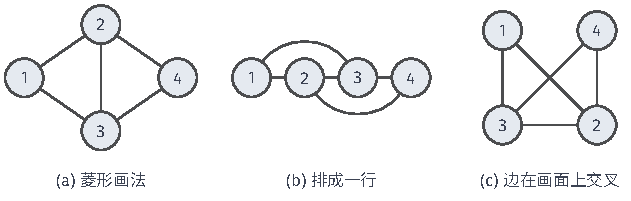
\includegraphics[width=106.765mm]{figures/01-basic-mathematics/04-graphs/tikz/c1-running-graph-drawings/figure.pdf}
  \caption{贯穿全章的四点五边图\eqref{eq:graph-conn-running-graph}的三种画法。顶点位置、线段形状和交叉情况都不同，但边集都是$\{1,2\},\{1,3\},\{2,3\},\{2,4\},\{3,4\}$。(c)中两条对角边在画面上交叉，交叉处不是顶点。}
  \label{fig:graph-conn-running-drawings}
\end{figure}

\paragraph{简单图的约定}
定义~\ref{def:graph-conn-graph}要求边的两个端点不同，并且边集是普通集合，因此排除了两种情形：一个顶点连到自身的\term{自环}（self-loop），以及同一对顶点之间的多条\term{平行边}（parallel edges）。满足这两条限制的图称为\term{简单图}（simple graph），本部分默认讨论有限简单图。若实际问题需要两条平行道路分别记录收费，就要给每条边一个独立身份，不能再把边等同于端点对；这时后面诸如“$n$个顶点最多有$\binom n2$条边”的计数也不再成立。用到这类扩展时会明确指出。

顶点集为空的图只有空边集，它在少数边界情形中出现，例如删除全部顶点后的余图。凡是结论需要至少一个顶点，我们都会写明“非空图”。

\subsection{无向图与有向图}
\label{sec:graph-conn-directions}

道路可以双向通行，“任务$i$完成后才能开始任务$j$”却有先后。无序对$\{i,j\}$不区分两个端点的次序，不能记录后一种信息，因此需要有序对。

\begin{definition}[有向图]
\label{def:graph-conn-digraph}
设$V$是有限集合，$E\subseteq\{(i,j)\in V\times V:i\neq j\}$，称$\mathcal G=(V,E)$为\term{有向图}（directed graph）。有序对$(i,j)\in E$称为从$i$到$j$的\term{弧}（arc），也记作$i\to j$；$i$是它的起点，$j$是它的终点。
\end{definition}

为了区分，以无序对为边的图也称\term{无向图}（undirected graph）。有向图的弧集仍记作$E$，弧数仍记作$m$；需要强调时再说“边或弧”。弧$i\to j$只允许从$i$一步到达$j$，并不包含反向的$j\to i$。

\paragraph{一条无向边不等于两条反向弧}
图~\ref{fig:graph-conn-direction-orientation}(a)(b)对照了无向边$\{u,v\}$与一对反向弧$(u,v),(v,u)$。两者都允许在$u,v$之间来回，但建模含义不同：无向边是一条连接，删除它就同时失去两个方向；两条弧则是两个独立对象，可以只删除其中一条，也可以分别附上不同的数值，例如上坡与下坡的不同用时。把无向图改写成有向图时，可以用一对反向弧代替每条边，但要记住这一步改变了“边”的个数和身份。

\paragraph{方向改变可达的范围}
图~\ref{fig:graph-conn-direction-orientation}(c)--(e)给同一条三点连接1—2—3赋予不同方向。无向时三个顶点两两可以互相到达；定向为$1\to2\to3$后，从$1$可以经$2$到达$3$，从$3$却哪里也去不了；定向为$1\to2\leftarrow3$后，$1$和$3$都只能到达$2$，彼此不能到达。可见方向不只是标注，它直接决定哪些顶点序列允许通行。

\begin{figure}[!htb]
  \centering
  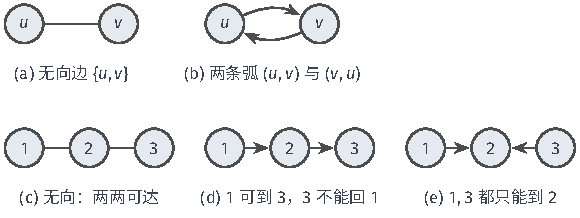
\includegraphics[width=98.189mm]{figures/01-basic-mathematics/04-graphs/tikz/c1-direction-orientation/figure.pdf}
  \caption{方向给连接附加的信息。上排：一条无向边与一对反向弧都允许在$u,v$之间往返，但后者的两条弧可以分别删除或另附数值。下排：同一条三点连接的无向形式(c)与两种定向(d)(e)，箭头决定了从哪个顶点能走到哪个顶点。}
  \label{fig:graph-conn-direction-orientation}
\end{figure}

\paragraph{底层无向图}
忽略有向图每条弧的方向，把$(i,j)$与$(j,i)$都换成无序对$\{i,j\}$（两者同时出现时只留一条边），得到的无向图称为原图的\term{底层无向图}（underlying undirected graph）。图~\ref{fig:graph-conn-direction-orientation}中(d)(e)的底层无向图都是(c)。这一步丢掉了依赖的先后：(c)中$3$能到达$1$，(d)中却不能，所以不能根据底层无向图的连接情况断言原有向图可以双向到达。第~\ref{sec:graph-connectivity-separation}节的弱连通正是建立在底层无向图上的概念，那里会再次比较两者。

\subsection{边权与属性}
\label{sec:graph-conn-weights}

图只说明哪些顶点直接相连。许多问题还需要每条连接上的一个数：道路有多长，管道每秒最多输送多少，两个样本有多相似。

\paragraph{边权的三种常见语义}
给每条边$\{i,j\}$（或弧$(i,j)$）附加一个实数，称为\term{边权}（edge weight）。图~\ref{fig:graph-conn-weight-semantics}在同一个边集上附加了同一组数，却给出三种读法。读作长度$\ell_{i,j}$时，数值沿路线逐条相加，路线$1,2,4$的总长是$2+1=3$，越小越好；读作容量$c_{i,j}$时，数值是通过这条边的流量上限，边$\{1,3\}$上至多通过$1$个单位，容量不沿路线相加；读作相似度$w_{i,j}$时，权重越大，后续计算越强地要求两端取值接近。同一个数字$1$在三种问题里参与的运算完全不同，所以拿到一张带权图时，要先问清权重的用途，再选择方法。

\begin{figure}[!htb]
  \centering
  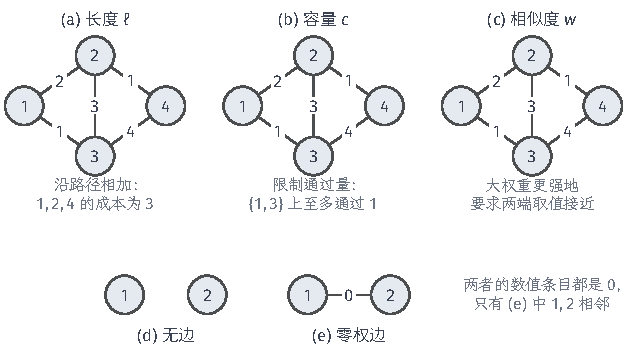
\includegraphics[width=106.768mm]{figures/01-basic-mathematics/04-graphs/tikz/c1-weight-semantics/figure.pdf}
  \caption{同一边集上的同一组边权在三种问题中的读法。(a)长度沿路线相加，路线$1,2,4$的总长为$3$；(b)容量限制单条边的通过量；(c)相似度越大，越要求两端取值接近。下排对照无边(d)与零权边(e)：二者在数值上都记为$0$，但只有(e)中顶点$1,2$相邻。}
  \label{fig:graph-conn-weight-semantics}
\end{figure}

\paragraph{无边与零权边}
边权为$0$并不等于没有边。零长度的道路表示免费通行，零容量的管道不能输送正流量，零相似度在加权求和中不贡献数值；但在这三种情形中，结构上的边都还在。图~\ref{fig:graph-conn-weight-semantics}(d)(e)中，两个顶点之间有没有边由边集决定，与边权是否为零无关：“能否一步到达”查边集，“沿边累计多少”查边权。第~\ref{sec:graph-representations}节用矩阵记录图时，这一区别会变成一个具体的存储问题。

边权能否为负，也由问题决定。负长度可以表示途经某处得到补贴，它会让最短路问题出现新的困难；谱方法则要求相似度非负。这些条件分别在第~\ref{chap:graph-optimization}章和第~\ref{chap:graph-spectral}章建立，本章不预设边权的符号。

\paragraph{顶点属性与边属性}
除了一个实数，边上还可以记录类别、时间等其他数据，顶点上也可以记录人口、坐标等数据，分别称为边属性和顶点属性。顶点的名称$1,2,3,4$只用来区分顶点，本身不是属性：第~\ref{sec:graph-isomorphism}节比较两张图时会看到，换一套名称不改变图的结构，而属性是否必须保持则要由问题声明。

\subsection{子图与诱导子图}
\label{sec:graph-conn-subgraphs}

研究道路网时，常常只关心其中一部分城市，或者想知道封闭几条道路后还剩什么。这两种操作都从原图取出一部分，但保留的东西不同。

\paragraph{子图}
若$V'\subseteq V$，$E'\subseteq E$，并且$E'$中每条边的两个端点都在$V'$中，称$\mathcal G'=(V',E')$是$\mathcal G$的\term{子图}（subgraph）。最后一条要求保证$\mathcal G'$本身仍是一张图，不会出现端点被删掉的边。两种基本操作都产生子图：删除一条边$e$只去掉这条边，顶点全部保留，记作$\mathcal G-e$；删除一个顶点集$S$则去掉$S$中的顶点以及所有至少有一个端点在$S$中的边，记作$\mathcal G-S$。

在图~\ref{fig:graph-conn-subgraph-induced}中，(b)(c)两个子图保留同一组顶点$\{1,2,3\}$，边集却不同：(b)保留三条边，(c)只保留$\{1,2\}$与$\{2,3\}$。所以只给出顶点集合，还不能确定一个一般子图；(d)则是只删除边$\{2,3\}$、保留全部顶点的子图。

\begin{figure}[!htb]
  \centering
  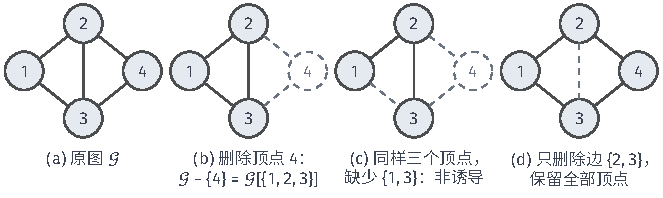
\includegraphics[width=112.000mm]{figures/01-basic-mathematics/04-graphs/tikz/c1-subgraph-induced/figure.pdf}
  \caption{贯穿图的几种子图，灰色虚线表示被删除的顶点或边。(b)删除顶点$4$及其两条边，恰好得到顶点集$\{1,2,3\}$上的诱导子图；(c)保留同样三个顶点，却漏掉了原图中的边$\{1,3\}$，是子图但不是诱导子图；(d)只删除一条边，顶点全部保留。}
  \label{fig:graph-conn-subgraph-induced}
\end{figure}

\paragraph{诱导子图}
只研究一部分顶点时，通常不希望悄悄改变这些顶点之间的关系。为此固定顶点子集，把原图中两端都在其中的边全部保留下来。

\begin{definition}[诱导子图]
\label{def:graph-conn-induced-subgraph}
设$S\subseteq V$。以$S$为顶点集、以$\{\{i,j\}\in E:i,j\in S\}$为边集的子图，称为$\mathcal G$在$S$上的\term{诱导子图}（induced subgraph），记作$\mathcal G[S]$。有向图的诱导子图保留两端都在$S$中的全部弧。
\end{definition}

诱导子图由顶点集唯一确定。图~\ref{fig:graph-conn-subgraph-induced}(b)是$\mathcal G[\{1,2,3\}]$，它必须保留三角形的三条边；(c)虽然顶点相同，但缺少$\{1,3\}$，不是诱导子图。删除顶点与取诱导子图互为补充：$\mathcal G-S=\mathcal G[V\setminus S]$。后面讨论删除一组顶点能否切断连接（第~\ref{sec:graph-connectivity-separation}节），以及第~\ref{chap:graph-traversal}章把图按分隔集分块时，用到的都是这一记号。

\section{邻接与路径}
\label{sec:graph-adjacency-paths}

贯穿图\eqref{eq:graph-conn-running-graph}中顶点$1$和$4$之间没有边，却可以先到$2$或$3$，再到$4$。“一步能到谁”由边集直接读出；“若干步能到谁”则要把边首尾相接。本节先描述一个顶点的直接邻居，再定义多步的行走和路径，区分无向环与有向环，最后建立可达关系。边上若有长度，怎样比较不同路线的总成本是第~\ref{sec:graph-shortest-paths}节的问题，这里只讨论哪些顶点序列允许通行。

\subsection{邻接、邻域与度}
\label{sec:graph-conn-neighborhoods}

在无向图中，若$\{i,j\}\in E$，称$i$与$j$\term{邻接}（adjacent），互为邻居。顶点$i$的全部邻居组成它的\term{邻域}（neighborhood）
\[
N(i)=\{j\in V:\{i,j\}\in E\},
\]
邻居的个数$d_i=|N(i)|$称为$i$的\term{度}（degree）。贯穿图中$N(1)=\{2,3\}$，$N(2)=\{1,3,4\}$，四个顶点的度依次为$2,3,3,2$。度只数直接邻居；$1$经过两步可以到达$4$，但$4$不计入$N(1)$。

\paragraph{有向图的两种邻域}
在有向图中，一条弧$i\to j$对两个端点的意义不同：对$i$来说$j$是下一步可以到达的顶点，对$j$来说$i$是能一步到达它的顶点。因此要分别定义出邻域与入邻域：
\[
N^+(i)=\{j:(i,j)\in E\},\qquad
N^-(i)=\{j:(j,i)\in E\}.
\]
二者的大小$d_i^+=|N^+(i)|$与$d_i^-=|N^-(i)|$分别称为\term{出度}（out-degree）与\term{入度}（in-degree）。以图~\ref{fig:graph-conn-direction-orientation}(e)的$1\to2\leftarrow3$为例，$N^-(2)=\{1,3\}$，$N^+(2)=\varnothing$：两个顶点能一步到达$2$，从$2$出发却一步也走不了。报告“$2$的邻居”时若不说明方向，就可能把入邻居误当成下一步可以到达的顶点。

\paragraph{度数和与边数}
把每个顶点的度加起来，会得到一个只与边数有关的量。考虑所有“顶点—边”配对$(i,e)$，其中$i$是边$e$的端点。按顶点分组，顶点$i$出现在$d_i$个配对中；按边分组，每条边恰有两个端点，出现在两个配对中。两种分组数的是同一批配对，所以
\begin{equation}
\sum_{i\in V}d_i=2m.
\label{eq:graph-conn-handshake}
\end{equation}
贯穿图中$2+3+3+2=10=2\times5$。由此还可知，度为奇数的顶点个数必是偶数，否则左边为奇数。在有向图中，每条弧恰好贡献一个出度和一个入度，同样的分组给出
\[
\sum_{i\in V}d_i^+=\sum_{i\in V}d_i^-=m;
\]
例如图~\ref{fig:graph-conn-direction-orientation}(d)的$1\to2\to3$中，出度为$1,1,0$，入度为$0,1,1$，两组之和都是弧数$2$。这里的度只数结构上的边，不涉及边权；把邻边权重累加起来的加权度在第~\ref{sec:graph-vertex-edge-functions}节另行定义。

\subsection{行走、路径与环}
\label{sec:graph-conn-walks-paths}

把相邻的边首尾相接，就得到一串顶点。是否允许重复经过同一个顶点，会得到用途不同的对象：反复传播、来回巡视的过程允许重复，一条实际路线通常不允许。

\begin{definition}[行走与路径]
\label{def:graph-conn-walk-path}
设$\mathcal G=(V,E)$是无向图。顶点序列$(v_0,\ldots,v_k)$若对每个$r=1,\ldots,k$都有$\{v_{r-1},v_r\}\in E$，就称为从$v_0$到$v_k$的一条\term{行走}（walk），$k$称为它的长度，即经过的边数。若行走中的顶点两两不同，就称为一条简单\term{路径}（path）。
\end{definition}

行走允许重复经过顶点和边；单个顶点$(v_0)$是长度为零的行走，也是长度为零的路径。本部分不加修饰的“路径”都指简单路径。图~\ref{fig:graph-conn-walk-path-cycle}(a)的$(1,2,3,1,2)$是长度为$4$的行走，它两次经过边$\{1,2\}$；(b)的$(1,2,4)$是长度为$2$的路径。

\begin{figure}[!htb]
  \centering
  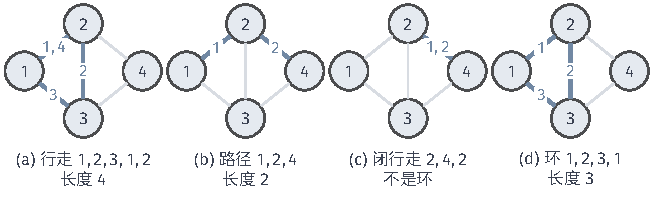
\includegraphics[width=110.688mm]{figures/01-basic-mathematics/04-graphs/tikz/c1-walk-path-cycle/figure.pdf}
  \caption{贯穿图上的四种顶点序列。蓝色粗线是经过的边，边旁数字是经过该边的步序，浅灰色是未经过的边。(a)行走可以重复经过边$\{1,2\}$；(b)路径不重复顶点；(c)沿一条边去而复返得到闭行走，但它不是环；(d)绕三角形一周的环除首尾外不重复顶点。}
  \label{fig:graph-conn-walk-path-cycle}
\end{figure}

\paragraph{闭行走与环}
首尾相同（$v_0=v_k$）的行走称为\term{闭行走}（closed walk）。闭合并不意味着绕成了一圈：图~\ref{fig:graph-conn-walk-path-cycle}(c)的$(2,4,2)$沿边$\{2,4\}$去而复返，是长度为$2$的闭行走，却没有围出任何区域。为了排除这种情形，把长度$k\geq3$、且$v_0,v_1,\ldots,v_{k-1}$两两不同的闭行走称为\term{环}（cycle）。长度下限来自简单图的约定：长度为$1$的闭行走需要自环，长度为$2$的闭行走$(v_0,v_1,v_0)$只能沿同一条边往返。图~\ref{fig:graph-conn-walk-path-cycle}(d)的$(1,2,3,1)$是长度为$3$的环。

同一个环可以从不同顶点出发、沿两个方向书写，例如$(1,2,3,1)$、$(2,3,1,2)$和$(1,3,2,1)$经过的是同一组边。计数环或比较两个环时，我们把经过同一组边的序列看成同一个环。

\subsection{有向路径与有向无环图}
\label{sec:graph-conn-dag}

任务依赖要求每一步都顺着箭头走：从任务$i$出发，只能走到依赖$i$的任务。把定义~\ref{def:graph-conn-walk-path}中的条件$\{v_{r-1},v_r\}\in E$换成$(v_{r-1},v_r)\in E$，就得到有向行走与\term{有向路径}（directed path）；长度、闭合与顶点不重复的含义不变。

\paragraph{有向环}
除首尾外顶点两两不同、长度至少为$1$的有向闭行走称为\term{有向环}（directed cycle）。由于排除了自环，有向环的长度至少为$2$；与无向情形不同，长度为$2$的有向环是允许的。图~\ref{fig:graph-conn-directed-cycle-dag}(a)中两条反向弧$i\to j$和$j\to i$是两个不同的对象，$(i,j,i)$依次经过它们，构成一个有向环；而无向图中的$(2,4,2)$两次经过的是同一条边。图~\ref{fig:graph-conn-directed-cycle-dag}(b)的$(1,2,3,1)$每一步都顺着箭头，是长度为$3$的有向环。

\begin{figure}[!htb]
  \centering
  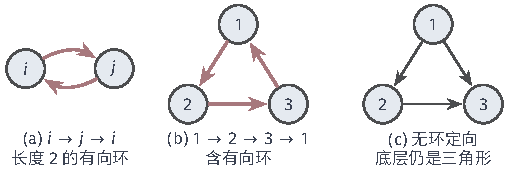
\includegraphics[width=85.937mm]{figures/01-basic-mathematics/04-graphs/tikz/c1-directed-cycle-dag/figure.pdf}
  \caption{有向环与有向无环图。红色弧组成有向环。(a)两条反向弧构成长度为$2$的有向环；(b)三角形的循环定向含有向环；(c)同一个三角形的另一种定向不含有向环，是有向无环图，尽管它的底层无向图是一个环。}
  \label{fig:graph-conn-directed-cycle-dag}
\end{figure}

\paragraph{有向无环图}
如果任务之间的依赖形成有向环，例如$1$等$2$、$2$等$3$、$3$又等$1$，这组任务就无法按任何次序全部完成。不含有向环的依赖才可能排出顺序。

\begin{definition}[有向无环图]
\label{def:graph-conn-dag}
不含有向环的有向图称为\term{有向无环图}（directed acyclic graph，DAG）。
\end{definition}

“无环”只针对有向环。图~\ref{fig:graph-conn-directed-cycle-dag}(c)的弧为$1\to2$、$1\to3$、$2\to3$，逐个检查长度为$2$和$3$的闭合序列，没有一个能每步都顺着箭头：例如$(1,2,3,1)$的最后一步需要弧$3\to1$，而图中只有$1\to3$。所以它是DAG，但去掉箭头后得到一个三角形，底层无向图是有环的。第~\ref{sec:graph-topological-order}节的拓扑排序要求的正是有向无环，不能换成“底层无向图无环”这个更强的条件。

\subsection{可达性}
\label{sec:graph-conn-reachability}

前面的定义描述的是具体的顶点序列。很多问题只关心“能不能到”，而不关心怎么到。

\paragraph{可达关系}
若存在从$i$到$j$的行走，称$j$从$i$\term{可达}（reachable）；有向图中要求有向行走。行走允许重复顶点，使用起来比路径方便：从$i$到$j$的行走接上从$j$到$k$的行走，仍是一条行走，而两条路径首尾相接后可能重复经过顶点。下面的引理说明，判断可达时用行走还是路径并没有区别。

\begin{lemma}[行走中含有路径]
\label{lem:graph-conn-walk-contains-path}
在无向图或有向图中，若存在从$i$到$j$的行走，则存在从$i$到$j$的路径，并且它的顶点和边都取自这条行走。
\end{lemma}

\begin{proof}
在从$i$到$j$、顶点和边都取自原行走的所有行走中，取长度最短的一条$(v_0,\ldots,v_k)$。若它不是路径，则有$s<t$使$v_s=v_t$。删去中间段$v_{s+1},\ldots,v_t$，得到$(v_0,\ldots,v_s,v_{t+1},\ldots,v_k)$：原来从$v_t$出发的那一步现在从$v_s=v_t$出发，因此每一步仍沿原有的边或弧，而长度减少了$t-s>0$，与长度最短矛盾。所以最短的那条行走就是路径。
\end{proof}

由定义和引理，可达关系有以下性质。零长度行走使每个顶点从自身可达，即自反性；行走首尾相接说明传递性；在无向图中把行走倒过来走仍是行走，所以还有对称性。因此无向图上的可达关系是第~\ref{sec:prelim-equivalence-relations}节意义下的等价关系，下一节将据此划分连通分量。

\paragraph{有向图中可达不对称}
有向图中倒过来走需要反向弧，对称性一般不成立。在图~\ref{fig:graph-conn-direction-orientation}(d)的单向链$1\to2\to3$中，$3$从$1$可达，$1$却不从$3$可达。为了描述这种单向的关系，把一步关系与多步关系分别命名：$N^-(j)$中的顶点称为$j$的直接\term{前驱}（predecessor），$N^+(j)$中的顶点称为直接\term{后继}（successor）；能经过一条或多条弧到达$j$的其他顶点称为$j$的\term{祖先}（ancestor），从$j$出发经过一条或多条弧能到达的其他顶点称为$j$的\term{后代}（descendant）。本部分约定祖先与后代都不含$j$自身。

在单向链中，$3$的直接前驱只有$2$，祖先则是$\{1,2\}$；$1$的后代是$\{2,3\}$，$3$没有后代。有向环上的两个不同顶点可以互为祖先，例如图~\ref{fig:graph-conn-directed-cycle-dag}(b)中的$1$和$2$；在DAG中这不可能发生。若$i\neq j$互为祖先，把$i$到$j$与$j$到$i$的两条有向路径拼起来，得到一条长度至少为$2$的有向闭行走$(v_0,\ldots,v_k)$，其中$v_0=v_k$。在所有满足$s<t$、$v_s=v_t$的位置对中取$t-s$最小的一对，则$(v_s,\ldots,v_t)$除首尾外不重复顶点；它的长度不能为$1$（没有自环），所以是一个有向环，与DAG的定义矛盾。可达的不对称性使有向图的“连通”需要两种不同的定义，这是下一节的内容。

\section{连通与分隔}
\label{sec:graph-connectivity-separation}

上一节的可达关系一次只回答两个顶点之间的问题。道路网规划还需要整体的回答：全部城市分成几片互相到达的区域，封闭哪些路口或道路会把区域切开。本节先用可达关系把顶点集划分为连通分量，再对有向图区分强、弱两种连通，最后研究删除顶点或边怎样改变连接。这里只讨论结构上的路径是否存在，不涉及概率中的条件独立；后者有自己的分离判据，留到后续关于推断的部分。

\subsection{无向图的连通分量}
\label{sec:graph-conn-components}

在无向图中，可达关系是等价关系（第~\ref{sec:graph-conn-reachability}小节）。由定理~\ref{thm:sets-equivalence-partition}，它的等价类构成顶点集的一个划分。

\begin{definition}[连通分量]
\label{def:graph-conn-component}
无向图$\mathcal G=(V,E)$中可达关系的每个等价类$C\subseteq V$称为$\mathcal G$的一个\term{连通分量}（connected component）；有时也把诱导子图$\mathcal G[C]$称为连通分量。若$\mathcal G$非空且恰有一个连通分量，即任意两个顶点之间都有路径，就称$\mathcal G$是\term{连通}（connected）的。
\end{definition}

这个划分有三条直接的性质。第一，同一分量中任意两点可达，而且连接它们的路径不会离开该分量，因为路径上的每个顶点都与起点可达；所以$\mathcal G[C]$本身是连通图。第二，不同分量之间没有边：若$i\in C$、$j\in C'$之间有边，则$j$从$i$可达，二者应属同一分量。第三，划分由图唯一确定，因为等价类只取决于可达关系本身，与我们从哪个顶点开始寻找无关。

图~\ref{fig:graph-conn-components}(a)是三角形$\{1,2,3\}$加上孤立顶点$4$。$4$没有邻居，只与自身可达，单独构成一个分量，所以这张图有两个分量$\{1,2,3\}$与$\{4\}$，不连通。对顶点集为空的图，可达关系没有等价类，分量数为$0$；按定义它不算连通图。凡是用“恰有一个分量”判断连通性的论证，都需要先排除这个边界情形。

\begin{figure}[!htb]
  \centering
  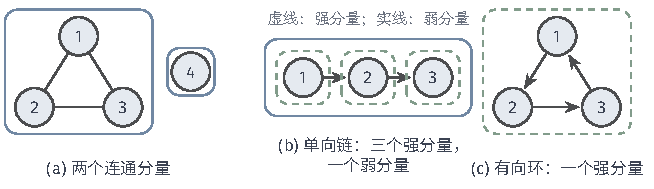
\includegraphics[width=110.808mm]{figures/01-basic-mathematics/04-graphs/tikz/c1-components/figure.pdf}
  \caption{连通分量。蓝色实线框是无向图或底层无向图的连通分量，绿色虚线框是强连通分量。(a)孤立点自成一个分量；(b)单向链$1\to2\to3$忽略方向后连成一片，但没有两个顶点能互相到达，每个顶点自成一个强分量；(c)有向环上任意两个顶点都能互相到达，三个顶点属于同一个强分量。}
  \label{fig:graph-conn-components}
\end{figure}

\paragraph{删除边与替代路径}
连通性取决于是否还有替代路径，而不只取决于边的数目。在贯穿图中删除边$\{2,3\}$，$2$与$3$仍可经$1$或$4$相连，图依然连通；在图~\ref{fig:graph-conn-cut-bridge}(a)中删除连接两个三角形的边$\{3,4\}$，两侧之间就再没有路径，图分成两个分量。两次都只删除了一条边，结果不同的原因是前者的边位于环上，环的另一侧提供了替代路径。第~\ref{sec:graph-conn-separators}小节会把这一观察写成桥的判别条件。

\subsection{强连通与弱连通}
\label{sec:graph-conn-strong-weak}

有向图中可达不对称，“$j$从$i$可达”不能像无向图那样直接用来划分顶点。有两种自然的修补：要求双向都可达，或者干脆忽略方向。

\paragraph{强连通分量}
若$j$从$i$可达且$i$从$j$可达，称$i,j$相互可达。相互可达关系是自反的（零长度行走）、对称的（定义本身对$i,j$对称）、传递的（两个方向分别把行走首尾相接），因此是等价关系。它的等价类称为\term{强连通分量}（strongly connected component）；若有向图非空且只有一个强连通分量，即任意有序顶点对$(i,j)$之间都有从$i$到$j$的有向路径，就称它\term{强连通}（strongly connected）。

图~\ref{fig:graph-conn-components}(b)的单向链中，$1$能到$3$而$3$不能到$1$，任何两个不同顶点都不相互可达，所以三个顶点各自构成一个强分量。(c)的有向环中，从任一顶点出发沿环走一段就能到达其他任一顶点，三个顶点同属一个强分量，图是强连通的。可见强分量把“绕得回来”的顶点归在一起；把单向可达的顶点合进同一个强分量是错误的。

\paragraph{弱连通分量}
忽略方向后，用底层无向图（第~\ref{sec:graph-conn-directions}小节）的连通分量来划分顶点，所得的分量称为原图的\term{弱连通分量}（weakly connected component）；底层无向图连通时，称原有向图\term{弱连通}（weakly connected）。图~\ref{fig:graph-conn-components}(b)的单向链去掉箭头后是一条路径，只有一个弱分量。

两种分量的关系是单向的。每条有向路径去掉箭头后都是底层无向图中的路径，所以相互可达的两个顶点必在同一个弱分量中：每个强分量都包含在某个弱分量之内，强连通蕴含弱连通。反过来不成立，单向链弱连通但不强连通，其中$3$到不了$1$。所以弱连通只说明忽略方向后连成一片，不保证任何两个顶点能双向到达。怎样在线性时间内求出全部强分量，是第~\ref{sec:graph-connectivity-computation}节的内容。

\subsection{分隔集、割点与桥}
\label{sec:graph-conn-separators}

连通分量描述的是现状；规划者还关心脆弱性：封闭哪些路口能把两个区域隔开，哪个单独的路口或哪条单独的道路一旦失效就会让网络断开。

\paragraph{分隔集}
要把两组顶点隔开，就要删除一些别的顶点，使两组之间不再有路径。被删除的顶点不能属于要隔开的两组本身。

\begin{definition}[分隔]
\label{def:graph-conn-separation}
设$A,B,S\subseteq V$两两不相交。若在$\mathcal G-S$中不存在从$A$中顶点到$B$中顶点的路径，就称$S$\term{分隔}（separate）$A$与$B$，称$S$为$A$与$B$之间的一个\term{分隔集}（separator）。
\end{definition}

等价地，$\mathcal G$中从$A$到$B$的每条路径都至少经过$S$中的一个顶点：若某条路径避开了$S$，它在$\mathcal G-S$中仍然存在。这个等价说法提醒我们，验证一个候选集要检查全部路径，找到一条被阻断的路径并不够。

在图~\ref{fig:graph-conn-separator-sets}中取$A=\{1\}$、$B=\{4\}$。候选集$S=\{2\}$阻断了路径$(1,2,4)$，但$\mathcal G-\{2\}$中仍有路径$(1,3,4)$，所以$\{2\}$不分隔$1$与$4$；删除$S=\{2,3\}$后，$1$的邻居全部被删除，$1$与$4$之间不再有路径，$\{2,3\}$才是分隔集。若$A$与$B$在原图中已经位于不同分量，空集就分隔它们，因为不删除任何顶点时本来就没有路径。

\begin{figure}[!htb]
  \centering
  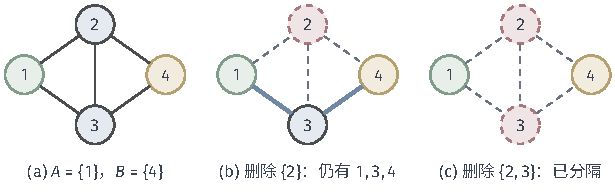
\includegraphics[width=104.186mm]{figures/01-basic-mathematics/04-graphs/tikz/c1-separator-sets/figure.pdf}
  \caption{在贯穿图中检验分隔集，$A=\{1\}$为绿色，$B=\{4\}$为黄色，被删除的候选集$S$为红色虚线顶点。(b)删除$\{2\}$后蓝色路径$(1,3,4)$仍然存在，$\{2\}$不是分隔集；(c)删除$\{2,3\}$后从$1$到$4$没有路径，$\{2,3\}$分隔$\{1\}$与$\{4\}$。}
  \label{fig:graph-conn-separator-sets}
\end{figure}

不指定$A,B$时，也可以只问删除一组顶点后图是否断开。对连通图$\mathcal G$，若$\mathcal G-S$不连通，则$S$分隔$\mathcal G-S$中任意两个不同分量的顶点集。例如贯穿图删除$\{2,3\}$后余下$\{1\}$与$\{4\}$两个分量。第~\ref{sec:graph-separator-blocks}节将沿这样的分隔集把图分成可以分别处理的块。

\paragraph{割点与桥}
最脆弱的情形是只删除一个顶点或一条边就增加了分量数。删除顶点$v$后$\mathcal G-\{v\}$的分量数大于$\mathcal G$的分量数，称$v$为\term{割点}（cut vertex）；删除边$e$后$\mathcal G-e$的分量数大于$\mathcal G$的分量数，称$e$为\term{桥}（bridge）。

图~\ref{fig:graph-conn-cut-bridge}(a)由两个三角形和连接它们的边$\{3,4\}$组成。删除$3$后，$\{1,2\}$与$\{4,5,6\}$分开，$4$同理，所以$3,4$是割点；删除边$\{3,4\}$也把两侧分开，它是桥。三角形内部的边都不是桥，三角形顶点$1,2,5,6$也不是割点。(b)的链中，中间顶点$2$是割点，两条边都是桥；(c)的三角形中，删除任意一个顶点或一条边，剩下的部分仍然连通。

\begin{figure}[!htb]
  \centering
  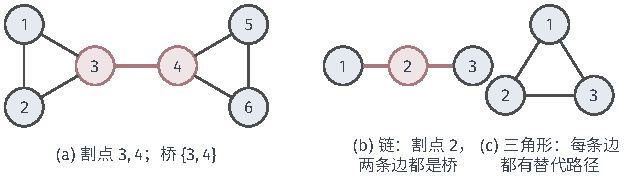
\includegraphics[width=106.765mm]{figures/01-basic-mathematics/04-graphs/tikz/c1-cut-vertex-bridge/figure.pdf}
  \caption{割点与桥，红色顶点为割点，红色粗边为桥。(a)两个三角形由一条边相连，这条边是桥，它的两个端点是割点；(b)链上每条边都是桥，中间顶点是割点，端点$1,3$虽是桥的端点却不是割点；(c)三角形的每条边都位于环上，删除任何一条边或一个顶点都不会断开。}
  \label{fig:graph-conn-cut-bridge}
\end{figure}

\paragraph{为什么边位于环上就不是桥}
设$e=\{i,j\}$。删除$e$只可能拆开$e$所在的那个分量$C$：$C$中任一顶点$x$在原图中有到$i$的路径，若这条路径不经过$e$，删除后它仍连到$i$；若经过$e$，取它第一次到达$i$或$j$之前的部分，删除后$x$仍连到$i$或$j$。所以$\mathcal G-e$中$C$至多分成$i$所在和$j$所在两部分，分量数至多增加$1$。由此得到判别条件：$e$是桥，当且仅当$\mathcal G-e$中没有从$i$到$j$的路径。

若$e$位于某个环上，沿环的另一侧就是$\mathcal G-e$中从$i$到$j$的路径，$e$不是桥。反过来，若$\mathcal G-e$中有从$i$到$j$的路径$P$，它不经过$e$，长度至少为$2$，接上$e$就得到一个环。所以一条边是桥，当且仅当它不在任何环上。这正是图~\ref{fig:graph-conn-cut-bridge}中三角形与链的区别。

\paragraph{顶点分隔与边分隔不同}
删除一个顶点会同时删除它的全部邻边，可能把分量拆成很多块：在一个中心顶点与其余每个顶点各连一条边的星形图中，删除中心顶点后，其余每个顶点都自成一个分量。删除一条边却如上所述至多增加一个分量。此外，桥的端点不一定是割点，例如图~\ref{fig:graph-conn-cut-bridge}(b)的端点$1$；没有桥的图也可能有割点，例如两个三角形共用一个顶点时，共用的顶点是割点，而每条边都在某个三角形上。所以“删点能否断开”与“删边能否断开”需要分别检查。

\section{树与森林}
\label{sec:graph-trees-forests}

上一节看到，边位于环上时删掉它不会断开连接，环提供的是冗余的替代路径。反过来，若要用尽量少的道路把一组城市连起来，就不应保留任何环。本节研究连通而无环的结构：先给出树和森林的定义，再证明树中路径唯一、$n$个顶点的树恰有$n-1$条边，然后在树上选根来组织父子关系，最后从一般连通图中抽取覆盖全部顶点的树。这些结论是第~\ref{chap:graph-traversal}章遍历结果、第~\ref{sec:graph-minimum-spanning-tree}节最小生成树和第~\ref{sec:graph-tree-dp}节树上动态规划的共同基础。

\subsection{树与森林的定义}
\label{sec:graph-conn-tree-definition}

连通保证任意两点之间有路线，无环保证没有多余的路线。同时要求这两点，就得到树。

\begin{definition}[树与森林]
\label{def:graph-conn-tree}
非空、连通且不含环的无向图称为\term{树}（tree）。不含环的无向图称为\term{森林}（forest）。
\end{definition}

森林的每个连通分量都是连通且无环的，因而都是一棵树，“森林”的名称由此而来。不同分量之间没有边，所以森林整体未必连通，只有恰好一个分量的森林才是树。图~\ref{fig:graph-conn-tree-forest}给出几个对照：(a)的链和(b)的星形都是树，树可以有分支，不必排成一条线；(c)的三角形连通但有环，不是树；(d)有三个分量$\{1,2\}$、$\{3,4,5\}$和$\{6\}$，每个都是树，整体是森林而不是树。

\begin{figure}[!htb]
  \centering
  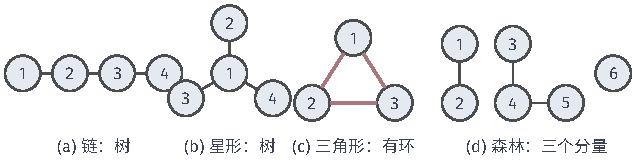
\includegraphics[width=107.685mm]{figures/01-basic-mathematics/04-graphs/tikz/c1-tree-forest/figure.pdf}
  \caption{树、森林与非树的对照。(a)链与(b)星形都是树，后者有分支；(c)三角形连通但含有红色标出的环，不是树；(d)由三个互不相连的树组成的森林，其中孤立顶点$6$是一棵单点树。}
  \label{fig:graph-conn-tree-forest}
\end{figure}

两个边界情形需要单独说明。只有一个顶点、没有边的图是树，称为单点树；图~\ref{fig:graph-conn-tree-forest}(d)中的顶点$6$就是森林里的一棵单点树，所以树中的顶点不必都有邻边。顶点集为空的图不含环，按定义是森林，称为空森林，它有$0$个分量；但树要求非空，所以空图不是树。

\subsection{树的基本性质}
\label{sec:graph-conn-tree-properties}

树的定义由连通和无环两条组成，这两条恰好对应路径的存在与唯一。下面先证明这一点，再用叶顶点数出树的边数。

\paragraph{路径唯一性}
若两点之间有两条不同的路径，它们分开以后终究要在某处会合，分开与会合之间的两段就围成一个环。反过来，环上相邻的两点既有一条边直接相连，又可以沿环的另一侧到达。这两个观察合起来给出下面的等价刻画。

\begin{theorem}[树中路径唯一]
\label{thm:graph-conn-tree-unique-path}
设$\mathcal G$是非空无向图。$\mathcal G$是树，当且仅当任意两个顶点之间恰有一条路径。
\end{theorem}

\begin{proof}
先设$\mathcal G$是树。连通性保证任意两点$u,v$之间至少有一条路径。假设有两条不同的路径$P=(p_0,\ldots,p_a)$与$Q=(q_0,\ldots,q_b)$，$p_0=q_0=u$，$p_a=q_b=v$。一条不能是另一条的真前段，否则较长的那条会两次经过$v$；所以存在最小的$s$使$p_{s+1}\neq q_{s+1}$，记$x=p_s=q_s$，两条路径在$x$处分开。由于$v$同时在两条路径上，可以取$P$在$x$之后第一个也出现在$Q$中$x$之后的顶点$y$。

$P$从$x$到$y$的一段与$Q$从$x$到$y$的一段除端点外没有公共顶点：$P$这一段的中间顶点按$y$的取法不在$Q$中$x$之后的部分，又因为$P$是路径，也不在$P$与$Q$共有的$x$之前的部分。沿$P$从$x$走到$y$，再沿$Q$倒着从$y$走回$x$，就得到一个除首尾外不重复顶点的闭行走。两段不能都只有一条边，否则$p_{s+1}=y=q_{s+1}$；所以它的长度至少为$3$，是一个环，与树无环矛盾。图~\ref{fig:graph-conn-tree-properties}(a)画出了这个构造。

反过来，设任意两点之间恰有一条路径。路径的存在说明$\mathcal G$连通。若$\mathcal G$含环$(c_0,c_1,\ldots,c_{k-1},c_0)$，$k\geq3$，则$(c_0,c_1)$与$(c_0,c_{k-1},c_{k-2},\ldots,c_1)$是从$c_0$到$c_1$的两条不同路径，与唯一性矛盾。所以$\mathcal G$无环，是树。
\end{proof}

由这个定理，删除树的任意一条边$e=\{u,v\}$都会把树断开：$u,v$之间唯一的路径就是$(u,v)$本身，删除$e$后它们之间不再有路径。按第~\ref{sec:graph-conn-separators}小节的论证，树恰好分成$u$所在与$v$所在的两部分，每部分仍连通且无环，是两棵较小的树。换言之，树的每条边都是桥，删去一条边就把树分成两侧。

\begin{figure}[!htb]
  \centering
  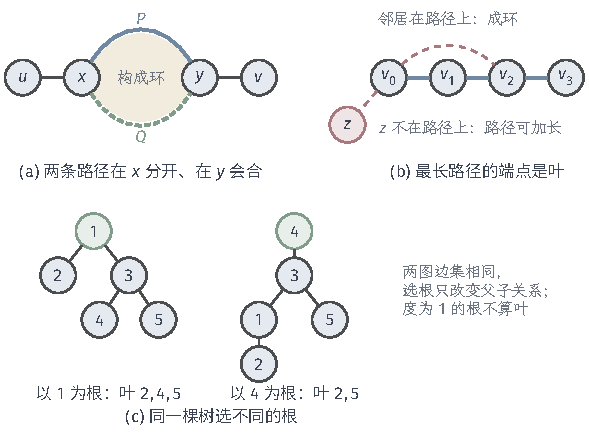
\includegraphics[width=99.688mm]{figures/01-basic-mathematics/04-graphs/tikz/c1-tree-properties/figure.pdf}
  \caption{树的性质的证明示意与选根。(a)两条不同的路径$P$（蓝色实线）与$Q$（绿色虚线）在$x$分开、在$y$第一次会合，二者之间的部分（黄色区域的边界）构成一个环。(b)若最长路径的端点$v_0$还有别的邻居，这个邻居不在路径上时可以把路径加长，在路径上时则形成环，两种情形都不可能。(c)同一棵树分别以$1$和$4$为根（绿色），边集不变，父子关系和叶的集合随根改变。}
  \label{fig:graph-conn-tree-properties}
\end{figure}

\paragraph{叶的存在}
数树的边数要用到度为$1$的顶点。无向图中度为$1$的顶点称为\term{叶}（leaf）。

\begin{lemma}[树有叶]
\label{lem:graph-conn-tree-leaves}
至少有两个顶点的树至少有两个叶。
\end{lemma}

\begin{proof}
树有限，路径只有有限条，取一条最长的路径$P=(v_0,\ldots,v_k)$。树连通且至少有两个顶点，所以有边，$k\geq1$。$v_1$是$v_0$的邻居。若$v_0$另有邻居$z\neq v_1$，分两种情形。若$z$不在$P$上，$(z,v_0,v_1,\ldots,v_k)$是一条更长的路径，与$P$最长矛盾；若$z=v_t$在$P$上，则$t\geq2$，$(v_0,v_1,\ldots,v_t,v_0)$是长度为$t+1\geq3$的环，与树无环矛盾。所以$d_{v_0}=1$。同理$d_{v_k}=1$，而$v_0\neq v_k$，树至少有两个叶。
\end{proof}

\paragraph{边数}
叶只与一个顶点相连，删掉它不会断开其余部分。这使我们能对顶点数归纳。

\begin{theorem}[树的边数]
\label{thm:graph-conn-tree-edges}
有$n$个顶点的树恰有$n-1$条边。
\end{theorem}

\begin{proof}
对$n$归纳。$n=1$时单点树没有边。设$n\geq2$，并设结论对$n-1$个顶点的树成立。由引理~\ref{lem:graph-conn-tree-leaves}，树$\mathcal T$有一个叶$v$，它只有一条邻边。考虑$\mathcal T-\{v\}$：它无环，因为删除顶点不会产生新环；它连通，因为$\mathcal T$中连接另外两个顶点的路径不会经过$v$——路径的中间顶点要有两条路径上的邻边，而$v$的度为$1$。所以$\mathcal T-\{v\}$是有$n-1$个顶点的树，由归纳假设有$n-2$条边。删除$v$只去掉一条边，$\mathcal T$有$n-1$条边。
\end{proof}

\paragraph{用边数判断树}
定理~\ref{thm:graph-conn-tree-edges}的逆命题需要加上连通的条件。先说明任何连通图都能用$n-1$条边连成一棵树，再比较边数。

设$\mathcal G$连通，任取一个顶点$r$，令已选顶点集$S=\{r\}$、已选边集$F=\varnothing$。只要$S\neq V$，就取一个$S$外的顶点$t$和一条从$r$到$t$的路径；路径从$S$内出发、在$S$外结束，其中必有一步从$S$内的顶点走到$S$外的顶点，把这一步的边加入$F$，把它的$S$外端点加入$S$。每一步恰好增加一个顶点和一条边，所以$n-1$步后$S=V$，$|F|=n-1$。

所得的$(V,F)$连通，因为每个新顶点都通过一条边连到先前已选的顶点上，归纳可知每个顶点都连到$r$。它也无环：若$F$中有环，取环上最后加入$S$的顶点$t$，它在环上的两个邻居都比它先加入。$F$中的每条边都在它的较晚端点加入时选出，并且连到一个更早的顶点；所以$t$与更早顶点之间的边只有$t$加入时选出的那一条，不可能同时连到环上两个更早的邻居，矛盾。因此$(V,F)$是一棵树。

\begin{theorem}[连通且$n-1$条边的图是树]
\label{thm:graph-conn-connected-tree-test}
设$\mathcal G$是有$n\geq1$个顶点的连通无向图。若$\mathcal G$恰有$n-1$条边，则$\mathcal G$是树。
\end{theorem}

\begin{proof}
按上面的构造从$\mathcal G$中选出$n-1$条边组成树$(V,F)$。$F\subseteq E$且$|F|=n-1=|E|$，所以$F=E$，$\mathcal G=(V,F)$本身就是树。
\end{proof}

连通的条件不能去掉。三角形加一个孤立顶点（图~\ref{fig:graph-conn-components}(a)）有$4$个顶点、$3$条边，恰好满足“$n-1$条边”，却既不连通又有环，不是树。只数边可能少看了连接，也可能把边浪费在环上。

\subsection{有根树}
\label{sec:graph-conn-rooted-trees}

在家谱、文件目录或分治计算中，树上的顶点有上下层次。路径唯一性使我们可以从任意一个顶点出发，把整棵树组织成这样的层次。

\paragraph{父节点、子节点与子树}
在树$\mathcal T$中选定一个顶点$r$作为根，得到\term{有根树}（rooted tree）。对每个$v\neq r$，从$r$到$v$有唯一的路径，路径上紧挨在$v$之前的顶点称为$v$的\term{父节点}（parent），$v$称为它的\term{子节点}（child）。根没有父节点，其余每个顶点恰有一个父节点。从$r$到$u$的路径经过$v$的那些顶点$u$（包括$v$本身）组成以$v$为根的\term{子树}（subtree）。在有根树中，没有子节点的顶点称为叶。

图~\ref{fig:graph-conn-tree-properties}(c)是同一棵树以两种方式选根。以$1$为根时，$3$的父节点是$1$，子节点是$4,5$，叶是$2,4,5$；以$4$为根时，$3$的父节点变成$4$，子节点变成$1,5$，叶是$2,5$。注意根$4$的度为$1$，在无向树中是叶，在以它为根的有根树中却有子节点、不算叶；两种“叶”的含义只在根上可能不同。

\paragraph{选根只附加组织方式}
两种选根下边集完全相同，选根没有增删任何边，只是规定了每条边上哪一端是父节点。父子关系由选根唯一确定，换一个根就会改变。若愿意，也可以把每条边定向为从父节点指向子节点，得到一张有向图，其中每个顶点的直接前驱就是父节点；但有根树的方向来自选根，而一般有向图的弧方向是原始数据的一部分，两者不应混同。第~\ref{sec:graph-tree-dp}节在有根树上自下而上计算时，正是利用“每个子树只通过它的根与外界相连”这一点。

\subsection{生成树与生成森林}
\label{sec:graph-conn-spanning-trees}

道路网中常要选出一部分道路，使所有城市仍然连通且没有多余的环，例如只维护最少的道路，或在网络中规定一套不会循环转发的线路。这就是在原图中保留全部顶点、只选部分边构成一棵树。

\begin{definition}[生成树与生成森林]
\label{def:graph-conn-spanning-tree}
设$\mathcal G=(V,E)$是无向图。若子图$(V,F)$，$F\subseteq E$，是一棵树，就称它为$\mathcal G$的\term{生成树}（spanning tree）。若$(V,F)$是森林，并且它的连通分量与$\mathcal G$的连通分量相同，就称它为$\mathcal G$的\term{生成森林}（spanning forest）。
\end{definition}

连通图一定有生成树，第~\ref{sec:graph-conn-tree-properties}小节逐个接入顶点的构造选出的$(V,F)$就是一棵。生成树要覆盖全部顶点，所以只有连通图才有生成树。对一般无向图，在每个连通分量上各取一棵生成树，合起来就是生成森林。

\paragraph{生成森林的边数}
设$\mathcal G$有$n$个顶点、$c$个连通分量，第$k$个分量有$n_k$个顶点，$n_1+\cdots+n_c=n$。由定理~\ref{thm:graph-conn-tree-edges}，第$k$个分量上的生成树有$n_k-1$条边，所以任何生成森林的边数都是
\begin{equation}
\sum_{k=1}^{c}(n_k-1)=n-c.
\label{eq:graph-conn-spanning-forest-edges}
\end{equation}
例如三角形加孤立顶点有$n=4$、$c=2$，生成森林有$2$条边：三角形中任选两条边，孤立顶点自成单点树。同一个计数也适用于任何森林：$n$个顶点、$c$个分量的森林恰有$n-c$条边。因此无环且有$n-1$条边的图只有一个分量，也是树。

\paragraph{生成树不唯一}
贯穿图\eqref{eq:graph-conn-running-graph}有$n=4$，它的每棵生成树都有$3$条边。从$5$条边中选$3$条共有$\binom53=10$种选法。若选出的$3$条边有环，环的长度只能是$3$，即恰好选中三角形$\{1,2,3\}$或$\{2,3,4\}$的三条边，这样的选法有$2$种。其余$8$种选法无环且有$n-1=3$条边，由上一段都是树。图~\ref{fig:graph-conn-spanning-trees}列出了这$8$棵生成树。

\begin{figure}[!htb]
  \centering
  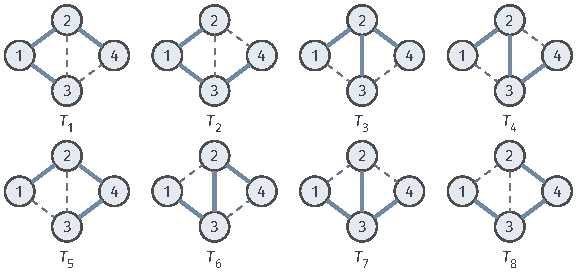
\includegraphics[width=97.652mm]{figures/01-basic-mathematics/04-graphs/tikz/c1-spanning-trees/figure.pdf}
  \caption{贯穿图的全部$8$棵生成树。蓝色粗线是树边，灰色虚线是被舍弃的原边。每棵生成树都有$3$条边并覆盖全部$4$个顶点；从$5$条边中选$3$条的$10$种选法里，只有恰好组成三角形$\{1,2,3\}$或$\{2,3,4\}$的两种不是树。}
  \label{fig:graph-conn-spanning-trees}
\end{figure}

\paragraph{抽取生成树会丢掉什么}
生成树保留了“全部顶点互相连通”，却舍弃了环所提供的替代路径，因此其他结构可能改变。以$T_2$（边$\{1,2\},\{1,3\},\{3,4\}$）为例：原图中$2,4$相邻，在$T_2$中却要经过$(2,1,3,4)$，路径长度从$1$变成$3$；原图删除任一顶点后仍连通，没有割点，而$T_2$中$1$和$3$都成了割点。所以在生成树上计算距离或分析脆弱性，结果一般不等于原图上的结果。

怎样用遍历高效地求出一棵生成树或生成森林，是第~\ref{chap:graph-traversal}章的内容；遍历得到的生成树只保证连通，不比较边权。当边带有建设成本时，从众多生成树中选出总成本最小的一棵，是第~\ref{sec:graph-minimum-spanning-tree}节研究的另一个问题。

\section{图的表示}
\label{sec:graph-representations}

前几节把图当作集合对$(V,E)$来推理。要让计算机处理一张图，还得决定怎样存储它。不同的算法反复执行的操作不同：有的逐条扫描所有边，有的反复列出一个顶点的全部邻居，有的要查询两个顶点之间是否有边，还有的要做矩阵运算。本节比较四种常用的表示，说明各自支持哪种访问、存储和访问代价怎样随顶点数$n$与边数$m$增长。代价用第~\ref{sec:comb-growth-scales}小节的记号$O(\cdot)$表示，例如“存储量为$O(n+m)$”指存储量不超过$n+m$的某个常数倍。图~\ref{fig:graph-conn-four-representations}把贯穿图的四种表示放在一起，供各小节对照。从矩阵出发构造图上的算子并研究其谱，集中在第~\ref{chap:graph-spectral}章。

\begin{figure}[!htb]
  \centering
  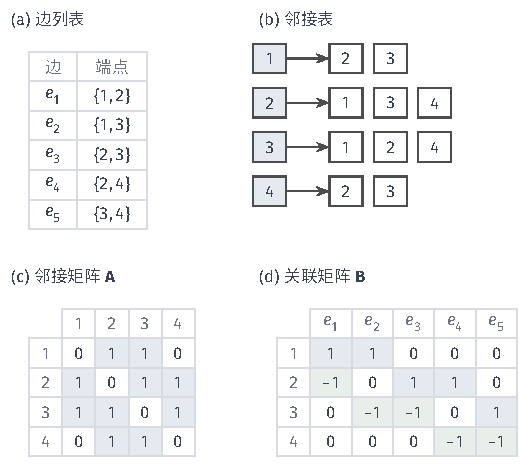
\includegraphics[width=89.524mm]{figures/01-basic-mathematics/04-graphs/tikz/c1-four-representations/figure.pdf}
  \caption{贯穿图的四种表示。(a)边列表逐条记录边的编号和端点；(b)邻接表为每个顶点（蓝色方框）列出邻居，每条无向边在两端各出现一次；(c)邻接矩阵按顶点次序记录每对顶点是否相邻，蓝色为$1$；(d)关联矩阵的每列对应一条边，按“小编号指向大编号”的记录方向，起点处为$1$（蓝色）、终点处为$-1$（绿色）。}
  \label{fig:graph-conn-four-representations}
\end{figure}

\subsection{边列表}
\label{sec:graph-conn-edge-list}

最直接的做法是把边一条条记下来。\term{边表}（edge list），也称边列表，为每条边保存一条记录：边的编号、两个端点，以及长度、容量等所需的属性。有向图的记录必须保存端点的次序，$(i,j)$与$(j,i)$是不同的弧。

图~\ref{fig:graph-conn-four-representations}(a)是贯穿图的边列表，$5$条无向边各占一条记录，记录中端点的先后没有意义。若扩展到有平行边的图，两条连接同一对顶点的边端点相同，只能靠编号区分，这时编号是记录中不可省略的部分。

\paragraph{访问方式与代价}
边列表除记录顶点集外只需$O(m)$的存储，适合需要逐条处理全部边的算法：例如按边权把所有边排序，或者在每一轮中把每条边都检查一遍。它的弱点是查询局部信息。要列出顶点$2$的邻居，或判断$\{1,4\}$是否为边，在没有额外索引时只能从头到尾扫描全部$m$条记录。第~\ref{sec:graph-minimum-spanning-tree}节按边权排序选边、第~\ref{sec:graph-shortest-paths}节逐轮检查每条边，用的都是这种访问方式。

\subsection{邻接表}
\label{sec:graph-conn-adjacency-list}

遍历一张图时，最频繁的操作是“列出当前顶点的全部邻居”。\term{邻接表}（adjacency list）为此而设计：给每个顶点保存一个列表，列出它的邻居，需要时连同对应边的属性一起保存。无向边$\{i,j\}$既出现在$i$的列表中，也出现在$j$的列表中；有向图的邻接表默认只保存出邻居，即$i$的列表是$N^+(i)$。

\paragraph{从边列表转换}
给$n$个顶点各建一个空列表，然后扫描边列表：遇到无向边$\{i,j\}$，就把$j$加入$i$的列表、把$i$加入$j$的列表；遇到弧$(i,j)$，只把$j$加入$i$的列表。转换用$O(n+m)$的时间。对贯穿图执行这一过程就得到图~\ref{fig:graph-conn-four-representations}(b)，顶点$2$的列表是$1,3,4$，长度恰好是度$d_2=3$。若算法还要沿弧反向查找，例如列出能一步到达$j$的全部顶点，就需要另建一份入邻居表，存储随之增加$O(m)$。

\paragraph{存储与访问代价}
邻接表有$n$个列表头；无向图的列表项共$\sum_i d_i=2m$个（式\eqref{eq:graph-conn-handshake}），有向图的出邻居表共$m$个。所以存储量为$O(n+m)$。列出顶点$i$的全部邻居只需读它自己的列表，时间与$d_i$成正比，不必触及与$i$无关的边；判断$\{i,j\}$是否为边则要在$i$的列表中查找，最坏需要$O(d_i)$时间。若一个算法对每个顶点都恰好列出一次邻居，总工作量就是$\sum_i(1+d_i)=n+2m$，即$O(n+m)$。第~\ref{chap:graph-traversal}章分析遍历的开销时，正是这样把实际访问次数累加起来。

\subsection{邻接矩阵}
\label{sec:graph-conn-adjacency-matrix}

查询“$i,j$是否相邻”时，邻接表要在列表里查找。若预先给每一对顶点留一个位置，这个查询就能一步完成，代价是更多的存储。

\paragraph{定义与方向约定}
固定顶点次序$1,\ldots,n$。无权图的\term{邻接矩阵}（adjacency matrix）$\bm A\in\mathbb R^{n\times n}$定义为
\[
a_{i,j}=
\begin{cases}
1, & \{i,j\}\in E\ \text{（有向图中为}\ (i,j)\in E\text{）},\\
0, & \text{其他情形}.
\end{cases}
\]
带权时把有边位置的$1$换成边权$w_{i,j}$，记作$\bm W$。有向图采用“行是起点、列是终点”的约定，第$i$行记录$i$的出邻居，第$j$列记录$j$的入邻居。无向图中$\{i,j\}$与$\{j,i\}$是同一条边，所以$\bm A$是对称矩阵；有向图的邻接矩阵一般不对称。贯穿图的邻接矩阵是
\begin{equation}
\bm A=
\begin{bmatrix}
0&1&1&0\\
1&0&1&1\\
1&1&0&1\\
0&1&1&0
\end{bmatrix},
\label{eq:graph-conn-running-adjacency}
\end{equation}
即图~\ref{fig:graph-conn-four-representations}(c)。第$i$行中$1$的个数就是度$d_i$，对角元全为$0$，对应没有自环。

\paragraph{零权边与结构掩码}
第~\ref{sec:graph-conn-weights}小节说过，零权边仍是边。在权矩阵$\bm W$中，零权边与无边的位置都存成$0$，单看$\bm W$无法区分图~\ref{fig:graph-conn-weight-semantics}(d)与(e)。允许零权边时，要另存一个结构掩码$\bm M\in\{0,1\}^{n\times n}$：有边处$m_{i,j}=1$，无边处为$0$。“是否相邻”查$\bm M$，“沿边累计多少”查$\bm W$；使用矩阵的算法应当说明它读的是哪一个。

\paragraph{稠密存储与稀疏存储}
把$n^2$个条目全部存下来称为稠密存储。它查询一对顶点是否相邻只需$O(1)$时间，但列出一个顶点的邻居要扫描整行，需要$O(n)$时间，即使该顶点只有一两个邻居。很多实际的图每个顶点只有少数邻居，$m$远小于$n^2$：例如一个道路网有$10^5$个路口，每个路口连着几条道路，边数只是几十万量级，而稠密邻接矩阵需要$10^{10}$个条目，绝大多数是$0$。稀疏存储只保存非零条目的位置和数值，存储量为$O(n+m)$，按行访问时与邻接表相当。因此说一个算法的代价时，必须同时说明图采用哪种存储：在邻接表上为$O(n+m)$的遍历，搬到稠密矩阵上逐行扫描就变成$O(n^2)$。

\paragraph{矩阵的幂计数行走}
把图写成矩阵，就能用第~\ref{sec:ls-matrix-operations}小节的矩阵乘法计算图的性质。按乘法定义，$(\bm A^2)_{i,j}=\sum_{\ell}a_{i,\ell}a_{\ell,j}$。乘积$a_{i,\ell}a_{\ell,j}$等于$1$，当且仅当$i$与$\ell$相邻并且$\ell$与$j$相邻，即$(i,\ell,j)$是一条长度为$2$的行走；否则乘积为$0$。所以对中间顶点$\ell$求和，数出的正是从$i$到$j$长度为$2$的行走条数。这一观察可以推广到任意长度。

\begin{theorem}[邻接矩阵的幂计数行走]
\label{thm:graph-conn-adjacency-powers}
设$\bm A$是无权图（无向或有向）的邻接矩阵，$k\geq0$为整数。则$(\bm A^k)_{i,j}$等于从$i$到$j$长度为$k$的行走条数。
\end{theorem}

\begin{proof}
对$k$归纳。$k=0$时$\bm A^0=\bm I$：长度为零的行走只有停在原地的$(i)$，所以从$i$到$i$恰有一条，$i\neq j$时没有，与单位矩阵一致。设结论对$k$成立。从$i$到$j$长度为$k+1$的行走$(i=v_0,\ldots,v_k,v_{k+1}=j)$可以按倒数第二个顶点$\ell=v_k$分类：它由一条从$i$到$\ell$长度为$k$的行走接上一步$\ell\to j$组成，而这一步存在当且仅当$a_{\ell,j}=1$。不同的$\ell$给出不同的类，每条行走恰好落入一类，所以
\[
\#\{\text{从}\ i\ \text{到}\ j\ \text{长度为}\ k+1\ \text{的行走}\}
=\sum_{\ell=1}^{n}(\bm A^k)_{i,\ell}\,a_{\ell,j}
=(\bm A^{k+1})_{i,j},
\]
其中第一个等号用了归纳假设，第二个等号是矩阵乘法的定义。
\end{proof}

对贯穿图直接计算，
\[
\bm A^2=
\begin{bmatrix}
2&1&1&2\\
1&3&2&1\\
1&2&3&1\\
2&1&1&2
\end{bmatrix}.
\]
图~\ref{fig:graph-conn-adjacency-square}说明$(\bm A^2)_{1,4}=a_{1,2}a_{2,4}+a_{1,3}a_{3,4}=2$，对应两条行走$(1,2,4)$与$(1,3,4)$。对角元$(\bm A^2)_{i,i}=d_i$，数的是从$i$出发走到一个邻居再立刻返回的闭行走，例如$(1,2,1)$与$(1,3,1)$；它们沿同一条边往返，并不是环。

\begin{figure}[!htb]
  \centering
  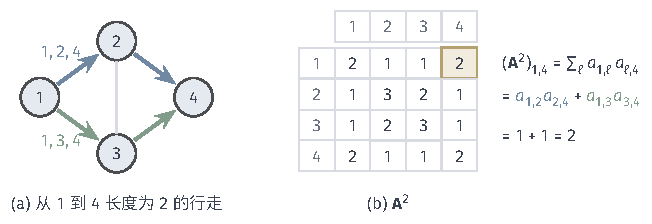
\includegraphics[width=110.352mm]{figures/01-basic-mathematics/04-graphs/tikz/c1-adjacency-square-walks/figure.pdf}
  \caption{邻接矩阵的平方计数长度为$2$的行走。(a)从$1$到$4$的两条行走$(1,2,4)$（蓝色）与$(1,3,4)$（绿色），中间顶点分别是$2$和$3$；(b)贯穿图的$\bm A^2$，黄色条目$(\bm A^2)_{1,4}=2$按中间顶点$\ell$求和，只有$\ell=2,3$的两项非零。}
  \label{fig:graph-conn-adjacency-square}
\end{figure}

这个计数包含重复顶点的行走，不能直接当作路径数或环数使用。例如可以算出$\bm A^3$的对角元依次为$2,4,4,2$，迹为$12$；长度为$3$的闭行走$(v_0,v_1,v_2,v_0)$中相邻两项都不相同（没有自环），于是三个顶点两两相邻，恰好组成一个三角形；而每个三角形可以从$3$个顶点出发、沿$2$个方向绕行，所以三角形个数为$12/6=2$，即$\{1,2,3\}$与$\{2,3,4\}$。更长的闭行走就会混入往返与重复绕行，不能这样简单换算。

带权时，同样的归纳说明$(\bm W^k)_{i,j}$等于所有从$i$到$j$长度为$k$的行走上边权乘积之和。它既不是行走条数，也不是路线长度之和：若边权表示长度，要求的是沿路线相加再取最小，这需要把矩阵乘法中的乘法换成加法、把求和换成取最小值，已经改变了运算规则。路线长度的最优化属于第~\ref{sec:graph-shortest-paths}节。

\subsection{关联矩阵}
\label{sec:graph-conn-incidence-matrix}

邻接矩阵以顶点对为单位，看不出“第几条边”。有些计算需要以边为单位，例如对每条边取出两个端点上的数值作比较。这就要一个行对应顶点、列对应边的矩阵。

\paragraph{定义与逐列核对}
把边编号为$e_1,\ldots,e_m$，并给每条无向边任选一个记录方向，例如把$e_k=\{i,j\}$记为从$i$到$j$。\term{关联矩阵}（incidence matrix）$\bm B\in\mathbb R^{n\times m}$的第$k$列在起点$i$处为$1$、在终点$j$处为$-1$，其余为$0$。有向图直接用弧的方向作为记录方向。

对贯穿图按图~\ref{fig:graph-conn-four-representations}(a)的编号，并统一取“小编号指向大编号”的记录方向，得到
\begin{equation}
\bm B=
\begin{bmatrix}
1&1&0&0&0\\
-1&0&1&1&0\\
0&-1&-1&0&1\\
0&0&0&-1&-1
\end{bmatrix},
\label{eq:graph-conn-running-incidence}
\end{equation}
即图~\ref{fig:graph-conn-four-representations}(d)。逐列读：第$1$列在第$1$行为$1$、第$2$行为$-1$，正是边$e_1=\{1,2\}$；第$5$列在第$3,4$行，正是$e_5=\{3,4\}$。每列恰有两个非零元，且和为$0$；第$i$行的非零元个数等于度$d_i$，例如第$2$行有三个。关联矩阵的每一列与边列表的一条记录一一对应，只是把端点写成了带符号的列向量。

\paragraph{记录方向的选择}
无向边的记录方向是任意选的。把第$k$条边的记录方向反过来，第$k$列整列变号，相当于把$\bm B$右乘一个对角元为$\pm1$的对角矩阵；图本身没有任何改变。所以对无向图，不同的记录方向给出同一张图的不同编码，后续计算若要反映图的性质，结果就不应依赖这一选择。有向图则不同：弧的方向是数据的一部分，反转它就得到另一张有向图。关联矩阵怎样计算每条边两端数值的差，以及它与拉普拉斯矩阵的关系，在第~\ref{sec:graph-vertex-edge-functions}节和第~\ref{sec:graph-laplacian}节展开。

\paragraph{四种表示的比较}
表~\ref{tab:graph-conn-representation-costs}汇总了本节讨论的代价。没有一种表示在所有操作上都最好：逐边处理用边列表，逐点列邻居用邻接表，频繁查询顶点对或做矩阵运算用邻接矩阵，以边为单位的线性计算用关联矩阵。实际程序常同时保存两种表示，额外的存储也应计入代价。

\begin{table}[!htb]
  \centering\small
  \begin{tabular}{@{}lccc@{}}
    \toprule
    表示 & 存储 & 列出$i$的邻居 & 查询$\{i,j\}$是否为边\\
    \midrule
    边列表 & $O(n+m)$ & $O(m)$ & $O(m)$\\
    邻接表 & $O(n+m)$ & $O(d_i)$ & $O(d_i)$\\
    稠密邻接矩阵 & $O(n^2)$ & $O(n)$ & $O(1)$\\
    稠密关联矩阵 & $O(nm)$ & $O(m+d_in)$ & $O(m)$\\
    \bottomrule
  \end{tabular}
  \caption{四种表示的存储与两种基本访问的时间代价，$n$为顶点数，$m$为边数，$d_i$为顶点$i$的度。边列表、邻接表不附加索引；稠密关联矩阵列出邻居时先扫描第$i$行找出$d_i$条邻边，再在每条边的列中找另一个端点。关联矩阵若改用按行、按列都可访问的稀疏存储，存储降为$O(n+m)$，列出邻居的代价与邻接表相当。}
  \label{tab:graph-conn-representation-costs}
\end{table}

\section{图同构}
\label{sec:graph-isomorphism}

顶点的名称只是为了区分顶点而取的。把贯穿图的顶点换一套编号，边集的写法会变，邻接矩阵的行列也会移动，连接结构本身却没有变。比较两张图时，需要一个标准来判断它们是否只差一套名称。本节先用保持邻接的一一对应定义同构，再用第~\ref{sec:prelim-common-matrices}小节的置换矩阵把重编号写成矩阵运算。怎样系统地比较两张图的结构，是第~\ref{sec:graph-wl-refinement}节的内容；这里先把要判定的目标说清楚。

\subsection{图同构的定义}
\label{sec:graph-conn-isomorphism-definition}

图~\ref{fig:graph-conn-isomorphism}(a)是贯穿图$\mathcal G$；(c)的$\mathcal G'$顶点集也是$\{1,2,3,4\}$，边集由$\{1,3\}$、$\{1,4\}$、$\{2,3\}$、$\{2,4\}$、$\{3,4\}$组成，画出来有两条边交叉，看上去与菱形不同。若按(b)的规则$\rho$把$\mathcal G$的顶点改名，$\mathcal G$的五条边依次变为
\[
\begin{gathered}
\{1,2\}\mapsto\{1,3\},\qquad
\{1,3\}\mapsto\{1,4\},\qquad
\{2,3\}\mapsto\{3,4\},\\
\{2,4\}\mapsto\{3,2\},\qquad
\{3,4\}\mapsto\{4,2\},
\end{gathered}
\]
恰好是$\mathcal G'$的全部边；唯一不相邻的一对$\{1,4\}$变为$\{1,2\}$，在$\mathcal G'$中也不相邻。两张图只差一套名称。

\begin{figure}[!htb]
  \centering
  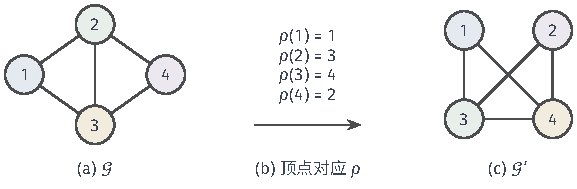
\includegraphics[width=97.688mm]{figures/01-basic-mathematics/04-graphs/tikz/c1-isomorphism-relabeling/figure.pdf}
  \caption{两张同构的图。(a)贯穿图$\mathcal G$；(c)画法与编号都不同的$\mathcal G'$；(b)顶点对应$\rho$。同色顶点互相对应：$\mathcal G$中顶点$i$与$\mathcal G'$中顶点$\rho(i)$颜色相同。逐条核对可见，$\mathcal G$中相邻的顶点对恰好对应$\mathcal G'$中相邻的顶点对。}
  \label{fig:graph-conn-isomorphism}
\end{figure}

\begin{definition}[图同构]
\label{def:graph-conn-isomorphism}
设$\mathcal G=(V,E)$与$\mathcal G'=(V',E')$是无向图。若存在双射$\rho:V\to V'$，使对任意$i,j\in V$都有
\[
\{i,j\}\in E\iff\{\rho(i),\rho(j)\}\in E',
\]
就称$\mathcal G$与$\mathcal G'$\term{同构}（isomorphic），称$\rho$为一个同构映射。
\end{definition}

定义中的双向条件不能减弱为单向。若只要求“$\mathcal G$的边映为$\mathcal G'$的边”，那么把边集为$\{1,2\},\{2,3\}$的路径按恒等映射放进三角形$\{1,2,3\}$也满足要求，但三角形多出了边$\{1,3\}$，两张图的边数不同。反方向的条件保证$\mathcal G'$中不出现$\mathcal G$里没有的连接，即保持不相邻关系。

\paragraph{有向图、加权图与带属性的图}
附加信息越多，同构要保持的东西越多。有向图的同构要求$(i,j)\in E\iff(\rho(i),\rho(j))\in E'$，即保持弧的方向；单向链$1\to2\to3$与$1\to2\leftarrow3$的底层无向图相同，作为有向图却不同构：后者的顶点$2$入度为$2$，前者每个顶点的入度至多为$1$，而有向图的同构映射保持入度。加权图还要求对应的边权相等，$w'_{\rho(i),\rho(j)}=w_{i,j}$；带属性的图则要由问题声明哪些属性必须保持，例如比较两个分子时原子种类必须一致，而原子的编号无关紧要。

\paragraph{用不变量排除同构}
同构映射保持一切由连接结构定义的量：顶点数、边数、每个顶点的度（$\rho$把$i$的邻居一一映为$\rho(i)$的邻居），因而还有全部顶点的度构成的多重集合，以及连通分量的个数、三角形的个数等。这些量称为图的不变量。只要有一个不变量不同，两张图就不同构。例如六个顶点排成一个环，与两个互不相连的三角形相比，顶点数、边数都是$6$，每个顶点的度都是$2$，但前者连通、后者有两个分量，所以不同构。

不变量相同却不足以断定同构。考虑两棵六个顶点的树，边集分别为
\[
\bigl\{\{1,2\},\{1,3\},\{1,4\},\{2,5\},\{3,6\}\bigr\}
\quad\text{与}\quad
\bigl\{\{1,2\},\{1,3\},\{1,4\},\{2,5\},\{5,6\}\bigr\}.
\]
二者都连通、没有三角形，度的多重集合都是$\{3,2,2,1,1,1\}$。但在前一棵树中，唯一的度为$3$的顶点$1$与两个度为$2$的顶点$2,3$相邻；在后一棵树中，顶点$1$只与一个度为$2$的顶点$2$相邻，另一个度为$2$的顶点$5$不是它的邻居。同构映射必须把度为$3$的顶点映到度为$3$的顶点，并保持它的邻居及邻居的度，所以两棵树不同构。这个例子提示，比较“邻居的度”能区分只看度区分不了的图；第~\ref{sec:graph-wl-refinement}节的顶点标记细化正是把这一想法反复执行。逐个尝试全部$n!$个双射虽然总能判定，但随$n$增长得太快，不能作为实用的方法。

\subsection{重编号与置换表示}
\label{sec:graph-conn-relabeling}

当两张图的顶点集都是$\{1,\ldots,n\}$时，同构映射$\rho$就是一个重编号：把顶点$i$改称为$\rho(i)$。重编号以后，邻接矩阵的行和列都要按同样的方式重新排列。第三部分的置换矩阵恰好执行这种重排。

\paragraph{置换共轭}
按第~\ref{sec:prelim-common-matrices}小节，取置换矩阵$\bm P=\begin{bmatrix}\bm e_{\rho(1)}&\cdots&\bm e_{\rho(n)}\end{bmatrix}$，它满足$\bm P\bm e_i=\bm e_{\rho(i)}$。由第~\ref{sec:ls-matrix-operations}小节置换矩阵的乘法规则，左乘$\bm P$把第$i$行移到第$\rho(i)$行；右乘$\bm P^{\top}$相当于对转置后的矩阵左乘$\bm P$，把第$j$列移到第$\rho(j)$列。两者合起来，
\begin{equation}
\bm A'=\bm P\bm A\bm P^{\top},\qquad
a'_{\rho(i),\rho(j)}=a_{i,j}.
\label{eq:graph-conn-relabel}
\end{equation}
第二式说明，原来记录“$i,j$是否相邻”的条目被搬到了新编号$\rho(i),\rho(j)$的位置。因此，$\rho$是$\mathcal G$到$\mathcal G'$的同构映射，当且仅当$\mathcal G'$的邻接矩阵等于$\bm P\bm A\bm P^{\top}$。

\paragraph{核对贯穿图的例子}
对图~\ref{fig:graph-conn-isomorphism}的$\rho$，$\bm P$的各列依次为$\bm e_1,\bm e_3,\bm e_4,\bm e_2$。由式\eqref{eq:graph-conn-running-adjacency}计算得
\[
\bm P=
\begin{bmatrix}
1&0&0&0\\
0&0&0&1\\
0&1&0&0\\
0&0&1&0
\end{bmatrix},\qquad
\bm P\bm A\bm P^{\top}=
\begin{bmatrix}
0&0&1&1\\
0&0&1&1\\
1&1&0&1\\
1&1&1&0
\end{bmatrix}.
\]
右边矩阵的第$1$行在第$3,4$列为$1$，即$N'(1)=\{3,4\}$；第$4$行在第$1,2,3$列为$1$，即$N'(4)=\{1,2,3\}$；各行都与$\mathcal G'$的边集一致。逐个位置看也是如此，例如$a'_{3,2}=a'_{\rho(2),\rho(4)}=a_{2,4}=1$。加权图把$\bm A$换成$\bm W$，同样要求$\bm W'=\bm P\bm W\bm P^{\top}$；允许零权边时，还要同时检验结构掩码$\bm M'=\bm P\bm M\bm P^{\top}$，因为两个顶点之间无边与有一条零权边，权矩阵都是零矩阵。

\paragraph{置换不同于一般换基}
置换矩阵满足$\bm P^{\top}\bm P=\bm I$，所以$\bm P^{\top}=\bm P^{-1}$，式\eqref{eq:graph-conn-relabel}是第~\ref{sec:ls-similarity}小节意义下的相似变换。但反过来，一般的相似变换$\bm S\bm A\bm S^{-1}$不能都解释为重编号。例如对两个顶点一条边的图，$\bm A=\left[\begin{smallmatrix}0&1\\1&0\end{smallmatrix}\right]$，取$\bm S=\left[\begin{smallmatrix}1&1\\0&1\end{smallmatrix}\right]$，得到
\[
\bm S\bm A\bm S^{-1}
=\begin{bmatrix}1&1\\0&1\end{bmatrix}
\begin{bmatrix}0&1\\1&0\end{bmatrix}
\begin{bmatrix}1&-1\\0&1\end{bmatrix}
=\begin{bmatrix}1&0\\1&-1\end{bmatrix},
\]
它不对称，有非零对角元和负条目，已经不是任何简单无向图的邻接矩阵。一般换基会把不同顶点的坐标混合起来，而重编号只搬动位置、不混合数值。相似变换保持特征值，所以同构的图有相同的邻接矩阵特征值；这一事实的用途和局限在第~\ref{chap:graph-spectral}章讨论，这里只确定重编号的精确含义。

\section{本章小结}
\label{sec:graph-objects-summary}

本章围绕三个问题建立了图的基本语言：连接是什么，沿连接能到哪里，结构怎样记录和比较。图$\mathcal G=(V,E)$只记录有限个对象之间的直接连接，与纸上的画法无关。方向、边权和属性各自附加一类信息：方向决定哪些顶点序列可以通行，边权的含义由问题决定，长度相加、容量限制通过量、相似度鼓励两端接近；零权边仍是边，“能否到达”查边集，“累计多少”查边权。子图与诱导子图区分了“任意保留一部分边”和“保留选定顶点之间的全部边”。

沿连接能到哪里，由行走和路径回答。行走允许重复，便于拼接与计数；路径不重复顶点，对应实际路线；任何行走中都含有一条同端点的路径，所以判断可达时两者等价。无向图中可达关系是等价关系，把顶点集唯一地划分为连通分量；有向图中可达不对称，需要区分要求双向到达的强连通与忽略方向的弱连通，前者蕴含后者而反之不然。分隔集、割点和桥刻画了删除顶点或边对连接的影响，判断的依据始终是有没有替代路径：一条边是桥，当且仅当它不在任何环上。树是连通而无环的图，等价于任意两点之间路径唯一；$n$个顶点的树恰有$n-1$条边，连通且有$n-1$条边的图是树，而$n$个顶点、$c$个分量的生成森林恰有$n-c$条边。

同一张图可以用边列表、邻接表、邻接矩阵和关联矩阵记录，四者保存的连接相同，支持的访问和代价不同；邻接矩阵还把图的组合问题与矩阵运算联系起来，$\bm A^k$的条目计数长度为$k$的行走，但其中包含重复顶点。同构用保持邻接与不相邻的双射刻画“只差一套名称”，在矩阵上表现为置换共轭$\bm A'=\bm P\bm A\bm P^{\top}$；度、分量数等不变量可以排除同构，却不足以确认同构。拿到一张图时，可以用这些表示和不变量核对：所关心的结构是否被保留，附加的数值和方向是否交代清楚。

本章定义了连通分量、强连通分量、生成树、有向无环图上的依赖和同构，却还没有给出高效求出它们的方法。第~\ref{chap:graph-traversal}章在邻接表上用广度优先和深度优先遍历实际计算这些对象，用拓扑排序安排有向无环图的次序，并用顶点标记细化比较图的结构；那里的算法输出，仍要按本章的定义与条件检验。


\chapter{图的遍历与结构计算}
\label{chap:graph-traversal}

第~\ref{chap:graph-objects}章定义了可达、连通分量、强连通分量、有向无环图、分隔集和同构，这些定义说明了“什么样的结构算数”，却没有说明面对一张存放在计算机里的图，怎样把它们实际找出来。例如，可达性的定义要求“存在一条路径”，而一张图中的路径数目可以随顶点数指数增长，逐条列举路径并不可行。本章研究的问题是：怎样只沿着邻接关系有组织地访问顶点，就得到距离、分量、依赖次序这些结构，并且知道每一项输出为什么正确、花了多少计算。

第~\ref{sec:graph-bfs}节和第~\ref{sec:graph-dfs}节给出两种基本的访问方式。广度优先遍历用队列由近及远逐层推进，输出最少边数和相应路线；深度优先遍历用栈沿一条分支走到底再退回，输出发现与完成两种次序，并能判断有向环。这两种遍历是后面各节共用的工具。第~\ref{sec:graph-connectivity-computation}节用它们计算无向连通分量和生成森林，引入在不断加边时维护分量的并查集，再用两遍深度优先遍历求出有向图的强连通分量；把每个强分量缩成一点得到的图没有有向环。第~\ref{sec:graph-topological-order}节在这样的无环图上安排依赖次序。第~\ref{sec:graph-separator-blocks}节删除一个给定的顶点集，把图拆成若干共享接口的局部块。第~\ref{sec:graph-wl-refinement}节回到同构问题，用邻域信息反复细化顶点标记，得到不依赖编号的比较手段，并指出它的局限。

本章讨论有限图，输入以邻接表给出（第~\ref{sec:graph-representations}节），默认无自环、无平行边，需要保留边身份时另行说明。记顶点数为$n=|V|$；无向图的边数和有向图的弧数都记为$m$，邻接表中无向边在两端各存一次，有向图默认只存出邻居。复杂度中的$O(n+m)$表示所需基本操作次数不超过$n+m$的常数倍。本章的算法只使用结构上的邻接，不比较边权：生成森林只要求连通、不要求总权最小，广度优先遍历只数边数、不计长度。在给定结构中寻找最小成本或最大流量，是第~\ref{chap:graph-optimization}章的问题。

\section{广度优先遍历}
\label{sec:graph-bfs}

从一个起点出发，哪些顶点能够到达，到达每个顶点最少要走几条边，又该沿哪条路线走？按定义逐条检查路径行不通，因为路径数目可能极多。一个更经济的想法是按距离分层推进：先找出起点的全部邻居，它们离起点一条边；再找出这些邻居的尚未见过的邻居，它们离起点两条边；如此继续，直到没有新顶点出现。本节把这个想法写成算法，说明队列怎样保证“先近后远”，并证明算法记录的层数确实是最少边数。

\subsection{广度优先遍历算法}
\label{sec:graph-trav-bfs-algorithm}

\paragraph{需要记录的状态}
按层推进时，要知道哪些顶点已经见过、哪些顶点等待展开、每个顶点在第几层、它是从哪个顶点过来的。于是对起点$s$维护四项状态：发现标记，表示顶点是否已经被找到；一个先进先出的队列$Q$，存放已经发现、但邻居尚未检查的顶点；边数距离$d(v)$；以及\term{父指针}（parent pointer）$p(v)$，记录$v$是从哪个顶点第一次被找到的。初始时只有$s$被发现，$d(s)=0$，$p(s)$为空，队列为$[s]$；其余顶点未发现，距离记为$+\infty$。这种按层访问的过程称为广度优先遍历，也常称\term{广度优先搜索}（breadth-first search，BFS）。

\begin{algorithm}[广度优先遍历]
\label{alg:graph-trav-bfs}
输入：图$\mathcal G=(V,E)$的邻接表，起点$s\in V$。输出：距离$d(v)$与父指针$p(v)$，$v\in V$。
\begin{enumerate}
  \item 标记$s$为已发现，置$d(s)=0$、$p(s)$为空，令$Q=[s]$；其余顶点未发现，$d(v)=+\infty$。
  \item 当$Q$非空时，取出队首$u$，按邻接表依次读取$u$的邻居$v$（有向图只读出邻居$v\in N^+(u)$）。若$v$未发现，立即标记$v$为已发现，置$d(v)=d(u)+1$、$p(v)=u$，并把$v$放到队尾；若$v$已发现，跳过。
  \item 队列为空时停止。
\end{enumerate}
\end{algorithm}

标记必须在入队时完成，而不是等到出队时。两个已发现的顶点可能共享一个尚未发现的邻居；若出队时才标记，这个邻居会被两个顶点各放入队列一次，距离和父指针也可能被改写。入队即标记保证每个顶点至多入队一次。

\paragraph{贯穿图上的队列轨迹}
在第~\ref{sec:graph-basic-concepts}节的贯穿四点图上，以$1$为起点，并约定按编号从小到大读取邻居。图~\ref{fig:graph-trav-bfs-queue}(b)逐行列出了每次出队后的队列。取出$1$时发现$2,3$，队列变为$[2,3]$；取出$2$时，邻居$1,3$都已发现，只有$4$是新的，队列变为$[3,4]$；取出$3$时，邻居$1,2,4$全部已发现，$4$不会第二次入队；最后取出$4$，队列为空。结果是$d(2)=d(3)=1$、$d(4)=2$，父指针为$p(2)=p(3)=1$、$p(4)=2$。图~\ref{fig:graph-trav-bfs-queue}(a)把各顶点按$d$值分到三层，蓝色箭头就是父指针所指的边。

\begin{figure}[!htb]
  \centering
  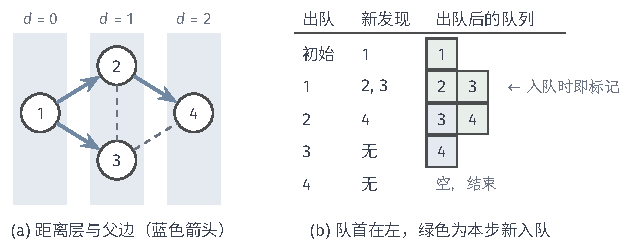
\includegraphics[width=106.7mm]{figures/01-basic-mathematics/04-graphs/tikz/c2-bfs-queue-trace/figure.pdf}
  \caption{贯穿四点图上从顶点$1$出发的广度优先遍历，邻居按编号递增读取。(a)顶点按边数距离$d$分为三层，蓝色箭头是父指针对应的边，虚线是检查过但没有带来新顶点的边。(b)每次出队后的队列，队首在左，绿色格子是这一步新入队的顶点；取出$3$时$4$已在队中，不再重复入队。}
  \label{fig:graph-trav-bfs-queue}
\end{figure}

\paragraph{由父指针恢复路线}
父指针给出的是一条实际路线，而不只是一个距离数值。要得到从$s$到已发现顶点$t$的路线，从$t$出发反复取父指针，直到回到$s$，再把得到的顶点序列反转。在上例中，$4$的父指针是$2$，$2$的父指针是$1$，反转后得到路线$1\to2\to4$，恰有$d(4)=2$条边。父指针总是指向更早发现的顶点，所以沿父指针回溯不会绕圈，一定在有限步内回到$s$。若$t$始终未被发现，即$d(t)=+\infty$，算法应报告$t$从$s$不可达，而不能输出任何路线。

路线并不唯一。若把邻居的读取次序改为先读$3$再读$2$，那么取出$1$后队列为$[3,2]$，$4$会在展开$3$时被发现，父指针变成$p(4)=3$，路线变成$1\to3\to4$。两条路线不同，但边数都是$2$。下面的定理说明，改变同层顶点的处理次序可能改变父指针，却不会改变距离。

\subsection{正确性与计算开销}
\label{sec:graph-trav-bfs-correctness}

\paragraph{为什么首次记录就是最少边数}
记$\operatorname{dist}(s,v)$为从$s$到$v$的路径的最少边数，不可达时为$+\infty$。算法只在顶点第一次被发现时写入$d(v)$，以后不再修改。我们要说明，这个“第一次”恰好发生在最短的距离上。

\begin{theorem}[广度优先遍历的距离]
\label{thm:graph-trav-bfs-distance}
设对有限图$\mathcal G$和起点$s$执行算法~\ref{alg:graph-trav-bfs}。则对每个顶点$v$，$d(v)=\operatorname{dist}(s,v)$；当$v$可达时，沿父指针从$v$回到$s$的路线恰有$d(v)$条边。
\end{theorem}

\begin{proof}
先说明$d(v)$不会小于真实距离。若$d(v)$有限且$v\neq s$，则$d(p(v))=d(v)-1$，沿父指针每退一步距离减一，$d(v)$步后回到$s$。反转这串顶点就得到一条从$s$到$v$、恰有$d(v)$条边的路线，所以$d(v)\geq\operatorname{dist}(s,v)$。

再说明队列中的距离值有一个固定的形状：从队首到队尾不减，且最大值与最小值至多相差$1$。初始队列只有$s$，满足这一点。设某时刻队列中的值为若干个$k$后接若干个$k+1$，取出的队首$u$有$d(u)=k$，新加入的顶点距离都是$k+1$，并放在队尾，形状仍然保持。由此可知，顶点出队时的距离值按时间不减。

最后对$\delta=\operatorname{dist}(s,v)$归纳，证明有限距离的顶点都会被发现且$d(v)\leq\delta$。$\delta=0$时$v=s$。设$\delta\geq1$，并设距离小于$\delta$的顶点都已满足结论。取一条从$s$到$v$的最短路径，记其倒数第二个顶点为$x$，则$\operatorname{dist}(s,x)=\delta-1$，由归纳假设$x$被发现且$d(x)=\delta-1$。$x$入过队，就一定在某一时刻出队并检查邻居$v$。若此时$v$尚未发现，就得到$d(v)=d(x)+1=\delta$；若$v$已经被发现，则发现它的顶点$u$出队不晚于$x$，按上一段的单调性$d(u)\leq d(x)$，于是$d(v)=d(u)+1\leq\delta$。两个方向合起来得到$d(v)=\operatorname{dist}(s,v)$。不可达的顶点没有任何从$s$出发的路线，第一段说明它不可能得到有限的$d$值。
\end{proof}

证明的关键是第二段的队列形状：算法处理第$k$层时，只会首次发现第$k+1$层的顶点；第$k+1$层的顶点全部排在第$k$层之后。倒数第二个顶点$x$比$v$少一层，一定先被展开，因此$v$不可能等到更远的层才被发现。

\paragraph{计算开销}
以邻接表存储时，每个顶点至多入队一次、出队一次；每个顶点出队时把它的邻接表读一遍，因此每条邻接记录只被检查常数次。无向图的邻接记录共$2m$条，有向图的出邻接记录共$m$条，所以总时间为$O(n+m)$。发现标记、距离、父指针和队列各占$O(n)$额外空间。这一结论依赖“列出邻居的代价与度数成正比”。若图以邻接矩阵存储，找出一个顶点的邻居要扫描矩阵的一整行，$n$个顶点共扫描$n^2$个位置，时间变为$O(n^2)$；对稀疏图，这比$O(n+m)$大得多。

\paragraph{最少边数不是最小总长度}
广度优先遍历把每条边都算作一步。边上带有长度时，边数最少的路线不一定总长度最小。图~\ref{fig:graph-trav-bfs-weighted}中，从$s$直接到$t$只需一条边，广度优先遍历就会用这条边记录$t$，但它的长度是$5$；经过$a$的路线多走一条边，总长度却只有$1+1=2$。所以广度优先遍历只解决所有边长相等时的最短路问题。一般边长下的最短路需要比较累计长度，留到第~\ref{sec:graph-shortest-paths}节。

\begin{figure}[!htb]
  \centering
  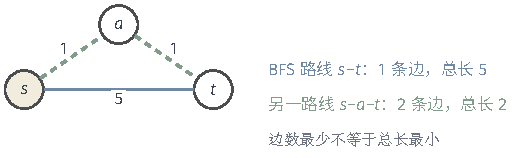
\includegraphics[width=87.8mm]{figures/01-basic-mathematics/04-graphs/tikz/c2-bfs-weighted-counterexample/figure.pdf}
  \caption{带权反例。边旁数字是长度。广度优先遍历从$s$出发时经直接边一步发现$t$（蓝色），这条路线总长$5$；绿色虚线路线$s\text{--}a\text{--}t$多一条边，总长只有$2$。广度优先遍历最小化的是边数，不是总长度。}
  \label{fig:graph-trav-bfs-weighted}
\end{figure}

此外，一次广度优先遍历只覆盖从$s$可达的部分。遍历结束时距离仍为$+\infty$的顶点没有被访问，不能据此断言它们是孤立点，它们之间可能有很多边。要给全图的每个顶点划分连通分量，需要在外层不断换新的起点重新启动，这是第~\ref{sec:graph-connectivity-computation}节的内容。

\subsection{多源广度优先遍历}
\label{sec:graph-trav-multi-source-bfs}

\paragraph{从一组起点同时出发}
有时关心的不是离某一个起点有多远，而是离一组起点中最近的那个有多远。例如在网格上放置若干个种子，问每个格子离最近的种子几步。给定起点集合$S\subseteq V$，定义
\[
\operatorname{dist}(S,v)=\min_{s\in S}\operatorname{dist}(s,v),
\]
空集上的最小值约定为$+\infty$。做法是把$S$中所有顶点同时作为第$0$层：初始时它们都被标记、距离为$0$、父指针为空，并按任意次序全部放入队列，此后完全按算法~\ref{alg:graph-trav-bfs}执行。这称为\term{多源广度优先遍历}（multi-source breadth-first search）。

为什么这样得到的是到最近起点的距离？设想添加一个新顶点$s^*$，从它向$S$中每个顶点连一条边（有向图中连弧$s^*\to s$）。在新图中，任一顶点$v\notin\{s^*\}$满足$\operatorname{dist}(s^*,v)=1+\operatorname{dist}(S,v)$，因为从$s^*$出发的路线第一步必然进入$S$中的某个点。从$s^*$做普通广度优先遍历，第一次出队就把$S$中所有顶点以距离$1$放入队列，此后的过程与多源版本完全相同，只是所有距离多了$1$。由定理~\ref{thm:graph-trav-bfs-distance}即得多源版本输出$\operatorname{dist}(S,v)$，而且沿父指针回溯会停在某个起点上，它就是离$v$最近的起点之一。

\paragraph{网格上的种子传播}
图~\ref{fig:graph-trav-multi-source}是一个$3\times5$网格，相邻格子以上下左右相连，中间一个格子不属于图。两个起点放在左上角和右下角，每个格子中的数字是它到较近起点的边数。例如第一行第四个格子离左上角$3$步、离右下角$3$步，记为$3$；第一行最右的格子离右下角只有$2$步，记为$2$。若只从左上角出发，右下角的格子距离为$6$。

\begin{figure}[!htb]
  \centering
  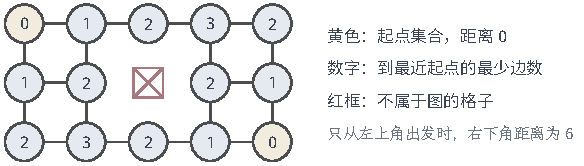
\includegraphics[width=99.0mm]{figures/01-basic-mathematics/04-graphs/tikz/c2-multi-source-bfs/figure.pdf}
  \caption{$3\times5$网格上的多源广度优先遍历。网格以上下左右相邻连边，红框格子不属于图；两个黄色起点同时作为第$0$层。每个顶点中的数字是到较近起点的最少边数，所有距离由一次遍历得到。}
  \label{fig:graph-trav-multi-source}
\end{figure}

\paragraph{与逐个起点遍历的区别}
多源遍历与“对每个起点各做一次广度优先遍历”回答的是不同问题。后者得到$|S|$组距离，能说出$v$到每一个起点各有多远，需要$O(|S|(n+m))$时间；多源遍历只给出到最近起点的距离及对应的起点，一次遍历只需$O(n+m)$时间。若$S$为空，队列一开始就为空，所有顶点保持未发现，输出的可达集为空集，这与$\operatorname{dist}(\varnothing,v)=+\infty$的约定一致。图像中从种子出发的区域生长是这一机制的典型用途；判断哪些像素属于前景、怎样选择邻接规则等完整处理留到应用部分。

\section{深度优先遍历}
\label{sec:graph-dfs}

广度优先遍历同时推进许多条路线，每条只走一步。另一种访问方式是只盯住一条路线：从当前顶点走向一个尚未见过的邻居，再从那里继续往前，直到无路可走才退回上一个顶点，改走它的下一个邻居。走迷宫时用左手扶墙一路前进、碰到死路再折回，就是这种方式。它天然地维持着“当前正在走的这条分支”，因而能判断沿当前分支是否绕回了自己，也能记录每个顶点何时把所有出路都探完。本节建立这一过程，并说明这两条信息分别有什么用。

\subsection{栈与递归访问}
\label{sec:graph-trav-dfs-stack}

\paragraph{三种状态与栈帧}
沿分支前进时，一个顶点经历三个阶段：尚未被走到，称为未发现；已经走到、但它的邻居还没有检查完，称为处理中；邻居全部检查完毕、不会再从它出发，称为已完成。区分后两种状态是必要的，因为“已经见过”并不等于“已经处理完”。处于处理中的顶点恰好构成从本次起点到当前位置的一条分支，用一个后进先出的栈保存：栈底是起点，栈顶是当前顶点。

只记住栈中的顶点还不够。退回到某个顶点时，需要接着检查它的下一个邻居，而不是从头再来。因此栈中的每一帧保存一个顶点$u$，以及$u$的邻接表中下一条待检查记录的位置。另外用父指针$p(v)$记录$v$是从哪个顶点走过来的。这种访问方式称为深度优先遍历，也常称\term{深度优先搜索}（depth-first search，DFS）。

\begin{algorithm}[深度优先遍历（显式栈）]
\label{alg:graph-trav-dfs}
输入：图$\mathcal G=(V,E)$的邻接表。输出：父指针、每个顶点的发现时刻$d(v)$与完成时刻$f(v)$。
\begin{enumerate}
  \item 所有顶点置为未发现，时钟$t=0$。按某个固定次序扫描顶点；每遇到一个未发现的顶点$r$，令$p(r)$为空，执行下面两步。
  \item 发现$r$：$t\gets t+1$，$d(r)=t$，$r$改为处理中，把帧$(r,\text{邻接表起点})$压入栈。
  \item 当栈非空时，看栈顶帧$(u,\text{位置})$。若$u$还有未检查的邻居，读取下一个邻居$v$（有向图只读出邻居），并把位置后移一格：$v$未发现时，置$p(v)=u$，$t\gets t+1$，$d(v)=t$，$v$改为处理中并压入新帧；$v$处于处理中或已完成时，不压栈，继续下一轮。若$u$的邻居已全部检查，则$t\gets t+1$，$f(u)=t$，$u$改为已完成并弹出栈顶帧。
\end{enumerate}
\end{algorithm}

用递归写，同样的过程更短：访问$u$时先记发现时刻，然后对每个未发现的邻居$v$置$p(v)=u$并递归访问$v$，所有邻居处理完后记完成时刻。递归调用时，程序运行时会自动保存“$u$检查到了第几个邻居”，这正是显式栈中每一帧记录的位置。两种写法的访问次序完全一样。

\paragraph{完整执行过程}
图~\ref{fig:graph-trav-dfs-stack}(a)是一个有分支的有向图，弧为$1\to2$、$1\to5$、$2\to3$、$2\to4$、$5\to4$。从$1$出发并按编号读取出邻居：发现$1$，再发现$2$，再发现$3$；$3$没有出邻居，于是完成$3$并弹栈，回到$2$。$2$的下一个出邻居$4$未发现，压栈；$4$也没有出邻居，完成后回到$2$，此时$2$的邻居已检查完，完成$2$。回到$1$，它的下一个出邻居$5$未发现，压栈；$5$唯一的出邻居$4$已经完成，不再压栈，$5$随即完成；最后完成$1$，栈变空。图~\ref{fig:graph-trav-dfs-stack}(b)画出了每个事件之后的栈，黄色格子是栈顶。

\begin{figure}[!htb]
  \centering
  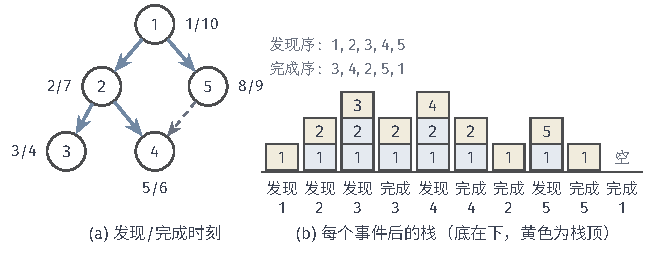
\includegraphics[width=109.8mm]{figures/01-basic-mathematics/04-graphs/tikz/c2-dfs-stack-trace/figure.pdf}
  \caption{有向图$1\to2$、$1\to5$、$2\to3$、$2\to4$、$5\to4$上从$1$出发的深度优先遍历，出邻居按编号读取。(a)顶点旁的“$d/f$”是发现时刻与完成时刻，蓝色箭头是父指针对应的弧，虚线弧$5\to4$检查时$4$已完成。(b)十个事件后的栈，底在下、栈顶为黄色；栈高上升对应发现，下降对应完成。}
  \label{fig:graph-trav-dfs-stack}
\end{figure}

若栈空时仍有未发现的顶点，算法回到第一步，从下一个未发现顶点重新开始。已经完成的顶点保持原状态，不会被重新访问。这样，整次执行把每个顶点恰好发现一次、完成一次；父指针把顶点组织成若干棵有根树，称为深度优先森林。只在发现时处理顶点，得不到“何时探完”的信息，因此完成事件要单独记录，下一小节会看到它的用处。

\paragraph{计算开销}
每个顶点恰好压栈一次、弹栈一次；每一帧的位置只向后移动，所以每条邻接记录恰好被读取一次。邻接表下总时间为$O(n+m)$，状态、时刻、父指针和栈占$O(n)$额外空间。栈的深度等于当前分支上的顶点数，最坏可达$n$：在一条长链$1\to2\to\cdots\to n$上，栈会一直增长到装下全部顶点。递归实现时，这意味着递归深度也是$n$，可能超出程序运行环境允许的调用深度；显式栈把这部分存储放在普通数组中，避免这一问题。

\subsection{发现次序与完成次序}
\label{sec:graph-trav-dfs-orders}

\paragraph{两种次序}
按发现时刻从小到大排列顶点，得到\term{发现次序}（discovery order）；按完成时刻排列，得到\term{完成次序}（finishing order）。在图~\ref{fig:graph-trav-dfs-stack}中，发现次序是$1,2,3,4,5$，完成次序是$3,4,2,5,1$。两种次序的差别来自栈的结构：一个顶点被发现之后，在它弹栈之前压入的所有顶点都位于它上方，必须先弹出。所以一个顶点的后代全部先于它完成，而它自己最后完成；$2$的后代$3,4$先完成，然后才轮到$2$。

下面两个引理把这一观察写准确。第一个说明时刻区间怎样嵌套，第二个说明哪些顶点一定会成为后代；第~\ref{sec:graph-connectivity-computation}节计算强连通分量、第~\ref{sec:graph-topological-order}节构造拓扑次序时都要用到它们。

\begin{lemma}[时刻区间的嵌套]
\label{lem:graph-trav-dfs-nesting}
在一次完整的深度优先遍历中，若顶点$v$在$u$处于处理中时被发现，即$d(u)<d(v)<f(u)$，则$v$是$u$在深度优先森林中的后代，且$f(v)<f(u)$。
\end{lemma}

\begin{proof}
$v$被发现时压入栈，位于$u$的上方，因为此时$u$仍在栈中。栈后进先出，$v$必须在$u$之前弹出，所以$f(v)<f(u)$。另外，$v$的父指针指向发现它时的栈顶，这个栈顶要么是$u$，要么是在$u$之后压入的顶点；对后者重复同样的推理，父指针链只会经过$u$上方的顶点，最终到达$u$。因此$v$是$u$的后代。
\end{proof}

\begin{lemma}[未发现路径]
\label{lem:graph-trav-white-path}
若在时刻$d(u)$存在一条从$u$到$v$的路径（有向图中沿弧方向），路径上除$u$以外的顶点此时都未发现，则$v$最终成为$u$的后代，从而$f(v)<f(u)$。
\end{lemma}

\begin{proof}
假设结论不成立，在路径上取第一个不成为$u$后代的顶点$w$，记它在路径上的前一个顶点为$x$。$x$是$u$本身或$u$的后代，所以$f(x)\leq f(u)$。$x$在完成之前要检查弧$x\to w$，因此$w$在$f(x)$之前已被发现；而按假设$w$在$d(u)$时尚未发现，所以$d(u)<d(w)<f(x)\leq f(u)$。由引理~\ref{lem:graph-trav-dfs-nesting}，$w$是$u$的后代，矛盾。
\end{proof}

\paragraph{共享后继：发现次序不能代替完成次序}
设图~\ref{fig:graph-trav-dfs-stack}中的弧表示依赖，$i\to j$意味着$i$要排在$j$之前。顶点$4$同时是$2$和$5$的后继。若按发现次序$1,2,3,4,5$安排，$5$排在$4$之后，违反了弧$5\to4$：发现$4$时走的是经过$2$的分支，发现次序完全没有反映$5$也指向它。完成次序则不同。$4$在$5$之前就已完成，反转完成次序得到$1,5,2,4,3$，逐条检查五条弧都是起点在前。第~\ref{sec:graph-trav-dfs-toposort}节会证明，在无环图中这一做法总是成立。

\paragraph{父路径一般不是最短路线}
深度优先遍历的父指针同样给出从根到每个顶点的路线，但它反映的是“沿哪条分支先走到”，与距离无关。在贯穿四点图上从$1$出发、按编号读取邻居：$1$走到$2$，$2$的第一个未发现邻居是$3$，$3$的未发现邻居是$4$，于是父路径为$1\to2\to3\to4$，有三条边；而$1\to2\to4$只需两条边，$1$与$3$甚至直接相邻。需要最少边数时，应使用广度优先遍历。

\subsection{环的检测与恢复}
\label{sec:graph-trav-cycle-detection}

\paragraph{有向图：指向栈内顶点的弧}
处理中的顶点构成当前分支，并且父指针已经把它们按先后串成一条有向路径。若在检查栈顶$u$的出邻居时遇到弧$u\to v$，而$v$也处于处理中，那么沿父指针从$u$往回走一定会到达$v$，这段路径与弧$u\to v$合起来就是一个有向环。这样的弧称为\term{回边}（back edge）。图~\ref{fig:graph-trav-cycle-detection}(a)中，栈内依次是$1,2,3$，检查$3\to1$时$1$仍在栈中，沿父指针$3\to2\to1$回溯，再补上$3\to1$，得到有向环$1\to2\to3\to1$。

指向已完成顶点的弧不能这样处理。图~\ref{fig:graph-trav-cycle-detection}(b)中先走$1\to2$，$2$没有出邻居而完成；回到$1$后走到$3$，检查$3\to2$时$2$已完成。$2$已经不在当前分支上，弧$3\to2$无法与当前分支拼成环。本例中从$2$出发也回不到$3$（否则由引理~\ref{lem:graph-trav-white-path}，$3$会在$2$完成之前就被发现），图中确实没有环。一般地，指向已完成顶点的弧本身不提供成环的证据；图中若另有环，下面的定理保证遍历会在别处遇到回边。只看“是否已经访问过”会把这种情形误判为环，这正是要区分处理中与已完成的原因。

\begin{figure}[!htb]
  \centering
  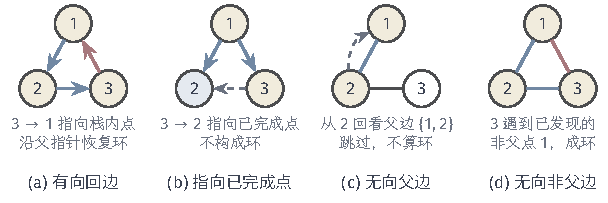
\includegraphics[width=102.9mm]{figures/01-basic-mathematics/04-graphs/tikz/c2-dfs-cycle-detection/figure.pdf}
  \caption{深度优先遍历中环的判断。黄色为处理中（在栈内）的顶点，蓝色填充为已完成顶点，蓝色粗线为父指针对应的边。(a)有向图中$3\to1$指向栈内顶点，构成回边，沿父指针恢复出环；(b)$3\to2$指向已完成顶点，不构成环；(c)无向图中从$2$回看父边$\{1,2\}$，这是同一条边的反向查看，应当跳过；(d)无向三角形中$3$遇到已发现、但不经父边相连的顶点$1$，构成环（红色）。}
  \label{fig:graph-trav-cycle-detection}
\end{figure}

\begin{theorem}[有向环的判定]
\label{thm:graph-trav-directed-cycle}
有限有向图含有向环，当且仅当对它的一次完整深度优先遍历中出现回边。出现回边$u\to v$时，父指针链$v\to\cdots\to u$加上弧$u\to v$就是一个有向环。
\end{theorem}

\begin{proof}
充分性已在上面说明：$v$处于处理中且$u$是当前栈顶，$u$在$v$上方，由引理~\ref{lem:graph-trav-dfs-nesting}$u$是$v$的后代，父指针链给出从$v$到$u$的有向路径。

必要性。设图含有向环，在环上取最先被发现的顶点$v$，记环上指向$v$的弧为$u\to v$。在时刻$d(v)$，环上其余顶点都未发现，沿环从$v$走到$u$的路径满足引理~\ref{lem:graph-trav-white-path}的条件，所以$u$成为$v$的后代，$d(v)<d(u)<f(u)<f(v)$。$u$在完成之前要检查弧$u\to v$，那时$v$尚未完成，仍处于处理中，因此$u\to v$是一条回边。
\end{proof}

\paragraph{无向图：跳过实际的父边}
无向图中每条边在两端的邻接表里各出现一次。从$u$走到$v$之后，$v$检查邻居时会再次看到$u$，这只是同一条边的反向记录，不是新的路线。若把它当作“遇到已发现顶点”，任何一条边都会被误判为环，如图~\ref{fig:graph-trav-cycle-detection}(c)。因此规则是：检查$u$的一条邻接记录$e=\{u,w\}$时，若$e$就是使$u$被发现的父边，跳过；否则只要$w$已经被发现，就报告存在环。图~\ref{fig:graph-trav-cycle-detection}(d)中，$3$经父边与$2$相连，它看到的$1$已被发现、且不经父边相连，于是$1\text{--}2\text{--}3\text{--}1$是一个环。允许平行边时，要按边的身份跳过，只跳过实际作为父边的那一条；两点之间的另一条平行边会与父边构成长度为$2$的环。

这一规则在两个方向上都可靠。若整次遍历从未报告，每条边在两端被检查时，要么发现了新顶点而成为父边，要么正是父边的反向记录，所以所有边都是父边，图就是深度优先森林本身，没有环。反过来，考察第一次报告时的边$e=\{u,w\}$，可以说明$w$此时一定在栈中。假设$w$已完成。$w$完成之前检查过$e$：若那时$u$未发现，$u$会成为$w$的后代并先于$w$完成，与$u$此刻仍在处理相矛盾；若那时$u$已发现，那次检查本身就该报告，除非$e$是$w$的父边，而这意味着$u$当初已经通过$e$发现了$w$，不会现在才第一次读到$e$。于是$w$是栈中位于$u$下方的祖先，父指针链从$w$到$u$再加上$e$构成一个环；由于$e$不是$u$的父边，在简单图中这个环至少有三个顶点。算法既给出了“有环”的结论，也给出了这个环本身，可以直接核对。

\section{连通结构的计算}
\label{sec:graph-connectivity-computation}

第~\ref{sec:graph-connectivity-separation}节把顶点按相互可达划分为连通分量或强连通分量，第~\ref{sec:graph-trees-forests}节说明每个无向分量都有生成树。这些都是存在性的定义。本节把它们算出来：先用遍历给无向图的每个分量编号并抽出生成森林；再处理边不断加入、分量不断合并的情形，引入并查集；最后计算有向图的强连通分量。后一个问题不能简单地重复启动遍历，因为从一个顶点出发能到达的范围，往往大于与它相互可达的范围。

\subsection{连通分量与生成森林}
\label{sec:graph-trav-components-forest}

\paragraph{外层扫描与分量编号}
一次广度或深度优先遍历恰好找出起点所在分量的全部顶点：在无向图中，可达关系是对称的，从$r$可达的顶点就是与$r$相互连通的顶点。要给所有分量编号，只需在外面再套一层扫描。

\begin{algorithm}[无向连通分量编号]
\label{alg:graph-trav-components}
输入：无向图的邻接表。输出：每个顶点的分量编号$\operatorname{comp}(v)$，以及分量数$c$。
\begin{enumerate}
  \item 所有顶点置为未标记，$c=0$。
  \item 按任意固定次序扫描顶点。遇到未标记的顶点$r$时，令$c\gets c+1$，从$r$启动一次广度（或深度）优先遍历，把这次新发现的每个顶点$v$标记为$\operatorname{comp}(v)=c$。已经标记的顶点不再作为起点，也不清除旧编号。
  \item 扫描完全部顶点后输出。
\end{enumerate}
\end{algorithm}

外层扫描必须覆盖全部顶点，否则没有边的孤立点永远不会被任何遍历发现，也就得不到编号。图~\ref{fig:graph-trav-components-forest}中的图由贯穿四点图、一条边$\{5,6\}$和孤立点$7$组成。按编号扫描，从$1$出发的遍历标出$\{1,2,3,4\}$；扫描到$2,3,4$时它们已有编号，跳过；从$5$出发标出$\{5,6\}$；最后$7$自成一个分量。若改变扫描次序，例如先扫描$7$，编号的数值会变，但哪些顶点被分到一起不会变，因为分量本身由图决定。各次遍历合起来把每个顶点和每条邻接记录处理常数次，总时间为$O(n+m)$。

\paragraph{保留发现父边得到生成森林}
遍历时每个新顶点都是经某条边第一次被发现的。把这些父边$\{p(v),v\}$全部保留下来，重复遇到已发现顶点的边一律不加，就得到原图的一个生成森林。

\begin{theorem}[发现父边构成生成森林]
\label{thm:graph-trav-parent-forest}
设对无向图$\mathcal G$执行算法~\ref{alg:graph-trav-components}，并保留所有父边。则这些父边与全部顶点组成$\mathcal G$的一个生成森林，它在每个分量上是一棵生成树，边数为$n-c$。
\end{theorem}

\begin{proof}
每个非起点顶点恰有一条父边，父边的另一端是更早发现的顶点；起点没有父边。于是父边共$n-c$条。

再说明父边不成环。假设某些父边构成一个环，取环上最晚发现的顶点$v$。$v$在环上有两条边，另两端都比$v$早发现。但与$v$相连的父边中，只有$v$自己的父边通向更早发现的顶点，其余父边都是$v$的子顶点的父边，另一端比$v$晚发现。矛盾。

最后，每次遍历从起点出发，沿父指针可以从任何新发现的顶点回到起点，所以每个分量内的父边是连通的。连通、无环、覆盖分量的全部顶点，就是该分量的生成树。
\end{proof}

\begin{figure}[!htb]
  \centering
  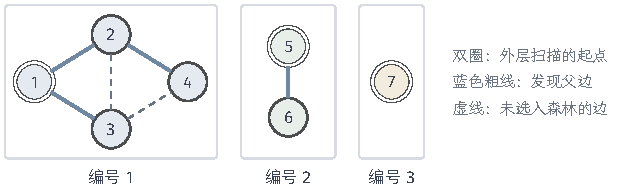
\includegraphics[width=104.8mm]{figures/01-basic-mathematics/04-graphs/tikz/c2-components-spanning-forest/figure.pdf}
  \caption{外层扫描与生成森林。图由贯穿四点图、边$\{5,6\}$和孤立点$7$组成，按编号扫描、每次启动广度优先遍历。三个分量分别获得编号$1,2,3$；双圈是每次遍历的起点，蓝色粗线是保留的父边，共$4=7-3$条，虚线边被检查过但未选入森林。}
  \label{fig:graph-trav-components-forest}
\end{figure}

\paragraph{生成森林丢掉了什么}
图~\ref{fig:graph-trav-components-forest}中第一个分量保留了$\{1,2\}$、$\{1,3\}$、$\{2,4\}$，舍弃了$\{2,3\}$和$\{3,4\}$。生成森林保留了“谁和谁连通”，却不保留其他结构。原图中$3$与$4$直接相邻，在森林中却要走$3\to1\to2\to4$三步；原图没有割点，删去任何一个顶点后其余顶点仍然连通，而在森林中删去$1$或$2$都会把树断开。此外，算法只关心是否连通，边上若有权重，选出的边也没有任何总权最小的保证；在所有生成树中选总权最小的一棵，是第~\ref{sec:graph-minimum-spanning-tree}节的问题。

\subsection{增量连通性与并查集}
\label{sec:graph-trav-union-find}

\paragraph{边不断加入时的分量}
设顶点集固定，边一条一条地加入，每加入一条边后都要回答“两个给定顶点现在是否连通”。每次都重新遍历全图需要$O(n+m)$时间，太浪费。注意加入边$\{u,v\}$对分量的影响很简单：若$u,v$原来已在同一分量，分量不变；否则把两个分量合并成一个。分量构成顶点集的一个划分，加边只会合并其中的两块，不会拆分。于是需要一种数据结构，维护若干互不相交的集合，支持两种操作：$\operatorname{find}(v)$返回$v$所在集合的代表元，两顶点连通当且仅当它们的代表元相同；$\operatorname{union}(u,v)$把$u$和$v$所在的两个集合合并。这种数据结构称为\term{并查集}（union-find），也称不相交集合结构。

\paragraph{父指针树}
并查集把每个集合存成一棵有根树：每个元素保存一个父指针，根的父指针指向自己，根就是集合的代表元。$\operatorname{find}(v)$从$v$出发沿父指针一直走到根；$\operatorname{union}(u,v)$先求出两个根，若不同，就把一个根的父指针改为指向另一个根。这里的父指针只表示“属于同一集合”，与原图的边没有关系：合并$\{1,3\}$时，可能是$3$的根被接到$1$的根下，而原图中这两个根之间未必有边。需要输出原图中的连接时，应另外保存实际加入的边。

\paragraph{按大小合并与路径压缩}
若合并时随意选择谁接到谁下面，树可能退化成一条长链，$\operatorname{find}$要走很多步。两条规则可以避免这一点。

\begin{algorithm}[并查集的两种操作]
\label{alg:graph-trav-union-find}
状态：每个元素$v$的父指针$\operatorname{parent}(v)$，每个根$r$所在集合的大小$\operatorname{size}(r)$。初始时每个元素自成一个集合，$\operatorname{parent}(v)=v$，$\operatorname{size}(v)=1$。
\begin{enumerate}
  \item $\operatorname{find}(v)$：沿父指针从$v$走到根$r$；然后把这条路上经过的每个元素的父指针都直接改为$r$（路径压缩）；返回$r$。
  \item $\operatorname{union}(u,v)$：求$r_u=\operatorname{find}(u)$、$r_v=\operatorname{find}(v)$。若$r_u=r_v$，不做任何事。否则把较小集合的根接到较大集合的根下，大小相同时把$r_v$接到$r_u$下（按大小合并），并把新根的大小更新为两者之和。
\end{enumerate}
\end{algorithm}

图~\ref{fig:graph-trav-union-find}按边序列$\{1,2\}$、$\{3,4\}$、$\{1,3\}$、$\{5,6\}$、$\{4,6\}$追踪这些操作。前两次合并各把一个单点接到另一个单点下，得到$\{1,2\}$与$\{3,4\}$，此时还有单点集合$\{5\}$、$\{6\}$。合并$\{1,3\}$时两个集合大小都是$2$，按约定把根$3$接到根$1$下，$4$的深度变为$2$。之后若查询$\operatorname{find}(4)$，沿$4\to3\to1$找到根$1$，路径压缩把$4$的父指针直接改为$1$，下次查询只需一步。合并$\{5,6\}$得到大小为$2$的集合；处理$\{4,6\}$时，$4$所在集合大小为$4$、$6$所在集合大小为$2$，于是根$5$接到根$1$下，全部六个元素属于同一集合。每一步后的集合划分都与“已加入的边构成的图的连通分量”一致。

\begin{figure}[!htb]
  \centering
  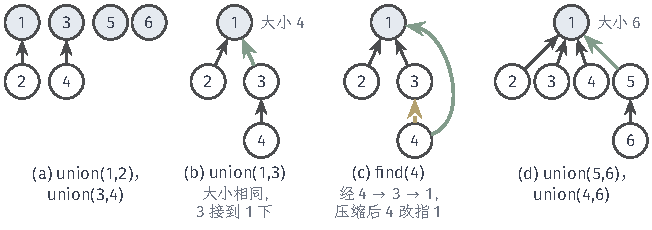
\includegraphics[width=110.5mm]{figures/01-basic-mathematics/04-graphs/tikz/c2-union-find/figure.pdf}
  \caption{并查集的父指针树，箭头由元素指向其父指针，蓝色填充为根。(a)合并$\{1,2\}$、$\{3,4\}$后；(b)合并两个大小为$2$的集合，按约定把根$3$接到根$1$下（绿色箭头）；(c)查询$\operatorname{find}(4)$经过$4\to3\to1$（黄色虚线是原父指针），路径压缩后$4$直接指向根$1$；(d)合并$\{5,6\}$后再处理$\{4,6\}$，较小集合的根$5$接到较大集合的根$1$下。}
  \label{fig:graph-trav-union-find}
\end{figure}

\paragraph{树高与操作开销}
按大小合并能保证树不会太高。

\begin{theorem}[按大小合并的树高]
\label{thm:graph-trav-union-by-size}
只使用按大小合并（无论是否路径压缩）时，任一元素到根的路径长度不超过$\log_2 n$，其中$n$是元素总数。
\end{theorem}

\begin{proof}
先不考虑路径压缩。一个元素的深度只在它所在的根被接到另一个根下面时增加$1$；按规则，被接的那一侧不大于另一侧，所以合并后该元素所在集合的大小至少是原来的两倍。集合大小从$1$开始，不超过$n$，至多翻倍$\log_2 n$次，深度也就至多为$\log_2 n$。路径压缩只把元素的父指针改为它的某个祖先，只会让深度变小，不影响这个上界。
\end{proof}

因此每次$\operatorname{find}$和$\operatorname{union}$都只需$O(\log n)$时间，存储为$O(n)$。路径压缩使反复查询同一区域变得更快。可以证明，两条规则同时使用时，任意$k$次操作的总时间为$O(k\,\alpha(n))$，其中$\alpha$是增长极慢的反Ackermann函数，对任何实际规模的$n$都不超过$4$；这一摊还分析较长，这里不展开，使用时只需记住每次操作的平均代价几乎是常数。

\paragraph{适用范围}
并查集适合“只加边、不删边”的情形。第~\ref{sec:graph-minimum-spanning-tree}节的Kruskal算法按边权从小到大考虑每条边，需要判断加入这条边是否会成环，也就是判断两个端点是否已在同一分量，正好用并查集完成。删除一条边可能把一个分量拆成两个，而并查集的合并无法撤销，所以它不能直接维护任意删边后的分量。在图像中给相连的像素区域编号时，也常先给像素临时标号、再用并查集合并相遇的标号，具体扫描方式留到应用部分。

\subsection{强连通分量与缩点}
\label{sec:graph-trav-scc}

\paragraph{一次搜索为什么不够}
在有向图中，从顶点$v$出发的一次遍历找到的是$v$能到达的全部顶点，而$v$所在的强连通分量要求双向可达。图~\ref{fig:graph-trav-kosaraju}(a)中，从$1$出发的深度优先遍历依次发现$1,2,3,4$，但$3,4$回不到$1$，$1$所在的强连通分量只是$\{1,2\}$。一般地，$v$所在的强分量等于“从$v$可达的顶点”与“能到达$v$的顶点”的交集；后者可以在把所有弧反向后的图上从$v$遍历得到。对每个顶点都这样做两次遍历需要$O(n(n+m))$时间。下面的算法只用两遍深度优先遍历，在$O(n+m)$时间内求出全部强连通分量。

\paragraph{两遍深度优先遍历}
把有向图$\mathcal G$的每条弧$u\to v$改为$v\to u$，得到\term{反向图}（reverse graph）$\mathcal G^{\mathrm{rev}}$。$\mathcal G$与$\mathcal G^{\mathrm{rev}}$的强连通分量相同，因为相互可达的两个顶点在弧全部反向后仍然相互可达。算法的第一遍在原图上计算完成时刻，第二遍在反向图上按完成时刻从大到小选择起点。这一方法称为\term{Kosaraju算法}（Kosaraju's algorithm）。

\begin{algorithm}[Kosaraju强连通分量算法]
\label{alg:graph-trav-kosaraju}
输入：有向图$\mathcal G=(V,E)$的出邻接表。输出：每个顶点所属强连通分量的编号。
\begin{enumerate}
  \item 在$\mathcal G$上执行完整的深度优先遍历（算法~\ref{alg:graph-trav-dfs}），覆盖全部顶点，记录完成次序。
  \item 扫描出邻接表，构造反向图$\mathcal G^{\mathrm{rev}}$的出邻接表，即原图的入邻接表。
  \item 所有顶点置为未标记。按完成时刻从大到小扫描顶点；遇到未标记的顶点$r$时，开始一个新分量，在$\mathcal G^{\mathrm{rev}}$上从$r$遍历（广度或深度优先均可），只进入未标记的顶点，把这次到达的顶点全部标为这个分量。
\end{enumerate}
\end{algorithm}

\paragraph{在三个强分量组成的图上追踪}
图~\ref{fig:graph-trav-kosaraju}的有向图有七个顶点，弧为$1\to2$、$2\to1$、$2\to3$、$3\to4$、$4\to3$、$5\to6$、$6\to4$、$6\to7$、$7\to1$、$7\to5$。它的强连通分量是$\{5,6,7\}$、$\{1,2\}$和$\{3,4\}$，分量之间只有单向的弧。

第一遍按编号选择起点、按编号读取出邻居。从$1$出发，依次发现$1,2,3,4$；$4$的出邻居$3$在栈中，$4$完成，随后$3,2,1$依次完成，完成时刻为$f(4)=5$、$f(3)=6$、$f(2)=7$、$f(1)=8$。接着从$5$重新出发，发现$5,6$；$6$的出邻居$4$已完成，跳过，再发现$7$；$7$的出邻居$1$已完成、$5$在栈中，于是$7,6,5$依次完成，$f(7)=12$、$f(6)=13$、$f(5)=14$。完成次序为$4,3,2,1,7,6,5$，见图~\ref{fig:graph-trav-kosaraju}(a)。

第二遍按完成时刻从大到小，即$5,6,7,1,2,3,4$选择起点，在反向图上遍历，见图~\ref{fig:graph-trav-kosaraju}(b)。从$5$出发，反向弧把它引向$7$，再引向$6$；$\{5,6,7\}$中没有反向弧通往别处，于是得到第一个分量$\{5,6,7\}$。下一个未标记的是$1$：反向弧$1\to2$、$1\to7$中$7$已标记，只进入$2$，得到$\{1,2\}$。最后从$3$出发，反向弧$3\to2$通往已标记的$2$，只进入$4$，得到$\{3,4\}$。每次遍历恰好停在一个强分量的边界上。若第二遍在原图而不是反向图上从$5$遍历，会经$6\to4$、$7\to1$走进另外两个分量，所以反向这一步不可省略。

\begin{figure*}[!htb]
  \centering
  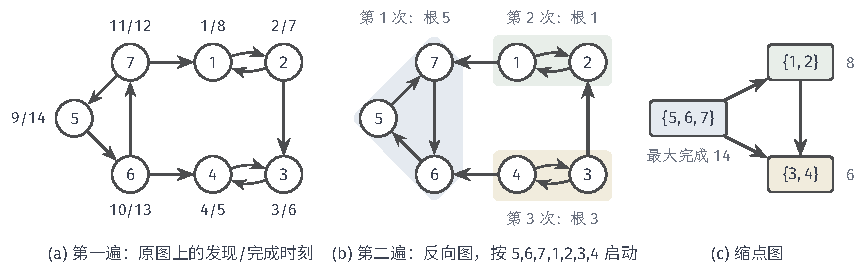
\includegraphics[width=146.5mm]{figures/01-basic-mathematics/04-graphs/tikz/c2-kosaraju-condensation/figure.pdf}
  \caption{Kosaraju算法的两遍过程与缩点图。(a)原图上按编号重启的深度优先遍历，顶点旁为发现/完成时刻；粗箭头是连接不同强分量的弧。(b)反向图上按完成时刻从大到小（$5,6,7,1,2,3,4$）选择起点，三次遍历分别得到蓝、绿、黄三个强连通分量，指向已标记分量的反向弧不再进入。(c)把每个强分量缩成一点得到的缩点图，旁注为各分量中最大的完成时刻；缩点图无环，且最大完成时刻沿弧方向递减。}
  \label{fig:graph-trav-kosaraju}
\end{figure*}

\paragraph{完成次序的性质}
第二遍之所以不会越界，是因为第一遍的完成时刻在分量之间有固定的先后。对强连通分量$C$，记$f(C)=\max_{v\in C}f(v)$为其中最大的完成时刻。在上例中，$f(\{5,6,7\})=14$、$f(\{1,2\})=8$、$f(\{3,4\})=6$，而分量之间的弧都从$f$值大的指向$f$值小的。

\begin{lemma}[分量间的完成时刻]
\label{lem:graph-trav-scc-finish}
设$C\neq C'$是有向图的两个强连通分量，且存在一条从$C$中顶点指向$C'$中顶点的弧。则在一次完整的深度优先遍历中，$f(C)>f(C')$。
\end{lemma}

\begin{proof}
考察$C\cup C'$中最先被发现的顶点$x$。

若$x\in C$。在时刻$d(x)$，$C\cup C'$中其余顶点都未发现。$C$中每个顶点都能从$x$经$C$内部的路径到达；$C'$中每个顶点都能先在$C$内走到那条弧的起点，经弧进入$C'$，再在$C'$内部到达。这些路径上的顶点此时都未发现，由引理~\ref{lem:graph-trav-white-path}，$C\cup C'$中其余顶点都成为$x$的后代并先于$x$完成，所以$f(C)=f(x)>f(C')$。

若$x\in C'$。同理，$C'$中其余顶点都成为$x$的后代，$f(C')=f(x)$。另一方面，从$C'$中的任何顶点都不能到达$C$：否则结合已有的从$C$到$C'$的弧，$C$与$C'$中的顶点相互可达，它们就应属于同一个强分量。所以在$x$处于处理中期间，$C$中没有顶点被发现（那样的顶点会是$x$的后代，从而从$x$可达）。$C$中顶点都在$f(x)$之后才被发现，也就在$f(x)$之后完成，所以$f(C)>f(x)=f(C')$。
\end{proof}

\paragraph{第二遍为什么恰好取出一个分量}
在反向图中，引理~\ref{lem:graph-trav-scc-finish}的不等式方向随弧一起反转：从分量$C$出发的反向弧只能通往$f$值更大的分量。第二遍按$f$值从大到小选择起点，这些分量在轮到$C$之前都已标记，于是遍历被挡在$C$之内。

\begin{theorem}[Kosaraju算法的正确性]
\label{thm:graph-trav-kosaraju}
算法~\ref{alg:graph-trav-kosaraju}第三步的每一次遍历，恰好标记一个强连通分量的全部顶点。
\end{theorem}

\begin{proof}
对第二遍已经完成的遍历次数归纳，假设此前每次遍历都恰好标记了一个完整的强分量。设下一个起点是$r$，所在分量为$C$。$r$是未标记顶点中完成时刻最大的；由归纳假设，未标记的顶点恰好组成若干个完整的强分量，所以$f(r)=f(C)$，且$C$在未标记的分量中$f$值最大。

$C$在反向图中仍然强连通，从$r$出发能到达$C$的全部顶点，而$C$中的顶点都未标记，因此都会被这次遍历标记。另一方面，设反向图中有一条弧从$C$中顶点指向另一个分量$C'$中的顶点，它对应原图中一条从$C'$指向$C$的弧，由引理~\ref{lem:graph-trav-scc-finish}有$f(C')>f(C)$。而$C$是未标记分量中$f$值最大的，所以$C'$已经被标记，这次遍历不会进入。因此这次遍历标记的恰好是$C$。
\end{proof}

\paragraph{计算开销}
第一遍深度优先遍历用$O(n+m)$时间。构造反向图需要扫描每条弧一次，时间与额外存储都是$O(n+m)$。第二遍按完成时刻从大到小扫描，只需把第一遍的完成次序倒过来读，不必排序；遍历本身再用$O(n+m)$时间。总时间为$O(n+m)$。三处细节缺一不可：第一遍必须覆盖全部顶点，否则有些顶点没有完成时刻；第二遍必须在反向图上进行；起点必须按完成时刻从大到小选择，若改为从小到大，上例中第二遍会先从$4$出发，在反向图上经$4\to6$进入$\{5,6,7\}$，再经$3\to2$进入$\{1,2\}$，把三个分量全部混在一起。

\paragraph{缩点图}
得到强连通分量后，可以把每个分量看成一个整体。把每个强分量压缩为一个顶点，若原图中有从分量$C$指向另一分量$C'$的弧，就在$C$与$C'$之间连一条弧$C\to C'$（多条这样的弧只保留一条，分量内部的弧舍去），得到的有向图称为\term{缩点图}（condensation graph）。图~\ref{fig:graph-trav-kosaraju}(c)中，缩点图有三个顶点和三条弧$\{5,6,7\}\to\{1,2\}$、$\{1,2\}\to\{3,4\}$、$\{5,6,7\}\to\{3,4\}$。

\begin{theorem}[缩点图无环]
\label{thm:graph-trav-condensation-dag}
任何有限有向图的缩点图都是有向无环图。
\end{theorem}

\begin{proof}
假设缩点图中有有向环$C_1\to C_2\to\cdots\to C_k\to C_1$，$k\geq2$，各$C_i$是不同的强分量。每条弧$C_i\to C_{i+1}$对应原图中一条从$C_i$中某顶点到$C_{i+1}$中某顶点的弧，而每个分量内部任意两点相互可达。于是从$C_1$中任一顶点出发，可以依次经过$C_2,\ldots,C_k$再回到$C_1$，环上所有分量中的顶点两两相互可达，它们应属于同一个强分量，与$C_1,\ldots,C_k$互不相同矛盾。
\end{proof}

由引理~\ref{lem:graph-trav-scc-finish}，缩点图中每条弧都从$f$值较大的分量指向$f$值较小的分量，所以Kosaraju算法第二遍得到分量的先后次序，恰好使缩点图的每条弧从先得到的分量指向后得到的分量。上例中得到的次序$\{5,6,7\}$、$\{1,2\}$、$\{3,4\}$就满足这一点。任何有向图都可以先缩点、再在无环的缩点图上安排先后，这正是下一节要研究的依赖排序。

\section{拓扑排序}
\label{sec:graph-topological-order}

编译程序时，一个模块要等它引用的模块编译完才能编译；计算一组中间量时，一个量要等它依赖的量算出来才能计算。用有向图表示这类依赖，弧$u\to v$表示$u$必须先于$v$处理，问题就是把所有顶点排成一列，使每条弧的起点都排在终点前面。

\begin{definition}[拓扑序]
\label{def:graph-trav-topological-order}
有向图$\mathcal G=(V,E)$的\term{拓扑序}（topological order）是$V$中全部顶点的一个排列$v_1,v_2,\ldots,v_n$，使得对每条弧$v_i\to v_j$都有$i<j$。求拓扑序的过程称为拓扑排序。
\end{definition}

拓扑序只要求每条弧前后正确，没有弧相连的两个顶点谁先谁后都可以，因此拓扑序一般不唯一。但并非每个有向图都有拓扑序。若图中有有向环$v_1\to v_2\to\cdots\to v_k\to v_1$，排列既要让$v_1$在$v_2$之前、$v_2$在$v_3$之前……$v_{k-1}$在$v_k$之前，又要让$v_k$在$v_1$之前，这不可能。所以有拓扑序的图一定没有有向环。下面的Kahn算法会证明反方向也成立，从而得到：

\begin{theorem}[拓扑序的存在性]
\label{thm:graph-trav-topological-existence}
有限有向图存在拓扑序，当且仅当它是有向无环图。
\end{theorem}

必要性已在上面说明；充分性由下面算法~\ref{alg:graph-trav-kahn}的正确性给出。本节给出两种构造拓扑序的方法，它们在遇到有向环时都会报告失败，而不是输出一个不完整的序列。

\subsection{Kahn算法}
\label{sec:graph-trav-kahn}

\paragraph{当前入度与零入度队列}
哪个顶点可以最先处理？没有任何依赖的顶点，也就是入度为$0$的顶点。把它输出后，它对后继的约束就满足了，可以把它和它的出弧从图中删掉；删掉之后，有些原来有依赖的顶点会变成入度为$0$，可以接着输出。实现时不必真的删除，只需维护每个顶点在“尚未输出的顶点构成的子图”中的当前入度，并用一个队列存放当前入度为$0$、尚未输出的顶点。这一方法称为\term{Kahn算法}（Kahn's algorithm）。

\begin{algorithm}[Kahn拓扑排序]
\label{alg:graph-trav-kahn}
输入：有向图$\mathcal G=(V,E)$的出邻接表。输出：一个拓扑序，或报告图中有有向环。
\begin{enumerate}
  \item 扫描全部弧，统计每个顶点的入度$\operatorname{indeg}(v)$。把所有入度为$0$的顶点（包括孤立点）放入队列$Q$，输出序列$L$置空。
  \item 当$Q$非空时，取出队首$u$，追加到$L$末尾。对每条出弧$u\to v$，令$\operatorname{indeg}(v)\gets\operatorname{indeg}(v)-1$；若它恰好降为$0$，把$v$放入$Q$。
  \item $Q$为空时停止。若$L$含全部$n$个顶点，输出$L$；否则报告有有向环。
\end{enumerate}
\end{algorithm}

一个顶点只在当前入度刚降到$0$的那一刻入队，因此不会重复入队。判断必须用当前入度，而不是初始入度：初始入度为$1$的顶点，在它唯一的前驱输出之前不能输出。

\paragraph{为什么总能找到零入度顶点}
算法能一直进行下去，依赖于下面的事实。

\begin{lemma}[有向无环图有源点]
\label{lem:graph-trav-dag-source}
非空的有限有向无环图至少有一个入度为$0$的顶点。
\end{lemma}

\begin{proof}
假设每个顶点的入度都至少为$1$。从任一顶点$v_0$出发，取它的一个前驱$v_1$，即有弧$v_1\to v_0$；再取$v_1$的一个前驱$v_2$，如此继续。顶点只有有限个，这个序列中必有某个顶点第二次出现，设$v_i=v_j$，$i<j$。则$v_j\to v_{j-1}\to\cdots\to v_i$是一个有向环，与无环矛盾。
\end{proof}

由此可以证明算法的正确性。在有向无环图上，尚未输出的顶点构成原图的诱导子图，删掉顶点不会产生新的环，它仍是有向无环图；只要它非空，由引理~\ref{lem:graph-trav-dag-source}就有当前入度为$0$的顶点，这个顶点已经在队列中。因此队列在全部顶点输出之前不会变空，$L$最终含全部$n$个顶点。对每条弧$u\to v$，$v$的当前入度要等$u$输出后才扣除这条弧的贡献，所以$v$只能在$u$之后入队、之后输出，$L$满足拓扑序的要求。这就证明了定理~\ref{thm:graph-trav-topological-existence}的充分性。

反过来，若图中有有向环，环上每个顶点在环上都有一个前驱，环上第一个被输出的顶点在输出之前当前入度至少为$1$，不可能入队，所以环上的顶点一个也不会输出，$L$少于$n$个顶点。这时已经输出的部分只是一个前缀，不能当作完整的拓扑序。若需要给出环本身，可以在剩下的顶点中重复引理~\ref{lem:graph-trav-dag-source}证明中的“不断取前驱”，必然在有限步内回到已经走过的顶点，找到一个有向环。

\paragraph{菱形依赖的入度变化}
考虑弧为$1\to2$、$1\to3$、$2\to4$、$3\to4$的菱形依赖：任务$2,3$都依赖$1$，任务$4$同时依赖$2$和$3$。初始入度为$(0,1,1,2)$，只有$1$入队。图~\ref{fig:graph-trav-kahn}(b)列出了每次输出后的变化。输出$1$后，$2,3$的入度都降为$0$，两者入队；输出$2$后，$4$的入度从$2$降为$1$，还不能入队；输出$3$后，$4$的入度降为$0$，入队；最后输出$4$。得到拓扑序$1,2,3,4$。

\begin{figure}[!htb]
  \centering
  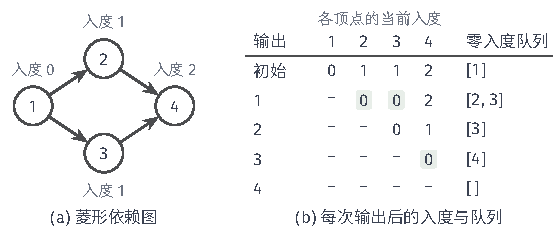
\includegraphics[width=94.8mm]{figures/01-basic-mathematics/04-graphs/tikz/c2-kahn-diamond/figure.pdf}
  \caption{Kahn算法在菱形依赖图上的执行。(a)依赖图及各顶点的初始入度。(b)每输出一个顶点后各顶点的当前入度（“--”表示已输出）与零入度队列；绿色底纹标出刚降为$0$、随即入队的入度。顶点$4$要等两个前驱都输出后才入队。}
  \label{fig:graph-trav-kahn}
\end{figure}

输出$1$之后，$2$和$3$同时位于队列中，这表示两项任务可以同时执行，或以任意先后执行。若先取$3$，就得到同样合法的$1,3,2,4$。队列中同时有多个零入度顶点时选哪一个，决定了得到哪个拓扑序。

\paragraph{计算开销}
统计入度要扫描每条弧一次；之后每个顶点入队、出队各一次，每条弧在其起点输出时被扣减一次。总时间为$O(n+m)$，入度数组、队列与输出序列占$O(n)$额外空间。若要求结果可复现，例如在多个零入度顶点中总是选编号最小的，就要把普通队列换成优先队列，每次入队、出队需要$O(\log n)$时间，总时间变为$O(m+n\log n)$。

\subsection{基于DFS的拓扑排序}
\label{sec:graph-trav-dfs-toposort}

\paragraph{逆完成次序}
第~\ref{sec:graph-trav-dfs-orders}节已经在一个例子中看到，把深度优先遍历的完成次序反转，弧的起点就排在了终点前面。下面说明这在无环图中总是成立。

\begin{theorem}[逆完成次序是拓扑序]
\label{thm:graph-trav-dfs-toposort}
对有向无环图执行一次覆盖全部顶点的深度优先遍历，则对每条弧$u\to v$都有$f(v)<f(u)$。因此按完成时刻从大到小排列顶点，得到一个拓扑序。
\end{theorem}

\begin{proof}
考察$u$检查弧$u\to v$的时刻，此时$u$处于处理中，按$v$的状态分三种情况。若$v$未发现，它将以$u$为父指针被发现，由引理~\ref{lem:graph-trav-dfs-nesting}，$f(v)<f(u)$。若$v$已完成，$f(v)$早于当前时刻，而$u$尚未完成，同样$f(v)<f(u)$。若$v$处于处理中，$u\to v$是一条回边，由定理~\ref{thm:graph-trav-directed-cycle}图中有有向环，与假设矛盾，这种情况不会发生。
\end{proof}

于是得到第二种构造：执行覆盖全部顶点的三色深度优先遍历；一旦遇到回边，就沿父指针返回一个有向环，拒绝输出排序；若始终没有回边，把完成次序反转后输出。实现时可以在每个顶点完成时把它放到输出序列的最前面，遍历结束时序列就已是逆完成次序。

\paragraph{与Kahn算法的结果比较}
在同一个菱形依赖图上，从$1$出发、按编号读取出邻居：发现$1,2,4$，$4$完成，$2$完成；回到$1$后发现$3$，$3$的出邻居$4$已完成，$3$完成；最后$1$完成。完成次序为$4,2,3,1$，反转得$1,3,2,4$，见图~\ref{fig:graph-trav-dfs-toposort}。它与Kahn算法给出的$1,2,3,4$不同，但两者都是合法拓扑序：把顶点按次序从左到右排开，四条弧全部指向右方。拓扑序可能不唯一，检验一个输出是否正确，标准是逐条弧核对先后，而不是与某一个特定答案比较。

\begin{figure}[!htb]
  \centering
  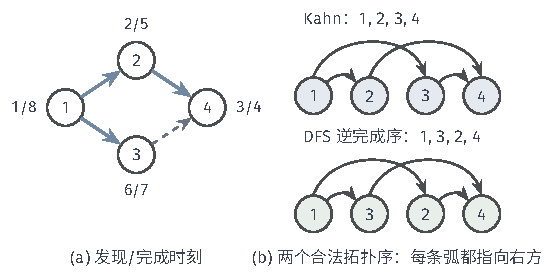
\includegraphics[width=93.8mm]{figures/01-basic-mathematics/04-graphs/tikz/c2-dfs-topological-order/figure.pdf}
  \caption{基于深度优先遍历的拓扑排序。(a)菱形依赖图上从$1$出发的深度优先遍历，旁注为发现/完成时刻，蓝色箭头为父指针对应的弧，虚线弧$3\to4$检查时$4$已完成。(b)Kahn算法得到的$1,2,3,4$与逆完成次序$1,3,2,4$，两种排列下每条弧都从左指向右，都是合法拓扑序。}
  \label{fig:graph-trav-dfs-toposort}
\end{figure}

\paragraph{必须覆盖全部顶点}
只从一个起点遍历时，得到的只是它可达部分的完成次序。在菱形图中若只从$2$出发，只能到达$2,4$，反转后是$2,4$，漏掉了$1$和$3$。也不能把各次重启的结果分别反转后简单拼接：先从$2$出发得到$2,4$，再从$1$出发得到$1,3$，拼成$2,4,1,3$，违反了弧$1\to2$。正确做法是把整次遍历的完成次序$4,2,3,1$作为一个整体反转，得到$1,3,2,4$；定理~\ref{thm:graph-trav-dfs-toposort}的证明对跨越不同起点的弧同样成立。

\paragraph{两种方法的选择}
两种方法的时间都是$O(n+m)$。Kahn算法显式地维护“当前可以执行的任务”这一集合，适合需要逐步列出可并行任务、或按某种优先规则选择任务的场合。基于深度优先遍历的方法不需要入度数组，在已经要做深度优先遍历、或需要在有环时给出环的场合可以直接复用同一次遍历。对一般有向图，可以先用第~\ref{sec:graph-trav-scc}节的方法求出强连通分量并缩点，再对无环的缩点图做拓扑排序。第~\ref{sec:graph-shortest-paths}节在有向无环图上计算最短路时，就是按拓扑序逐个处理顶点。

\section{基于分隔集的分块}
\label{sec:graph-separator-blocks}

大图上的计算常常希望“分而治之”：把图拆成几块分别处理，再在块与块的连接处汇总。第~\ref{sec:graph-connectivity-separation}节定义了分隔集：删除一个顶点集$S$后，若某些顶点之间不再有路径，$S$就把它们分隔开。本节接受一个给定的候选集$S$，用连通分量计算检验它是否真的把图拆成了几侧，再把$S$加回各侧，得到共享接口的局部块。本节只负责结构上的分块：怎样找到好的分隔集不在这里讨论，块上的数值怎样沿接口组合则放在第~\ref{chap:graph-dynamic-programming}章。

\subsection{删除集合后的分量}
\label{sec:graph-trav-delete-separator}

\paragraph{输入、输出与三种结果}
输入是无向图$\mathcal G=(V,E)$和一个候选集合$S\subseteq V$。删除$S$中的顶点及与它们关联的边，得到$\mathcal G-S$，即$V\setminus S$上的诱导子图；对它计算连通分量$C_1,\ldots,C_r$。不同的$C_j$之间在$\mathcal G-S$中没有边，所以原图中从$C_j$到$C_k$（$j\neq k$）的任何路径都必须经过$S$。按$r$的取值有三种结果：$r\geq2$时，$S$把图拆成了$r$侧，任取两个不同分量中的顶点，$S$都把它们分隔开；$r=1$时，删除$S$后其余顶点仍然连通，$S$没有形成多侧拆分；$r=0$时$S=V$，余图为空，也谈不上拆分。是否拆分成功只能由计算结果判断，不能因为输入被称作“分隔集”就默认成立。

\begin{algorithm}[删除候选集后的分量]
\label{alg:graph-trav-separator-components}
输入：无向图的邻接表，候选集合$S\subseteq V$。输出：$\mathcal G-S$的连通分量$C_1,\ldots,C_r$，以及拆分是否成功（$r\geq2$）。
\begin{enumerate}
  \item 用一个布尔数组标记$S$中的顶点为“屏蔽”，不修改原邻接表。
  \item 对未屏蔽的顶点执行算法~\ref{alg:graph-trav-components}：外层扫描跳过屏蔽顶点，遍历时读到屏蔽的邻居一律跳过。
  \item 输出各分量；若$r\geq2$报告拆分成功，$r=1$报告未拆分，$r=0$报告余图为空。
\end{enumerate}
\end{algorithm}

\paragraph{贯穿图上的检验}
在贯穿四点图上取$S=\{2,3\}$。删除$2,3$后，与它们关联的边$\{1,2\}$、$\{1,3\}$、$\{2,3\}$、$\{2,4\}$、$\{3,4\}$全部消失，只剩顶点$1$和$4$，而$\{1,4\}$不是原图的边，所以余图有两个分量$\{1\}$与$\{4\}$，见图~\ref{fig:graph-trav-separator-blocks}(a)。$S=\{2,3\}$成功地分隔了$1$和$4$。作为对照，取$S=\{1\}$，删除后剩下的$2,3,4$两两相邻，构成一个三角形，余图只有一个分量，见图~\ref{fig:graph-trav-separator-blocks}(c)，$\{1\}$不是有效的拆分。贯穿图中删去任何单个顶点都不会断开余图：删去$1$或$4$剩下三角形，删去$2$或$3$剩下一条路径，所以它没有割点，至少要删两个顶点才能拆开。

\paragraph{检验与优化是两个问题}
上面的计算回答的是“这个给定的$S$是否拆开了图”，用$O(n+m)$时间就能完成。它不回答“最小的拆分集合是什么”。若想通过检验来找最小的分隔集，就要逐个尝试候选集合：大小为$k$的候选集有$\binom{n}{k}$个，每个都要做一次连通分量计算，规模稍大就无法承受。寻找小的分隔集需要另外的方法，它们不是一次连通标记能自动给出的。

\subsection{局部块与公共接口}
\label{sec:graph-trav-blocks-interfaces}

\paragraph{把接口加回各侧}
删除$S$之后，各分量之间不再相连；但原图中分量内的顶点与$S$之间的边、$S$内部的边也随之丢失了。要把原图完整地分成几块，需要把$S$加回每一侧，得到\term{局部块}（local block）
\[
\mathcal B_j=\mathcal G[C_j\cup S],\qquad j=1,\ldots,r,
\]
其中$S$称为各块的公共接口。图~\ref{fig:graph-trav-separator-blocks}(b)中两个局部块是$\mathcal G[\{1,2,3\}]$与$\mathcal G[\{2,3,4\}]$，都是三角形，共享顶点$2,3$和边$\{2,3\}$。

\begin{figure}[!htb]
  \centering
  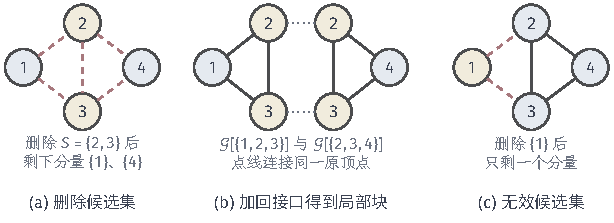
\includegraphics[width=103.9mm]{figures/01-basic-mathematics/04-graphs/tikz/c2-separator-blocks/figure.pdf}
  \caption{基于分隔集的分块。黄色顶点为候选删除集，红色虚线为随之删去的边。(a)贯穿四点图删除$S=\{2,3\}$后剩下两个分量$\{1\}$与$\{4\}$；(b)把$S$加回各侧得到两个局部块，两块中的$2,3$是同一批原顶点（点线相连），边$\{2,3\}$被两块共同引用；(c)删除$\{1\}$后余下三角形仍然连通，没有形成拆分。}
  \label{fig:graph-trav-separator-blocks}
\end{figure}

局部块覆盖了原图的每一条边。原图的一条边有三种可能：两端都在某个$C_j$中，或一端在$C_j$、一端在$S$中，这两种边都属于$\mathcal B_j$；两端都在$S$中，这样的边属于每一个块。由于不同分量之间没有边，不存在第四种情况。因此，原图的全部信息都保存在这些块中，块与块之间只通过$S$发生联系。

\paragraph{共享引用与复制}
不同局部块中的接口顶点是同一批原顶点，而不是可以各自独立变化的副本。若以后要给顶点赋值，同一个接口顶点在各块中必须取相同的值；若块中记录了边的数据，$S$内部的边被多个块同时看到，汇总时不能重复计数。因此表示局部块时，应保存接口顶点和接口边的唯一身份，各块只引用它们，而不是把原图的一部分真正复制几份后各自修改。

\paragraph{计算与存储开销}
屏蔽$S$并计算余图分量需要$O(n+m)$时间。输出局部块的存储另计：各块顶点数之和为$\sum_j(|C_j|+|S|)=(n-|S|)+r|S|$，接口顶点被重复列出$r$次；$S$内部的边也在每个块中出现一次。$r$和$|S|$都较小时，这部分额外存储可以忽略；接口很大或块很多时，就应采用共享引用。

\paragraph{小接口不保证块内简单}
接口小，只说明块与块之间的联系少，并不说明每个块内部简单。例如两个各有$100$个顶点的完全图只共用一个顶点，删除这个顶点就把图拆成两侧，接口大小为$1$，可每个局部块仍是一个$100$个顶点的完全图。分块的收益取决于后续计算在块内需要做什么。第~\ref{chap:graph-dynamic-programming}章会看到，当计算由许多只涉及少数顶点的局部项组成时，固定接口上的取值后各块可以分别处理，这时接口大小直接决定中间表的规模；那里还会把一次分块推广为多层的树分解。

\section{顶点标记与结构比较}
\label{sec:graph-wl-refinement}

第~\ref{sec:graph-isomorphism}节把两个图同构定义为存在保持邻接的顶点双射，并指出顶点数、边数、度分布等必要条件一般不足以判定同构。直接尝试所有$n!$个双射又不可行。本节介绍一种折中的办法：给每个顶点一个标记，然后反复根据“自己是什么、邻居都是什么”更新标记，使结构上不同的顶点逐渐得到不同的标记。这些标记不依赖顶点的编号，可以用来比较两个图；但我们也会看到，它并不能区分所有不同构的图。

\subsection{邻域标记与多重集合}
\label{sec:graph-trav-neighborhood-labels}

\paragraph{从度数到邻居的类别}
无属性的图里，顶点一开始没有任何可区分的信息，可以给所有顶点同一个初始标记；带属性的图则可以把属性作为初始标记。记顶点$i$的初始标记为$c_i^{(0)}$。第一步自然的细化是看邻居个数，即度数：三点路径$1\text{--}2\text{--}3$中，两个端点各有一个邻居，中点有两个邻居，于是端点与中点被区分开。更进一步，不只数邻居有几个，还要看邻居分别属于哪一类、每类有几个。这样，“有两个端点邻居的顶点”和“有一个端点邻居、一个中点邻居的顶点”也能被区分。

\paragraph{多重集合}
怎样记录“邻居都属于哪些类、各几个”？普通集合不行：两个邻居都是$A$类时，集合$\{A,A\}$就是$\{A\}$，丢失了次数。按顶点编号排出邻居标记的序列也不行：同一个顶点的邻居换一种编号，序列的次序就变了，而我们要的信息不应依赖编号。合适的对象是\term{多重集合}（multiset）：它像集合一样不计次序，又像序列一样记录每个元素出现的次数。用双花括号表示多重集合，例如$\{\!\{A,A,B\}\!\}$含两个$A$、一个$B$，它不等于$\{\!\{A,B\}\!\}$，但等于$\{\!\{A,B,A\}\!\}$。实际比较两个多重集合时，可以先把元素排序，再逐项比较。

\paragraph{签名与统一编码}
把顶点自己的旧标记与邻居标记的多重集合放在一起，称为该顶点在第$t$轮的签名：
\[
\sigma_i^{(t)}=\Bigl(c_i^{(t)},\ \{\!\{c_j^{(t)}:j\in N(i)\}\!\}\Bigr).
\]
签名完全由图的结构和当前标记决定，与顶点编号无关。比较两个图时，两图必须使用同一种初始标记规则，并且把签名翻译成新标记时使用同一本“字典”：同一个签名在两个图中必须得到同一个新标记。否则即使两图结构相同，标记的名称也可能对不上。

还要注意，不能为了“容易区分”而给每个顶点附上唯一的编号作为初始标记。那样所有顶点一开始就互不相同，比较的就不再是无属性图的结构，而是“编号也必须对应”的另一个问题。只有当属性本身是图的数据、并随顶点重编号一起移动时，才把它作为初始标记，这时比较的是带属性的图。

\subsection{1-WL标记细化}
\label{sec:graph-trav-wl-algorithm}

\paragraph{同步细化的规则}
有了签名，更新规则就是：所有顶点同时计算签名，签名相同的顶点得到相同的新标记，签名不同的得到不同的新标记。

\begin{definition}[1-WL标记细化]
\label{def:graph-trav-wl-refinement}
给定无向图$\mathcal G=(V,E)$与初始标记$c_i^{(0)}$，对$t=0,1,2,\ldots$同步计算
\begin{equation}
c_i^{(t+1)}=\operatorname{enc}\bigl(\sigma_i^{(t)}\bigr)
=\operatorname{enc}\Bigl(c_i^{(t)},\ \{\!\{c_j^{(t)}:j\in N(i)\}\!\}\Bigr),
\qquad i\in V,
\label{eq:graph-trav-wl-update}
\end{equation}
其中$\operatorname{enc}$是单射，即不同的签名映为不同的新标记。这一过程称为一维Weisfeiler--Leman标记细化（1-WL），也称\term{颜色细化}（color refinement）。第$t$轮的标记把$V$划分为若干类，记为$\mathcal P^{(t)}$。
\end{definition}

“同步”是指第$t+1$轮的所有签名都只读取第$t$轮的标记：先为全部顶点算完签名，再统一替换。若边算边替换，后处理的顶点会读到一部分新标记、一部分旧标记，结果就依赖处理次序，从而依赖编号。$\operatorname{enc}$的单射要求是数学上的约定；实际程序常用哈希函数把签名压缩成整数，而不同签名可能碰巧得到相同的哈希值。所以实现时应当比较完整的签名，或用字典给每个新出现的签名分配一个新整数，不能只凭哈希值判定两个签名相等。

\paragraph{三点路径上的细化}
图~\ref{fig:graph-trav-wl-path}从三点路径$1\text{--}2\text{--}3$开始，初始标记全为$A$。第$0$轮的签名为：端点$1,3$是$(A,\{\!\{A\}\!\})$，中点$2$是$(A,\{\!\{A,A\}\!\})$。两种签名不同，分别编码为$B$与$C$，得到$c^{(1)}=(B,C,B)$，划分为$\{1,3\}$、$\{2\}$。第$1$轮的签名为：端点是$(B,\{\!\{C\}\!\})$，中点是$(C,\{\!\{B,B\}\!\})$，编码为$D$与$E$，得到$c^{(2)}=(D,E,D)$。标记的名称换了，但划分仍是$\{1,3\}$、$\{2\}$，与上一轮相同，细化到此停止。

\begin{figure}[!htb]
  \centering
  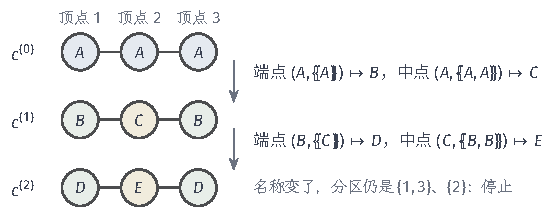
\includegraphics[width=94.0mm]{figures/01-basic-mathematics/04-graphs/tikz/c2-wl-path-refinement/figure.pdf}
  \caption{三点路径上的1-WL标记细化。每行是一轮标记，颜色表示所属的类；右侧是由签名得到新标记的编码。第一轮把端点与中点分开；第二轮标记名称改变，但划分仍为$\{1,3\}$、$\{2\}$，细化停止。}
  \label{fig:graph-trav-wl-path}
\end{figure}

\paragraph{只拆分不合并，有限轮后停止}
上例显示，判断停止要看划分，而不是看标记的名称。下面的引理说明划分只会越来越细，并且一旦某轮没有变化，以后也不会再变。

\begin{lemma}[1-WL的单调性与停止]
\label{lem:graph-trav-wl-refine}
对定义~\ref{def:graph-trav-wl-refinement}中的划分：（1）$\mathcal P^{(t+1)}$是$\mathcal P^{(t)}$的细分，即第$t+1$轮同类的顶点在第$t$轮也同类；（2）若$\mathcal P^{(t+1)}=\mathcal P^{(t)}$，则以后各轮划分都不再改变；（3）至多$n-1$轮严格细分后，划分就停止变化。
\end{lemma}

\begin{proof}
（1）若$c_i^{(t+1)}=c_j^{(t+1)}$，由$\operatorname{enc}$是单射得$\sigma_i^{(t)}=\sigma_j^{(t)}$，签名的第一个分量相等，即$c_i^{(t)}=c_j^{(t)}$。

（2）两轮划分相同，意味着存在标记之间的一一对应$\varphi$，使得对每个顶点$c_i^{(t+1)}=\varphi(c_i^{(t)})$。把$\varphi$作用到签名的每个分量上，得到$\sigma_i^{(t+1)}=\bigl(\varphi(c_i^{(t)}),\{\!\{\varphi(c_j^{(t)}):j\in N(i)\}\!\}\bigr)$。$\varphi$是一一对应，所以$\sigma_i^{(t+1)}=\sigma_k^{(t+1)}$当且仅当$\sigma_i^{(t)}=\sigma_k^{(t)}$，即$c_i^{(t+2)}=c_k^{(t+2)}$当且仅当$c_i^{(t+1)}=c_k^{(t+1)}$。因此$\mathcal P^{(t+2)}=\mathcal P^{(t+1)}$，依此类推。

（3）每次严格细分至少使类的个数加一，类的个数从至少$1$开始、不超过$n$，所以严格细分至多$n-1$次。由（2），第一次没有变化之后就再也不会变化。
\end{proof}

\paragraph{计算开销}
每一轮要为每个顶点读取全部邻居的标记，共$O(n+m)$次读取；把顶点$i$的邻居标记排序成多重集合的规范形式需要$O(d_i\log d_i)$时间；再把全部签名排序或查字典以分配新标记。一轮的总代价为$O((n+m)\log n)$量级。由引理~\ref{lem:graph-trav-wl-refine}，至多$n$轮就能确认划分稳定（最后一轮用于确认没有变化），所以总时间不超过$O(n(n+m)\log n)$。实际图上细化往往在少数几轮内稳定，总开销远小于这个上界。

\subsection{判别能力与局限}
\label{sec:graph-trav-wl-power}

\paragraph{在不交并上比较两个图}
要用1-WL比较图$\mathcal G_1$与$\mathcal G_2$，把两图放在一起看成一个不交并，用同一个初始标记规则和同一本字典同步细化，然后在每一轮分别统计两图中每种标记出现的次数。这种比较方法称为\term{一维Weisfeiler--Leman检验}（1-dimensional Weisfeiler--Leman test）。若某一轮两图的计数不同，就可以断定两图不同构；若计数在细化稳定前始终相同，只能说这一方法没有区分它们。

为什么计数不同就能断定不同构？设$\pi$是从$\mathcal G_1$到$\mathcal G_2$的同构，且初始标记满足$c_{\pi(i)}^{(0)}=c_i^{(0)}$（无属性时所有初始标记相同，自然满足；有属性时同构本来就要求保持属性）。$\pi$把$i$的邻居一一映为$\pi(i)$的邻居，对轮数归纳可得$\sigma_{\pi(i)}^{(t)}=\sigma_i^{(t)}$，于是$c_{\pi(i)}^{(t+1)}=c_i^{(t+1)}$。$\pi$是顶点之间的双射，每种标记在两图中的出现次数就相同。同样的推理说明，对同一个图重新编号顶点（用第~\ref{sec:graph-isomorphism}节的置换表示），各顶点的标记随之移动，标记计数不变：1-WL的结果不依赖编号，也不依赖图的画法。

例如，四个顶点的路径与四个顶点的星形都有$4$个顶点、$3$条边。初始标记全为$A$时，第一轮路径得到两个“一个邻居”的端点和两个“两个邻居”的内点，星形得到三个“一个邻居”的叶和一个“三个邻居”的中心，计数不同，两图不同构。这一轮区分的其实就是度分布，更多轮次则会区分邻居的度、邻居的邻居的度，等等。

\paragraph{六环与两个三角形}
1-WL的判别能力是有限的。图~\ref{fig:graph-trav-wl-limitation}中，六个顶点的环与两个不相连的三角形都有$6$个顶点、$6$条边，每个顶点的度都是$2$。初始标记全为$A$时，每个顶点的签名都是$(A,\{\!\{A,A\}\!\})$，所有顶点得到同一个新标记；下一轮又是同样的情形。标记从第一轮起就稳定为一类，两图的计数始终相同，1-WL无法区分它们。可是它们并不同构：六环是连通的，而两个三角形构成两个连通分量。用第~\ref{sec:graph-trav-components-forest}节的方法数一下连通分量，就能立刻把它们分开。

\begin{figure}[!htb]
  \centering
  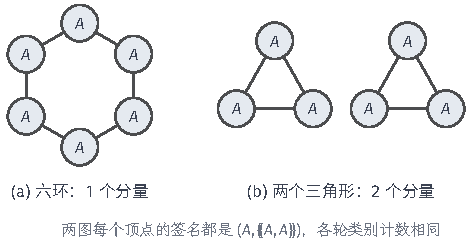
\includegraphics[width=79.5mm]{figures/01-basic-mathematics/04-graphs/tikz/c2-wl-cycle-triangles/figure.pdf}
  \caption{1-WL的局限。(a)六顶点环与(b)两个不相连的三角形初始标记全为$A$；每个顶点在每一轮都看到两个同类邻居，签名恒为$(A,\{\!\{A,A\}\!\})$，两图各轮的标记计数完全相同。两图分量数不同，并不同构。}
  \label{fig:graph-trav-wl-limitation}
\end{figure}

这个例子说明了1-WL的本质：每个顶点只能看到以自己为中心、逐轮向外扩大的邻域中“各类邻居有几个”，而六环和三角形上的每个顶点，无论看多少轮，看到的局部情形都一样。连通分量数这种整体性质，局部的计数无法反映。因此1-WL计数不同可以作为不同构的证据，计数相同则不能作为同构的证明。实践中常把它与分量数、环长等其他检验结合使用，各种检验互为补充；要确认同构，仍需给出一个实际的保持邻接的双射并逐边核对。

\section{本章小结}
\label{sec:graph-traversal-summary}

本章的出发点是：第~\ref{chap:graph-objects}章定义的可达、分量、无环和同构，怎样在一张实际的图上算出来。回答的共同方式是沿邻接表有组织地访问顶点，用少量状态记住已经知道的东西，而不去枚举路径或双射。表~\ref{tab:graph-trav-summary}对照了本章各方法所维护的状态、输出和计算时间。

\begin{table*}[!htb]
  \centering
  \caption{本章方法维护的状态、输出与时间。时间均以邻接表存储计，$n$为顶点数，$m$为边数或弧数。}
  \label{tab:graph-trav-summary}
  \small
  \begin{tabular}{@{}llll@{}}
    \toprule
    方法 & 维护的状态 & 输出 & 时间 \\
    \midrule
    广度优先遍历 & 队列、距离、父指针 & 最少边数与一条最短路线 & $O(n+m)$ \\
    深度优先遍历 & 三色状态、栈帧、时刻 & 发现次序、完成次序、回边 & $O(n+m)$ \\
    分量编号 & 外层扫描、分量号 & 连通分量、生成森林 & $O(n+m)$ \\
    并查集 & 父指针树、集合大小 & 加边过程中的分量代表 & 每次$O(\log n)$ \\
    Kosaraju算法 & 完成次序、反向图 & 强连通分量、缩点图 & $O(n+m)$ \\
    Kahn算法 & 当前入度、零入度队列 & 拓扑序或有环报告 & $O(n+m)$ \\
    分隔集分块 & 屏蔽标记、分量号 & 余图分量、局部块 & $O(n+m)$ \\
    1-WL细化 & 各轮标记、签名字典 & 稳定划分、标记计数 & 每轮$O((n+m)\log n)$ \\
    \bottomrule
  \end{tabular}
\end{table*}

这些输出回答的是不同的问题。广度优先遍历的层数回答“离起点最少几步”，深度优先遍历的完成次序回答“谁的后续全部探完”，它在无环图上给出拓扑序，在一般有向图上把强连通分量按缩点图的先后分离出来。并查集的代表元回答“在已加入的边下是否连通”，1-WL的标记回答“局部邻域在计数意义下是否一样”。同一张图上，这些量可以同时计算，但不能互相替代：深度优先的父路径不是最短路线，发现次序不是拓扑序，并查集的父指针不是原图的边，1-WL计数相同也不是同构的证明。

判断一个算法的输出是否正确，标准是看它是否满足相应的结构条件，而不只是看算法是否停止。广度优先遍历的父路径应恰有$d(v)$条边；生成森林应有$n-c$条边且无环；拓扑序应使每条弧从前指向后；有环报告应附带一个可以逐弧核对的环；强连通分量在第二遍中不应越过已标记的分量；分块检验应报告余图实际有几个分量。各节的定理正是把这些条件与算法的状态联系起来的依据。

本章得到的可达区域、生成森林和依赖次序，都只描述了“能否连接、按什么次序”，没有比较不同路线或不同边集的代价：广度优先遍历只数边数，生成森林只保证连通。下一章在这些可行结构的基础上引入边上的数值，研究最短路、最小生成树、最大流、最小费用流和匹配；本章的并查集用于Kruskal算法，拓扑序用于有向无环图上的最短路递推。第~\ref{chap:graph-dynamic-programming}章则沿着第~\ref{sec:graph-separator-blocks}节的接口思想，把局部块上的计算组织起来。


\chapter{图上的组合优化}
\label{chap:graph-optimization}

前两章研究图上“有什么连接”和“怎样把连接找出来”：第~\ref{chap:graph-objects}章定义路径、树与分隔，第~\ref{chap:graph-traversal}章用遍历恢复路径、提取连通结构、排出依赖次序。那里的问题大多只问存在与否，一条路线或一棵生成树只要满足结构要求就算完成。本章给边配上数值，并在满足结构要求的众多候选中挑出数值最好的一个。在同一张交通网络上，可以选一条总长度最短的路线，可以铺一组总造价最低、又能连通所有站点的线路，也可以在每条道路的通行上限内安排尽可能多的输送量。三个问题的选择对象分别是一条路径、一组边和每条弧上的一个数，边旁的数字分别表示长度、造价和容量。因此，每个问题都要先固定选择对象与目标，再讨论算法。

本章依次处理六个问题。第~\ref{sec:graph-shortest-paths}节在有向图上寻找起点到各顶点的最短路。三种算法共用“距离标签”和“松弛”两个操作：有向无环图按拓扑序一遍完成；Bellman--Ford算法允许标签反复修正，并能识别负环的影响；Dijkstra算法在边长非负时每次永久确定一个顶点。第~\ref{sec:graph-minimum-spanning-tree}节在无向图上选总权最小的生成树，Kruskal算法与Prim算法都依靠同一条割性质，用交换论证说明每次选边是安全的。第~\ref{sec:graph-max-flow}节在容量限制下最大化源到汇的输送量，引入可以撤回旧流量的残量网络。它证明一个可行流最优当且仅当残量网络中没有增广路径，并由按最少弧数选路的Edmonds--Karp算法得到“最大流值等于最小割容量”。

后三节在最大流的基础上改变目标或结构。第~\ref{sec:graph-min-cost-flow}节固定各点的供需量，转而最小化输送费用。最优性改由残量网络中没有负费用环来刻画，网络单纯形法把可行流组织成生成树，沿树上的基本环逐步降低费用。第~\ref{sec:graph-matching}节在二部图中选取互不共享端点的边，交替路径扮演增广路径的角色，单位容量的流网络把匹配和最大流联系起来。第~\ref{sec:graph-assignment}节要求每个对象都完成配对并最小化总成本，匈牙利算法同时维护给出成本下界的顶点标号与由紧边组成的匹配，两者相遇时即得最优解。

六个问题的算法各不相同，论证却有共同的样式：先指出算法维护什么状态，再说明哪一条递推、交换或上下界论证排除了更好的候选，最后交代计算开销与条件失效时会发生什么。许多算法除了给出答案，还附带一份可以独立复核的“证书”，如最短路的逐弧不等式、同值的流与割、同值的指派与标号。第~\ref{sec:graph-optimization-summary}节把这些证书与各自的成立条件并列比较。全章记顶点数为$n=|V|$，无向边数为$m$，有向弧数为$a$。除非另有说明，图以邻接表存储，边长、容量、成本等数值另存在与边对应的数组中。

% 第3章第1节：最短路（路径成本与三类距离结果、距离标签与松弛、DAG递推、Bellman--Ford、Dijkstra、方法比较与结果检验）。

\section{最短路}
\label{sec:graph-shortest-paths}

第~\ref{sec:graph-bfs}节的广度优先遍历给出从起点出发的最少边数。可是在道路网络中，每段路的长度不同；在任务调度中，从一个状态转到另一个状态的代价也各不相同。这时要比较的是路线上各段数值之和，经过的边数少不等于总成本低。

本节在有向加权图上研究这个问题。先说明路线成本怎样定义、距离可能出现哪几类结果，再建立三种算法共用的距离标签与松弛操作。随后依次介绍三种算法：有向无环图上的递推利用无环次序，Bellman--Ford算法允许标签反复修正，Dijkstra算法在边长非负时永久确定标签。每种算法的正确性论证紧接在各自的机制之后，最后比较三者的适用范围，并说明怎样检验一份最短路结果。

\subsection{路径成本与最短路问题}
\label{sec:graph-opt-path-cost}

设$\mathcal G=(V,E)$是有限有向图，每条弧$u\to v$带有一个实数\emph{长度}$\ell_{u,v}$。长度可以表示距离、时间或转换代价，也允许为负，例如某次转换带来收益。对一条行走$W=(v_0,v_1,\ldots,v_k)$，规定它的成本为沿途弧长之和：
\[
  \ell(W)=\sum_{r=1}^{k}\ell_{v_{r-1},v_r}.
\]
只含一个顶点的零步行走成本为零。所有长度都等于$1$时，成本就是边数，回到广度优先遍历的情形；一般长度下两者不再一致。例如$s$到$t$有一条长$5$的直达弧，又有经过$u$、两段各长$1$的路线，两步路线反而更短。

\paragraph{两种候选集合}
寻找“最短路线”时，必须先说清候选集合是什么。一种选择只允许简单路径，即不重复经过顶点的路径；另一种允许一般的行走，顶点和弧都可以重复。有限图中简单路径只有有限条，因此只要终点可达，最小值一定存在；行走可以无限地绕圈，候选有无穷多个，只能谈成本的下确界。

\begin{definition}[最短路问题]
\label{def:graph-opt-shortest-path}
给定有限有向图$\mathcal G=(V,E)$、弧长$\ell_{u,v}\in\mathbb R$与源点$s\in V$。对每个顶点$v$，记$\mathcal W_{s,v}$为从$s$到$v$的全部有限行走组成的集合，称
\[
  \delta(v)=\inf_{W\in\mathcal W_{s,v}}\ell(W)
\]
为$s$到$v$的\term{最短路}距离，约定空集的下确界为$+\infty$。若某条行走$W\in\mathcal W_{s,v}$满足$\ell(W)=\delta(v)$，就称$W$是一条$s$到$v$的最短路。求出全部$\delta(v)$及相应路线的问题称为单源最短路问题。
\end{definition}

本节的算法计算的都是行走下确界$\delta(v)$。在多数情形中它与简单路径的最小值一致，原因是行走中的绕圈部分可以删掉。设行走$W$两次经过顶点$x$，两次之间的一段是从$x$回到$x$的闭行走$C$，删去$C$得到更短的行走$W'$，并且$\ell(W')=\ell(W)-\ell(C)$。只要$C$的成本非负，删去它就不会增加成本。反复删除，直到不再有重复顶点，便得到一条成本不超过$\ell(W)$的简单路径。

\paragraph{负环与三类结果}
删除闭合段的论证只在闭行走成本非负时有效。成本为负的有向环称为\term{负环}（negative cycle）。若能从$s$走到某个负环，绕若干圈后再走到$v$，则每多绕一圈，成本就再降低一次，于是$\delta(v)=-\infty$。这并不表示存在一条“长度为负无穷的路径”，而是说任何有限成本都能被另一条行走打破。反过来，若没有这样“从$s$可达、又能到达$v$”的负环，那么$s$到$v$的行走中出现的任一闭合段也不可能为负。原因是一条成本为负的闭行走，在第一个重复顶点处切开，总能分出一个简单环，剩下的部分仍是闭行走；重复这一切分，闭行走的成本就写成若干个简单环的成本之和，其中必有一个为负，而这个环同样从$s$可达、又能到达$v$。因此在这种情形下，所有闭合段都可以删除，$\delta(v)$等于简单路径的最小成本，并且由一条简单路径达到。

综上，一次单源查询中，每个顶点的距离属于三类之一：不可达时$\delta(v)=+\infty$；可达且不受负环影响时$\delta(v)$为有限值，并由一条简单路径达到；能从某个$s$可达的负环到达时$\delta(v)=-\infty$。三类顶点可以出现在同一张图中。图~\ref{fig:graph-opt-distance-outcomes}中，负环$a\to b\to a$只影响它自己及其后继$t$；旁支$u$不能从这个负环到达，距离仍是有限的$4$；另一个负环$x\to y\to x$从$s$出发到不了，对本次查询没有任何影响。所以不能因为图中某处有负环，就把全部顶点都标成负无穷。

\begin{figure}[!htb]
  \centering
  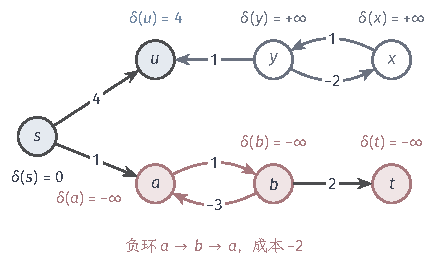
\includegraphics[width=73.801mm]{figures/01-basic-mathematics/04-graphs/tikz/c3-distance-outcomes/figure.pdf}
  \caption{单源最短路的三类结果同处一图（源点为$s$，弧旁数字为长度）。$a\to b\to a$的成本为$1-3=-2$，是从$s$可达的负环，环上的$a,b$及其后继$t$的距离为$-\infty$（红色）；旁支$u$不能从该负环到达，距离为有限值$4$（蓝色）；负环$x\to y\to x$从$s$不可达，$x,y$的距离为$+\infty$（灰色），弧$y\to u$也不会改变$u$的距离。}
  \label{fig:graph-opt-distance-outcomes}
\end{figure}

无向图中的负边需要特别注意。把无向边$\{u,v\}$换成两条同长的反向弧$u\to v$与$v\to u$以后，一条长为负的无向边自己就构成负环：沿它走过去再走回来，成本是两倍的负长度。因此，含负边的无向图不能直接套用本节的有向算法；本节默认讨论有向图，无向边只在长度非负时换成一对反向弧。

\subsection{距离标签与松弛}
\label{sec:graph-opt-relaxation}

三种算法都不直接枚举行走，而是为每个顶点保存一个当前已知的最好成本，在发现更好的路线时更新它。设想已经知道一条从$s$到$u$、成本为$d(u)$的路线，又有弧$u\to v$，那么把这条弧接在路线末尾，就得到一条到$v$、成本为$d(u)+\ell_{u,v}$的路线。如果它比$v$目前记录的成本更低，就应该改用它。

\paragraph{标签与松弛操作}
为每个顶点$v$保存一个\term{距离标签}（distance label）$d(v)\in\mathbb R\cup\{+\infty\}$和一个前驱$p(v)$。初始时令$d(s)=0$，其余顶点$d(v)=+\infty$，前驱为空。对一条弧$u\to v$执行\term{松弛}（relaxation），是指比较当前标签$d(v)$与候选值$d(u)+\ell_{u,v}$：若$d(u)<+\infty$且
\[
  d(u)+\ell_{u,v}<d(v),
\]
就令$d(v)\leftarrow d(u)+\ell_{u,v}$、$p(v)\leftarrow u$；否则什么也不做。只有严格改善时才更新，因而标签只会下降，不会上升。

松弛只从有限标签出发延长路线，由此得到所有算法共用的一个不变量：\emph{每个有限标签$d(v)$都等于某条从$s$到$v$的行走的成本}。初始时只有$d(s)=0$有限，对应零步行走。若松弛把$d(v)$改为$d(u)+\ell_{u,v}$，则把$u$的那条行走接上弧$u\to v$，就得到成本恰为新标签的行走。由此立即得到$d(v)\geq\delta(v)$：标签永远是真实距离的上界。后面每种算法要做的，都是说明在适当的条件下，这个上界最终会降到$\delta(v)$。

图~\ref{fig:graph-opt-relaxation}画出一次松弛。左图中$v$原来经由$w$得到标签$8$；检查弧$u\to v$时，候选值$3+2=5$更小，于是标签改为$5$，前驱同时改为$u$。右图中$v$的标签已是$4$，候选值$5$不能改善它，标签和前驱都保持不变。距离数组和前驱数组必须同步修改：如果只改距离而不改前驱，回溯得到的路线成本就不再等于标签。

\begin{figure}[!htb]
  \centering
  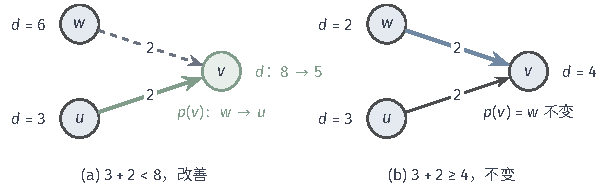
\includegraphics[width=102.993mm]{figures/01-basic-mathematics/04-graphs/tikz/c3-relaxation/figure.pdf}
  \caption{对弧$u\to v$松弛（顶点旁为当前标签，弧旁为长度）。(a) 候选值$d(u)+\ell_{u,v}=3+2=5$小于原标签$8$，标签改为$5$，前驱由$w$改为$u$（绿色表示被改善的标签与新的前驱弧，虚线为被替换的旧前驱弧）。(b) 原标签为$4$，候选值$5$不能改善，标签与前驱都不变。}
  \label{fig:graph-opt-relaxation}
\end{figure}

\paragraph{局部等式不能单独确定距离}
若没有可达负环，真实距离满足一组局部等式：$\delta(s)=0$，并且对每个可达的$v\neq s$，有$\delta(v)=\min_{u\to v}\{\delta(u)+\ell_{u,v}\}$。这只是说最短路的最后一条弧总来自某个前驱。但满足这组等式的数组不一定就是距离。设$s\to a$长$5$，$a\to b$与$b\to a$长都为$0$，则对任意$c\leq5$，取$D(s)=0$、$D(a)=D(b)=c$都满足
\[
  D(a)=\min\{D(s)+5,\ D(b)+0\}=c,\qquad D(b)=D(a)+0=c,
\]
而真实距离是$\delta(a)=\delta(b)=5$。这里的零成本环让$a,b$互相“支撑”着一个过低的值，却没有任何实际路线达到它。所以算法不能只去求解局部等式，而要从“源为零、其余为无穷”的初值出发，只沿实际路线下调标签，上面的不变量保证了这一点。初值保证标签不会无中生有，松弛保证每个标签都有路线见证，而松弛按什么次序进行、何时可以停止，则由各算法分别规定。

\paragraph{距离、前驱与访问状态}
算法通常维护三类数组，它们承担不同的职责。距离数组记录当前上界；前驱数组记录达到这个上界的最后一条弧，用于事后恢复路线；访问状态则记录算法自身的进度，例如Dijkstra算法中哪些顶点已经永久确定。前驱数组只在标签不再变化以后才能放心回溯。在一般有环图中，计算中途的前驱指针可能尚未形成从$s$出发的树；若存在可达负环，前驱指针甚至可能首尾相接成环。对于后面按轮次定义的递推，前驱还应与相应的轮次一同保存，才能把它们当作可回溯的路线。

\subsection{有向无环图上的最短路}
\label{sec:graph-opt-dag-shortest-path}

在一般的图中，一个顶点的标签可能在它的出弧已被松弛之后才下降，这时它的后继也必须随之更新。有向无环图没有这个问题：第~\ref{sec:graph-topological-order}节说明，有限有向无环图存在拓扑序，使每条弧的起点排在终点之前。按拓扑序处理顶点，轮到$v$时，所有指向$v$的弧都已被松弛，$v$的标签此后不会再变。

\begin{algorithm}[有向无环图上的最短路]
\label{alg:graph-opt-dag-shortest-path}
输入：有限有向无环图、弧长$\ell_{u,v}\in\mathbb R$、源点$s$。输出：全部距离$\delta(v)$与前驱$p(v)$。
\begin{enumerate}
  \item 求一个拓扑序$v_1,\ldots,v_n$；令$d(s)=0$，其余$d(v)=+\infty$，前驱为空。
  \item 按$i=1,\ldots,n$的顺序处理$v_i$：若$d(v_i)<+\infty$，对其每条出弧$v_i\to w$执行松弛。
  \item 对标签有限的顶点，沿前驱从终点退回$s$再反转，得到一条最短路；标签为$+\infty$的顶点报告不可达。
\end{enumerate}
\end{algorithm}

\paragraph{算例}
取弧$s\to a$长$2$、$s\to b$长$5$、$a\to b$长$-1$、$a\to t$长$5$、$b\to t$长$2$，它没有有向环，拓扑序可取$(s,a,b,t)$。处理$s$时，$a$的标签由$+\infty$改为$2$，$b$的标签由$+\infty$改为$5$。处理$a$时，候选$2+(-1)=1<5$使$b$改为$1$，同时$t$由$+\infty$改为$2+5=7$。处理$b$时，候选$1+2=3<7$使$t$改为$3$。最后处理$t$，它没有出弧。前驱为$p(a)=s$、$p(b)=a$、$p(t)=b$，从$t$回溯得到最短路$s\to a\to b\to t$，成本$2-1+2=3$。图~\ref{fig:graph-opt-dag-labels}记录了这个过程中各标签的变化。

\begin{figure}[!htb]
  \centering
  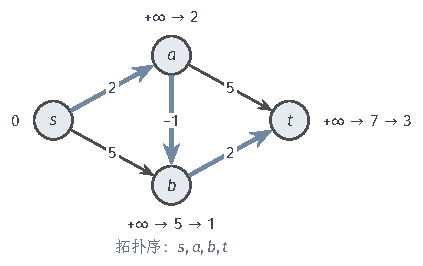
\includegraphics[width=71.635mm]{figures/01-basic-mathematics/04-graphs/tikz/c3-dag-labels/figure.pdf}
  \caption{按拓扑序$(s,a,b,t)$在有向无环图上松弛。顶点旁列出标签的变化次序，例如$b$先由处理$s$得到$5$，再由处理$a$改为$1$；蓝色粗弧是最终前驱弧，组成最短路$s\to a\to b\to t$（成本$3$）。负长度弧$a\to b$并不妨碍计算，因为正确性只依赖无环次序。}
  \label{fig:graph-opt-dag-labels}
\end{figure}

\paragraph{正确性}
上面的过程之所以能一遍完成，是因为处理到某个顶点时，所有可能到达它的路线都已考虑过。下面把这一点写成归纳证明。

\begin{theorem}[有向无环图上最短路的正确性]
\label{thm:graph-opt-dag-shortest-path}
设$\mathcal G$是有限有向无环图，弧长为任意实数。算法~\ref{alg:graph-opt-dag-shortest-path}结束时，对每个顶点$v$都有$d(v)=\delta(v)$；其中$\delta(v)=+\infty$当且仅当$v$从$s$不可达，其余$\delta(v)$均为有限值。
\end{theorem}

\begin{proof}
有向无环图中的行走不会重复顶点，因此每条行走都是简单路径，只有有限条，$\delta(v)$只可能是$+\infty$或有限值。松弛只改变弧终点的标签，而指向$v$的弧都从拓扑序中排在$v$之前的顶点出发，所以轮到$v$时它的标签已经不再改变。下面对拓扑序归纳，证明轮到$v$时$d(v)=\delta(v)$。

排在$s$之前的顶点从$s$不可达，它们的标签保持$+\infty$，与距离一致。对$v=s$，不存在回到$s$的非零步行走，故$\delta(s)=0=d(s)$。设$v$排在$s$之后，并且此前的顶点都已满足结论。若$v$不可达，则它的标签不可能变为有限值，因为有限标签总对应一条实际行走。若$v$可达，任取一条$s$到$v$的路径，设其最后一条弧为$u\to v$，则$u$排在$v$之前，路径前缀的成本不小于$\delta(u)$，归纳假设给出$\delta(u)=d(u)$。处理$u$时弧$u\to v$已被松弛，因而
\[
  d(v)\leq d(u)+\ell_{u,v}=\delta(u)+\ell_{u,v}\leq\text{该路径的成本}.
\]
路径是任取的，所以$d(v)\leq\delta(v)$。结合标签不变量$d(v)\geq\delta(v)$，得$d(v)=\delta(v)$。
\end{proof}

证明中只用到“前驱先于后继处理”，没有用到边长的符号，所以负长度弧不会造成任何问题。求拓扑序需要$O(n+a)$时间，之后每个顶点处理一次、每条弧松弛一次，总时间为$O(n+a)$，标签、前驱与拓扑序共占$O(n)$额外空间。

\paragraph{扩展示例：编辑距离}
许多递推问题的状态之间天然形成有向无环图，这时就是本小节的最短路问题。比较两段序列时，常问把序列$\bm a=(a_1,\ldots,a_p)$改写成$\bm b=(b_1,\ldots,b_q)$最少需要多少次单元素操作，允许的操作是插入一个元素、删除一个元素和把一个元素替换为另一个。以$(i,j)$表示“已把$\bm a$的前$i$个元素改写成$\bm b$的前$j$个元素”这一状态，最后一步只有三种可能：删去$a_i$，从$(i-1,j)$而来，成本为$1$；插入$b_j$，从$(i,j-1)$而来，成本为$1$；让$a_i$对应$b_j$，从$(i-1,j-1)$而来，相同时成本为$0$，不同时为一次替换，成本为$1$。于是最少操作数$E(i,j)$满足
\begin{equation}
  E(i,j)=\min\bigl\{E(i-1,j)+1,\ E(i,j-1)+1,\ E(i-1,j-1)+\mathbb I\{a_i\neq b_j\}\bigr\},
  \label{eq:graph-opt-edit-distance}
\end{equation}
边界为$E(i,0)=i$、$E(0,j)=j$，其中$\mathbb I\{\cdot\}$在条件成立时取$1$、否则取$0$。

每条状态弧都使$i+j$增加，所以状态图没有有向环，$E(p,q)$就是从$(0,0)$到$(p,q)$的最短路距离，称为两段序列的\term{编辑距离}（edit distance）。按$i+j$递增或逐行的顺序计算，正是在按拓扑序松弛。例如$\bm a=(A,B)$、$\bm b=(A,C,B)$时，三行表值依次为$(0,1,2,3)$、$(1,0,1,2)$、$(2,1,1,1)$，沿“匹配$A$、插入$C$、匹配$B$”得到距离$1$。全表连同前驱需要$O(pq)$时间与空间；只要距离值时保留相邻两行即可。更一般的序列对齐与动态时间规整留到信号与序列的应用部分，这里只说明它们的计算骨架是有向无环图上的最短路。

\subsection{Bellman--Ford算法}
\label{sec:graph-opt-bellman-ford}

图中有环时没有拓扑序可用：一个顶点的标签可能在它的出弧已被松弛之后才下降，一遍扫描不够。最直接的补救是反复扫描全部弧，直到标签不再变化。为了说清楚每一轮扫描得到了什么，先讲各轮彼此分开的同步版本。

\paragraph{同步递推}
令$d^{(0)}(s)=0$，其余$d^{(0)}(v)=+\infty$。第$k$轮只读取上一轮的标签，对每个顶点比较“沿用旧值”与“在上一轮的某条路线后再接一条弧”：
\begin{equation}
  d^{(k)}(v)=\min\Bigl\{d^{(k-1)}(v),\ \min_{u\to v}\bigl(d^{(k-1)}(u)+\ell_{u,v}\bigr)\Bigr\},\qquad k=1,2,\ldots,
  \label{eq:graph-opt-bellman-ford}
\end{equation}
没有入弧时内层最小值取$+\infty$。实现上，每轮先复制上一轮的标签数组，再逐弧用旧数组计算候选值、更新新数组。这样定义的标签有一个清楚的含义。

\begin{lemma}[同步标签的含义]
\label{lem:graph-opt-bellman-ford-k-arcs}
对每个$k\geq0$与每个顶点$v$，$d^{(k)}(v)$等于从$s$到$v$、至多含$k$条弧的全部行走的最小成本；没有这样的行走时为$+\infty$。
\end{lemma}

\begin{proof}
对$k$归纳。$k=0$时，至多零条弧的行走只有$s$处的零步行走，与$d^{(0)}$一致。设结论对$k-1$成立。一条至多含$k$条弧、到达$v$的行走，要么至多含$k-1$条弧，其成本不小于$d^{(k-1)}(v)$；要么恰含$k$条弧，去掉最后一条弧$u\to v$后剩下至多$k-1$条弧、到达$u$的前缀，其成本不小于$d^{(k-1)}(u)+\ell_{u,v}$。所以全部候选的最小值不小于式~\eqref{eq:graph-opt-bellman-ford}的右端。反过来，右端每一项都由归纳假设对应一条至多$k$条弧的行走，最小值能够达到。故两者相等。
\end{proof}

沿用上一小节的四点图，并把它看成一般的有向图，按式~\eqref{eq:graph-opt-bellman-ford}逐轮计算，结果见表~\ref{tab:graph-opt-bellman-ford-rounds}。第$1$轮只能用一条弧，得到$a=2$、$b=5$；第$2$轮允许两条弧，$b$经$a$降到$1$，$t$经$a$得到$7$；第$3$轮$t$经$b$降到$3$；第$4$轮不再变化。每一列恰好是“至多$k$条弧”的最优值，例如$d^{(2)}(t)=7$对应两弧路线$s\to a\to t$，而三弧路线$s\to a\to b\to t$要到第$3$轮才被计入。

\begin{table}[!htb]
  \centering
  \caption{同步Bellman--Ford在四点图（$s\to a$长$2$，$s\to b$长$5$，$a\to b$长$-1$，$a\to t$长$5$，$b\to t$长$2$）上的逐轮标签。第$k$行是至多$k$条弧的最小成本，括号内为该轮改变标签时的前驱。}
  \label{tab:graph-opt-bellman-ford-rounds}
  \begin{tabular}{ccccc}
    \toprule
    轮次$k$ & $d^{(k)}(s)$ & $d^{(k)}(a)$ & $d^{(k)}(b)$ & $d^{(k)}(t)$ \\
    \midrule
    $0$ & $0$ & $+\infty$ & $+\infty$ & $+\infty$ \\
    $1$ & $0$ & $2$（$s$） & $5$（$s$） & $+\infty$ \\
    $2$ & $0$ & $2$ & $1$（$a$） & $7$（$a$） \\
    $3$ & $0$ & $2$ & $1$ & $3$（$b$） \\
    $4$ & $0$ & $2$ & $1$ & $3$ \\
    \bottomrule
  \end{tabular}
\end{table}

\paragraph{轮数上界与就地更新}
需要多少轮？对不受可达负环影响的顶点$v$，第~\ref{sec:graph-opt-path-cost}节说明$\delta(v)$由一条简单路径达到，而简单路径至多经过$n$个顶点、含$n-1$条弧。由引理~\ref{lem:graph-opt-bellman-ford-k-arcs}，第$n-1$轮已经计入这条路径，所以$d^{(n-1)}(v)=\delta(v)$。若某一整轮没有任何标签改变，则此后各轮的输入都相同，标签不会再变，可以提前停止；四点图在第$4$轮发现无改善，实际只需$3$轮。

常见的实现不复制数组，而是在同一个数组上逐弧松弛，一轮中刚改善的标签可以立即被同一轮后面的弧使用，称为就地更新。按$s\to a$、$s\to b$、$a\to b$、$a\to t$、$b\to t$的顺序扫描四点图，第一轮就得到全部最终标签$(0,2,1,3)$。就地更新得到的标签仍是真实行走的成本，又对每轮都不高于同步版本的标签（对轮数归纳即可），所以$n-1$轮的上界照样成立。但“第$k$轮标签恰为至多$k$条弧的最优值”这一解释只属于同步版本，不能原样套在就地更新上：同一轮内的改善可能已经串起了多条弧。

\paragraph{负环影响的检测与传播}
完成$n-1$轮以后，不受负环影响的顶点已经得到正确距离，剩下的问题是找出哪些顶点的距离为$-\infty$。固定此时的标签$d=d^{(n-1)}$，检查所有满足$d(u)<+\infty$且$d(u)+\ell_{u,v}<d(v)$的弧$u\to v$，即再做一轮仍能改善的弧，把它们的终点称为种子。然后从全部种子出发，沿出弧做一次遍历，把遍历到的顶点都标记为$-\infty$。

\begin{theorem}[Bellman--Ford算法对三类结果的判定]
\label{thm:graph-opt-bellman-ford-negative-cycles}
在同步递推的$n-1$轮之后按上述方法标记，被标记的顶点恰好是$\delta(v)=-\infty$的顶点；其余顶点中，$d^{(n-1)}(v)=+\infty$的不可达，$d^{(n-1)}(v)$有限的满足$d^{(n-1)}(v)=\delta(v)$。
\end{theorem}

\begin{proof}
先证每个种子$v$都满足$\delta(v)=-\infty$。由引理~\ref{lem:graph-opt-bellman-ford-k-arcs}，$v$可改善说明$d^{(n)}(v)<d^{(n-1)}(v)$，即存在一条恰含$n$条弧的行走，比所有至多$n-1$条弧的行走都便宜。含$n$条弧的行走经过$n+1$个顶点位置，必有顶点重复，从中可以切出一段闭行走$C$。若$C$的成本非负，删去它会得到弧更少、成本不更高的行走，与上述“更便宜”矛盾；故$C$的成本为负，由第~\ref{sec:graph-opt-path-cost}节的分解，$C$中含有一个负环。这个负环位于一条从$s$出发、到达$v$的行走上，所以$\delta(v)=-\infty$。从种子沿出弧能到达的顶点也能从同一个负环到达，因而被标记的顶点距离都是$-\infty$。

再证每个$\delta(v)=-\infty$的顶点都会被标记。此时存在从$s$可达的负环$C=(c_0,c_1,\ldots,c_k=c_0)$能到达$v$。$C$上的顶点从$s$可达，可达顶点至多经$n-1$条弧到达，所以它们的标签有限。若$C$上没有一条弧可改善，则对每条环弧都有$d(c_{r})\leq d(c_{r-1})+\ell_{c_{r-1},c_r}$，沿环相加，两侧的标签之和恰好相消，得到$0\leq\ell(C)<0$，矛盾。因此$C$上至少有一个种子，而$v$能从$C$到达，必然被遍历标记。

最后，未被标记且可达的顶点不受任何可达负环影响，前面已说明$d^{(n-1)}(v)=\delta(v)$；不可达顶点的标签始终为$+\infty$。
\end{proof}

回到图~\ref{fig:graph-opt-distance-outcomes}。该图有$7$个顶点，同步计算$6$轮后，$u$的标签为$4$，$x,y$保持$+\infty$，而$a,b,t$的标签分别为$-3,-2,2$，这些值本身没有意义，只是绕圈到第$6$轮时恰好停留的数。此时弧$b\to a$与$b\to t$仍可改善，种子是$a$与$t$；从种子沿出弧遍历，标记出$\{a,b,t\}$。于是算法报告$u$的距离为$4$，$a,b,t$为$-\infty$，$x,y$不可达，与前面的分析一致。不受影响的旁支$u$必须保留有限答案。

\paragraph{计算开销与路径回溯}
每轮逐弧扫描一次，用时$O(a)$，至多$n-1$轮，再加上一轮检测与一次遍历，总时间为$O(na)$。同步版本每轮还要复制标签数组，另需$O(n)$时间，合计至多$O(n^2)$；就地更新省去这部分。只保存当前和上一轮的标签时，工作状态为$O(n)$；若要按引理~\ref{lem:graph-opt-bellman-ford-k-arcs}的含义回溯“至多$k$条弧”的最优路线，就需要保存每一轮的前驱$p^{(k)}(v)$，记录可达$O(n^2)$条。

只保存一份前驱数组时，也可以回溯有限距离的顶点，但要说明这份前驱与递推相容。设$v$未被标记且标签有限，若$p(v)=u$，则$u\to v$是一条弧，$u$也不会被标记，否则$v$能从负环到达。由于标签只降不升，任一时刻每条前驱弧都满足$d(p(w))+\ell_{p(w),w}\leq d(w)$。前驱指针在未标记顶点之间不会成环：若成环，考察环上最后被设置的那个指针，在它被设置之前，环上其余前驱弧都满足上述不等式，而这条弧满足严格不等式，沿环相加，标签相消，得到环的成本为负；这个负环从$s$可达，又能沿前驱弧到达$v$，与$v$未被标记矛盾。于是从$v$沿前驱必能回到$s$。把沿途的不等式相加，所得路线的成本不超过$d(v)=\delta(v)$，因而恰好是一条最短路。对标为$-\infty$的顶点，算法给出的不是一条“最短路”，而是负环的证据：一个种子、一条从$s$到负环的行走与一条从负环到该顶点的行走。

\subsection{Dijkstra算法}
\label{sec:graph-opt-dijkstra}

Bellman--Ford算法要反复扫描全部弧，因为一个标签随时可能再被改小。若边长都非负，情况就不同了：在尚未确定的顶点中，标签最小的那个已经不可能再被改小，因为任何绕道而来的路线都要先经过某个标签不更小的顶点，后半程又不会让成本下降。Dijkstra算法利用这一点，每次永久确定一个顶点。

\paragraph{适用条件与算法步骤}
Dijkstra算法要求从源点可达部分的弧长都非负。全图非负是便于检查的充分条件；从$s$到达不了的区域即使有负边，也不影响本次查询。在这一条件下，从$s$可达的部分不含负环，所有距离都是$+\infty$或有限值。

\begin{algorithm}[Dijkstra算法]
\label{alg:graph-opt-dijkstra}
输入：有限有向图、源点$s$，从$s$可达部分的弧长非负。输出：全部距离$\delta(v)$与前驱$p(v)$。状态：标签$d$、前驱$p$、已确定集合$R$，以及按标签排序的未确定顶点优先队列。
\begin{enumerate}
  \item 令$d(s)=0$，其余$d(v)=+\infty$，$R=\varnothing$。
  \item 当存在标签有限的未确定顶点时，取出其中标签最小的$u$，把$u$加入$R$。
  \item 对$u$的每条出弧$u\to v$，若$v\notin R$，执行松弛；标签改善时更新优先队列中$v$的键。
  \item 结束时，$R$中顶点的标签即为距离，其余顶点不可达。
\end{enumerate}
\end{algorithm}

优先队列有两种常见实现。一种是支持“降键”的索引堆，每个顶点在堆中只有一个条目，标签改善时原地下调它的键。另一种不降键，标签改善时直接插入一个新条目$(d(v),v)$，旧条目留在堆中；出队时若发现该顶点已在$R$中，说明这是过期条目，直接丢弃。两种实现的输出相同，区别只在队列规模与操作次数。

\paragraph{为什么出队时标签已经正确}
算法的关键论断是：顶点被加入$R$的那一刻，它的标签已经等于真实距离，此后不再需要修正。证明的切入点是一条假设更短的路线上第一个尚未确定的顶点。

\begin{theorem}[Dijkstra算法的正确性]
\label{thm:graph-opt-dijkstra}
若从$s$可达部分的弧长都非负，则算法~\ref{alg:graph-opt-dijkstra}中每个顶点$u$被加入$R$时都有$d(u)=\delta(u)$；算法结束时未加入$R$的顶点从$s$不可达。
\end{theorem}

\begin{proof}
对加入$R$的次序归纳。第一个加入的是$s$，$d(s)=0=\delta(s)$，因为可达部分没有负环。设此前加入$R$的顶点都满足$d=\delta$，现在$u$被选出，且$d(u)<+\infty$。由标签不变量，$d(u)\geq\delta(u)$。假设$d(u)>\delta(u)$，取一条$s$到$u$、成本为$\delta(u)$的简单路径$P$。$P$从$s\in R$出发，到达$u\notin R$，所以沿$P$存在第一个不在$R$中的顶点$y$，记它在$P$上的前一个顶点为$x\in R$。

$x$加入$R$时弧$x\to y$已被松弛，此后标签只会下降，所以$d(y)\leq d(x)+\ell_{x,y}$。归纳假设给出$d(x)=\delta(x)$；而最短路的前缀仍是最短路，故$\delta(x)+\ell_{x,y}=\delta(y)$。于是$d(y)\leq\delta(y)$。$P$从$y$到$u$的后半段由可达部分的弧组成，长度非负，因而$\delta(y)\leq\delta(u)$。合起来得到
\[
  d(y)\leq\delta(y)\leq\delta(u)<d(u).
\]
但$y$也是未确定顶点，而算法选出的$u$在未确定顶点中标签最小，应有$d(u)\leq d(y)$，矛盾。所以$d(u)=\delta(u)$。

若算法停止时某个可达顶点$v$不在$R$中，取一条$s$到$v$的路径，同样找出第一个不在$R$中的顶点$y$及其前驱$x\in R$。松弛$x\to y$已使$d(y)$有限，算法便不会在此时停止，矛盾。
\end{proof}

\paragraph{负边反例}
证明中只有一步用到非负性：“后半段长度非负，所以$\delta(y)\leq\delta(u)$”。这一步失效时，算法确实会出错，即使图中没有负环。取弧$s\to a$长$2$、$s\to b$长$5$、$b\to a$长$-4$，如图~\ref{fig:graph-opt-dijkstra-counterexample}。处理$s$后，$a$的标签为$2$、$b$为$5$；算法选出标签较小的$a$并永久确定$d(a)=2$。随后处理$b$时，候选$5+(-4)=1$本可改善$a$，但$a$已在$R$中，不再更新。真实距离是$\delta(a)=1$，由路线$s\to b\to a$达到。对照证明，这里的$y=b$、$u=a$，后半段$b\to a$为负，使$\delta(b)=5>\delta(a)=1$，“首个未确定顶点的标签不超过$\delta(u)$”不再成立。

\begin{figure}[!htb]
  \centering
  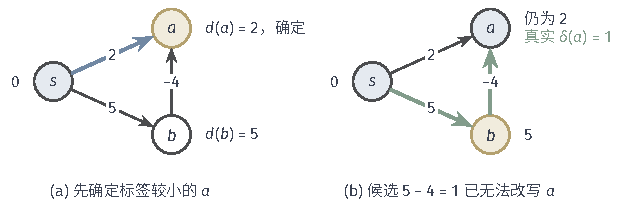
\includegraphics[width=105.583mm]{figures/01-basic-mathematics/04-graphs/tikz/c3-dijkstra-counterexample/figure.pdf}
  \caption{负边使Dijkstra算法过早确定标签。(a) 处理$s$后，$a$的标签$2$小于$b$的标签$5$，$a$被永久确定（黄色为当前出队顶点）。(b) 处理$b$时候选值$5-4=1$已无法改写$a$；真实最短路是$s\to b\to a$（绿色），成本$1$。图中没有负环，出错的原因是后半段弧$b\to a$为负。}
  \label{fig:graph-opt-dijkstra-counterexample}
\end{figure}

\paragraph{出队轨迹}
把四点图中$a\to b$的长度由$-1$改为$1$，全部弧长非负，Dijkstra算法适用。下面依次列出出队顶点与松弛结果：
\begin{enumerate}
  \item 取出$s$（标签$0$），松弛得$d(a)=2$、$d(b)=5$，前驱都是$s$；
  \item 取出$a$（标签$2$），候选$2+1=3<5$使$d(b)=3$、$p(b)=a$，候选$2+5=7$使$d(t)=7$、$p(t)=a$；
  \item 取出$b$（标签$3$），候选$3+2=5<7$使$d(t)=5$、$p(t)=b$；
  \item 取出$t$（标签$5$），没有出弧，队列为空。
\end{enumerate}
最终$\delta(a)=2$、$\delta(b)=3$、$\delta(t)=5$，从$t$沿前驱回溯得到$s\to a\to b\to t$。图~\ref{fig:graph-opt-dijkstra-trace}画出每次出队后的状态：已确定集合$R$逐个向外扩张，每个顶点在出队时的标签都不再改变。

\begin{figure*}[!htb]
  \centering
  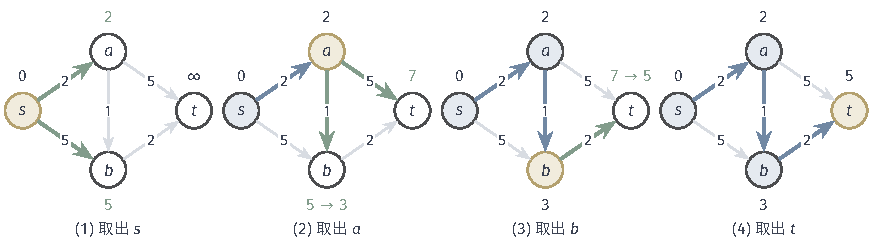
\includegraphics[width=147.687mm]{figures/01-basic-mathematics/04-graphs/tikz/c3-dijkstra-trace/figure.pdf}
  \caption{Dijkstra算法在非负四点图上的出队过程（$a\to b$长$1$，其余同前）。每个面板对应一次出队：蓝色为已确定顶点，黄色为本次出队的顶点，绿色标签与绿色弧表示本次松弛改善的标签及新前驱。四次出队依次确定$s=0$、$a=2$、$b=3$、$t=5$，最终前驱弧组成路线$s\to a\to b\to t$。}
  \label{fig:graph-opt-dijkstra-trace}
\end{figure*}

\paragraph{计算开销}
每个顶点至多出队一次，每条弧在其起点出队时松弛一次。用邻接表存储图、用支持降键的索引二叉堆存储未确定顶点时，取最小与降键各需$O(\log n)$时间，总时间为$O((n+a)\log n)$；标签、前驱、堆及其位置索引共占$O(n)$额外空间，图本身的存储另计。不降键的实现每次改善插入一个条目，堆中至多有$a+1$个条目，操作时间为$O(\log a)=O(\log n)$，总时间仍为$O((n+a)\log n)$，但队列空间上界变为$O(a)$。稠密图上也可以不用堆，每次扫描数组找最小标签，总时间为$O(n^2+a)$。

\subsection{方法比较与结果检验}
\label{sec:graph-opt-shortest-path-comparison}

三种算法解决同一个单源问题，但对输入的要求不同。比较它们时应先问：图有没有有向环？可达部分有没有负长度弧？是否需要检测负环？然后才比较运行时间。表~\ref{tab:graph-opt-shortest-path-methods}汇总了这些区别。

\begin{table}[!htb]
  \centering
  \caption{三种单源最短路算法的比较（$n$为顶点数，$a$为弧数，邻接表存储）。}
  \label{tab:graph-opt-shortest-path-methods}
  \begin{tabular}{llll}
    \toprule
    & 有向无环图递推 & Bellman--Ford & Dijkstra \\
    \midrule
    图结构 & 无有向环 & 不限 & 不限 \\
    弧长 & 任意实数 & 任意实数 & 可达部分非负 \\
    标签修正 & 处理后不变 & 反复修正 & 出队后不变 \\
    负环 & 不会出现 & 检测并标记 & 条件排除 \\
    时间 & $O(n+a)$ & $O(na)$ & $O((n+a)\log n)$ \\
    正确性依据 & 拓扑序归纳 & 至多$k$弧递推 & 首个未定顶点 \\
    \bottomrule
  \end{tabular}
\end{table}

“允许负边”与“存在负环”是两件不同的事。有向无环图递推与Bellman--Ford算法都允许负边；前者因为无环而不会遇到负环，后者则能在负环存在时正确报告受影响的顶点。Dijkstra算法连负边都不允许，哪怕负边并不构成负环，图~\ref{fig:graph-opt-dijkstra-counterexample}就是这样的例子。一种算法在某组数据上跑得更快、甚至答案碰巧正确，都不能替代对其条件的检查。

\paragraph{有限距离的检验}
拿到一份声称的最短路结果后，可以不重跑算法而直接核对。对标签有限的顶点，先沿前驱恢复路线，检查起点为$s$、终点为$v$、每一步都是原图中的弧，并重算弧长之和是否等于$d(v)$。这一步证明标签可以达到，即$d(v)\geq\delta(v)$。

最优性需要反方向的下界。若输出满足$d(s)=0$，并且对每条起点标签有限的弧$u\to v$都有
\[
  d(v)\leq d(u)+\ell_{u,v},
\]
那么任取一条$s$到$v$的行走$W=(s=w_0,w_1,\ldots,w_k=v)$，沿$W$把这些不等式逐条相加，中间标签相消，得到$d(v)\leq d(s)+\ell(W)=\ell(W)$。所以$d(v)\leq\delta(v)$，与可达性一起给出$d(v)=\delta(v)$。这组逐弧不等式只需$O(n+a)$时间核对，它本身就是有限距离的最优性证书；不满足时，违反不等式的弧直接指出了一条更好的路线。

\paragraph{不可达与负无穷的检验}
另外两类结果需要不同的证据。对报告为$+\infty$的顶点，用一次广度优先遍历核对它确实不在$s$的可达集中。对报告为$-\infty$的顶点，应给出三段证据：一条从$s$到某个有向环的行走、该环的成本为负，以及一条从环到该顶点的行走。三类结果各有各的验收方式，不能只核对其中一类就宣布整份结果正确。

% 第3章第2节：最小生成树（问题与最短路树的区别、割性质与安全选边、Kruskal、Prim、方法比较与结果检验）。

\section{最小生成树}
\label{sec:graph-minimum-spanning-tree}

要在若干城镇之间修路，使任意两个城镇都能互相到达，每条候选道路都有建造成本。这时关心的不是某两点之间怎样走最近，而是整张网络的总造价。第~\ref{sec:graph-trees-forests}节说明，连通且无环的边集恰好连接全部顶点而没有多余的边，即生成树；多一条边便形成环，环上任意一条边都可以拆掉而不破坏连通。于是问题化为：在所有生成树中找总边权最小的一棵。

本节先给出问题并与最短路区分，再建立割性质，它说明怎样的边可以放心地选入。Kruskal算法与Prim算法以不同的方式维护当前选边，但每一步都由割性质保证安全。最后在同一算例上比较两种算法，并区分“结果是一棵生成树”与“结果是最优的”这两种检查。

\subsection{最小生成树问题}
\label{sec:graph-opt-mst-problem}

设$\mathcal G=(V,E)$是有限无向连通图，每条边$e$带有实数权$w_e$，表示建造成本。对生成树$T\subseteq E$，记其总成本为$w(T)=\sum_{e\in T}w_e$。

\begin{definition}[最小生成树]
\label{def:graph-opt-mst}
有限无向连通加权图的所有生成树中，总成本$w(T)$最小者称为\term{最小生成树}（minimum spanning tree）。
\end{definition}

生成树只有有限多棵，所以最小生成树总是存在。它最小化的是连接全部顶点的总成本，并不保证树上每对顶点之间的路线都是原图中的最短路。图~\ref{fig:graph-opt-mst-vs-spt}中，三角形三条边的权为$w_{x,y}=2$、$w_{y,z}=2$、$w_{x,z}=3$。最小生成树取$\{xy,yz\}$，成本$4$；但在树上$x$到$z$要绕经$y$，长度为$4$，而原图中的直达边只有$3$。以$x$为源的\term{最短路树}（shortest-path tree），即由各顶点最短路的前驱弧组成的树，是$\{xy,xz\}$，成本$5$。两者回答不同的问题，一般不相同。同样，第~\ref{sec:graph-connectivity-computation}节由遍历得到的生成森林只保证连通与无环，不带有任何成本上的最优性。

\begin{figure}[!htb]
  \centering
  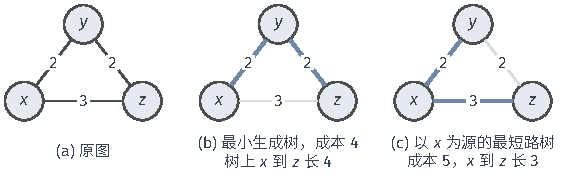
\includegraphics[width=95.793mm]{figures/01-basic-mathematics/04-graphs/tikz/c3-mst-vs-spt/figure.pdf}
  \caption{最小生成树与最短路树可以不同。(a) 原图，边旁为权。(b) 最小生成树$\{xy,yz\}$总成本$4$，但树上$x$到$z$的路线长$4$。(c) 以$x$为源的最短路树$\{xy,xz\}$保证每个顶点到$x$的距离最短，总成本却是$5$。蓝色粗边为所选的边。}
  \label{fig:graph-opt-mst-vs-spt}
\end{figure}

\paragraph{非连通、负权与平局}
图不连通时不存在生成树，问题改为在每个连通分量内分别求最小生成树，合起来称为\term{最小生成森林}（minimum spanning forest）。负权不会带来最短路那样的困难：每棵生成树恰有$n-1$条边，把所有边权同时加上常数$c$，每棵生成树的成本都增加$(n-1)c$，比较结果不变，因此总可以设想权都为正。边权有相同值时，最小生成树可能不止一棵，但最小总成本是唯一的。若要最大化总权，把全部边权取负即化为最小化问题，得到\term{最大生成树}（maximum spanning tree），下面的割性质与两种算法只需把“最小”改为“最大”即可照用。第~\ref{sec:graph-tree-decomposition-construction}节构造团树时会用到最大生成树。

\subsection{割性质与安全选边}
\label{sec:graph-opt-cut-property}

两种算法都是逐条选边，并希望每一步都不走错。“不走错”的确切含义是：当前已选的边集$A$总能扩充成某一棵最小生成树。只要保持这个不变量，选满$n-1$条边时，$A$本身就是一棵最小生成树。问题在于，下一条边选哪条才能保持不变量。

\paragraph{割与轻边}
把顶点集分成两个非空部分$S$与$V\setminus S$，称为图的一个\term{割}（cut），记作$(S,V\setminus S)$。一条边的两个端点分别在两侧时，称它跨越这个割。若已选边集$A$中没有边跨越该割，就称这个割与$A$相容。跨越某个割的边中权最小的称为该割的\term{轻边}（light edge），权相同时轻边可以不止一条。

\begin{lemma}[割性质]
\label{lem:graph-opt-cut-property}
设$\mathcal G$是有限无向连通加权图，边集$A$包含在某棵最小生成树中，割$(S,V\setminus S)$与$A$相容，$e$是该割的一条轻边。则$A\cup\{e\}$也包含在某棵最小生成树中。
\end{lemma}

\begin{proof}
取一棵包含$A$的最小生成树$T$。若$e\in T$，结论已成立。否则把$e$加入$T$，由第~\ref{sec:graph-trees-forests}节，树加一条边恰好形成一个环。设$e=\{u,v\}$，$u\in S$、$v\notin S$，这个环由$e$与$T$中$u$到$v$的路径组成。这条路径从$S$出发，最终到达$V\setminus S$，所以其中至少有一条边$f$跨越该割。

从$T+e$中删去$f$，环被打断，所得边集$T'=T+e-f$仍连通且有$n-1$条边，因而是生成树。由于$e$是轻边，$w_e\leq w_f$，所以$w(T')=w(T)+w_e-w_f\leq w(T)$，$T'$也是最小生成树。最后，割与$A$相容，跨越割的$f$不在$A$中，删去$f$不影响$A$；于是$A\cup\{e\}\subseteq T'$。
\end{proof}

图~\ref{fig:graph-opt-cut-exchange}画出这一交换：轻边$e$加入后与树中路径形成环，环上另一条跨割边$f$被删去，成本不增。

\begin{figure}[!htb]
  \centering
  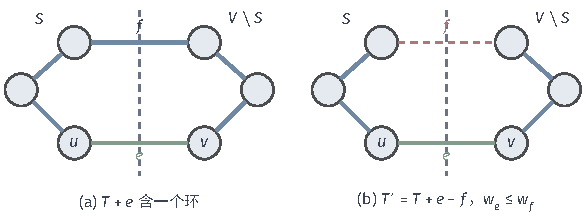
\includegraphics[width=99.187mm]{figures/01-basic-mathematics/04-graphs/tikz/c3-cut-exchange/figure.pdf}
  \caption{割性质的交换论证。虚线把顶点分成$S$与$V\setminus S$，蓝色粗边为最优树$T$，其中不跨割的边包含当前选边$A$。(a) 轻边$e$（绿色）不在$T$中，加入后与$T$中$u$到$v$的路径形成环。(b) 环上另一条跨割边$f$（红色虚线）被删去，得到$T'=T+e-f$，因$w_e\leq w_f$，成本不增。}
  \label{fig:graph-opt-cut-exchange}
\end{figure}

\paragraph{安全不等于必选}
割性质只保证轻边能留在\emph{某一棵}最优树中，并不保证它出现在\emph{每一棵}最优树中。设三角形三条边的权都是$1$，取割$(\{x\},\{y,z\})$，$xy$与$xz$都是轻边。最小生成树$\{xy,yz\}$不含$xz$，但按割性质选入$xz$仍然安全，因为$\{xz,yz\}$同样是最小生成树。平局时不同的选择通向不同的最优树，最优成本却相同。

割性质是两种算法的共同依据，区别只在于它们选取哪个割：Kruskal算法以当前森林中某个分量作为$S$，Prim算法以当前唯一一棵树的顶点集作为$S$。

\subsection{Kruskal算法}
\label{sec:graph-opt-kruskal}

一种自然的想法是从最便宜的边开始逐条考虑，只要不形成环就选入。开始时每个顶点自成一个分量；一条边的两端若属于不同分量，选入它会把两个分量连起来，不会成环；若两端已在同一分量，选入它就会成环，应当跳过。

\begin{algorithm}[Kruskal算法]
\label{alg:graph-opt-kruskal}
输入：有限无向加权图。输出：最小生成森林的边集$A$。状态：已选边集$A$与维护当前分量的并查集。
\begin{enumerate}
  \item 令$A=\varnothing$，为每个顶点建立一个单元素集合；把全部边按权从小到大排序，平局按固定的边序。
  \item 按排序依次取边$\{u,v\}$：若$u,v$的代表不同，把这条边加入$A$并合并两个集合；若代表相同，跳过。
  \item 选满$n-1$条边时可提前停止；否则扫描完全部边，输出的$A$是最小生成森林，集合个数即连通分量数。
\end{enumerate}
\end{algorithm}

判断两端是否属于同一分量、以及合并两个分量，正是第~\ref{sec:graph-connectivity-computation}节并查集的find与union操作。每选一条边，分量数减一且不产生环，所以选边数加分量数始终等于$n$。

\paragraph{算例}
取五个顶点$a,b,c,d,e$与七条边，权为$ab=1$、$bc=2$、$cd=3$、$ac=4$、$bd=5$、$ce=6$、$de=7$。按权依次考虑：$ab$、$bc$、$cd$的两端都属于不同分量，依次选入，此时分量为$\{a,b,c,d\}$与$\{e\}$，累计成本$6$；$ac$与$bd$的两端都已在$\{a,b,c,d\}$中，选入会成环，跳过；$ce$连接两个分量，选入后只剩一个分量，已选满$4=n-1$条边，停止。结果为$\{ab,bc,cd,ce\}$，总成本$1+2+3+6=12$。图~\ref{fig:graph-opt-kruskal-steps}画出了这一过程。这个图共有$21$棵生成树，逐一枚举可以核对成本$12$的只有这一棵，次优的成本为$13$。

\begin{figure}[!htb]
  \centering
  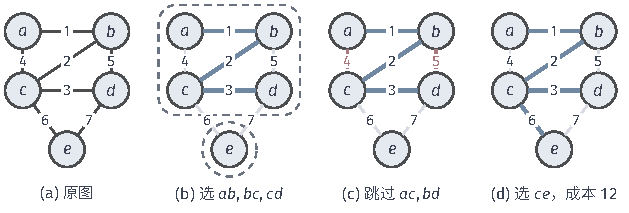
\includegraphics[width=106.5mm]{figures/01-basic-mathematics/04-graphs/tikz/c3-kruskal-steps/figure.pdf}
  \caption{Kruskal算法在五点七边图上的过程。(a) 原图，边旁为权。(b) 依次选入$ab,bc,cd$（蓝色粗边），虚线框标出当前分量$\{a,b,c,d\}$与$\{e\}$。(c) $ac$与$bd$的两端已在同一分量，选入会成环，跳过（红色虚线）。(d) 选入$ce$，得到最小生成树$\{ab,bc,cd,ce\}$，总成本$12$。}
  \label{fig:graph-opt-kruskal-steps}
\end{figure}

\paragraph{正确性}
下面用割性质说明Kruskal算法每次选入的边都是安全的。

\begin{theorem}[Kruskal算法的正确性]
\label{thm:graph-opt-kruskal}
对有限无向加权图，算法~\ref{alg:graph-opt-kruskal}输出一个最小生成森林；图连通时输出最小生成树。
\end{theorem}

\begin{proof}
先设图连通，证明不变量“$A$包含在某棵最小生成树中”。初始$A=\varnothing$，结论成立。设算法即将选入边$e=\{u,v\}$，取$S$为森林$(V,A)$中$u$所在的分量，则$v\notin S$，割$(S,V\setminus S)$与$A$相容。考察任意一条跨越这个割、权小于$w_e$的边$g$。它排在$e$之前，已被处理过：若当时被选入，它就在$A$中，而$A$中没有跨割的边；若当时被跳过，它的两端当时已在同一分量，分量只会合并而不会拆开，现在仍在同一分量，也不能跨割。所以跨越该割的边权都不小于$w_e$，$e$是轻边，由引理~\ref{lem:graph-opt-cut-property}，选入$e$后不变量仍成立。

扫描结束时，若原图中某条边连接了$(V,A)$的两个不同分量，处理到它时两端必属不同分量，它就会被选入，矛盾。所以$(V,A)$的分量与原图的分量相同，图连通时$A$是生成树。它包含在某棵最小生成树中，又与之边数相同，因而本身就是最小生成树。图不连通时，对每个分量分别应用上面的论证，结论对最小生成森林同样成立。
\end{proof}

\paragraph{计算开销}
排序需要$O(m\log m)$时间。之后至多处理$m$条边，每条边做两次find，选入时再做一次union，共$O(m)$次并查集操作。采用第~\ref{sec:graph-connectivity-computation}节的按大小合并时，树高不超过$O(\log n)$，每次操作$O(\log n)$，这部分为$O(m\log n)$；由于$m\leq n^2$，$\log m\leq2\log n$，总时间为$O(m\log n)$，空间为边表与并查集的$O(n+m)$。若再配合路径压缩，并查集操作的摊还开销几乎为常数，此时排序成为主要开销。算法的正确性只依赖割性质，与并查集采用哪种实现无关。

\subsection{Prim算法}
\label{sec:graph-opt-prim}

Kruskal算法同时维护许多分量，按全局次序选边。另一种做法是只让一棵树生长：从一个顶点出发，每次把一个外部顶点用最便宜的边接到树上。

\paragraph{键与算法步骤}
为每个尚未入树的顶点$v$记录一个键$\operatorname{key}(v)$，表示$v$与当前树之间最便宜的边的权，同时记录这条边在树内的端点$p(v)$。这里的键是\emph{一条}连接边的权，不是Dijkstra算法中从源点出发的累计长度。

\begin{algorithm}[Prim算法]
\label{alg:graph-opt-prim}
输入：有限无向连通加权图、起点$r$。输出：最小生成树的边集。状态：树的顶点集$S$、外部顶点的键与父点、按键排序的优先队列。
\begin{enumerate}
  \item 令$S=\{r\}$；对$r$的每个邻居$v$，令$\operatorname{key}(v)=w_{r,v}$、$p(v)=r$，其余外部顶点的键为$+\infty$。
  \item 当$S\neq V$时，取出键最小的外部顶点$u$，把$u$加入$S$，把边$\{p(u),u\}$加入树。
  \item 对$u$的每个外部邻居$v$，若$w_{u,v}<\operatorname{key}(v)$，令$\operatorname{key}(v)=w_{u,v}$、$p(v)=u$。
\end{enumerate}
\end{algorithm}

第三步之后，每个外部顶点的键仍等于它与$S$中顶点之间最便宜的边权：新加入的$u$只带来了从$u$出发的边，逐一比较即可。因此每次取出的最小键对应的边，正是割$(S,V\setminus S)$的一条轻边。

\paragraph{算例}
在与Kruskal算法相同的五点图上从$a$出发，过程如图~\ref{fig:graph-opt-prim-steps}。开始时$\operatorname{key}(b)=1$、$\operatorname{key}(c)=4$。取出$b$，选入$ab$；$b$的邻边把$c$的键从$4$改为$2$，并给$d$设键$5$。取出$c$，选入$bc$；$d$的键从$5$改为$3$，$e$得到键$6$。取出$d$，选入$cd$；$de=7$不优于$e$现有的键$6$，不更新。最后取出$e$，选入$ce$。所得的树与Kruskal算法相同，成本$12$。

\begin{figure*}[!htb]
  \centering
  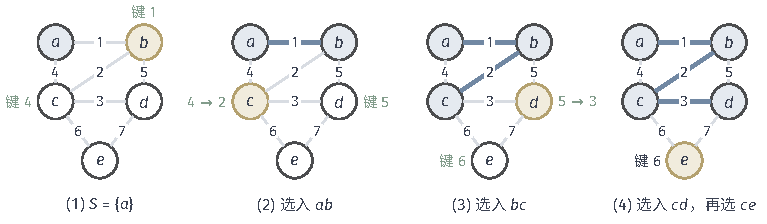
\includegraphics[width=129.858mm]{figures/01-basic-mathematics/04-graphs/tikz/c3-prim-steps/figure.pdf}
  \caption{Prim算法从$a$出发的过程。每个面板中蓝色顶点与蓝色粗边是当前树，外部顶点旁标出键，绿色表示刚被改善的键，黄色为下一个取出的顶点。依次选入$ab,bc,cd,ce$，各步加入的边恰是当前树顶点集所形成割的轻边；最终的树与Kruskal算法相同，成本$12$。}
  \label{fig:graph-opt-prim-steps}
\end{figure*}

换一个起点，选边次序会变。从$e$出发时，$c$与$d$的键分别为$6$与$7$；先选入$ec=6$，$c$的邻边使$b$、$a$、$d$的键变为$2$、$4$、$3$；再选入$cb=2$，$a$的键降为$1$；随后选入$ba=1$与$cd=3$。所选边权依次为$6,2,1,3$，并不递增。这与Kruskal算法的全局排序不同：Prim算法每次只在当前割上取最轻的边，不同时刻面对的是不同的割。

\paragraph{正确性}
正确性同样来自割性质：令$A$为当前树的边集，$S$为其顶点集。$A$的边都在$S$内部，割$(S,V\setminus S)$与$A$相容；算法选入的边是该割的轻边，由引理~\ref{lem:graph-opt-cut-property}，若$A$包含在某棵最小生成树中，加入新边后仍然如此。从$A=\varnothing$出发归纳，选满$n-1$条边时得到最小生成树。

\paragraph{实现与开销}
用数组保存键、每次线性扫描找最小时，$n$次取最小共$O(n^2)$，每条边至多引起一次键的比较与更新，总时间为$O(n^2+m)$，适合稠密图。用支持降键的索引二叉堆时，取最小与降键各需$O(\log n)$，总时间为$O((n+m)\log n)$，适合稀疏图。两种实现的额外空间都是$O(n)$。图不连通时，一棵树长满所在分量后，从任一尚未访问的顶点重新开始，得到最小生成森林，各分量的父边与成本分别保留。

\subsection{方法比较与结果检验}
\label{sec:graph-opt-mst-comparison}

两种算法读取边与维护状态的方式不同。Kruskal算法一次性对全部边排序，按全局次序检查，用并查集维护多个分量，适合边已经以列表形式给出的稀疏图。Prim算法从一棵树出发，只读取新入树顶点的邻边，用键数组或堆维护局部信息，在用邻接矩阵存储的稠密图上，数组版本的$O(n^2)$开销已与读入图的开销同阶。孰优孰劣取决于图的稠密程度、边的组织方式和所用数据结构，不能只凭算法名称判断。

\paragraph{可行性与最优性}
检验一份声称的最小生成森林时，先确认它是一个可行的生成森林：所选的每条边都来自原图；每个原连通分量的顶点都被覆盖；所选边无环，可以用并查集逐条加入核对；选边数等于$n$减去分量数。然后重算总成本。这些检查只证明结果是\emph{一个}生成森林，不能证明它最优。

最优性要回到割性质与算法的交换论证。一种可以独立执行的检查是：对每条未被选中的边$\{u,v\}$，考察树上$u$到$v$的路径，若路径上有一条边的权大于$w_{u,v}$，用这条非树边替换它，就得到成本更低的生成树，结果必不最优。反过来，若每条非树边都不轻于它在树上对应路径中的每条边，这棵树就是最优的；这一充分性可以仿照割性质的交换论证证明，这里从略。小规模的例子还可以枚举全部生成树作对照，如前面的五点图。但两种算法在某个例子上给出相同的树，只是一致性的旁证，不能当作一般正确性的证明。

% 第3章第3节：最大流与最小割（流、容量与割；残量网络；增广路径与最优性条件；Ford--Fulkerson增广法；Edmonds--Karp算法；算法分析与结果检验）。

\section{最大流与最小割}
\label{sec:graph-max-flow}

前两节各选出一个结构：一条路线或一棵树。现在设想从水厂向用户输水，每段管道有输送上限，水可以同时沿多条管道并行，也可以在中途汇合、分流。要回答的是单位时间内最多能送出多少水。这次选择的对象不是一条路径，而是每条弧上的一个流量，所有流量要同时满足容量上限和中途不积存的条件。两条路线若共用一段容量为$1$的管道，它们合计只能送$1$，不能各送$1$。

本节先建立流、容量与割，并证明任何流量都不超过任何割的容量。为了改进当前的输送方案，引入允许撤回旧流量的残量网络，由此得到判断一个流是否最优的增广路径判据，以及与之同值的割证书。随后介绍两种算法：Ford--Fulkerson方法任意选取增广路径，在整数容量下有限终止；Edmonds--Karp算法规定按最少弧数选路，对任意实容量都有与数值无关的增广次数界，并由此得到最大流最小割定理。

\subsection{流、容量与割}
\label{sec:graph-opt-flow-cut}

设$\mathcal G=(V,E)$是有限有向图，指定两个不同的顶点：源点$s$与汇点$t$。每条弧$u\to v$带有有限非负实数\emph{容量}$c_{u,v}$，表示该弧单位时间内最多能通过的量。这样的四元组$(\mathcal G,c,s,t)$称为\term{流网络}（flow network）。

\begin{definition}[流与流值]
\label{def:graph-opt-flow}
流网络上的一个\term{流}（flow）是给每条弧$u\to v$赋予实数$x_{u,v}$的一组数$\bm x=(x_{u,v})$，满足
\begin{gather}
  0\leq x_{u,v}\leq c_{u,v}\quad\text{对每条弧}\ u\to v,\label{eq:graph-opt-capacity}\\
  \sum_{u:\,u\to v}x_{u,v}=\sum_{w:\,v\to w}x_{v,w}\quad\text{对每个}\ v\in V\setminus\{s,t\}.\label{eq:graph-opt-conservation}
\end{gather}
前者称为容量约束，后者称为\term{流守恒}（flow conservation）。源点的净流出
\[
  \operatorname{val}(\bm x)=\sum_{w:\,s\to w}x_{s,w}-\sum_{u:\,u\to s}x_{u,s}
\]
称为\term{流值}（flow value）。流值最大的流称为\term{最大流}（maximum flow）。
\end{definition}

流守恒说明中间顶点只转运、不积存，所以源点送出的净量应该全部到达汇点。为验证这一点，对每个顶点计算净流出（流出减流入）并对全部顶点求和：每条弧的流量在起点算一次正、在终点算一次负，总和为零。中间顶点的净流出都是零，于是源点的净流出等于汇点的净流入，即$\operatorname{val}(\bm x)$也是$t$收到的净量。流值不是全图各弧流量的总和：一单位流量经过三条弧到达汇点，只算一单位流值。

\paragraph{割与割容量}
为了估计流值能有多大，把顶点分成包含$s$的一侧$S$与包含$t$的一侧$\bar S=V\setminus S$，称$(S,\bar S)$为一个$s$--$t$割。这里沿用第~\ref{sec:graph-opt-cut-property}节割的含义，只是额外要求源、汇分居两侧。割的\term{割容量}（cut capacity）只累计从源侧跨向汇侧的弧：
\[
  c(S,\bar S)=\sum_{u\in S,\ v\in\bar S,\ u\to v}c_{u,v}.
\]
从汇侧指回源侧的弧不计入容量。直观上，任何从$s$到$t$的输送都要穿过这个割，穿过的总量不可能超过这些弧的容量之和。下面把这一直观变成证明。

\begin{lemma}[流值不超过割容量]
\label{lem:graph-opt-weak-duality}
对任意流$\bm x$与任意$s$--$t$割$(S,\bar S)$，有
\begin{equation}
  \operatorname{val}(\bm x)=\sum_{u\in S,\,v\in\bar S}x_{u,v}-\sum_{v\in\bar S,\,u\in S}x_{v,u}\leq c(S,\bar S).
  \label{eq:graph-opt-net-flow-cut}
\end{equation}
\end{lemma}

\begin{proof}
对$S$中的全部顶点把净流出相加。$s$贡献$\operatorname{val}(\bm x)$，其余顶点都是中间顶点（$t\notin S$），贡献为零，所以和等于$\operatorname{val}(\bm x)$。另一方面，两端都在$S$内的弧在起点计正、在终点计负，相互抵消；剩下的只有跨割的弧：从$S$指向$\bar S$的弧计正，从$\bar S$指回$S$的弧计负。这就得到式~\eqref{eq:graph-opt-net-flow-cut}中的等式。再由容量约束，第一个和不超过$c(S,\bar S)$，第二个和不小于零，得到不等式。
\end{proof}

式~\eqref{eq:graph-opt-net-flow-cut}说明，流值等于跨过任意一个割的净流量，而每个割的容量都是流值的上界。图~\ref{fig:graph-opt-flow-network-cut}中，取$S=\{s,b\}$，跨出的弧$s\to a$与$b\to t$容量合计$6$，指回的弧$a\to b$不计入；所示流在这两条弧上分别送$3$与$3$，在$a\to b$上送回$1$，净流量$3+3-1=5$恰为流值，不超过割容量$6$。

\begin{figure}[!htb]
  \centering
  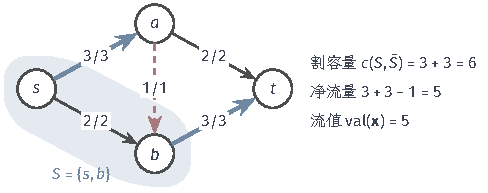
\includegraphics[width=82.564mm]{figures/01-basic-mathematics/04-graphs/tikz/c3-flow-network-cut/figure.pdf}
  \caption{流网络、流与割。弧旁的“$x/c$”表示流量与容量，每个中间顶点流入等于流出，流值为$5$。浅色底标出割的源侧$S=\{s,b\}$：跨出的弧$s\to a$、$b\to t$（蓝色粗弧）的容量计入割容量$3+3=6$；指回的弧$a\to b$（红色虚线）不计容量，其流量在净流量中扣除，$3+3-1=5$。}
  \label{fig:graph-opt-flow-network-cut}
\end{figure}

\subsection{残量网络}
\label{sec:graph-opt-residual-network}

最朴素的改进办法是：找一条从$s$到$t$、每条弧都还有剩余容量的路径，沿它多送一些。但已经选定的路线可能占用了更好的安排，只会追加流量的办法会过早卡住。下面的例子会说明这一点，补救的办法是允许撤回一部分旧流量，把撤回也当作一种可以使用的“通道”。

\paragraph{正向残量与反向残量}
给定流$\bm x$，对每条原弧$u\to v$建立两条\emph{残量弧}：正向残量弧$u\to v$，容量$c_{u,v}-x_{u,v}$，表示还能追加多少；反向残量弧$v\to u$，容量$x_{u,v}$，表示能撤回多少。只保留容量为正的残量弧，得到的有向图称为\term{残量网络}（residual network），记作$\mathcal G_{\bm x}$，残量弧的容量记作$r_{\bm x}$。例如原弧容量为$3$、当前流量为$2$时，正向残量为$1$、反向残量为$2$，如图~\ref{fig:graph-opt-residual-arc}。沿反向残量弧$v\to u$送出一单位，含义是把原弧$u\to v$上的流量减少一单位，并不要求原网络中真有一条从$v$到$u$的管道。

\begin{figure}[!htb]
  \centering
  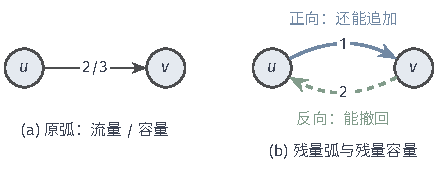
\includegraphics[width=74.186mm]{figures/01-basic-mathematics/04-graphs/tikz/c3-residual-arc/figure.pdf}
  \caption{一条原弧对应两条残量弧。(a) 原弧$u\to v$容量$3$、流量$2$。(b) 残量网络中，正向残量弧$u\to v$（蓝色）容量$3-2=1$，表示还能追加的量；反向残量弧$v\to u$（绿色虚线）容量$2$，表示能撤回的量。流量为$0$时没有反向残量弧，满流时没有正向残量弧。}
  \label{fig:graph-opt-residual-arc}
\end{figure}

\paragraph{撤回旧流的例子}
取弧$s\to a$、$s\to b$、$a\to b$、$a\to t$、$b\to t$，容量都为$1$。若先沿$s\to a\to b\to t$送一单位，三条弧都满了，剩下的$s\to b$与$a\to t$虽有空余，却连不成一条只用正向残量的$s$--$t$路径，只会追加的办法到此停止，流值为$1$。但残量网络中还有反向残量弧$b\to a$，容量$1$，于是出现路径$s\to b\to a\to t$：在$s\to b$与$a\to t$上各追加一单位，同时把$a\to b$上的流量撤回一单位。更新后的流在$s\to a$、$a\to t$、$s\to b$、$b\to t$上各为$1$，在$a\to b$上为$0$，流值为$2$。逐点核对：$a$流入$1$、流出$1$，$b$流入$1$、流出$1$，各弧都不超过容量。图~\ref{fig:graph-opt-undo-flow}画出这三个阶段。最终的实际输送是两条不相交的路线$s\to a\to t$与$s\to b\to t$，第一次选路时经过$a\to b$的那一单位被“改道”了。

\begin{figure*}[!htb]
  \centering
  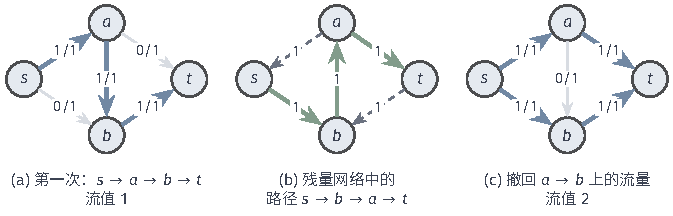
\includegraphics[width=113.901mm]{figures/01-basic-mathematics/04-graphs/tikz/c3-undo-flow/figure.pdf}
  \caption{单位容量网络中撤回旧流量。(a) 先沿$s\to a\to b\to t$送一单位（蓝色粗弧为流量$1$的弧），只用正向残量已无$s$--$t$路径。(b) 残量网络：满流弧只剩反向残量弧（灰色），绿色路径$s\to b\to a\to t$经过反向残量弧$b\to a$。(c) 沿该路径更新后，$a\to b$上的流量被撤回，流值变为$2$，实际路线为$s\to a\to t$与$s\to b\to t$。}
  \label{fig:graph-opt-undo-flow}
\end{figure*}

原网络若同时有$u\to v$与$v\to u$两条弧，残量网络中可能出现两条同向的$u\to v$残量弧：一条是原弧$u\to v$的正向残量，另一条是原弧$v\to u$的反向残量。实现时应保留每条残量弧对应哪条原弧、哪个方向的身份，沿它送流时修改的是对应原弧的流量。否则会把“真实地反向输送”与“撤回另一条弧上的流量”混成同一个量。

\subsection{增广路径与最优性条件}
\label{sec:graph-opt-augmenting-path}

有了残量网络，改进一个流的办法就统一成了找路：残量网络中的任何一条$s$--$t$路径都给出一种在不违反约束的前提下增加流值的调整。

\paragraph{增广路径与瓶颈}
残量网络$\mathcal G_{\bm x}$中从$s$到$t$的简单路径$P$称为关于$\bm x$的\term{增广路径}（augmenting path）。$P$上残量容量的最小值
\[
  \Delta=\min_{(u\to v)\in P}r_{\bm x}(u,v)>0
\]
称为$P$的\term{瓶颈容量}（bottleneck capacity）。沿$P$增广$\Delta$，是指对$P$上的每条残量弧：若它是原弧$u\to v$的正向残量，令$x_{u,v}\leftarrow x_{u,v}+\Delta$；若它是原弧$v\to u$的反向残量，令$x_{v,u}\leftarrow x_{v,u}-\Delta$。

\begin{lemma}[沿增广路径更新保持可行]
\label{lem:graph-opt-augment}
设$\bm x$是流，$P$是增广路径，瓶颈容量为$\Delta$。沿$P$增广$\Delta$后得到的$\bm x'$仍是流，并且$\operatorname{val}(\bm x')=\operatorname{val}(\bm x)+\Delta$。
\end{lemma}

\begin{proof}
容量约束：正向残量弧满足$\Delta\leq c_{u,v}-x_{u,v}$，追加后不超过容量；反向残量弧满足$\Delta\leq x_{v,u}$，撤回后不小于零。流守恒：$P$是简单路径，经过每个中间顶点$v$恰好一次，一条残量弧进入$v$，一条离开$v$。进入的那条若是正向残量，$v$的流入增加$\Delta$；若是反向残量，即撤回一条从$v$出发的原弧上的流量，$v$的流出减少$\Delta$。两种情形都使$v$的净流出减少$\Delta$。同理，离开的那条残量弧使$v$的净流出增加$\Delta$。两者相抵，$v$仍满足守恒。最后，$P$的第一条残量弧离开$s$，使$s$的净流出增加$\Delta$，而$P$是简单路径，不再回到$s$，所以流值增加$\Delta$。
\end{proof}

\paragraph{同值割证书}
引理说明，只要存在增广路径，当前流就不是最大流。反过来，没有增广路径时，能否断定当前流最大？答案是肯定的，而且可以从残量网络中直接读出一个与流值相等的割。

\begin{theorem}[增广路径判据]
\label{thm:graph-opt-augmenting-path}
设$\bm x$是流网络上的一个流，则下列三条等价：
\begin{enumerate}
  \item $\bm x$是最大流；
  \item 残量网络$\mathcal G_{\bm x}$中不存在增广路径；
  \item 存在某个$s$--$t$割$(S,\bar S)$，使$\operatorname{val}(\bm x)=c(S,\bar S)$。
\end{enumerate}
此时$(S,\bar S)$是割容量最小的$s$--$t$割，可取$S$为$\mathcal G_{\bm x}$中从$s$可达的顶点集。
\end{theorem}

\begin{proof}
由1推2：若存在增广路径，由引理~\ref{lem:graph-opt-augment}可得流值更大的流，与$\bm x$最大矛盾。

由2推3：令$S$为$\mathcal G_{\bm x}$中从$s$可达的顶点集。$s\in S$，而没有增广路径说明$t\notin S$，所以$(S,\bar S)$是$s$--$t$割。考察跨割的原弧。若$u\in S$、$v\in\bar S$且$u\to v$是原弧，则必有$x_{u,v}=c_{u,v}$，否则正向残量弧$u\to v$存在，$v$就从$s$可达了。若$v\in\bar S$、$u\in S$且$v\to u$是原弧，则必有$x_{v,u}=0$，否则反向残量弧$u\to v$存在，同样使$v$可达。把这两条代入式~\eqref{eq:graph-opt-net-flow-cut}，第一个和等于$c(S,\bar S)$，第二个和为零，故$\operatorname{val}(\bm x)=c(S,\bar S)$。

由3推1：对任意流$\bm y$，引理~\ref{lem:graph-opt-weak-duality}给出$\operatorname{val}(\bm y)\leq c(S,\bar S)=\operatorname{val}(\bm x)$，所以$\bm x$最大。同一不等式对任意割$(S',\bar S')$给出$c(S',\bar S')\geq\operatorname{val}(\bm x)=c(S,\bar S)$，所以$(S,\bar S)$的割容量最小。
\end{proof}

割容量最小的$s$--$t$割称为\term{最小割}（minimum cut）。定理把“是否最优”这个关于全部候选流的问题，化成了在残量网络中做一次遍历就能回答的问题；停止时得到的流与割互为证书，任何人都可以逐弧核对两者的数值相等，而不必相信算法本身。图~\ref{fig:graph-opt-max-flow-certificate}是第~\ref{sec:graph-opt-flow-cut}小节网络的一个最大流及其证书：残量网络中$s$的两条出弧都已满流，从$s$出发哪里也去不了，$S=\{s\}$，割容量$3+2=5$等于流值。

\begin{figure}[!htb]
  \centering
  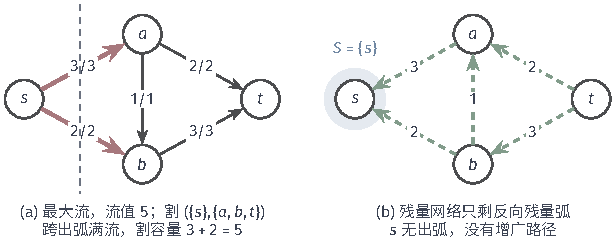
\includegraphics[width=104.186mm]{figures/01-basic-mathematics/04-graphs/tikz/c3-max-flow-certificate/figure.pdf}
  \caption{最大流与最小割互为证书。(a) 原网络上的最大流，弧旁为“流量/容量”，流值为$5$；虚线表示割$(\{s\},\{a,b,t\})$，其跨出弧$s\to a$、$s\to b$（红色）均满流，割容量$3+2=5$等于流值。(b) 对应的残量网络：五条原弧都已满流，只剩反向残量弧（绿色虚线），弧旁为残量容量；$s$没有出弧，从$s$可达的集合为$S=\{s\}$（浅色底），不存在增广路径。}
  \label{fig:graph-opt-max-flow-certificate}
\end{figure}

需要注意定理的范围。它判定一个\emph{给定}的流是否最优，并在最优时给出证书；它没有断言任意选路的增广过程一定会在有限步内走到这样的流，也还没有说明最大流一定存在。存在性由第~\ref{sec:graph-opt-edmonds-karp}小节的Edmonds--Karp算法以构造的方式补齐。

\subsection{Ford--Fulkerson增广法}
\label{sec:graph-opt-ford-fulkerson}

定理~\ref{thm:graph-opt-augmenting-path}直接给出一个算法框架：从零流出发，只要残量网络中还有增广路径就沿它增广，没有时停止。这个框架称为\term{Ford--Fulkerson方法}（Ford--Fulkerson method）。称它为“方法”，是因为它没有规定选哪条增广路径。

\begin{algorithm}[Ford--Fulkerson增广法]
\label{alg:graph-opt-ford-fulkerson}
输入：流网络$(\mathcal G,c,s,t)$。输出：流$\bm x$与割$(S,\bar S)$。状态：各原弧的流量、由流量确定的正反残量、搜索用的前驱与当前流值。
\begin{enumerate}
  \item 令$\bm x=\bm 0$。
  \item 在当前残量网络中搜索一条$s$--$t$路径，记录前驱；若没有，转第4步。
  \item 沿前驱恢复路径$P$，求瓶颈$\Delta$，按引理~\ref{lem:graph-opt-augment}更新对应原弧的流量，流值加$\Delta$，回到第2步。
  \item 令$S$为最后一次搜索中从$s$可达的顶点集，输出$\bm x$与$(S,\bar S)$。
\end{enumerate}
\end{algorithm}

每次更新都会改变若干残量：正向残量减少，反向残量增加，有的残量弧消失，也有新的出现。所以每轮都要在更新后的残量网络中重新搜索，不能沿用上一轮找到的其他路径。

\paragraph{算例}
回到图~\ref{fig:graph-opt-flow-network-cut}的网络，弧$s\to a$、$s\to b$、$a\to b$、$a\to t$、$b\to t$的容量依次为$3,2,1,2,3$。从零流出发：
\begin{enumerate}
  \item 沿$s\to a\to t$增广，瓶颈$\min\{3,2\}=2$，流值为$2$；
  \item 沿$s\to b\to t$增广，瓶颈$\min\{2,3\}=2$，流值为$4$；
  \item 此时$s\to a$剩余$1$，$a\to t$已满，沿$s\to a\to b\to t$增广，瓶颈$\min\{1,1,1\}=1$，流值为$5$。
\end{enumerate}
所得流在五条弧上依次为$3,2,1,2,3$，每条弧都满流。$a$流入$3$、流出$1+2=3$，$b$流入$2+1=3$、流出$3$，守恒成立。残量网络中$s$的两条出弧都已饱和，搜索停止，得到$S=\{s\}$，即图~\ref{fig:graph-opt-max-flow-certificate}中的证书。前面的单位容量例子也是这个框架的一次运行：先选了$s\to a\to b\to t$，第二轮的增广路径$s\to b\to a\to t$经过反向残量弧，撤回了旧的流量。

\paragraph{整数容量下的有限终止}
框架是否总会停止？容量都是整数时，答案是肯定的。

\begin{theorem}[整数容量下的有限终止]
\label{thm:graph-opt-integer-termination}
若所有容量都是非负整数，则Ford--Fulkerson方法无论怎样选择增广路径，至多经过$C_s=\sum_{w:\,s\to w}c_{s,w}$次增广就停止，输出的流是最大流，并且每条弧上的流量都是整数。
\end{theorem}

\begin{proof}
对增广次数归纳可知，流量始终是整数：零流是整数的；若当前流量都是整数，则残量$c_{u,v}-x_{u,v}$与$x_{u,v}$都是整数，瓶颈$\Delta$是正整数，更新后流量仍为整数。于是每次增广使流值至少增加$1$。另一方面，由引理~\ref{lem:graph-opt-weak-duality}，取$S=\{s\}$可知流值不超过$C_s$。所以增广至多$C_s$次。停止时没有增广路径，由定理~\ref{thm:graph-opt-augmenting-path}，所得流最大。
\end{proof}

这个定理同时说明，整数容量的网络存在每条弧流量都为整数的最大流，第~\ref{sec:graph-matching}节的匹配会用到这一点。容量为有理数时，乘以公分母即化为整数情形。但对一般的实容量，上面的整数步长论证不能照搬：每次流值都增加，增加量却可能越来越小。已知存在容量含无理数的网络，任意选路的Ford--Fulkerson方法可以永不停止，流值甚至收敛到小于最大流值的数。因此，任意选路的框架不自动具有有限终止的保证，需要对选路规则加以限制。

\subsection{Edmonds--Karp算法}
\label{sec:graph-opt-edmonds-karp}

Edmonds--Karp算法保留残量网络与增广更新，只对选路加一条规则：每次用广度优先遍历寻找弧数最少的增广路径。这里的“最短”按残量弧的条数计算，容量不参与路径长短的比较。

\begin{algorithm}[Edmonds--Karp算法]
\label{alg:graph-opt-edmonds-karp}
与算法~\ref{alg:graph-opt-ford-fulkerson}相同，只是第2步固定用第~\ref{sec:graph-bfs}节的广度优先遍历在残量网络中从$s$搜索，所得前驱路径是弧数最少的$s$--$t$路径。
\end{algorithm}

\paragraph{算例}
在同一个$3,2,1,2,3$网络上按字母顺序访问邻居，记$h(v)$为$v$在当前残量网络中的广度优先层数，即从$s$出发的最少弧数。第$1$轮，各层为$h(a)=h(b)=1$、$h(t)=2$，选出$s\to a\to t$，瓶颈$2$。第$2$轮，残量网络中$s\to a$剩$1$、$a\to t$已满，层数仍为$h(a)=h(b)=1$、$h(t)=2$，选出$s\to b\to t$，瓶颈$2$。第$3$轮，$s\to b$已满，$b$只能经$a$到达，层数变为$h(a)=1$、$h(b)=2$、$h(t)=3$，选出$s\to a\to b\to t$，瓶颈$1$。第$4$轮从$s$出发不能到达任何顶点，停止，流值为$5$。图~\ref{fig:graph-opt-edmonds-karp-layers}画出各轮的残量网络与分层。

\begin{figure*}[!htb]
  \centering
  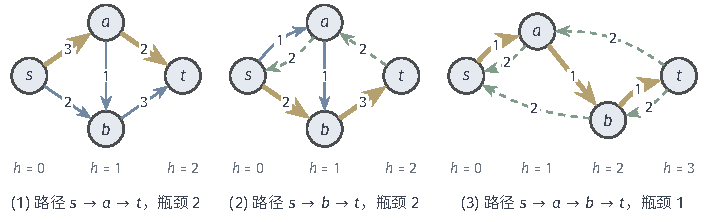
\includegraphics[width=119.567mm]{figures/01-basic-mathematics/04-graphs/tikz/c3-edmonds-karp-layers/figure.pdf}
  \caption{Edmonds--Karp算法在$3,2,1,2,3$网络上的三轮增广。每个面板是该轮开始时的残量网络，顶点按广度优先层数$h$从左到右排列，弧旁为残量容量，蓝色为正向残量弧，绿色虚线为反向残量弧；黄色粗箭头是本轮选出的弧数最少的增广路径。汇点层数依次为$2,2,3$，不随增广而减小。}
  \label{fig:graph-opt-edmonds-karp-layers}
\end{figure*}

这个网络上，Edmonds--Karp算法选出的路径恰好与前面手工选择的相同。差别在单位容量的例子中显现：任意选路时可以先选三条弧的$s\to a\to b\to t$，随后不得不撤回；Edmonds--Karp算法第一轮只会选两条弧的$s\to a\to t$，第二轮选$s\to b\to t$，两次增广即达到流值$2$，不需要撤回。

\paragraph{层数不下降}
增广次数的上界来自层数的变化。记$h_{\bm x}(v)$为$v$在$\mathcal G_{\bm x}$中从$s$出发的最少弧数，不可达时为$+\infty$。首先证明，沿最短增广路径增广不会让任何顶点离$s$更近。

\begin{lemma}[残量层数单调不减]
\label{lem:graph-opt-levels-monotone}
设$\bm x'$由$\bm x$沿$\mathcal G_{\bm x}$中一条弧数最少的增广路径增广得到，则对每个顶点$v$都有$h_{\bm x'}(v)\geq h_{\bm x}(v)$。
\end{lemma}

\begin{proof}
假设结论不成立，在所有满足$h_{\bm x'}(v)<h_{\bm x}(v)$的顶点中取$h_{\bm x'}(v)$最小的一个$v$。显然$v\neq s$。取$\mathcal G_{\bm x'}$中一条$s$到$v$的最短路径，设其最后一条弧为$u\to v$，则$h_{\bm x'}(u)=h_{\bm x'}(v)-1$；由$v$的最小性，$h_{\bm x'}(u)\geq h_{\bm x}(u)$。分两种情形。

若弧$u\to v$在增广前已在$\mathcal G_{\bm x}$中，则$h_{\bm x}(v)\leq h_{\bm x}(u)+1\leq h_{\bm x'}(u)+1=h_{\bm x'}(v)$，与假设矛盾。

若$u\to v$在增广前不在$\mathcal G_{\bm x}$中，它是增广新产生的残量弧。增广只会让路径上残量弧的反向弧获得正容量，所以$v\to u$在增广路径上。增广路径是弧数最少的路径，路径上相邻顶点的层数相差一，故$h_{\bm x}(u)=h_{\bm x}(v)+1$。于是$h_{\bm x}(v)=h_{\bm x}(u)-1\leq h_{\bm x'}(u)-1=h_{\bm x'}(v)-2$，同样矛盾。
\end{proof}

\paragraph{增广次数的上界}
每次增广中，瓶颈弧的残量降为零，从残量网络中消失，称它在这次增广中\emph{饱和}。下面说明同一条残量弧不能频繁地饱和。

\begin{theorem}[Edmonds--Karp算法的增广次数]
\label{thm:graph-opt-edmonds-karp}
在有限实容量的流网络上，Edmonds--Karp算法至多进行$na$次增广就停止。
\end{theorem}

\begin{proof}
残量弧按其对应的原弧与方向区分，至多有$2a$条。固定其中一条$u\to v$。它在某次增广中饱和时位于最短增广路径上，所以$h_{\bm x}(v)=h_{\bm x}(u)+1$，随后从残量网络中消失。它要再次出现，必须在之后的某次增广中，反向弧$v\to u$位于当时的增广路径上，设当时的流为$\bm x''$，则$h_{\bm x''}(u)=h_{\bm x''}(v)+1$。由引理~\ref{lem:graph-opt-levels-monotone}，层数不下降，所以
\[
  h_{\bm x''}(u)=h_{\bm x''}(v)+1\geq h_{\bm x}(v)+1=h_{\bm x}(u)+2.
\]
也就是说，$u\to v$相邻两次饱和之间，$u$的层数至少增加$2$。$u$作为增广路径上的非汇点顶点，其层数在$0$到$n-2$之间，因此$u\to v$至多饱和$n/2$次。每次增广至少饱和一条残量弧，总增广次数不超过$2a\cdot n/2=na$。
\end{proof}

这个界只依赖顶点数与弧数，与容量的数值无关，所以对任意有限实容量都成立。算法停止时没有增广路径，由定理~\ref{thm:graph-opt-augmenting-path}，所得流最大，残量可达集给出最小割。这就以构造的方式证明了最大流的存在，并得到本节的核心结论。

\begin{theorem}[最大流最小割定理]
\label{thm:graph-opt-max-flow-min-cut}
在有限非负实容量的流网络中，最大流存在，并且最大流值等于最小$s$--$t$割的割容量。
\end{theorem}

\begin{proof}
由定理~\ref{thm:graph-opt-edmonds-karp}，Edmonds--Karp算法有限步停止，输出流$\bm x$在残量网络中没有增广路径。由定理~\ref{thm:graph-opt-augmenting-path}，$\bm x$是最大流，且存在割$(S,\bar S)$使$\operatorname{val}(\bm x)=c(S,\bar S)$，这个割的割容量最小。
\end{proof}

这一结论通常称为\term{最大流最小割定理}（max-flow min-cut theorem）。容量都是整数时，Edmonds--Karp算法作为Ford--Fulkerson方法的特例，每次更新仍保持整数流，所以它输出的最大流是整数流。

\subsection{算法分析与结果检验}
\label{sec:graph-opt-max-flow-analysis}

两种算法的增广次数界依据不同，应当分开陈述。Ford--Fulkerson方法在整数容量下的界$C_s$依赖容量的数值：容量放大一千倍，界也放大一千倍，它不是输入位长的多项式。Edmonds--Karp算法的界$na$只依赖网络的规模。任意选路的版本不能借用后者。

\paragraph{运行时间}
先在线性时间内删去既非源汇、又不与任何弧关联的孤立点，它们不影响流，删去后$n\leq2a+2$，于是$O(n+a)=O(a)$。Edmonds--Karp算法每轮在残量网络中做一次广度优先遍历，扫描至多$2a$条残量弧，再沿路径更新流量，用时$O(a)$。乘以$O(na)$轮，总时间为$O(na^2)$次算术与比较操作。这是在每次加减比较都算一步的模型下的计数，不是不加条件的位复杂度结论。Ford--Fulkerson方法在整数容量下每轮搜索同样是$O(n+a)$，总时间为$O(C_s(n+a))$。

\paragraph{结果检验}
算法应输出原网络上的流$\bm x$、残量可达集确定的割$(S,\bar S)$以及共同的数值。检验时逐项核对：每条弧满足$0\leq x_{u,v}\leq c_{u,v}$；每个中间顶点流入等于流出；源点净流出与汇点净流入相等；割容量按跨出弧重新求和，并与流值比较。两者相等时，由引理~\ref{lem:graph-opt-weak-duality}，流与割同时最优，检验不依赖算法过程本身。在本节的算例中，流值为$5$，割$\{s\}$的容量也是$5$。

最小割不一定唯一。在同一网络中，$S=\{s,a\}$的跨出弧为$s\to b$、$a\to b$、$a\to t$，容量$2+1+2=5$；$S=\{s,a,b\}$的跨出弧为$a\to t$、$b\to t$，容量$2+3=5$；只有$S=\{s,b\}$的容量为$6$。三个最小割都能与流值$5$构成证书，残量可达集给出的是其中源侧最小的一个。

若计算采用浮点数，守恒、容量与同值比较都只能在误差范围内成立，应分别报告守恒误差、容量违反量以及流值与割容量之差，而不能把近似满足直接称为精确证书。

\paragraph{后续用途}
最大流与最小割会在后面多次出现，但每次都要先说明问题怎样转成当前的网络与目标。第~\ref{sec:graph-min-cost-flow}节固定各点的供需量，转而比较输送费用；第~\ref{sec:graph-matching}节用单位容量的网络把二部图匹配写成整数流；第~\ref{sec:graph-pairwise-binary-cut}节把一类二值变量的成对目标写成割容量，再用最小割求解。仅凭这些问题都画在图上，并不能共享最优性结论，模型的转换关系必须逐一建立。

% 第3章第4节：最小费用流（问题与下界平移；负费用环判据、节点势与逐弧证书；网络单纯形法；算法分析与结果检验）。

\section{最小费用流}
\label{sec:graph-min-cost-flow}

第~\ref{sec:graph-max-flow}节只问能送多少：源点送出得越多越好，货物走哪条路、花多少代价并不计较。实际调运中，各处的产量与需求往往事先给定，同一批货物可以经由不同线路到达，而各条线路的单位运价不同。这时要比较的不再是输送量，而是在满足固定供需的全部方案中，哪一个总费用最低。

本节先写出带供需、上下界和单位费用的最小费用流问题，并把一般下界化成零下界。随后建立最优性条件：一个可行流最优，当且仅当它的残量网络中没有负费用环；引入节点势后，这一条件可以逐弧检查。在此基础上介绍\term{网络单纯形法}（network simplex method，亦称网络单形法）。它把可行流组织在一棵生成树上，沿树上的环逐步降低费用，停止时同时给出由流量与节点势组成的最优性证书。网络单纯形法是线性规划单纯形法在网络上的特例，一般单纯形法的系统理论留到后续优化部分；这里只用树、环和守恒式直接建立它的各个步骤。后面的匹配与指派两节各有专门的增广算法，阅读它们不以掌握本节的全部换基细节为前提。

\subsection{最小费用流问题}
\label{sec:graph-opt-mcf-problem}

设想几个仓库向几家商店供货。仓库的库存要全部运出，商店的需求要恰好满足，中转站既不生产也不消耗；每条运输线路有运量上限，有些线路按合同还有最低运量，每运一单位货物要付相应的运价。把仓库、商店和中转站看成顶点，线路看成有向弧，就得到下面的问题。为了把字母$c$留给费用，本节把第~\ref{sec:graph-max-flow}节的容量改记为上界$u_{i,j}$，弧写作$(i,j)$或$i\to j$。

\begin{definition}[最小费用流问题]
\label{def:graph-opt-min-cost-flow}
设$\mathcal G=(V,E)$是有限有向图，每个顶点$i$有供需量$b_i\in\mathbb R$，每条弧$(i,j)\in E$有有限的下界$\ell_{i,j}$、上界$u_{i,j}$（$\ell_{i,j}\leq u_{i,j}$）与单位费用$c_{i,j}\in\mathbb R$。给每条弧赋一个流量$x_{i,j}$，若向量$\bm x$满足
\begin{equation}
\begin{gathered}
  \sum_{j:\,(i,j)\in E}x_{i,j}-\sum_{j:\,(j,i)\in E}x_{j,i}=b_i\quad(i\in V),\\
  \ell_{i,j}\leq x_{i,j}\leq u_{i,j}\quad((i,j)\in E),
\end{gathered}
  \label{eq:graph-opt-mcf-constraints}
\end{equation}
则称$\bm x$为可行流。\term{最小费用流}（minimum-cost flow）问题是在全部可行流中最小化总费用$\sum_{(i,j)\in E}c_{i,j}x_{i,j}$。
\end{definition}

守恒式左边是顶点$i$的净流出，所以$b_i>0$表示$i$是供给点，要净送出$b_i$单位；$b_i<0$表示需求点，要净收进$-b_i$单位；$b_i=0$的顶点只做中转。与最大流相比，这里没有单独的源点和汇点：每个顶点的净流出都已事先指定，流值不再是待优化的量，被比较的只有费用。最大流中的守恒式对应中间顶点$b_i=0$，容量约束对应$\ell_{i,j}=0$。

把全部守恒式相加，每条弧的流量在起点计一次正、在终点计一次负，左边相消为零，所以可行流存在的必要条件是$\sum_{i\in V}b_i=0$。这个条件并不充分：总供给等于总需求，不保证货物有路可走，也不保证线路容量够用。图~\ref{fig:graph-opt-mcf-network}的网络中，$s$供给$3$单位、$t$需求$3$单位；若把$s\to a$与$s\to t$的容量都改成$1$，从$s$出发的总容量只有$2$，供需虽然平衡，问题却没有可行流。

\begin{figure}[!htb]
  \centering
  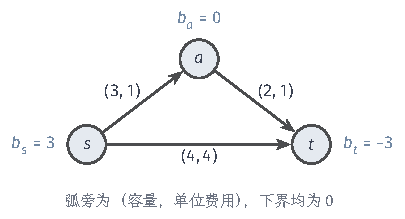
\includegraphics[width=68.527mm]{figures/01-basic-mathematics/04-graphs/tikz/c3-mcf-network/figure.pdf}
  \caption{三点最小费用流算例。$s$供给$3$单位，$t$需求$3$单位，$a$只做中转；弧旁括号依次为容量与单位费用，下界均为$0$。绕行$s\to a\to t$的单位费用为$2$，低于直达弧的$4$，但绕行量受$a\to t$的容量$2$限制。本节后面的计算都在这个网络上进行。}
  \label{fig:graph-opt-mcf-network}
\end{figure}

这个网络有许多可行流。$3$单位全走直达弧，费用为$3\times4=12$；让$2$单位绕行、$1$单位直达，费用为$2\times(1+1)+1\times4=8$。按弧序$s\to a$、$a\to t$、$s\to t$把流量写成向量，前者为$(0,0,3)$，后者为$(2,2,1)$。后面将证明$8$就是最小费用。

\paragraph{下界平移}
带正下界的弧在建模中很常见，例如合同规定某条线路至少运多少。处理办法是先把下界部分“预先送出”，再对剩余部分求解。令$x_{i,j}=\ell_{i,j}+y_{i,j}$，新变量满足$0\leq y_{i,j}\leq u_{i,j}-\ell_{i,j}$。预先送出的下界流量已经使顶点$i$净流出$\sum_j\ell_{i,j}-\sum_j\ell_{j,i}$，代入守恒式，$\bm y$应满足的剩余供需为
\[
  b'_i=b_i-\sum_{j:\,(i,j)\in E}\ell_{i,j}+\sum_{j:\,(j,i)\in E}\ell_{j,i}.
\]
目标变为$\sum c_{i,j}y_{i,j}+\bm c^{\top}\bm\ell$，后一项与$\bm y$无关。两个问题的可行解通过$\bm x=\bm\ell+\bm y$一一对应，费用处处相差同一个常数，所以最优解也一一对应。

图~\ref{fig:graph-opt-mcf-lower-bound}把三点网络中$s\to t$的下界改为$1$。平移后这条弧的容量从$4$变为$3$，同时$s$的剩余供给从$3$降为$2$，$t$的剩余需求从$3$降为$2$。如果只把容量减去下界而不修改供需，平移后的问题仍要求$s$送出$3$单位，下界那一单位就被重复计算了。新问题的最优解是$\bm y=(2,2,0)$，费用为$4$；加回常数$c_{s,t}\ell_{s,t}=4$，得到原问题的最优流$\bm x=(2,2,1)$与费用$8$。

\begin{figure}[!htb]
  \centering
  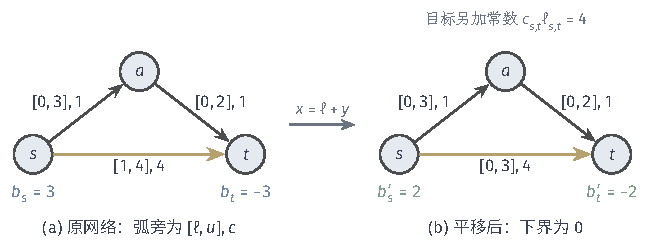
\includegraphics[width=109.767mm]{figures/01-basic-mathematics/04-graphs/tikz/c3-mcf-lower-bound-shift/figure.pdf}
  \caption{下界平移。(a)中黄色弧$s\to t$的流量须在$[1,4]$内，弧旁依次为流量区间与单位费用。(b)令$x=\ell+y$后，该弧的区间变为$[0,3]$，$s$与$t$的供需同时各减少$1$单位（绿色），目标另加常数$4$。容量和供需必须一起修改，只改其一会重复或遗漏下界那一单位。}
  \label{fig:graph-opt-mcf-lower-bound}
\end{figure}

上下界相等的弧流量已经固定，平移后容量为零，可以先删去，只保留它对供需和常数的贡献。还原时把平移量加回流量、把常数加回费用即可。以下除非特别说明，都假定下界已平移为零，固定弧已删去。

\paragraph{最优解的存在}
在有限上下界下，可行流集合由有限个线性等式与闭区间约束确定，是$\mathbb R^{a}$中的闭有界集，其中$a=|E|$。总费用是$\bm x$的线性函数，因而连续。由闭有界集上的极值定理~\ref{thm:multivariable-extreme-value}，只要可行流存在，最小费用一定能取到。可行流是否存在要另外判断，后文网络单纯形法的第一阶段就承担这一任务。

若允许某些弧的容量为无穷，可行集不再有界，最小值可能不存在。设可行流$\bm x$的残量网络（下一小节定义）中有一个负费用环，环上每条残量弧的剩余容量都是无穷，那么沿这个环可以推送任意多的流量，每推一单位都减少同样的正费用，总费用没有下界。本节主线只讨论有限容量。

还有一类常见问题：在源汇网络中先尽量多送，再在全部最大流中挑费用最低的，称为最小费用最大流。它分两步化成本节的问题：先用第~\ref{sec:graph-max-flow}节的方法求出最大流值$v^\star$，再令$b_s=v^\star$、$b_t=-v^\star$、其余$b_i=0$，求最小费用流。

\subsection{最优性条件}
\label{sec:graph-opt-mcf-optimality}

拿到一个可行流后，怎样判断它是否已经最便宜？逐一比较全部可行流行不通。第~\ref{sec:graph-max-flow}节判断最大流时，用残量网络把问题化成了“能否找到一条增广路径”。本小节沿用这一思路：先用残量网络描述所有保持供需的调整，再说明费用能否下降取决于其中是否有负费用环，最后借助节点势把环条件改写成逐弧可查的不等式。

\paragraph{残量网络与负费用环}
给定可行流$\bm x$。对每条原弧$(i,j)$，若$x_{i,j}<u_{i,j}$，建立正向残量弧$i\to j$，剩余容量为$u_{i,j}-x_{i,j}$，费用为$c_{i,j}$，表示再追加一单位要多付$c_{i,j}$；若$x_{i,j}>\ell_{i,j}$，建立反向残量弧$j\to i$，剩余容量为$x_{i,j}-\ell_{i,j}$，费用为$-c_{i,j}$，表示撤回一单位可以省下$c_{i,j}$。这与第~\ref{sec:graph-max-flow}节的残量网络相同，只是每条残量弧多带一个费用。原网络同时有$i\to j$与$j\to i$两条弧时，各自的残量弧要记住来自哪条原弧，不能合并成一个量。

沿残量网络中的有向环$C$推送$\theta>0$单位，是指对环上每条残量弧调整它的来源原弧：正向残量弧对应的原弧流量加$\theta$，反向残量弧对应的原弧流量减$\theta$。环上每个顶点恰有一条环弧进入、一条环弧离开，调整前后它的净流出不变，所以供需仍然满足；只要$\theta$不超过环上的最小剩余容量，上下界也仍然满足。总费用的改变量是$\theta\,c(C)$，其中$c(C)$是环上残量费用之和。于是，若$c(C)<0$，取正步长就能严格降低费用，当前流不是最优。

图~\ref{fig:graph-opt-mcf-residual-cycle}从全部走直达弧的可行流出发。残量网络中，$s\to a$与$a\to t$两条正向残量弧各费$1$，直达弧的反向残量弧$t\to s$费$-4$，三者构成费用为$1+1-4=-2$的环，剩余容量为$\min\{3,2,3\}=2$。沿这个环推送$2$单位，相当于把$2$单位从直达改为绕行，费用从$12$降为$12-2\times2=8$。

\begin{figure}[!htb]
  \centering
  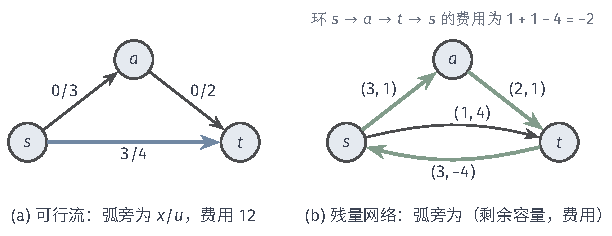
\includegraphics[width=103.579mm]{figures/01-basic-mathematics/04-graphs/tikz/c3-mcf-residual-cycle/figure.pdf}
  \caption{残量网络中的负费用环。(a)全部$3$单位走直达弧的可行流，弧旁为流量与容量。(b)它的残量网络，弧旁为剩余容量与费用；直达弧同时产生可追加$1$单位的正向残量弧和可撤回$3$单位、费用$-4$的反向残量弧$t\to s$。绿色环的费用为$-2$，沿它推送$2$单位使总费用降低$4$。}
  \label{fig:graph-opt-mcf-residual-cycle}
\end{figure}

\paragraph{环分解与最优性判据}
负费用环使费用可以下降。反过来，若残量网络中没有负费用环，是否就不存在更便宜的可行流？为此要说明：任何一个可行流与当前流之差，都能拆成残量网络中若干个环的叠加。

\begin{theorem}[负费用环判据]
\label{thm:graph-opt-negative-cycle}
可行流$\bm x$是最小费用流，当且仅当它的残量网络中不存在费用为负的有向环。
\end{theorem}

\begin{proof}
必要性已由上面的推送论证给出，下证充分性。任取可行流$\bm x'$，令$\bm d=\bm x'-\bm x$。两个流满足同一组供需，所以$\bm d$在每个顶点的净流出为零。逐条考察原弧$(i,j)$：若$d_{i,j}>0$，则$x_{i,j}<x'_{i,j}\leq u_{i,j}$，正向残量弧存在且剩余容量至少为$d_{i,j}$，在它上面放$d_{i,j}$；若$d_{i,j}<0$，则$x_{i,j}>x'_{i,j}\geq\ell_{i,j}$，反向残量弧存在，在它上面放$-d_{i,j}$。这样得到残量弧上的一组非负数$\bm g$，它在每个顶点的流入等于流出，并且按残量费用加权的总和等于$\sum_{(i,j)}c_{i,j}d_{i,j}=\bm c^{\top}\bm x'-\bm c^{\top}\bm x$。

接着把$\bm g$拆成环。若$\bm g\neq\bm 0$，从任一取正值的残量弧出发，沿正值弧前进：每到达一个顶点，它的流入为正，由流入等于流出，必有一条正值出弧可走。顶点只有有限个，前进中必然首次回到某个走过的顶点，由此截出一个有向环$C_1$。令$\lambda_1>0$为$\bm g$在$C_1$上的最小值，从环上各弧减去$\lambda_1$，剩余部分仍然非负且守恒，而取正值的弧至少少了一条。重复有限次，得到
\[
  \bm c^{\top}\bm x'-\bm c^{\top}\bm x=\sum_k\lambda_k\,c(C_k),\qquad\lambda_k>0.
\]
每个$C_k$都由残量弧组成。残量网络中没有负费用环时，右边每项非负，$\bm x'$不比$\bm x$便宜。
\end{proof}

判据回答的是怎样识别最优流，并不断言最优流唯一：若残量网络中有费用为零的环，沿它推送就得到另一个同费用的最优流。判据本身也不是完整的算法。反复寻找负费用环并沿它推送是一种自然的想法，但找哪个环、推多少、何时停止都要另行规定；下面的网络单纯形法给出一种具体的组织方式。

\paragraph{节点势与约化费用}
环判据要求检查所有的环，环的个数可能随图的规模指数增长。为了把它变成逐弧检查，给每个顶点$i$配一个实数$\pi_i$，称为\term{节点势}（node potential），并定义弧$(i,j)$的\term{约化费用}（reduced cost）
\begin{equation}
  \bar c_{i,j}=c_{i,j}-\pi_i+\pi_j.
  \label{eq:graph-opt-reduced-cost}
\end{equation}
残量弧使用同一公式：反向残量弧$j\to i$的费用为$-c_{i,j}$，约化费用为$-c_{i,j}-\pi_j+\pi_i=-\bar c_{i,j}$。

沿任一有向环把约化费用相加，每个顶点的势在离开它的弧上以$-\pi$出现一次、在进入它的弧上以$+\pi$出现一次，两两相消，所以环的约化费用之和等于原费用之和。因此，若能找到一组势，使所有残量弧的约化费用都非负，残量网络就没有负费用环。

反过来，残量网络没有负费用环时，这样的势一定存在。加入一个虚拟顶点$r$，从$r$向每个顶点连一条费用为零的弧。新弧都从$r$出发，没有弧进入$r$，所以新图的环都不经过$r$，仍然没有负环。由第~\ref{sec:graph-shortest-paths}节允许负边长的最短路结论，$r$到每个顶点$i$的最短距离$d_i$都是有限值（且$d_i\leq0$），并且对每条残量弧$i\to j$及其费用$c'$满足距离不等式$d_j\leq d_i+c'$。取$\pi_i=-d_i$，即得
\[
  c'-\pi_i+\pi_j=c'+d_i-d_j\geq0.
\]
所以“残量网络没有负费用环”与“存在使全部残量弧约化费用非负的势”等价，而后者只需逐弧检查。实际计算时可以用Bellman--Ford算法求$d_i$；若算法报告负环，就得到一个可以推送的负费用环。

\paragraph{逐弧最优性证书}
残量弧是否存在取决于原弧流量的位置，所以“全部残量弧的约化费用非负”可以翻译成原弧上的条件。弧$(i,j)$在下界时只有正向残量弧，要求$\bar c_{i,j}\geq0$；在上界时只有反向残量弧，要求$-\bar c_{i,j}\geq0$，即$\bar c_{i,j}\leq0$；严格位于两界之间时两条残量弧都存在，要求$\bar c_{i,j}=0$。下面的定理直接验证这组条件足以保证最优，不必再经过环分解。

\begin{theorem}[节点势最优性证书]
\label{thm:graph-opt-potential-certificate}
设固定弧已删去，$\bm x$是可行流，$\bm\pi$是一组节点势。若对每条弧$(i,j)$都有
\begin{equation}
  \bar c_{i,j}\ \begin{cases}
    \geq0, & x_{i,j}=\ell_{i,j},\\
    \leq0, & x_{i,j}=u_{i,j},\\
    =0, & \ell_{i,j}<x_{i,j}<u_{i,j},
  \end{cases}
  \label{eq:graph-opt-mcf-certificate}
\end{equation}
则$\bm x$是最小费用流。
\end{theorem}

\begin{proof}
任取可行流$\bm x'$。把$c_{i,j}=\bar c_{i,j}+\pi_i-\pi_j$代入费用差，
\[
  \bm c^{\top}(\bm x'-\bm x)=\sum_{(i,j)\in E}\bar c_{i,j}(x'_{i,j}-x_{i,j})+\sum_{(i,j)\in E}(\pi_i-\pi_j)(x'_{i,j}-x_{i,j}).
\]
第二个和按顶点重新归组，等于对每个$i$把$\pi_i$乘以顶点$i$在$\bm x'$与$\bm x$下净流出之差再求和；两个流满足同一组供需，这些差全为零。第一个和逐项非负：若$x_{i,j}=\ell_{i,j}$，则$x'_{i,j}-x_{i,j}\geq0$且$\bar c_{i,j}\geq0$；若$x_{i,j}=u_{i,j}$，则$x'_{i,j}-x_{i,j}\leq0$且$\bar c_{i,j}\leq0$；其余情形$\bar c_{i,j}=0$。所以$\bm c^{\top}\bm x'\geq\bm c^{\top}\bm x$。
\end{proof}

删去固定弧是为了避免$\ell_{i,j}=u_{i,j}$时前两个条件同时出现。条件~\eqref{eq:graph-opt-mcf-certificate}在线性规划中称为互补松弛条件，这里只用守恒式和每条弧允许的变化方向就完成了证明。流量$\bm x$与势$\bm\pi$合在一起构成一份证书：检查者核对可行性和每条弧上的一个符号，就能确认最优性，不必相信求解过程。回到三点网络，流$(2,2,1)$配上势$(\pi_s,\pi_a,\pi_t)=(4,3,0)$时，$s\to a$与$s\to t$都在两界之间，约化费用分别为$1-4+3=0$与$4-4+0=0$；$a\to t$在上界，约化费用为$1-3+0=-2\leq0$。三条弧都满足条件，所以费用$8$最小。

\subsection{网络单纯形法}
\label{sec:graph-opt-network-simplex}

定理~\ref{thm:graph-opt-potential-certificate}说明了停止时应该看到什么：一个可行流和一组势，逐弧满足符号条件。网络单纯形法始终保持流可行，并用一棵生成树确定势：树弧的约化费用被要求为零，由此解出势；再检查非树弧，若全部满足证书就停止，否则沿一个环改进流量。本小节以可行树基为算法状态，依次说明它的表示、第一个可行树基的构造、势的计算、环上的调整与状态更新，以及防止循环的选弧规则，最后用三点网络完整演示。

\paragraph{树基表示}
设下界已平移为零、固定弧已删去，并暂设底层无向图连通，即忽略弧的方向后连通。把弧集分成三部分：树弧集$T$，忽略方向后构成一棵生成树；取下界的非树弧集$L$；取上界的非树弧集$U$。三元组$(T,L,U)$称为一个\term{树基}（spanning tree basis）。非树弧的流量由它所在的集合直接给出，树弧的流量由守恒式决定。生成树总有叶子，叶子$v$只关联一条树弧，$v$的守恒式中其余各项（$b_v$与非树弧流量）都已知，于是解出这条树弧的流量；删去这个叶子及其树弧，把求出的流量计入相邻顶点的剩余供需，再对剩下的树重复，直到树弧全部求出。若求得的树弧流量都在上下界内，就称$(T,L,U)$为可行树基。

这里有两点容易误解。第一，树弧的流量允许恰好等于上界或下界；一条弧是否属于$T$取决于它在树中的位置，而不是流量是否严格在界内。第二，树不要求所有弧都朝向某个根，弧的方向只决定它在守恒式中取正号还是负号。

图~\ref{fig:graph-opt-ns-tree-basis}(a)是一个五点例子，供需为$b=(4,0,-2,1,-3)$，非树弧$1\to4$在上界、流量为$2$，$2\to5$在下界、流量为$0$。叶子$1$的守恒式为$x_{1,2}+x_{1,4}=4$，得$x_{1,2}=2$；叶子$4$的守恒式为$x_{4,3}-x_{1,4}=1$，得$x_{4,3}=3$，恰好等于这条树弧的容量；叶子$5$的守恒式为$-(x_{3,5}+x_{2,5})=-3$，得$x_{3,5}=3$。删去这三个叶子后，顶点$2$成为叶子，由$x_{2,3}+x_{2,5}-x_{1,2}=0$得$x_{2,3}=2$。最后剩下的顶点$3$的守恒式$x_{3,5}-x_{2,3}-x_{4,3}=3-2-3=-2$自动成立，因为全部供需之和为零。

\begin{figure*}[!htb]
  \centering
  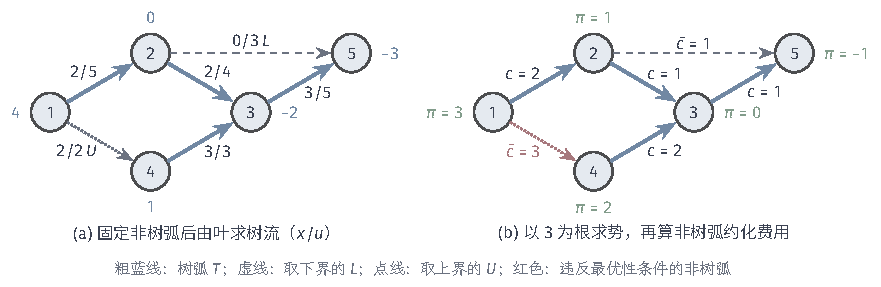
\includegraphics[width=149.144mm]{figures/01-basic-mathematics/04-graphs/tikz/c3-ns-tree-basis/figure.pdf}
  \caption{五点网络上的树基。粗蓝弧为树弧，虚线弧取下界，点线弧取上界。(a)顶点旁为供需量，弧旁为流量与容量；固定两条非树弧后，从叶子$1,4,5$开始逐个用守恒式求出树弧流量，树弧$4\to3$恰在上界仍属于树。(b)弧旁为单位费用或约化费用，绿色为以顶点$3$为根求出的节点势；树弧约化费用均为零，非树弧$1\to4$在上界却有$\bar c=3>0$（红色），违反最优性条件。}
  \label{fig:graph-opt-ns-tree-basis}
\end{figure*}

树流为什么由树唯一确定，可以用关联矩阵说明。按第~\ref{sec:graph-representations}节的约定，关联矩阵$\bm B\in\mathbb R^{n\times a}$中弧$(i,j)$对应的列在第$i$行为$1$、第$j$行为$-1$，守恒式就是$\bm B\bm x=\bm b$。$\bm B$各行之和为零，删去根所在的一行不丢失信息，记剩下的矩阵为$\tilde{\bm B}$。树弧对应的列组成$(n-1)$阶方阵$\tilde{\bm B}_T$。按上面消去叶子的次序排列行与列，每消去一个叶子，它所在的行在剩余树弧列中只有一个非零元，所以$\tilde{\bm B}_T$经行列重排后是三角矩阵，对角元为$\pm1$，从而可逆。于是$\bm x_T=\tilde{\bm B}_T^{-1}(\tilde{\bm b}-\tilde{\bm B}_N\bm x_N)$唯一确定，其中$N=L\cup U$；供需与界都是整数时，树流也是整数。

底层无向图不连通时，在消去固定弧后的各弱连通分量中分别处理：每个分量内的剩余供需之和必须为零，否则问题不可行；孤立顶点没有任何弧，它的供需必须为零。另外，同一个流量可能对应不同的树基，例如树弧恰在界上时，它也可能作为非树弧出现在另一个树基中。后面的退化现象正来自这种区别。

\paragraph{初始可行树基}
任意选一棵生成树、令非树弧取下界，求得的树流未必满足上下界。例如在三点网络中取$T=\{s\to a,a\to t\}$、$s\to t$取下界，叶子$a$与$t$迫使$x_{a,t}=3$，超过容量$2$。因此第一个可行树基要专门构造。

在下界已平移为零的网络中，先令全部原弧流量为零，再增加一个人工根$r$：每个$b_i>0$的顶点连人工弧$i\to r$，流量为$b_i$；每个$b_i<0$的顶点连人工弧$r\to i$，流量为$-b_i$；$b_i=0$的顶点连人工弧$i\to r$，流量为零。人工弧的容量取总供给$\sum_{b_i>0}b_i$，足以容纳这些流量。人工弧构成以$r$为中心的星形生成树，每个原顶点的守恒式都由它唯一的人工弧满足，于是得到一个显式的可行树基。

第一阶段令原弧费用为零、人工弧单位费用为一，目标就是人工流的总量，用下面介绍的同一套入弧、环调整与防循环操作求解。若第一阶段最优值为零，人工弧全部空载，原弧上的流量满足原问题的全部约束；若最优值为正，原问题没有可行流，因为原问题的任何可行流配上全零人工流都会使第一阶段目标为零。这一判定不依赖人为选定的“很大的费用常数”。

第一阶段结束后，删去人工根和全部人工弧。原来的树弧中去掉人工弧，留下一个森林；在原图的每个弱连通分量内，用连接不同森林分量的原非树弧把它补成生成树。补入的弧保持原流量不变，它们本来就在上界或下界，作为树弧恰在界上是允许的。随后恢复原费用、重新计算节点势，并从所得的可行树基重新设置防循环所需的数据，进入第二阶段。

\paragraph{节点势的计算}
给定树基，令根的势为零，沿树逐条解方程$c_{i,j}-\pi_i+\pi_j=0$，使每条树弧的约化费用为零。沿树弧方向从已知的$\pi_i$走到$j$时取$\pi_j=\pi_i-c_{i,j}$，逆着树弧方向从已知的$\pi_j$走到$i$时取$\pi_i=\pi_j+c_{i,j}$。换一个根只让全部势同加一个常数，约化费用不变。树流由供需与非树弧的界状态决定，势则只由树的结构与费用决定，两者分别计算。

图~\ref{fig:graph-opt-ns-tree-basis}(b)以顶点$3$为根：逆着$2\to3$得$\pi_2=0+1=1$，再逆着$1\to2$得$\pi_1=1+2=3$；逆着$4\to3$得$\pi_4=0+2=2$；顺着$3\to5$得$\pi_5=0-1=-1$。随后计算非树弧的约化费用：$2\to5$为$3-1+(-1)=1\geq0$，在下界，符合条件；$1\to4$为$4-3+2=3>0$，却在上界，违反条件。

树弧的约化费用都是零，无论流量位于何处都满足条件~\eqref{eq:graph-opt-mcf-certificate}。所以只要全部非树弧也满足条件，即$L$中的弧$\bar c\geq0$、$U$中的弧$\bar c\leq0$，当前流与势就构成最优性证书，算法停止。寻找违反条件的非树弧，称为定价。

\paragraph{入弧与环调整}
违反条件的非树弧有两类：$L$中$\bar c_{i,j}<0$的弧，应沿正向增加流量；$U$中$\bar c_{i,j}>0$的弧，应沿反向减少流量。选定这样一条入弧后，它与树上连接两端点的唯一路径构成一个环，称为\term{基本环}（fundamental cycle）。按入弧的调整方向给环定向：环上顺着定向经过的弧增加流量，逆着定向经过的弧减少流量。环上每个顶点一进一出，调整保持守恒。

推送一单位时，费用变化是环上各弧费用按增减取正负号之和。把每个$c$换成$\bar c+\pi_i-\pi_j$，势沿环相消，而树弧的约化费用为零，所以单位费用变化恰为入弧在调整方向上的约化费用：正向进入时为$\bar c_{i,j}<0$，反向进入时为$-\bar c_{i,j}<0$。

接着确定能推多远。对环上增加流量的弧计算$u-x$，对减少流量的弧计算$x-\ell$，入弧自身也参加比较，取最小值作为步长$\theta$。按$\theta$沿环更新后守恒仍然成立，上下界也都满足。$\theta>0$时费用严格下降$\theta|\bar c_{i,j}|$；$\theta=0$时流量不变，这种情形留到后面专门讨论。

\paragraph{出弧与状态更新}
达到步长$\theta$的弧称为阻塞弧，可能不止一条，按后述防循环规则从中选出一条。若选中的是树弧，它离开树，按它到达的是下界还是上界归入$L$或$U$，入弧则加入$T$。被删去的弧位于基本环上，删去后树仍然连通且无环，新的$T$仍是生成树。势需要更新：最简单的做法是沿新树从根重新计算一遍，便于逐步复核。更省的做法只调整一部分顶点：删去出弧后树分成两块，只有不含根的那一块的势改变，且同加或同减入弧的约化费用。

若选中的是入弧自身，说明它先到达了另一端的界，便从$L$转入$U$或从$U$转入$L$，树和势都不变。这种\emph{界翻转}同样是合法的一次迭代，所以不能把每一轮都描述为两条不同的弧互相交换。

\begin{algorithm}[网络单纯形法]
\label{alg:graph-opt-network-simplex}
输入：有限有向网络，供需$b_i$，有限上下界与单位费用。输出：最优流$\bm x$、费用与节点势$\bm\pi$，或“不可行”的结论。状态：树基$(T,L,U)$、各弧流量（含扰动系数）、树的父顶点与深度、节点势。
\begin{enumerate}
  \item 平移下界、删去固定弧；在每个弱连通分量内检查供需之和为零。
  \item 第一阶段：增加人工根与人工弧，取星形可行树基，原弧费用为零、人工弧费用为一，并按当前树基设置防循环数据。
  \item 计算节点势与非树弧的约化费用；若没有违反条件的非树弧，转第6步。
  \item 选一条违反条件的入弧，构造基本环，比较环上各弧（含入弧）的剩余量得到步长$\theta$，按防循环规则选出阻塞弧。
  \item 沿环更新流量；若出弧是树弧，作树弧交换，否则作界翻转。回到第3步。
  \item 第一阶段停止时，若人工流总量为正，报告不可行；否则删去人工结构，补成原网络的可行树基，恢复原费用并重新设置防循环数据，以第二阶段身份回到第3步。第二阶段停止时，还原下界平移，返回流量、费用与节点势。
\end{enumerate}
\end{algorithm}

\paragraph{退化与防循环}
步长为零的迭代称为\term{退化换基}（degenerate pivot）。它发生在基本环上某条弧已经处在阻塞方向的界上时，通常就是恰在界上的树弧。图~\ref{fig:graph-opt-ns-degenerate}把三点网络中$s\to t$的容量改为$1$，从$T=\{s\to a,a\to t\}$、$U=\{s\to t\}$出发，流量为$(2,2,1)$，树弧$a\to t$已在上界。势为$(2,1,0)$，$s\to t$在上界而$\bar c_{s,t}=4-2+0=2>0$，应反向进入；基本环上$a\to t$要增加流量，剩余量为$0$，所以$\theta=0$。$a\to t$出基进入$U$，$s\to t$进入树，流量和费用都没变，树基却变了。在新树基下势为$(4,3,0)$，$\bar c_{a,t}=-2\leq0$，满足条件，算法停止。

\begin{figure}[!htb]
  \centering
  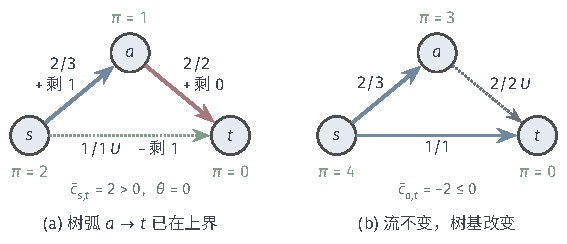
\includegraphics[width=96.054mm]{figures/01-basic-mathematics/04-graphs/tikz/c3-ns-degenerate/figure.pdf}
  \caption{退化换基。三点网络中$s\to t$的容量改为$1$，弧旁为流量与容量，“剩”为沿基本环调整方向的剩余量，绿色$\pi$为节点势。(a)入弧$s\to t$（绿色）在上界且约化费用为正，反向进入；树弧$a\to t$（红色）已在上界，剩余量为零，步长为零。(b)$a\to t$出基后流量与费用不变，新树基的势使全部非树弧满足最优性条件。}
  \label{fig:graph-opt-ns-degenerate}
\end{figure}

这个例子中的退化换基换来了一份最优性证书，但一般情形下，连续的零步长换基可能在若干个树基之间兜圈子，回到已经出现过的树基，费用始终不变，算法不再前进。因此，“费用不增加”本身不足以保证有限终止，阻塞弧有多条时选哪一条，必须写进算法。只取编号最小的弧不能排除循环，需要专门构造的规则。下面说明适用于有上下界弧的\term{词典序规则}（lexicographic rule）。

把上界写成等式$x_{i,j}+s_{i,j}=u_{i,j}$，$s_{i,j}\geq0$是上界松弛量。这样，每条弧有两个离界距离：$x_{i,j}-\ell_{i,j}$与$s_{i,j}$。非退化的情形是每条树弧的两个离界距离都为正，步长才一定为正。词典序规则用一个符号扰动人为地制造这种情形。在一个阶段开始时，把当前可行树基的树弧编号为$e_1,\ldots,e_{n-1}$，把$e_k$的流量改为$x_{e_k}+\sigma_k\varepsilon^k$：若$e_k$在上界取$\sigma_k=-1$，否则取$\sigma_k=+1$。供需随之改为扰动后流量所对应的净流出，并在整个阶段内保持不变；非树弧仍恰在界上。这里$\varepsilon$看作充分小的正数，每个量都表示成$(\text{常数},\varepsilon\text{的系数},\ldots,\varepsilon^{n-1}\text{的系数})$这样的向量，比较大小就是从常数项起按分量逐个比较，即词典序比较。于是每条树弧的两个离界距离在词典序下都严格为正。

每轮比较步长时，增加流量的树弧以向量$u-x(\varepsilon)$为候选，减少流量的树弧以$x(\varepsilon)-\ell$为候选，入弧以$(u-\ell,0,\ldots,0)$为候选，取词典序最小者作为步长$\theta(\varepsilon)$并让它出基。初始时各树弧的$\varepsilon$系数行是$\pm$单位向量，线性无关；每次换基，留下的树弧系数行加减出弧的系数行，入弧取出弧系数行的正负，这是可逆的行变换，界翻转则不改变系数行。所以各树弧的系数行始终线性无关，两条树弧的候选向量不会相等，入弧的候选向量与任一树弧也不会相等，词典序最小者唯一。更新后出弧恰好落在界上，其余树弧仍严格在界内，扰动后的问题始终非退化。

还原到基本环上，这个规则只在实际步长出现并列时起作用：比较并列阻塞弧的$\varepsilon$系数，选词典序最小的那条出基，实际流量仍按常数项更新。它为什么能防止循环，在下一小节的分析中说明。两个阶段各自从初始可行树基设置扰动：第一阶段从星形树基开始，第二阶段从清理人工结构后得到的树基重新开始。另一类常用规则要求维护所谓强可行树，它有自己的方向约定与初始化要求；第一阶段清理只保证得到普通的可行树基，不能据此断言原网络已经具有强可行树，这里不展开。

\paragraph{迭代算例}
回到图~\ref{fig:graph-opt-mcf-network}的三点网络，先做第一阶段。人工弧容量取总供给$3$，星形初始树为$s\to r$、$r\to t$、$a\to r$，流量依次为$3,3,0$，人工流总量为$6$，见图~\ref{fig:graph-opt-ns-artificial-start}(a)。按这个次序设置扰动，前两条树弧在上界，扰动后的流量为$3-\varepsilon$与$3-\varepsilon^2$，$a\to r$为$\varepsilon^3$。以$r$为根，第一阶段费用下的势为$(\pi_s,\pi_a,\pi_t,\pi_r)=(1,1,-1,0)$，非树弧$s\to t$与$a\to t$的约化费用都是$-2$。

\begin{figure*}[!htb]
  \centering
  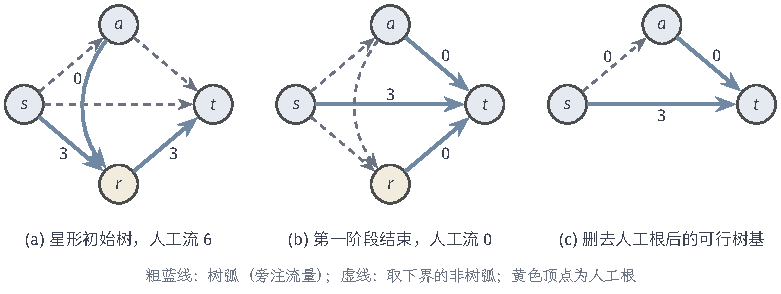
\includegraphics[width=132.186mm]{figures/01-basic-mathematics/04-graphs/tikz/c3-ns-artificial-start/figure.pdf}
  \caption{两阶段法的第一阶段。(a)增加人工根$r$（黄色），供给点、需求点和中转点分别用人工弧连向或连自$r$，得到显式可行的星形树，人工流总量为$6$。(b)两次换基后人工流降为零，原弧$s\to t$承担全部$3$单位，空载的人工弧$r\to t$仍在树中。(c)删去人工根和人工弧，剩下的树弧恰好构成原网络的生成树，作为第二阶段的初始可行树基。}
  \label{fig:graph-opt-ns-artificial-start}
\end{figure*}

选$s\to t$入弧。基本环上$s\to t$增加，$r\to t$与$s\to r$减少，剩余量依次为$4$、$3$、$3$，实际步长并列。两条并列弧的候选向量为$(3,0,-1,0)$与$(3,-1,0,0)$，后者词典序更小，所以$s\to r$出基。更新后$s\to t$承担$3$单位，人工流的常数部分已经为零。新势为$(-1,1,-1,0)$，$a\to t$的约化费用为$0-1+(-1)=-2$，再次入弧；这次$r\to t$与$a\to r$的剩余量都是$0$，是一次退化换基，比较$\varepsilon$系数后$a\to r$出基。此时全部非树弧满足条件，第一阶段最优值为零，见图~\ref{fig:graph-opt-ns-artificial-start}(b)。删去$r$后，树弧$s\to t$与$a\to t$已经构成原网络的生成树，$s\to a$在下界，这就是第二阶段的初始树基。

第二阶段从$T=\{s\to t,a\to t\}$、流量$(0,0,3)$开始，总费用为$12$。以$t$为根，逆着$s\to t$得$\pi_s=4$，逆着$a\to t$得$\pi_a=1$，势为$(4,1,0)$。非树弧$s\to a$在下界，约化费用为$1-4+1=-2<0$，选它正向入弧。基本环为$s\to a\to t$再逆着$s\to t$回到$s$：$s\to a$与$a\to t$增加，剩余量为$3$与$2$；$s\to t$减少，剩余量为$3$。步长$\theta=2$，由$a\to t$达到，费用下降$2\times2=4$。

$a\to t$到达上界，出基进入$U$，$s\to a$进入树。新流量为$(2,2,1)$，总费用为$8$。以$t$为根重新计算，$\pi_s=4$，顺着$s\to a$得$\pi_a=4-1=3$，势为$(4,3,0)$。唯一的非树弧$a\to t$在上界，约化费用为$1-3+0=-2\leq0$，满足条件，算法停止。这正是上一小节核对过的最优性证书。

再把$s\to a$的容量改为$1$，从同一初始树基出发。势与约化费用都不变，$s\to a$仍正向入弧，但三条弧的剩余量变为$1$、$2$、$3$，步长为$1$，由入弧自身达到。于是作界翻转：$s\to a$从$L$转入$U$，树不变，流量为$(1,1,2)$，费用为$10$。势仍为$(4,1,0)$，$s\to a$在上界，约化费用$-2\leq0$；没有其他非树弧，算法停止。逐项核对：$s$的净流出$1+2=3$，$a$的净流出$1-1=0$，$t$的净流出$-1-2=-3$，各弧流量都在界内。

图~\ref{fig:graph-opt-ns-pivots}把两种情形并排比较。两者从同一个树基、同一条入弧出发，只因入弧容量不同，阻塞弧一次是树弧、一次是入弧自身，分别对应树弧交换与界翻转。

\begin{figure*}[!htb]
  \centering
  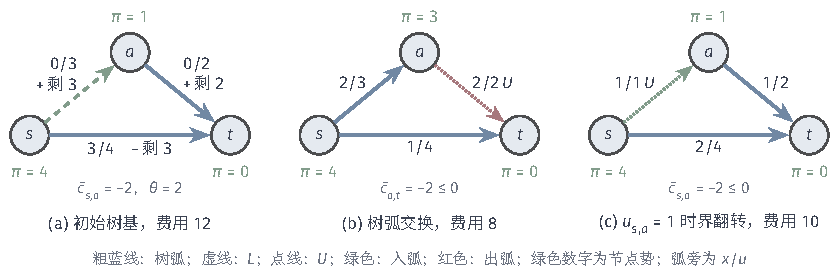
\includegraphics[width=142.053mm]{figures/01-basic-mathematics/04-graphs/tikz/c3-ns-pivots/figure.pdf}
  \caption{第二阶段的两种迭代。弧旁为流量与容量，“$+$剩”“$-$剩”为沿基本环增加或减少流量时的剩余量，$\pi$为节点势。(a)初始树基中$s\to a$的约化费用为$-2$，沿基本环最多推送$2$单位。(b)阻塞弧是树弧$a\to t$，它出基进入$U$，费用由$12$降为$8$。(c)若$s\to a$容量为$1$，入弧自身先到上界，树不变，费用降为$10$。两种结局中非树弧的约化费用都满足符号条件。}
  \label{fig:graph-opt-ns-pivots}
\end{figure*}

\subsection{算法分析与结果检验}
\label{sec:graph-opt-ns-analysis}

前面逐步说明了网络单纯形法的各个操作，本小节把它们合起来，回答三个问题：每轮迭代是否保持可行并改进费用，算法是否一定停止，停止时得到的是什么、要花多少计算。

\paragraph{可行性与费用变化}
每轮迭代沿基本环调整流量，环上每个顶点一进一出，各顶点的净流出不变；步长取环上各弧剩余量的最小值，所以调整后上下界仍然满足。树弧交换后新的$T$仍是生成树，出弧落在它所到达的界上，被正确归入$L$或$U$；界翻转只改变入弧的界状态。因此，每轮结束时都得到一个可行树基。费用的变化等于步长乘以入弧在调整方向上的约化费用，后者为负：步长为正时费用严格下降，步长为零时费用不变而树基改变。

\paragraph{有限终止}
仅凭费用不增不能推出有限终止，因为零步长的换基可能循环。词典序规则补上了这一缺口。在一个阶段内，扰动后的供需固定不变，扰动后的流量由树基$(T,L,U)$唯一确定，所以扰动后的费用（一个关于$\varepsilon$的多项式）是树基的函数。扰动后的问题非退化，每轮的步长$\theta(\varepsilon)$在词典序下严格为正，扰动后的费用便在词典序下严格下降，已经出现过的树基不可能再出现。可能的树基只有有限个：$T$是有限多棵生成树之一，每条非树弧只有两种界状态。所以每个阶段都在有限轮后停止。

停止时全部非树弧满足符号条件，树弧约化费用为零，由定理~\ref{thm:graph-opt-potential-certificate}，当前流在本阶段的费用下最优。对第一阶段，这给出可行性的判定；对第二阶段，这给出原问题的最优流。以上论证都假设精确运算。

\paragraph{单轮开销}
设顶点数为$n$，弧数为$a$。朴素实现每轮扫描全部非树弧计算约化费用，需要$O(a)$次运算；为树记录父顶点与深度后，从入弧两端沿父指针上溯到最近公共祖先即可找出基本环，并沿环比较剩余量、更新流量，都是$O(n)$；沿新树重新计算势也是$O(n)$。所以每轮为$O(n+a)$次运算，只扫描部分弧的定价策略可以降低这一项。总开销还取决于迭代轮数，其中包括退化换基。上面的有限性论证只给出与树基个数相当的上界，不能从每轮简单推出总运算量具有统一的多项式界；本书也不据此断言网络单纯形法一定快于专门的最大流或指派算法。

\paragraph{结果检验}
输出须回到原始问题检查：先把下界平移量加回流量，核对每个顶点的净流出等于原始$b_i$、每条弧满足原始上下界，再按原始费用重算目标值，并确认它等于平移后问题的费用加上常数$\bm c^{\top}\bm\ell$。最优性则逐弧核对势条件~\eqref{eq:graph-opt-mcf-certificate}。浮点实现中，守恒误差、界约束误差与约化费用的符号都只能在容差内判断，应分别报告；近似满足的条件说明结果接近最优，不能直接当作精确证书。

\paragraph{与其他问题的关系}
最大流与最小费用流使用同一种残量网络，但改进方式不同：最大流沿源汇之间的增广路径增加输送量，最小费用流在供需固定时沿环调整流量以减少费用。下一节的匹配可以写成单位容量的最大流，第~\ref{sec:graph-assignment}节的指派则可以写成单位容量的最小费用流。尽管如此，后面两节仍分别介绍专门的增广算法：一般模型说明问题之间可以互相转写，专门算法则利用二部配对的结构，状态更简单，开销也有更直接的界。

% 第3章第5节：匹配（二部图匹配问题；交替路径、单位容量网络与最优性条件；增广匹配算法；算法分析与结果检验）。

\section{匹配}
\label{sec:graph-matching}

把若干任务分给若干名人员，每人至多接一项任务，每项任务至多由一人完成，而且只有具备相应资格的人才能接某项任务。目标是让完成配对的任务尽可能多。这里选择的对象是一组“人员—任务”配对，约束是任何人员或任务都不能出现在两个配对中。

本节先给出二部图匹配的定义，并用小例子区分“无法直接再加边”与“边数最多”。随后以交替路径建立改进机制：沿一条两端都未配对的交替路径翻转选边状态，配对数就增加一；借助单位容量的流网络，第~\ref{sec:graph-max-flow}节的最大流判据给出相应的最大性条件。最后把这一机制写成增广匹配算法，分析开销并说明怎样验收结果。本节只比较配对的数量，不涉及配对的成本。

\subsection{二部图匹配问题}
\label{sec:graph-opt-match-problem}

人员与任务分属两类对象，资格关系只连接一名人员与一项任务，同类对象之间没有边。若无向图的顶点集能分成两个不相交的部分$U$与$W$，使每条边都恰有一个端点在$U$、另一个端点在$W$，就称它为\term{二部图}（bipartite graph），记作$\mathcal G=(U\cup W,E)$。本节称$U$为左侧、$W$为右侧，两侧的顶点数可以不同。

\begin{definition}[匹配]
\label{def:graph-opt-matching}
图$\mathcal G=(V,E)$中两两没有公共端点的边组成的集合$M\subseteq E$称为一个\term{匹配}（matching）。$M$中某条边的端点称为被$M$饱和，其余顶点称为自由顶点。饱和全部顶点的匹配称为\term{完美匹配}（perfect matching）。不能再加入任何一条边而仍为匹配的$M$称为\term{极大匹配}（maximal matching），边数最多的匹配称为\term{最大匹配}（maximum matching）。
\end{definition}

最大匹配一定是极大匹配，反过来不成立。图~\ref{fig:graph-opt-match-maximal-maximum}中允许边为$a-x$、$a-y$、$b-x$。若先选了$a-x$，$a$与$x$都已被占用，剩下的两条边各与它共享一个端点，无法再加，所以$\{a-x\}$是极大匹配；但$\{a-y,b-x\}$有两条边，是最大匹配，也是完美匹配。从$\{a-x\}$到$\{a-y,b-x\}$，靠的不是继续加边，而是把$a$的配对从$x$改到$y$，腾出$x$给$b$。这说明逐条贪心加边可能停在较差的结果上，重排已有配对才是改进的关键。

\begin{figure}[!htb]
  \centering
  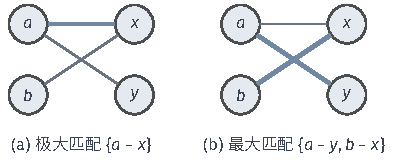
\includegraphics[width=67.07mm]{figures/01-basic-mathematics/04-graphs/tikz/c3-match-maximal-maximum/figure.pdf}
  \caption{极大匹配与最大匹配。细线为允许的配对，粗蓝线为选中的匹配边。(a)$\{a-x\}$已无法再加入任何边，是极大匹配；(b)$\{a-y,b-x\}$的边数更多，是最大匹配。由(a)到(b)须改动已有的配对$a-x$。}
  \label{fig:graph-opt-match-maximal-maximum}
\end{figure}

本节的目标只是最大化$|M|$，边上没有费用；要求完成配对并比较成本的问题留到第~\ref{sec:graph-assignment}节。两侧大小不同时，最大匹配至多有$\min\{|U|,|W|\}$条边，但未必达到这个数：若左侧两个顶点都只与右侧同一个顶点相连，无论怎样选，至多只有一个能配上。下面的构造还依赖两侧的划分。一般的无向图可能含有奇数长的环，例如三角形，它的顶点无法分成两侧使每条边跨侧，下面的单位容量网络构造对它不适用，一般图的匹配需要另外的机制。

\subsection{交替路径与最优性条件}
\label{sec:graph-opt-match-alternating}

图~\ref{fig:graph-opt-match-maximal-maximum}中的改进可以这样描述：从自由顶点$b$出发，先走未选的边$b-x$，再走已选的边$x-a$，最后走未选的边$a-y$到达自由顶点$y$，然后把这条路径上每条边的选中状态取反。下面把这一操作一般化。

给定匹配$M$，若一条路径上的边交替地不属于$M$与属于$M$，称它为\term{交替路径}（alternating path）。两个端点都是自由顶点的交替路径称为关于$M$的增广路径。增广路径的首尾两条边都不在$M$中，因为端点自由；所以路径上不在$M$中的边比在$M$中的边恰好多一条。

\begin{lemma}[沿增广路径翻转]
\label{lem:graph-opt-match-flip}
设$P$是关于匹配$M$的增广路径，把$P$上属于$M$的边移出、不属于$M$的边加入，得到的边集$M'$仍是匹配，且$|M'|=|M|+1$。
\end{lemma}

\begin{proof}
不在$P$上的顶点所关联的选边没有变化。$P$的内部顶点在翻转前恰关联$P$上的一条匹配边和一条非匹配边，翻转后两者互换，仍恰关联一条选边；它不会关联$P$以外的匹配边，因为它在$M$中的唯一配对已经在$P$上。$P$的两个端点原来是自由的，翻转后各关联一条选边。所以$M'$中没有两条边共享端点。由于$P$上非匹配边比匹配边多一条，$|M'|=|M|+1$。
\end{proof}

\paragraph{单位容量网络}
增广路径与第~\ref{sec:graph-max-flow}节的增广路径同名，并非巧合。由二部图构造流网络：增加源点$s$与汇点$t$，从$s$向每个$u\in U$连容量为$1$的弧，每条允许边$u-w$改为容量为$1$的弧$u\to w$，再从每个$w\in W$向$t$连容量为$1$的弧。图~\ref{fig:graph-opt-match-flow-network}画出了一个这样的网络。

给定匹配$M$，在每条匹配边$u-w$对应的路线$s\to u\to w\to t$上各送一单位，得到流值为$|M|$的整数流。反过来，设$\bm x$是一个整数流，每条弧的流量只能是$0$或$1$。顶点$u\in U$只有一条容量为$1$的入弧，流守恒使它至多有一条流量为$1$的出弧；同理，每个$w\in W$至多有一条流量为$1$的入弧。所以流量为$1$的中间弧对应的边两两不共享端点，构成一个匹配，边数等于流值。整数流与匹配就这样一一对应，并且流值等于边数。不能用分数流量四舍五入来代替这一对应：分数流不直接给出配对。

在这个对应下，残量网络中的$s$到$t$简单路径恰好是增广路径。设$\bm x$对应匹配$M$。从$s$出发，正向残量弧$s\to u$存在当且仅当$u$自由；从左侧顶点$u$，可以沿正向残量弧走到任一个与$u$由非匹配边相连的$w$；从右侧顶点$w$，若$w$自由可以走$w\to t$到达汇点，否则只能沿反向残量弧$w\to u'$回到它的配对$u'$，相当于准备撤回匹配边$u'-w$。所以这样一条路径依次经过一个自由左侧顶点、交替的非匹配边与匹配边、一个自由右侧顶点，沿它增广恰好就是引理~\ref{lem:graph-opt-match-flip}中的翻转。

\begin{figure}[!htb]
  \centering
  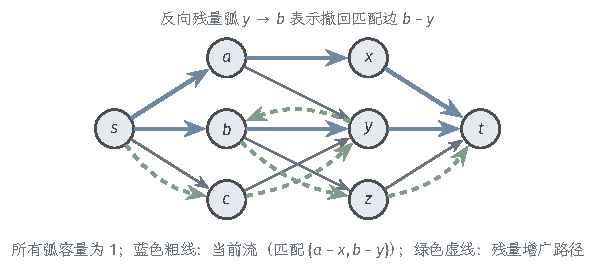
\includegraphics[width=100.76mm]{figures/01-basic-mathematics/04-graphs/tikz/c3-match-flow-network/figure.pdf}
  \caption{二部图匹配的单位容量网络。允许边为$a-x,a-y,b-y,b-z,c-y$，全部弧容量为$1$。蓝色粗弧是匹配$\{a-x,b-y\}$对应的流，流值为$2$。绿色虚线是残量网络中的一条$s$到$t$路径，其中$y\to b$是反向残量弧，表示撤回匹配边$b-y$；这条路径对应交替路径$c-y-b-z$。}
  \label{fig:graph-opt-match-flow-network}
\end{figure}

\paragraph{最大性条件}
有了上面的对应，最大流的判据可以直接搬到匹配上。

\begin{theorem}[增广路径判据]
\label{thm:graph-opt-match-augmenting}
二部图中的匹配$M$是最大匹配，当且仅当不存在关于$M$的增广路径。
\end{theorem}

\begin{proof}
若存在增广路径，由引理~\ref{lem:graph-opt-match-flip}可得更大的匹配，$M$不是最大的。反过来，设不存在增广路径，令$\bm x$是$M$对应的流。由上面的对应，$\bm x$的残量网络中没有$s$到$t$的路径，由第~\ref{sec:graph-max-flow}节的增广路径判据，$\bm x$是最大流。任何匹配$M''$对应一个流值为$|M''|$的流，所以$|M''|\leq\operatorname{val}(\bm x)=|M|$，$M$是最大匹配。
\end{proof}

整数容量时Ford--Fulkerson方法输出整数最大流，所以最大流值总能由某个匹配达到，最大流值就等于最大匹配的边数。

判据与“不能再加一条边”的区别，可以在图~\ref{fig:graph-opt-match-augment}上看清。允许边为$a-x$、$a-y$、$b-y$、$b-z$、$c-y$，当前匹配为$\{a-x,b-y\}$。剩下的三条边$a-y$、$b-z$、$c-y$都与已选边共享端点，所以这个匹配是极大的。但从自由顶点$c$出发，走非匹配边$c-y$、匹配边$y-b$、非匹配边$b-z$，到达自由顶点$z$，得到增广路径$c-y-b-z$。翻转后撤去$b-y$，加入$c-y$与$b-z$，匹配变为$\{a-x,b-z,c-y\}$，大小由$2$增为$3$。

\begin{figure*}[!htb]
  \centering
  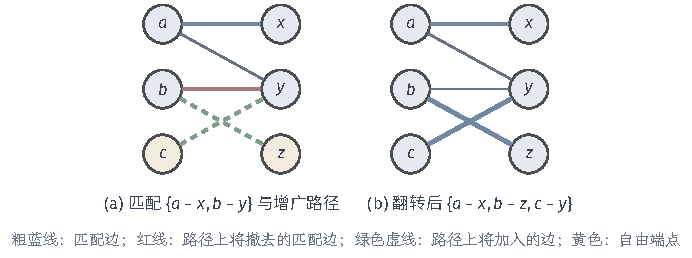
\includegraphics[width=117.094mm]{figures/01-basic-mathematics/04-graphs/tikz/c3-match-augment/figure.pdf}
  \caption{沿交替路径翻转。(a)匹配$\{a-x,b-y\}$是极大匹配，但自由顶点$c$与$z$（黄色）之间有增广路径$c-y-b-z$：绿色虚线为路径上将加入的非匹配边，红线为将撤去的匹配边。(b)翻转后$a-x$保留，$b-y$被$b-z$与$c-y$取代，配对数增加一。}
  \label{fig:graph-opt-match-augment}
\end{figure*}

\subsection{增广匹配算法}
\label{sec:graph-opt-match-algorithm}

定理~\ref{thm:graph-opt-match-augmenting}给出一个算法：只要存在增广路径就沿它翻转，不存在时停止。剩下的问题是怎样在二部图上直接搜索增广路径，而不必显式建立流网络。

算法维护的状态包括：两侧每个顶点的配对伙伴（自由顶点记为空），以及每轮搜索使用的访问标记和右侧顶点的前驱。每轮搜索同时从所有自由左侧顶点出发，用一个队列作广度优先遍历。从左侧顶点$u$出发时，检查它的每个邻居$w$：若$w$尚未访问，则标记$w$并记前驱为$u$；这时若$w$自由，就找到了增广路径，否则把$w$的配对伙伴放入队列，相当于沿匹配边从$w$回到左侧。队列耗尽仍未到达自由右侧顶点，说明当前不存在增广路径。这一搜索恰好就是在单位容量网络的残量网络中从$s$出发的遍历，只是省去了$s$与$t$。

找到自由右侧顶点$w$后，沿前驱回溯：$w$的前驱是左侧顶点$u$，若$u$不自由，再从$u$的原配对伙伴继续回溯，直到到达作为出发点的自由左侧顶点。回溯得到的就是一条增广路径，沿它统一翻转配对伙伴。搜索过程中匹配保持不变，只有完整找到增广路径之后才修改，这样前驱链始终描述同一个匹配下的交替路径。

\begin{algorithm}[增广匹配]
\label{alg:graph-opt-augmenting-matching}
输入：二部图$\mathcal G=(U\cup W,E)$的邻接表。输出：最大匹配$M$，以及最后一次失败搜索的已访问顶点集。状态：两侧顶点的配对伙伴、访问标记、右侧顶点的前驱、队列。
\begin{enumerate}
  \item 令$M=\varnothing$，全部配对伙伴为空。
  \item 清除访问标记，把所有自由左侧顶点放入队列并标记。
  \item 逐个取出左侧顶点$u$，对每个未访问的邻居$w$作标记并令其前驱为$u$；若$w$自由，转第4步，否则把$w$的配对伙伴标记后放入队列。队列耗尽时转第5步。
  \item 从$w$沿前驱与原配对伙伴交替回溯到一个自由左侧顶点，沿这条增广路径翻转配对伙伴，回到第2步。
  \item 输出$M$与本轮的已访问顶点集，停止。
\end{enumerate}
\end{algorithm}

\paragraph{算例}
在图~\ref{fig:graph-opt-match-augment}的二部图上，从$M=\{a-x,b-y\}$开始。自由左侧顶点只有$c$。从$c$检查邻居$y$，记前驱$y\leftarrow c$；$y$已与$b$配对，把$b$放入队列。从$b$检查邻居：$y$已访问，$z$未访问，记前驱$z\leftarrow b$，而$z$自由，找到增广路径。回溯：$z$的前驱是$b$，$b$原来配$y$，$y$的前驱是$c$，$c$自由，路径为$c-y-b-z$。翻转后$c$配$y$，$b$配$z$，$a$仍配$x$，得到大小为$3$的匹配。

下一轮开始时已没有自由左侧顶点，队列一开始就是空的，搜索立即失败，算法停止。这时$|M|=3=|U|$，结论也可以直接从上界看出。若把边$b-z$删去，情形就不同了：从$c$到$y$，再沿匹配边到$b$，$b$的邻居只有已访问的$y$，队列耗尽，不存在增广路径，匹配$\{a-x,b-y\}$就是最大匹配。这里虽然仍有自由顶点$c$与$z$，但不存在连接它们的交替路径，所以不能再改进。对应的残量网络中，从$s$可达的顶点集为$\{s,c,y,b\}$，跨出这一集合的弧是满流的$s\to a$与$y\to t$，割容量为$2$，等于匹配的边数。

\subsection{算法分析与结果检验}
\label{sec:graph-opt-match-analysis}

\paragraph{计算开销}
记$n=|U|+|W|$，$m$为允许边数，$\nu=\min\{|U|,|W|\}$。每次成功的翻转使匹配增加一条边，而匹配至多有$\nu$条边，所以成功的搜索不超过$\nu$次，再加上最后一次失败的搜索。一轮搜索中每个顶点至多入队或标记一次，每条边至多从它的左端点检查一次，所以搜索为$O(n+m)$；回溯与翻转沿一条路径进行，为$O(n)$；初始化配对数组为$O(n)$。总运算量为$O(\nu(n+m))$。还有按层同时寻找多条增广路径的更快的匹配算法，本书不展开，也不引用它们的复杂度界。

\paragraph{结果检验}
检验分两步。可行性：逐条核对所选边都是允许边、任意两条所选边没有公共端点，再重新数出边数。最大性：可以重做一次从全部自由左侧顶点出发的交替搜索，确认到达不了自由右侧顶点；也可以用最后一次失败搜索的已访问顶点集加上$s$构造单位容量网络中的割，核对割容量等于匹配边数，这是一份不依赖算法过程的证书。不能因为每个自由左侧顶点都不与自由右侧顶点直接相连就宣布最大，图~\ref{fig:graph-opt-match-augment}(a)正是这种情形，而那里仍有增广路径。

% 第3章第6节：指派（指派问题与模型变形；可行标号与紧边证书；匈牙利算法；算法分析、结果检验与问题比较）。

\section{指派}
\label{sec:graph-assignment}

上一节只关心能配上多少对。现在每个对象都必须完成配对，而不同配对的成本不同：把$N$项工作分给$N$名工人，每人做一项，工人$i$做工作$j$的耗时为$c_{i,j}$，要使总耗时最少。可行解仍是二部图中的匹配，而且必须是完美匹配；新增的是边上的成本，以及证明一个解已经最省的手段。

本节先写出指派问题及几种常见变形。随后给行与列配置标号，用它们给出任何完整指派成本的下界，并说明只用“紧边”完成的指派恰好达到这个下界。匈牙利算法同时维护可行标号与由紧边组成的匹配：匹配用上一节的交替路径扩大，扩大不了时调整标号以产生新的紧边。最后分析开销，说明怎样检验结果，并比较最大匹配、指派与最小费用流三种问题。

\subsection{指派问题}
\label{sec:graph-opt-assign-problem}

把工人看成左侧的行，工作看成右侧的列。行$i$与列$j$之间允许配对时，配对成本$c_{i,j}$是有限实数；不允许的配对没有边。

\begin{definition}[指派问题]
\label{def:graph-opt-assignment}
设有$N$行、$N$列，允许的行列对组成边集$E$，每条边$(i,j)\in E$有有限实成本$c_{i,j}$。\term{指派问题}（assignment problem）要求选出一个完美匹配，即给每行指定一个不同的列，并且只用允许边，使总成本$\sum_i c_{i,\sigma(i)}$最小，其中$\sigma(i)$是分给行$i$的列。
\end{definition}

全部行列对都允许时，$\sigma$可以是任意置换，用$0$-$1$变量$x_{i,j}$表示就是每行每列恰选一个元素。行数少于列数的矩形情形，可以补充若干虚拟行，它们到每一列的成本都是零：补成方阵后，虚拟行只占用原来没有被真实行使用的列，总成本不变，删去虚拟行的配对就得到原问题的解。

实际问题中还要分清三种设定。第一种是本节主线，每个对象都必须配对。第二种允许不配对，但未配对要付惩罚。这时不能只把“恰选一次”放宽成“至多选一次”：成本都非负时，什么都不选的空匹配就成了最优解。正确的做法是把惩罚写进模型，例如给每个左侧对象$i$配一个专属虚拟列，配给它的成本是$i$的惩罚$\rho_i$；给每个右侧对象$j$配一个专属虚拟行，成本是$j$的惩罚$\eta_j$；真实对象与非专属虚拟对象之间禁止配对，虚拟行与虚拟列之间成本为零。这样补成的方阵中，完整指派的成本恰为真实配对成本加上未配对对象的惩罚。第三种设定是某些配对被禁止，这由边集$E$表达。若某一行没有任何允许边，或者一组行能使用的列总数少于行数，就不存在完美匹配，必须报告不可行，而不是给出一个使用禁止配对的“解”。

指派也可以写成上一节与第~\ref{sec:graph-min-cost-flow}节的模型：令每行供给$1$、每列需求$1$，每条允许边是容量为$1$、单位费用为$c_{i,j}$的弧，则整数可行流与完美匹配一一对应，费用就是指派成本。由树流的整数性，网络单纯形法在这个网络上给出的最优流是整数流，所以可以直接用它求解。尽管如此，本节仍利用二部配对的结构设计专门算法：模型之间可以转换，并不意味着必须采用同一个求解过程。

\subsection{可行标号与最优性条件}
\label{sec:graph-opt-assign-labels}

最小费用流用节点势给出最优性证书。在指派问题中，同样的思想可以写得更直接：给每行、每列各配一个数，用它们给出任意完整指派成本的一个下界。以下设问题已补成$N$阶方阵，每行每列恰配一次。

给每行$i$配实数$u_i$，每列$j$配实数$v_j$。若对每条允许边都有
\begin{equation}
  u_i+v_j\leq c_{i,j},
  \label{eq:graph-opt-feasible-labels}
\end{equation}
就称$(\bm u,\bm v)$为\term{可行标号}（feasible labeling）。对任意完整指派$\sigma$，把它用到的$N$条边的不等式相加，每行恰出现一次、每列也恰出现一次，于是
\[
  \sum_{i=1}^Nc_{i,\sigma(i)}\geq\sum_{i=1}^N\bigl(u_i+v_{\sigma(i)}\bigr)=\sum_{i=1}^Nu_i+\sum_{j=1}^Nv_j.
\]
右边与$\sigma$无关，是全部完整指派成本的共同下界。这个论证只依赖“每行每列恰计一次”，不需要一般的线性规划对偶理论。在上一小节的流模型中把$\pi_i=u_i$、$\pi_j=-v_j$看成节点势，$c_{i,j}-u_i-v_j$就是行到列弧的约化费用，可行标号对应全部约化费用非负。

使式~\eqref{eq:graph-opt-feasible-labels}取等号的边称为\term{紧边}（tight edge），$c_{i,j}-u_i-v_j$称为边的剩余量。

\begin{theorem}[紧边指派的最优性]
\label{thm:graph-opt-tight-assignment}
设$(\bm u,\bm v)$是可行标号。若完整指派$\sigma$只使用紧边，则它的成本等于$\sum_iu_i+\sum_jv_j$，因而是最优指派。
\end{theorem}

\begin{proof}
$\sigma$用到的每条边都取等号，上面的求和不等式也取等号，所以$\sigma$的成本等于下界。任何完整指派的成本都不低于这个下界，所以$\sigma$最优。
\end{proof}

于是求解指派问题的任务变成两件同时进行的事：保持标号可行，同时在紧边中寻找完美匹配。可行标号本身只提供下界；在找到全由紧边组成的完整指派之前，不能宣称已经得到最优解。

\subsection{匈牙利算法}
\label{sec:graph-opt-hungarian}

\term{匈牙利算法}（Hungarian algorithm）从一组容易得到的可行标号和空匹配出发，只在紧边上扩大匹配；当紧边不够用时，修改标号以制造新的紧边，同时保证已有的紧边匹配不被破坏。

\paragraph{初始可行标号}
先检查每行至少有一条允许边，否则直接报告不可行。取每行的最小允许成本作为行标号$u_i=\min_{j:\,(i,j)\in E}c_{i,j}$，列标号全取零。每条允许边满足$u_i+0\leq c_{i,j}$，标号可行，并且每行至少有一条紧边。

\paragraph{交替树的生长}
从一个自由行出发，在紧边上用上一节的交替搜索建立\term{交替树}（alternating tree）：从行出发只走紧的非匹配边到列；若到达的列已经匹配，就沿匹配边回到它的配对行，继续扩展；若到达自由列，从树根到该列的路径就是一条由紧边组成的增广路径，沿它翻转，匹配增加一条边，然后从下一个自由行重新建树。树中每个列都与树中某一行匹配，每个非根行都是从它的配对列走进来的，所以若记树中的行集为$S$、列集为$T$，则$|S|=|T|+1$，多出的一行就是自由的树根。

\paragraph{标号调整}
如果交替树不能再扩展，说明从$S$出发的紧边都通向$T$。这时在$S$到树外列的允许边中求最小剩余量
\begin{equation}
  \delta=\min\bigl\{c_{i,j}-u_i-v_j:\ i\in S,\ j\notin T,\ (i,j)\in E\bigr\},
  \label{eq:graph-opt-hungarian-delta}
\end{equation}
并令$S$中各行的标号加$\delta$、$T$中各列的标号减$\delta$。由于树外的这些边都不紧，$\delta>0$。逐类检查这一调整的效果。两端分别在$S$与$T$中的边，$u_i+v_j$不变，树中的紧边和匹配边都保持紧，交替树完整保留。行在$S$、列不在$T$的边，剩余量减少$\delta$，由$\delta$的取法仍然非负，取到最小值的边变成紧边，于是交替树至少可以多扩展一步。行不在$S$、列在$T$的边，剩余量增加$\delta$；其余的边不变。匹配边要么两端都在树中，要么两端都在树外，所以全部保持紧。调整后标号仍然可行，而标号下界$\sum u_i+\sum v_j$增加了$|S|\delta-|T|\delta=\delta$。

若式~\eqref{eq:graph-opt-hungarian-delta}中的候选集合为空，$S$中各行的允许列全部落在$T$中，$|S|$行只能使用$|T|=|S|-1$个列，不可能各配一个不同的列，于是报告不可行，而不是虚构一个有限的步长。

\begin{algorithm}[匈牙利算法]
\label{alg:graph-opt-hungarian}
输入：$N$阶方阵形式的指派问题（允许边集与成本）。输出：最优完整指派与可行标号，或“不可行”的结论。状态：行列标号、紧边匹配、交替树的行集$S$与列集$T$、各列的前驱、未入树列的最小剩余量。
\begin{enumerate}
  \item 若某行没有允许边，报告不可行；否则取$u_i$为第$i$行最小允许成本、$v_j=0$，匹配为空。
  \item 若所有行都已匹配，转第5步；否则取一个自由行作为交替树的根，令$S$只含它、$T=\varnothing$。
  \item 从$S$中的行沿紧的非匹配边扩展到列，已匹配的列沿匹配边把它的配对行加入$S$。若到达自由列，沿前驱翻转增广路径，回到第2步。
  \item 若树不能再扩展：候选集合为空则报告不可行；否则按式~\eqref{eq:graph-opt-hungarian-delta}求$\delta$，$S$中行标号加$\delta$、$T$中列标号减$\delta$，回到第3步。
  \item 输出匹配与标号；若曾补充虚拟行或虚拟列，按原始模型删去或解释相应配对。
\end{enumerate}
\end{algorithm}

在整个过程中，有三条性质始终保持：标号可行，匹配只用紧边，交替树中的边都是紧边。增广只改变匹配，不改变标号；调标号只改变标号，不破坏已有的紧边匹配与交替树。全部行都匹配时，匹配是一个只由紧边组成的完整指派，由定理~\ref{thm:graph-opt-tight-assignment}，它是最优的。所以这个算法不只是一串对成本矩阵的减法操作，每一步都维护着一份可以随时核对的下界。

\paragraph{算例}
成本矩阵为
\[
  \bm C=\begin{bmatrix}1&2\\1&100\end{bmatrix}.
\]
逐行贪心时，第一行先取最便宜的第$1$列，成本$1$，第二行只剩第$2$列，成本$100$，合计$101$。另一种指派是第一行配第$2$列、第二行配第$1$列，成本为$2+1=3$。贪心的问题在于两行都最偏爱第$1$列，而第二行失去它的代价远大于第一行。

匈牙利算法取初始标号$u=(1,1)$、$v=(0,0)$，紧边为$(1,1)$与$(2,1)$。第一行沿紧边到达自由的第$1$列，直接配对。第二行出发建树：沿紧边到第$1$列，第$1$列已配给第一行，把第一行加入树；第一行的紧边只有到第$1$列的那一条，树无法扩展，如图~\ref{fig:graph-opt-hungarian}(a)。此时$S=\{1,2\}$，$T=\{1\}$，树外列只有第$2$列，剩余量分别为$c_{1,2}-u_1-v_2=1$与$c_{2,2}-u_2-v_2=99$，所以$\delta=1$。

调整后$u=(2,2)$、$v=(-1,0)$。边$(1,1)$与$(2,1)$的剩余量仍为零，边$(1,2)$的剩余量变为$2-2-0=0$，成为新的紧边，边$(2,2)$的剩余量为$98$。交替树从第一行扩展到自由的第$2$列，得到增广路径：第二行—第$1$列—第一行—第$2$列，如图~\ref{fig:graph-opt-hungarian}(b)。翻转后第二行配第$1$列，第一行配第$2$列，成本为$2+1=3$；标号下界为$2+2+(-1)+0=3$，两者相等，图~\ref{fig:graph-opt-hungarian}(c)的指派最优。

\begin{figure}[!htb]
  \centering
  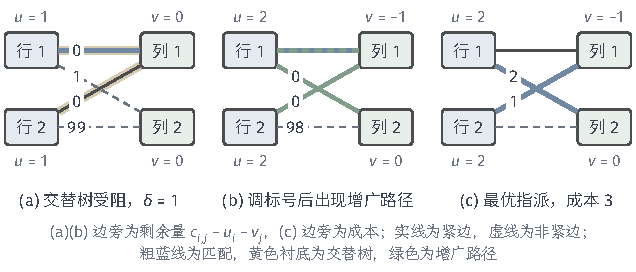
\includegraphics[width=107.714mm]{figures/01-basic-mathematics/04-graphs/tikz/c3-assign-hungarian/figure.pdf}
  \caption{匈牙利算法在成本矩阵$\left[\begin{smallmatrix}1&2\\1&100\end{smallmatrix}\right]$上的运行。行、列旁为当前标号。(a)匹配为行$1$配列$1$，从自由的行$2$出发的交替树（黄色衬底）只到达列$1$与行$1$，树外边的最小剩余量为$\delta=1$。(b)行标号加$1$、树中列标号减$1$后，行$1$到列$2$变紧，出现增广路径（绿色）。(c)翻转得到的指派成本为$3$，等于标号之和。}
  \label{fig:graph-opt-hungarian}
\end{figure}

\paragraph{停止与还原}
全部行都匹配后停止。若为矩形问题补过零成本虚拟行，删去它们的配对即得原问题的解；若按惩罚模型补过专属虚拟行列，配给专属虚拟对象的真实对象就是未配对的对象，总成本中相应的项就是它的惩罚。禁止的配对从未作为允许边出现，所以不会出现在结果中。

\subsection{算法分析与结果检验}
\label{sec:graph-opt-assign-analysis}

\paragraph{计算开销}
朴素地实现，每次调标号都要扫描$S$中全部行到树外全部列的剩余量。更好的做法是为每个未入树的列$j$维护最小剩余量$\min_{i\in S}(c_{i,j}-u_i-v_j)$及取到最小值的行，作为这一列的前驱。有一行加入$S$时，用它到各列的剩余量更新这些最小值，花$O(N)$；求$\delta$只需在这些最小值中再取最小，花$O(N)$；调标号后，未入树列的最小剩余量统一减去$\delta$，也是$O(N)$。为一个自由行建树直到增广，至多有$N$行加入$S$、至多调标号$N$次，所以一次增广为$O(N^2)$；至多增广$N$次，稠密$N$阶方阵上的总运算量为$O(N^3)$次实数运算。存储上，原始成本表占$N^2$个数，这是输入本身；算法额外的工作数组为$O(N)$。

\paragraph{结果检验}
先检查原始问题的可行性：每行恰配一个列，所用的列互不相同，全部配对都是允许边；再按原始成本重算总成本。然后检查证书：对全部允许边验证$u_i+v_j\leq c_{i,j}$，对所选的边验证取等号，并核对总成本等于$\sum_iu_i+\sum_jv_j$。原始可行解的成本等于标号下界，才构成最优性证书。浮点实现中，“紧”与“可行”都只能在容差内判断，应说明所用容差；近似相等不能无条件替代精确证书。

\paragraph{三种问题的比较}
最大匹配、指派与最小费用流可以互相转写，但目标与约束不同。最大匹配只求配对数量，边上没有成本；指派要求每个对象都完成配对，在这一条件下比较成本；最小费用流允许一般的容量、上下界与供需，指派只是全部容量为一、每行供给一、每列需求一的特例。图~\ref{fig:graph-opt-problem-relations}汇总了这些关系。专门算法保留了各自的结构：增广匹配只需记录配对伙伴，匈牙利算法的标号与交替树都利用了二部结构，网络单纯形法则适用于一般网络。算法名称不是不改模型就能互换的工具，换用另一种算法之前，须先把问题按它的输入要求重新写出。

\begin{figure}[!htb]
  \centering
  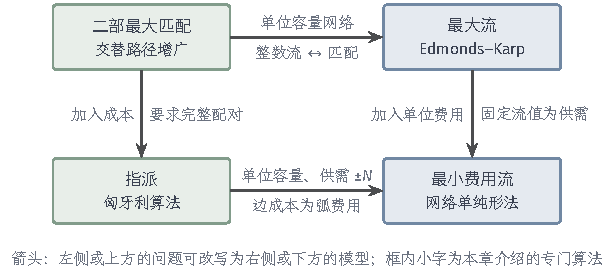
\includegraphics[width=103.914mm]{figures/01-basic-mathematics/04-graphs/tikz/c3-problem-relations/figure.pdf}
  \caption{本章四种流与配对问题之间的模型关系。箭头表示起点的问题可以写成终点的模型：二部最大匹配是单位容量的最大流，加入成本并要求完整配对就成为指派；最大流固定流值并加入单位费用就成为最小费用流，指派是单位容量的最小费用流。框内小字是本章为各问题介绍的专门算法。}
  \label{fig:graph-opt-problem-relations}
\end{figure}

% 第3章第7节：本章小结。

\section{本章小结}
\label{sec:graph-optimization-summary}

本章的六个问题都在有限图上从满足结构要求的候选中挑选数值最好者，但选择的对象和数值的含义各不相同。最短路选一条路径，比较弧长之和；最小生成树选一组连接全部顶点的边，比较建造成本之和；最大流给每条弧分配流量，在容量上界内最大化源汇之间的净输送量；最小费用流在供需固定时比较输送费用；匹配选互不共享端点的边，只数配对个数；指派要求每个对象都完成配对，再比较配对成本。同样写在边旁的一个数，可以是长度、成本、容量或单位费用，它们不能互换解释：例如最小生成树上两点间的路径未必是最短路，最大流也不关心沿哪条路线输送更便宜。

各算法依靠的论证与成立条件也不同。有向无环图上的递推依靠拓扑序，前驱的距离在使用前已经确定；Bellman--Ford算法允许负边长，靠“至多$k$条弧”的递推反复修正标签，并能识别负环的影响；Dijkstra算法只在边长非负时成立，每次永久确定一个顶点。Kruskal算法与Prim算法依靠割性质，用交换论证说明每次选的边可以留在某棵最优树中。最大流的Ford--Fulkerson方法与Edmonds--Karp算法沿残量网络中的增广路径增加流量，前者在整数容量下有限终止，后者按最少弧数选路，对实容量也给出增广次数的界。网络单纯形法沿树上的基本环调整流量，靠词典序规则排除零步长换基造成的循环。增广匹配沿交替路径翻转选边状态；匈牙利算法在紧边上增广，在受阻时调整标号。

许多算法停止时都留下一份可以独立核对的证书，表~\ref{tab:graph-opt-summary}把它们与输入条件、主要开销并列。最短路的证书是逐弧距离不等式；最大流的证书是同值的流与割；最小费用流的证书是流量与节点势满足的逐弧符号条件；最大匹配的证书是单位容量网络中与匹配边数同值的割；指派的证书是成本等于标号之和的紧边指派。最小生成树的最优性则回到割性质：每条非树边都不轻于它在树上所对应路径中的边。证书的价值在于检查者不必相信求解过程，只需核对可行性和若干不等式；浮点计算中这些核对都要带容差，近似满足不能直接当作精确证书。

\begin{table*}[!htb]
  \centering\small
  \caption{本章六个问题的对比（$n$为顶点数，$m$为无向边数，$a$为有向弧数，$\nu$为二部图较小一侧的顶点数，$N$为指派方阵的阶数）。开销均为本章所述实现的运算量。}
  \label{tab:graph-opt-summary}
  \begin{tabularx}{\linewidth}{@{}l>{\raggedright\arraybackslash}X>{\raggedright\arraybackslash}X>{\raggedright\arraybackslash}X>{\raggedright\arraybackslash}p{30mm}@{}}
    \toprule
    问题 & 选择对象与目标 & 方法与成立条件 & 结果证书 & 主要开销\\
    \midrule
    最短路 & 一条路径，弧长之和最小 & DAG递推（无有向环）；Bellman--Ford（允许负边，检测负环）；Dijkstra（边长非负） & 逐弧距离不等式与前驱路线 & $O(n+a)$；$O(na)$；$O((n+a)\log n)$\\
    最小生成树 & 连接全部顶点的边集，成本之和最小 & Kruskal、Prim，依靠割性质 & 无环、覆盖各分量；非树边不轻于树上对应路径的边 & $O(m\log m)$；$O(n^2+m)$或$O((n+m)\log n)$\\
    最大流 & 各弧流量，源汇净输送量最大 & 残量增广；整数容量下任意选路有限终止，按最少弧数选路对实容量成立 & 同值的流与割 & Edmonds--Karp为$O(na^2)$\\
    最小费用流 & 各弧流量，供需固定时费用最小 & 网络单纯形法：可行树基、基本环调整、两阶段初始化、词典序防循环 & 流量与节点势的逐弧符号条件 & 每轮$O(n+a)$，总轮数无统一多项式界\\
    二部最大匹配 & 互不共享端点的边，边数最多 & 交替路径增广，限于二部图 & 单位容量网络中同值的割 & $O(\nu(n+m))$\\
    指派 & 完美匹配，成本之和最小 & 匈牙利算法：可行标号与紧边匹配 & 成本等于标号之和 & $O(N^3)$\\
    \bottomrule
  \end{tabularx}
\end{table*}

本章的两种结构会在后面再次用到。把全部边权取负，或把选边次序改为从大到小，最小生成树的算法就求出最大权生成树；第~\ref{sec:graph-tree-decomposition-construction}节构造团树时，以极大团为顶点、团的交集大小为边权，调用的正是最大权生成树。最小割则在第~\ref{sec:graph-pairwise-binary-cut}节中用于最小化由一元项和成对项组成的二值函数：满足相应条件的目标可以写成割容量加常数，于是最大流算法给出精确的最小化配置。复用之前都要先说明问题怎样转成当前的网络与目标，不能只因为都用到图就共享最优性结论。

本章选择的始终是路径、树、流、匹配这类具有特定组合结构的对象，算法的正确性也来自这些结构本身的性质。下一章转而用集合函数评价一般的子集，候选对象可以是顶点、边、特征或传感器。那里将区分两种情形：一种是评价函数的一般性质（如收益递减）给出贪心选择的近似保证，另一种是特殊的表示（如可以写成图割）带来精确的求解。


\chapter{集合函数与子集选择}
\label{chap:graph-set-functions}

在一片区域里安装传感器时，每个候选位置都能覆盖一块范围，但相邻位置的覆盖范围往往重叠。选定一组位置后，真正有意义的是这组位置合起来覆盖了多少，而不是各自覆盖面积的简单相加。同样，从一批特征里挑出一组、从一张图里挑出一部分顶点，评价的对象都是整组选择。前一章选择的是路径、生成树、流和匹配这些具有特定结构的对象；本章把候选对象放进一个有限的底集，研究怎样评价它的子集、怎样从累计评价中恢复各部分的贡献，以及怎样在数量或预算限制下选出好的子集。底集可以是图的顶点，也可以是边、特征或传感器，所以本章是从图向一般离散选择的扩展。

第~\ref{sec:graph-set-function-basics}节把“给子集赋值”写成集合函数，用二值向量表示子集，并用新增一个元素前后的评价差定义边际增益。第~\ref{sec:graph-set-function-properties}节依次区分单调性、模性与次模性：它们分别回答新增元素会不会降低评价、各元素的贡献是否固定、以及收益是否随已选集合增大而递减。第~\ref{sec:comb-cumulative-inversion}节转向另一项任务：已知每个子集的累计评价，怎样恢复每个子集自身的贡献；这一节只用有限求和与包含关系，不依赖前一节的性质。

后半章讨论选择。第~\ref{sec:graph-cardinality-selection}节在“至多选$k$个”的限制下逐轮加入边际增益最大的元素，并证明目标单调且次模时，这样得到的值不低于最优值的$1-(1-1/k)^k$倍。第~\ref{sec:graph-budget-selection}节让不同元素占用不同的预算，说明按单位成本选择怎样改进、又会在什么例子中失效。第~\ref{sec:graph-pairwise-binary-cut}节换成最小化问题：当目标只由一元项和满足一定条件的成对项组成时，它可以表示为割的容量，并用第~\ref{sec:graph-max-flow}节的最小割精确求解。这三节按约束与目标结构分别组织，彼此不是一条必然的依赖链。

% 第4章第1节：集合函数（集合函数的定义；子集与二值向量；边际增益）。

\section{集合函数}
\label{sec:graph-set-function-basics}

给每个元素赋一个数，只需要一张长度为元素个数的表；给每个子集赋一个数，则要考虑元素之间怎样相互影响。本节先用传感器覆盖说明为什么需要以子集为自变量的函数，再把子集写成二值向量，最后定义新增一个元素带来的评价变化。这三样东西是后面判断函数性质、设计选择方法时共同使用的记号。

\subsection{集合函数的定义}
\label{sec:graph-setfn-definition}

\paragraph{传感器覆盖实例}
图~\ref{fig:graph-setfn-sensor-coverage}是一块由上下两行、左右八列组成的区域，共$16$个格子。有四个候选传感器：$a$覆盖第$2$至$6$列的$10$个格子，$b$覆盖第$1$至$4$列的$8$个格子，$c$覆盖第$5$至$8$列的$8$个格子，$d$只覆盖左上角的$1$个格子。选定一组传感器后，我们关心这组传感器合起来覆盖了多少个不同的格子。记传感器$v$覆盖的格子集合为$C_v$，选定的传感器集合为$S$，覆盖量就是
\[
  F(S)=\Bigl|\bigcup_{v\in S}C_v\Bigr|.
\]
单独看，$F(\{a\})=10$，$F(\{b\})=8$；两者一起时，第$2$至$4$列被重复覆盖，$F(\{a,b\})=12$，而不是$10+8=18$。整组的价值不能由各成员的价值相加得到，因此评价必须直接以“哪些传感器被选中”为输入。本章后面几节都用这个实例做算例。

\begin{figure}[!htb]
  \centering
  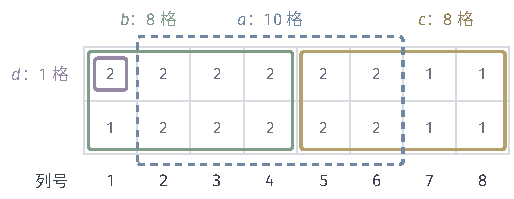
\includegraphics[width=87.027mm]{figures/01-basic-mathematics/04-graphs/tikz/c4-sensor-coverage/figure.pdf}
  \caption{贯穿本章的传感器覆盖实例。区域由$2\times 8$个格子组成；绿色框为$b$（第$1$至$4$列），黄色框为$c$（第$5$至$8$列），蓝色虚线框为$a$（第$2$至$6$列），紫色小框为$d$（左上角一格）。格内数字是覆盖该格的传感器个数，数字$2$所在的格子都被重复覆盖，因而各传感器覆盖格数之和大于它们合起来覆盖的格数。}
  \label{fig:graph-setfn-sensor-coverage}
\end{figure}

覆盖量的输入是一个子集，输出是一个实数。把这种对应一般化，就得到下面的定义。

\begin{definition}[集合函数]
\label{def:graph-setfn-set-function}
设$V$是有限集合，称为\term{底集}（ground set）。把$V$的每个子集对应到一个实数的映射
\[
  F:\mathcal P(V)\to\mathbb R
\]
称为$V$上的\term{集合函数}（set function），其中$\mathcal P(V)$是$V$的幂集。
\end{definition}

定义要求$F$在每个子集上都有值，包括空集。空集表示“什么都不选”，它的值是比较其他选择的起点：覆盖量取$F(\varnothing)=0$，一个带固定开销的评价则可能取非零值。底集中的元素可以是传感器、特征、顶点或边；集合函数本身并不要求底集带有图结构。

\paragraph{三个例子}
同一个子集可以按不同目的评价。以传感器实例为例，给四个传感器分别指定安装成本$4,3,4,1$（依次对应$a,b,c,d$），总成本
\[
  c(S)=\sum_{v\in S}c_v
\]
是一个集合函数，例如$c(\{a,b\})=7$；覆盖量$F$是另一个集合函数，$F(\{a,b\})=12$。第三个例子来自图。设$\mathcal G=(V,E)$是无向图，每条边$\{i,j\}$带非负权$w_{i,j}$。顶点子集$S$把顶点分成$S$与$V\setminus S$两侧，这正是第~\ref{sec:graph-minimum-spanning-tree}节所说的割；两端分居两侧的边的权之和
\[
  \operatorname{cut}(S)=\sum_{\{i,j\}\in E:\ |\{i,j\}\cap S|=1}w_{i,j}
\]
称为$S$的割权。这里的底集是顶点集，$\operatorname{cut}$以顶点子集为自变量。三个例子分别累计单项成本、合并覆盖范围和统计跨越两侧的边，元素之间的相互影响各不相同，下一节将据此区分它们的性质。

\paragraph{取值表与求值规则}
由式~\eqref{eq:comb-power-set-count}，$n$元底集有$2^n$个子集，所以一个集合函数的完整取值表有$2^n$项。传感器实例只有$16$项，可以全部写出；底集有$50$个元素时，取值表已超过$10^{15}$项，无法存储。实际问题中的集合函数通常由一条规则给出：给定$S$，按规则算出$F(S)$。覆盖量的规则是求并集再计数，割权的规则是扫描全部边。这样的一次计算称为一次\emph{求值}，它的代价取决于具体表示：覆盖量的一次求值要处理$S$中各传感器的覆盖范围，割权的一次求值要检查每条边。后面分析算法时，我们把求值次数和每次求值的代价分开计算，不把求值默认视为免费。

\subsection{子集与二值向量}
\label{sec:graph-setfn-binary-vectors}

给底集的元素固定编号$V=\{1,\ldots,n\}$。第~\ref{sec:comb-ordered-unordered}节已经说明，子集$S$与零一记录一一对应。把这条记录写成向量$\bm x=(x_1,\ldots,x_n)\in\{0,1\}^n$，其中
\[
  x_i=\mathbb I\{i\in S\},
\]
称$\bm x$为$S$的\term{指示向量}（indicator vector）。反过来，由$\bm x$恢复子集只需收集取值为$1$的坐标：$S=\{i:x_i=1\}$。

集合运算在指示向量上逐坐标进行。设$S,T$的指示向量为$\bm x,\bm y$，则元素个数是坐标之和，$|S|=\sum_ix_i$；并集的第$i$个坐标是$\max\{x_i,y_i\}$，交集的第$i$个坐标是$\min\{x_i,y_i\}=x_iy_i$，补集的第$i$个坐标是$1-x_i$。包含关系$S\subseteq T$对应逐坐标的$x_i\leq y_i$。

于是集合函数也可以写成二值向量的函数：令$f(\bm x)=F(\{i:x_i=1\})$，$f$与$F$只是同一组数值的两种索引方式。图~\ref{fig:graph-setfn-subset-binary-cube}以三元底集为例画出这一对应：八个子集恰好是立方体的八个顶点，立方体的每条边连接只差一个元素的两个子集，也就是只差一个坐标的两个向量。

\begin{figure}[!htb]
  \centering
  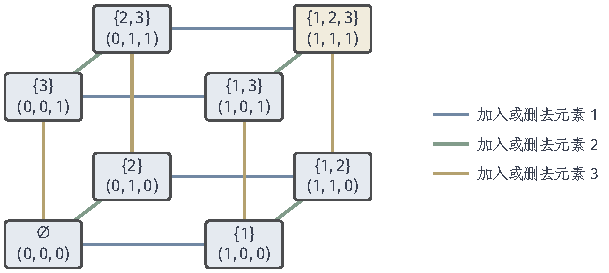
\includegraphics[width=103.209mm]{figures/01-basic-mathematics/04-graphs/tikz/c4-subset-binary-cube/figure.pdf}
  \caption{三元底集$V=\{1,2,3\}$的八个子集与指示向量$(x_1,x_2,x_3)$排成立方体的顶点。每个框上行是子集，下行是对应的向量；边的颜色表示沿这条边加入或删去哪个元素，也就是改变哪个坐标。沿任一条边向上走一步，就是在当前子集中加入一个元素。}
  \label{fig:graph-setfn-subset-binary-cube}
\end{figure}

这一改写只换了表示方式，并没有带来额外结构。写成$f(\bm x)$之后，$f$不一定是各坐标的函数之和，也不一定能分解成只读取少数坐标的局部项；在$\{0,1\}^n$上谈连续性或求导也没有意义。第~\ref{sec:graph-pairwise-binary-cut}节和第~\ref{chap:graph-dynamic-programming}章讨论的，正是函数确实具有某种局部分解时可以怎样利用它。

\subsection{边际增益}
\label{sec:graph-setfn-marginal-gain}

选择子集时，最直接的问题是：在已经选好的集合上再加一个元素，评价会改变多少。

\begin{definition}[边际增益]
\label{def:graph-setfn-marginal-gain}
设$F$是$V$上的集合函数，$S\subseteq V$，$v\in V\setminus S$。称
\[
  \Delta(v\mid S)=F(S\cup\{v\})-F(S)
\]
为元素$v$相对于集合$S$的\term{边际增益}（marginal gain）。
\end{definition}

边际增益同时依赖新元素和已选集合。图~\ref{fig:graph-setfn-marginal-gain-overlap}比较同一个传感器$c$在两种情况下的增益：从空集加入时，$c$的$8$个格子都是新覆盖的，$\Delta(c\mid\varnothing)=8$；已经选了$a$之后，$c$的第$5$、$6$列已被$a$覆盖，只有第$7$、$8$列的$4$个格子是新的，$\Delta(c\mid\{a\})=4$。所以谈论一个元素“值多少”时，必须说明是相对于哪个已选集合。

\begin{figure}[!htb]
  \centering
  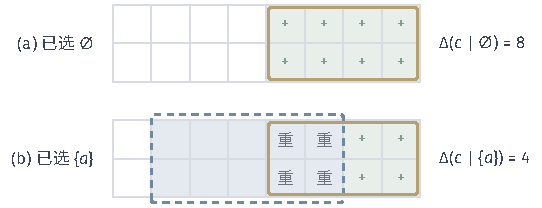
\includegraphics[width=91.74mm]{figures/01-basic-mathematics/04-graphs/tikz/c4-marginal-gain-overlap/figure.pdf}
  \caption{同一传感器$c$（黄色框）的边际增益随已选集合变化。(a) 已选集合为空，$c$覆盖的$8$个格子（绿色，标“$+$”）全部是新覆盖；(b) 已选$\{a\}$（蓝色底与蓝色虚线框），$c$与$a$重叠的第$5$、$6$列（标“重”）不再计数，只有第$7$、$8$列的$4$个格子是新覆盖。}
  \label{fig:graph-setfn-marginal-gain-overlap}
\end{figure}

\paragraph{逐个加入的累计}
把一个集合的元素逐个加入，函数的总变化就是一串边际增益之和。设$A\subseteq B\subseteq V$，把$B\setminus A$中的元素按任意次序排成$v_1,\ldots,v_r$，记$A_0=A$，$A_k=A\cup\{v_1,\ldots,v_k\}$。于是$A_r=B$，并且
\begin{equation}
  F(B)-F(A)=\sum_{k=1}^{r}\bigl(F(A_k)-F(A_{k-1})\bigr)=\sum_{k=1}^{r}\Delta(v_k\mid A_{k-1}).
  \label{eq:graph-setfn-telescoping}
\end{equation}
第一个等号是裂项求和（式~\eqref{eq:prelim-telescoping-sum}）：中间的$F(A_1),\ldots,F(A_{r-1})$各出现一次正号、一次负号而抵消。第二个等号是因为$A_k=A_{k-1}\cup\{v_k\}$且$v_k\notin A_{k-1}$。

在传感器实例中取$A=\varnothing$、$B=\{a,b,c\}$。按$a,c,b$的次序加入，三个增益依次是$10,4,2$；按$b,c,a$的次序加入，三个增益依次是$8,8,0$。两种次序的总和都是$F(\{a,b,c\})=16$，但每一步的增益随次序改变。式~\eqref{eq:graph-setfn-telescoping}是下一节判别性质和第~\ref{sec:graph-cardinality-selection}节分析贪心算法的共同工具。

边际增益只描述一步的变化。在空集上，$a$的增益$10$是四个传感器中最大的，但只能选两个传感器时，最好的组合是$\{b,c\}$，它覆盖全部$16$个格子，并不包含$a$。单步增益大，不保证这一步属于某个全局最优子集；这一点将在第~\ref{sec:graph-cardinality-selection}节具体比较。

% 第4章第2节：集合函数的性质（单调性；模性；次模性与超模性）。

\section{集合函数的性质}
\label{sec:graph-set-function-properties}

上一节的三个例子在“加入一个元素会怎样改变评价”这个问题上表现不同：加入传感器不会减少覆盖，但可能增加的覆盖越来越少；加入一项成本总是增加固定的数额；把一个顶点移到$S$一侧，割权可能增加也可能减少。本节把这些表现分别写成单调性、模性和次模性，并说明三者各有条件，不能互相推出。

\subsection{单调性}
\label{sec:graph-setfn-monotonicity}

多装一个传感器，覆盖的格子只会增加或保持不变。把这一性质写成子集之间的比较，就是下面的定义。

\begin{definition}[单调非减]
\label{def:graph-setfn-monotone}
若对任意$A\subseteq B\subseteq V$都有$F(A)\leq F(B)$，称集合函数$F$\term{单调非减}（monotone nondecreasing），简称单调。
\end{definition}

定义比较的是任意两个有包含关系的子集，检查起来要考虑很多对。借助式~\eqref{eq:graph-setfn-telescoping}，它可以化成只检查单个元素的条件：$F$单调，当且仅当对每个$S\subseteq V$和每个$v\notin S$都有$\Delta(v\mid S)\geq0$。必要性只需取$A=S$、$B=S\cup\{v\}$。充分性：对任意$A\subseteq B$，式~\eqref{eq:graph-setfn-telescoping}把$F(B)-F(A)$写成若干个边际增益之和，每一项都非负，所以$F(A)\leq F(B)$。

覆盖量是单调的：加入$v$后新增的格子数$\Delta(v\mid S)=|C_v\setminus\bigcup_{u\in S}C_u|$不会是负数。

\paragraph{单调性与非负性的区别}
覆盖量含在一个目标里，并不保证整个目标单调。把覆盖量减去安装成本，得到净收益$G(S)=F(S)-c(S)$。$G(\{b\})=8-3=5$，而$G(\{b,d\})=8-4=4$：$d$覆盖的那一格已被$b$覆盖，加入$d$不增加覆盖，却多花$1$个单位成本，所以净收益下降。

函数值全为非负，也不能推出单调。在二元底集$\{1,2\}$上取
\[
  F(\varnothing)=1,\quad F(\{1\})=3,\quad F(\{2\})=2,\quad F(\{1,2\})=2,
\]
四个值都是正数，但$\Delta(2\mid\{1\})=2-3=-1<0$。反过来，单调也不能推出$F(\varnothing)=0$：常数函数$F\equiv5$是单调的。$F(\varnothing)=0$称为\emph{归一化}，它是一项约定；对任意集合函数，减去常数$F(\varnothing)$就得到归一化的函数，而所有边际增益保持不变。归一化且单调的函数必然处处非负，因为$F(S)\geq F(\varnothing)=0$。

\subsection{模性}
\label{sec:graph-setfn-modularity}

总成本$c(S)$具有最简单的结构：每个元素贡献一个固定的数，彼此互不影响。一般地，取常数$c_0$和每个元素的权$w_v$，令
\begin{equation}
  F(S)=c_0+\sum_{v\in S}w_v .
  \label{eq:graph-setfn-modular-form}
\end{equation}
这时对任意$S$和$v\notin S$，$\Delta(v\mid S)=w_v$，增益与已选集合无关。由上一小节的判别条件，这样的$F$单调当且仅当每个$w_v\geq0$；常数$c_0$不影响任何边际增益。

\paragraph{模等式}
对形如式~\eqref{eq:graph-setfn-modular-form}的函数和任意两个子集$A,B$，比较$F(A)+F(B)$与$F(A\cup B)+F(A\cap B)$。两边都含两个常数$c_0$。对一个元素$v$：若$v$同时属于$A$和$B$，则$w_v$在左边计两次，在右边的并集与交集中也各计一次；若$v$只属于其中一个，则$w_v$在两边都只计一次；若$v$都不属于，则两边都不计。所以
\begin{equation}
  F(A)+F(B)=F(A\cup B)+F(A\cap B).
  \label{eq:graph-setfn-modular-equality}
\end{equation}
对所有$A,B\subseteq V$满足式~\eqref{eq:graph-setfn-modular-equality}的集合函数称为\term{模函数}（modular function）。

反过来，模等式也足以恢复固定权重的表示，因此它可以用来判断元素之间有没有交互。设$F$是模函数，取$S\neq\varnothing$与$v\in S$，在式~\eqref{eq:graph-setfn-modular-equality}中令$A=S\setminus\{v\}$、$B=\{v\}$，这时$A\cup B=S$，$A\cap B=\varnothing$，得到
\[
  F(S)=F(S\setminus\{v\})+\bigl(F(\{v\})-F(\varnothing)\bigr).
\]
对$|S|$归纳，就得到$F(S)=F(\varnothing)+\sum_{v\in S}\bigl(F(\{v\})-F(\varnothing)\bigr)$，即式~\eqref{eq:graph-setfn-modular-form}取$c_0=F(\varnothing)$、$w_v=F(\{v\})-F(\varnothing)$。覆盖量不是模函数：$F(\{a\})+F(\{b\})=18$，而$F(\{a,b\})+F(\varnothing)=12$，差值$6$正是两者重叠的格子数。

\subsection{次模性}
\label{sec:graph-setfn-submodularity}

覆盖量的增益随已选集合增大而变小：已覆盖的格子越多，新传感器能补上的格子越少。图~\ref{fig:graph-setfn-marginal-gain-overlap}中，$\Delta(c\mid\varnothing)=8$，$\Delta(c\mid\{a\})=4$；再加入$b$之后，$\Delta(c\mid\{a,b\})=4$，没有继续变小，但也没有变大。把“不会变大”作为要求，就得到边际收益递减的条件。

\begin{definition}[次模函数]
\label{def:graph-setfn-submodular}
若对任意$A\subseteq B\subseteq V$和任意$v\in V\setminus B$都有
\begin{equation}
  \Delta(v\mid A)\geq\Delta(v\mid B),
  \label{eq:graph-setfn-diminishing-returns}
\end{equation}
称集合函数$F$是\term{次模}函数（submodular function）。
\end{definition}

条件中的$v$不属于$B$，从而也不属于$A$，两个增益都有定义。次模性还有一种不出现边际增益的写法，它和模等式形式相同，只是把等号换成不等号。

\begin{theorem}[次模性的两种刻画]
\label{thm:graph-setfn-submodular-equivalence}
设$V$是有限集合，$F$是$V$上的集合函数。$F$满足式~\eqref{eq:graph-setfn-diminishing-returns}，当且仅当对任意$X,Y\subseteq V$都有
\begin{equation}
  F(X)+F(Y)\geq F(X\cup Y)+F(X\cap Y).
  \label{eq:graph-setfn-submodular-inequality}
\end{equation}
\end{theorem}

\begin{proof}
先设式~\eqref{eq:graph-setfn-submodular-inequality}成立。给定$A\subseteq B$和$v\notin B$，取$X=A\cup\{v\}$、$Y=B$。由$A\subseteq B$得$X\cup Y=B\cup\{v\}$；由$v\notin B$得$X\cap Y=A$。代入式~\eqref{eq:graph-setfn-submodular-inequality}，
\[
  F(A\cup\{v\})+F(B)\geq F(B\cup\{v\})+F(A),
\]
移项即$\Delta(v\mid A)\geq\Delta(v\mid B)$。

再设式~\eqref{eq:graph-setfn-diminishing-returns}成立。给定$X,Y$，记$C=X\cap Y$，把$Y\setminus X$中的元素按任意次序排成$y_1,\ldots,y_r$。分别从$X$和从$C$出发逐个加入这些元素，由式~\eqref{eq:graph-setfn-telescoping}，
\[
  \begin{gathered}
  F(X\cup Y)-F(X)=\sum_{k=1}^{r}\Delta\bigl(y_k\mid X\cup\{y_1,\ldots,y_{k-1}\}\bigr),\\
  F(Y)-F(C)=\sum_{k=1}^{r}\Delta\bigl(y_k\mid C\cup\{y_1,\ldots,y_{k-1}\}\bigr).
  \end{gathered}
\]
这里用到$X\cup(Y\setminus X)=X\cup Y$与$C\cup(Y\setminus X)=Y$。对每个$k$，$C\cup\{y_1,\ldots,y_{k-1}\}\subseteq X\cup\{y_1,\ldots,y_{k-1}\}$，且$y_k$不属于后者（$y_k\notin X$，并且与前面的$y_j$不同）。由式~\eqref{eq:graph-setfn-diminishing-returns}，第二个和的每一项不小于第一个和的对应项，所以$F(X\cup Y)-F(X)\leq F(Y)-F(C)$，移项即得式~\eqref{eq:graph-setfn-submodular-inequality}。
\end{proof}

两种刻画各有用处：式~\eqref{eq:graph-setfn-diminishing-returns}直接对应“收益递减”的直观，适合分析逐个加入元素的算法；式~\eqref{eq:graph-setfn-submodular-inequality}只涉及四个函数值，适合验证具体函数。模函数在式~\eqref{eq:graph-setfn-submodular-inequality}中处处取等号，所以模函数是次模的。

\paragraph{覆盖量是次模的}
设$A\subseteq B$，$v\notin B$。$v$相对于$S$的增益是$C_v$中尚未被$S$覆盖的格子数，即$\Delta(v\mid S)=|C_v\setminus U(S)|$，其中$U(S)=\bigcup_{u\in S}C_u$。由$A\subseteq B$得$U(A)\subseteq U(B)$，于是$C_v\setminus U(B)\subseteq C_v\setminus U(A)$，取元素个数就得到式~\eqref{eq:graph-setfn-diminishing-returns}。这个论证不依赖格子的具体排列，所以任何“覆盖了多少个不同对象”的函数都是次模的，称为\term{覆盖函数}（coverage function）。

\paragraph{割权是次模的}
割权按边累加，所以先看一条权为$w$的边$\{i,j\}$单独贡献的函数：它在$S$恰含$i,j$之一时取$w$，否则取$0$。对不是端点的元素，这条边的贡献不随它的加入而改变，增益为$0$。加入端点$i$时，若$j$已在集合中，这条边从跨越两侧变为两端同侧，增益为$-w$；若$j$不在集合中，这条边从两端同侧变为跨越两侧，增益为$+w$。

现在取$A\subseteq B$、$i\notin B$，按$j$的归属分三种情形比较两个增益，见图~\ref{fig:graph-setfn-cut-submodular-cases}。若$j\in A$，则$j$也在$B$中，两个增益都是$-w$；若$j\in B\setminus A$，则$\Delta(i\mid A)=+w$而$\Delta(i\mid B)=-w$；若$j\notin B$，两个增益都是$+w$。三种情形都满足$\Delta(i\mid A)\geq\Delta(i\mid B)$，所以单条边的贡献是次模的。若干个函数各自满足式~\eqref{eq:graph-setfn-diminishing-returns}时，把这些不等式逐项相加，可知它们的和也满足，于是$\operatorname{cut}$作为各边贡献之和也是次模的。边权非负在这里是必要的：若某条边的权为负，第二种情形的不等号就反向了。

\begin{figure}[!htb]
  \centering
  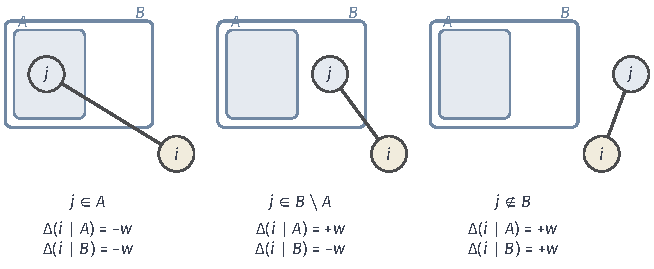
\includegraphics[width=110.723mm]{figures/01-basic-mathematics/04-graphs/tikz/c4-cut-submodular-cases/figure.pdf}
  \caption{割权函数次模性的逐边验证。固定一条权为$w\geq0$的边$\{i,j\}$，已选集合$A\subseteq B$（内框为$A$，外框为$B$），待加入的端点$i$（黄色）不在$B$中。按另一端点$j$的位置分三种情形：$j\in A$时两个增益都是$-w$；$j\in B\setminus A$时$A$上增益为$+w$、$B$上增益为$-w$；$j\notin B$时两个增益都是$+w$。每种情形都有$\Delta(i\mid A)\geq\Delta(i\mid B)$。}
  \label{fig:graph-setfn-cut-submodular-cases}
\end{figure}

\paragraph{次模与单调互不蕴含}
割权常常随集合增大而下降：$\operatorname{cut}(\varnothing)=\operatorname{cut}(V)=0$，而中间的子集可以有正的割权。图~\ref{fig:graph-setfn-property-counterexamples}(b)是只有一条权$1$的边的情形，割权依次为$0,1,1,0$，从单元素集到$\{1,2\}$时下降，所以次模函数不必单调。反方向，图~\ref{fig:graph-setfn-property-counterexamples}(a)的函数
\[
  F(S)=\max\bigl\{3\,\mathbb I\{\{1,2\}\subseteq S\},\ \mathbb I\{3\in S\}\bigr\}
\]
是单调的，但$\Delta(2\mid\varnothing)=0<3=\Delta(2\mid\{1\})$，违反式~\eqref{eq:graph-setfn-diminishing-returns}，所以单调函数也不必次模。

\begin{figure}[!htb]
  \centering
  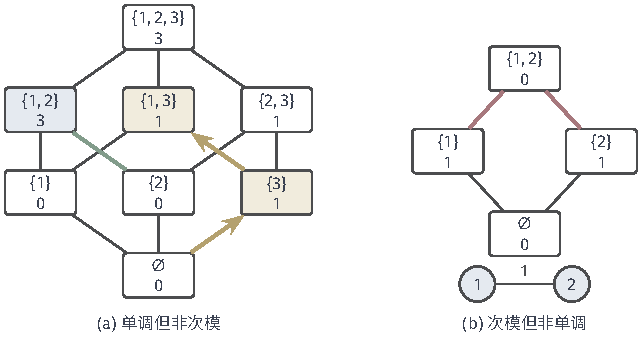
\includegraphics[width=108.687mm]{figures/01-basic-mathematics/04-graphs/tikz/c4-property-counterexamples/figure.pdf}
  \caption{单调性与次模性互不蕴含。每个框上行是子集，下行是函数值，连线连接只差一个元素的子集。(a) $F(S)=\max\{3\,\mathbb I\{\{1,2\}\subseteq S\},\mathbb I\{3\in S\}\}$：沿任一连线向上函数值不减，但绿色连线$\{2\}\to\{1,2\}$的增益$3$大于从空集加入$2$的增益$0$；黄色箭头是第~\ref{sec:graph-cardinality-selection}节贪心选择的路径，蓝色框是两元素时的最优集合。(b) 单条权$1$的边上的割权：次模，但红色连线上函数值从$1$降到$0$。}
  \label{fig:graph-setfn-property-counterexamples}
\end{figure}

\paragraph{超模性与协同}
把式~\eqref{eq:graph-setfn-diminishing-returns}的不等号反过来，即要求$\Delta(v\mid A)\leq\Delta(v\mid B)$，得到的函数称为\term{超模}函数（supermodular function）；等价地，$F$超模当且仅当$-F$次模。超模描述的是协同：两个部件只有同时具备才能工作时，单独加入任何一个的增益都是$0$，在另一个已经存在时加入，增益才是正的。例如$F(S)=\mathbb I\{\{1,2\}\subseteq S\}$是超模的。图~\ref{fig:graph-setfn-property-counterexamples}(a)的函数既不是次模也不是超模：元素$1,2$之间是协同的，而元素$3$与$\{1,2\}$之间是替代的，$\Delta(3\mid\varnothing)=1>0=\Delta(3\mid\{1,2\})$。

单调、模、次模、超模分别约束不同的东西，覆盖量、割权、净收益和上面的反例说明它们可以以各种方式组合出现。后面各节的算法保证都会同时写明目标是最大化还是最小化、函数是否单调、是否次模，以及约束是什么；只凭“次模”二字，并不能决定应当采用哪种方法。

% 第4章第3节：子集累计与 Möbius 反演（子集格与累计；Möbius 反演；反演的计算与算例；有限偏序集上的推广）。

\section{子集累计与 Möbius 反演}
\label{sec:comb-cumulative-inversion}

本节转向另一类问题。设想每个课程组合有一个总得分：单门课各有自己的贡献，某两门课同时选又会产生额外的配合效果，配合也可能是负的。我们能观察到的是每个组合的总得分，想知道的却是每个组合\emph{自身}贡献了多少。第~\ref{sec:comb-overlap-counting}节的容斥原理由各交集的大小恢复并集的大小，这里要做的是同一类“由累计量恢复局部量”的事，只是对象换成了一般的数值。本节只用有限求和与包含关系，不依赖上一节的单调或次模假设，也不是后面选择算法的前提。

\subsection{子集格与累计}
\label{sec:graph-setfn-subset-lattice}

累计沿包含关系进行，所以先把包含关系画出来。第~\ref{sec:prelim-order-relations}节已经说明，包含关系是幂集上的偏序。有限集合$V$的全部子集连同包含关系称为$V$的\term{子集格}（subset lattice）：两个子集的交是它们最大的公共子集，并是包含两者的最小集合。图~\ref{fig:comb-mobius-cumulative-local}按元素个数自下而上分层画出$V_0=\{1,2,3,4\}$的子集格，每条连线连接只差一个元素的两个子集，沿连线向上一步就是加入一个元素。图~\ref{fig:graph-setfn-subset-binary-cube}中的立方体正是三元底集的子集格。

从$S$出发沿连线一路向下能到达的子集，恰好是$S$的全部子集。例如从$\{1,3\}$向下只能到达$\{1\}$、$\{3\}$和空集。下面定义的累计值，正是沿这些向下的路径收集贡献。

\begin{figure}[!htb]
  \centering
  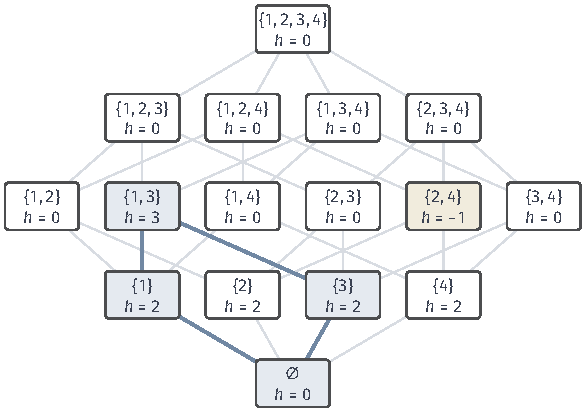
\includegraphics[width=99.187mm]{figures/01-basic-mathematics/04-graphs/tikz/c4-subset-lattice-cumulative/figure.pdf}
  \caption{四元素集合$V_0=\{1,2,3,4\}$的子集格与各子集自身的贡献$h$。子集按元素个数自下而上分层，连线连接只差一个元素的两个子集；框内上行为子集，下行为教学设定的贡献。蓝色标出$\{1,3\}$及其全部子集，它们的贡献相加得到累计值$g(\{1,3\})=0+2+2+3=7$；黄色框$\{2,4\}$的自身贡献为负。}
  \label{fig:comb-mobius-cumulative-local}
\end{figure}

\paragraph{自身贡献与累计值}
给每个子集$T$指定一个实数$h(T)$，表示$T$作为整体\emph{自身}带来的贡献：单元素集的贡献是单门课的得分，二元集的贡献是两门课的配合效果，依此类推。$S$的累计值收集它的全部子集的贡献：
\begin{equation}
  g(S)=\sum_{T\subseteq S}h(T).
  \label{eq:comb-zeta-transform}
\end{equation}
$g$与$h$都是$V$上的集合函数。注意累计不只相加单元素的贡献，$S$内部更大子集的配合贡献也计入其中。

图~\ref{fig:comb-mobius-cumulative-local}的教学设定让四个单项各贡献$2$，$\{1,3\}$另有配合贡献$3$，$\{2,4\}$另有配合贡献$-1$，其余子集（包括空集和全部三元、四元子集）的贡献为$0$。于是
\[
  g(\{1,3\})=h(\varnothing)+h(\{1\})+h(\{3\})+h(\{1,3\})=0+2+2+3=7,
\]
而两个单项的累计值之和只有$g(\{1\})+g(\{3\})=4$，多出的$3$正是$\{1,3\}$自身的贡献。反演要回答相反方向的问题：只知道每个子集的累计值$g$，怎样读出每个子集自身的贡献$h$。

\subsection{Möbius 反演}
\label{sec:graph-setfn-mobius-inversion}

先看两元素的情形。$g(\{1,3\})$包含$h(\varnothing)$、$h(\{1\})$、$h(\{3\})$和$h(\{1,3\})$四项。减去$g(\{1\})=h(\varnothing)+h(\{1\})$和$g(\{3\})=h(\varnothing)+h(\{3\})$，两个单项贡献被去掉，但$h(\varnothing)$被多减了一次，再加回$g(\varnothing)=h(\varnothing)$，剩下的恰是
\[
  h(\{1,3\})=g(\{1,3\})-g(\{1\})-g(\{3\})+g(\varnothing).
\]
符号按子集比$S$少几个元素交替变化。一般情形的公式正是这样，称为\term{Möbius反演}（Möbius inversion）。

\begin{theorem}[子集格上的 Möbius 反演]
\label{thm:comb-mobius-inversion}
设$V$为有限集合，$g,h:\mathcal P(V)\to\mathbb R$。若对每个$S\subseteq V$式~\eqref{eq:comb-zeta-transform}成立，则对每个$S\subseteq V$有
\begin{equation}
  h(S)=\sum_{T\subseteq S}(-1)^{|S|-|T|}g(T).
  \label{eq:comb-mobius-inversion}
\end{equation}
反过来，若对每个$S$式~\eqref{eq:comb-mobius-inversion}成立，则式~\eqref{eq:comb-zeta-transform}也对每个$S$成立。
\end{theorem}

\begin{proof}
把式~\eqref{eq:comb-zeta-transform}代入式~\eqref{eq:comb-mobius-inversion}右侧，得到对全部满足$R\subseteq T\subseteq S$的集合对$(R,T)$的双重和。先固定$T$再取$R$，与先固定$R$再取$T$，遍历的是同一批集合对，所以可以像第~\ref{sec:prelim-finite-sums-products}节的三角形求和那样交换有限求和的次序：
\[
  \sum_{T\subseteq S}(-1)^{|S|-|T|}\sum_{R\subseteq T}h(R)
  =\sum_{R\subseteq S}h(R)\sum_{T:\,R\subseteq T\subseteq S}(-1)^{|S|-|T|}.
\]
固定$R$后，满足$R\subseteq T\subseteq S$的$T$由$S\setminus R$中哪些元素被加入决定，即$T=R\cup D$，$D\subseteq S\setminus R$任意，且$|S|-|T|=|S\setminus R|-|D|$。记$q=|S\setminus R|$，按$|D|=j$分组，大小为$j$的$D$有$\binom qj$个，所以内层和等于
\[
  \sum_{j=0}^{q}\binom qj(-1)^{q-j}=(-1)^q\sum_{j=0}^{q}(-1)^j\binom qj
  =\begin{cases}1,&q=0,\\0,&q\geq1,\end{cases}
\]
最后一步用式~\eqref{eq:comb-alternating-subset-count}。内层和只在$R=S$时为$1$，在$R$是$S$的真子集时为$0$，所以真子集上的贡献全部抵消，右侧只剩$h(S)$。

反方向同样直接核对。由式~\eqref{eq:comb-mobius-inversion}给出$h$，代入$\sum_{T\subseteq S}h(T)$并交换求和次序，
\[
  \sum_{T\subseteq S}h(T)=\sum_{R\subseteq S}g(R)\sum_{T:\,R\subseteq T\subseteq S}(-1)^{|T|-|R|}.
\]
仍写$T=R\cup D$，内层和等于$\sum_{j=0}^{q}(-1)^j\binom qj$，它在$R=S$时只有$D=\varnothing$一项而等于$1$，在$R\neq S$时为$0$。所以右侧等于$g(S)$。
\end{proof}

定理说明式~\eqref{eq:comb-zeta-transform}与式~\eqref{eq:comb-mobius-inversion}是一对互逆的变换：从贡献到累计，再从累计回到贡献，不丢失任何信息。证明中起作用的是组合数的交错和为零，这与容斥原理的证明相同。区别在于，容斥最终使并集中的每个元素恰计一次，反演最终只保留指定子集自身的贡献。

\subsection{反演的计算与算例}
\label{sec:graph-setfn-mobius-computation}

\paragraph{四元素算例}
记$\mathbb I\{\cdot\}$为条件成立时取$1$、否则取$0$的指示函数。沿用图~\ref{fig:comb-mobius-cumulative-local}的设定，累计值可以写成
\[
  g(S)=2|S|+3\,\mathbb I\{\{1,3\}\subseteq S\}-\mathbb I\{\{2,4\}\subseteq S\}.
\]
其中$2|S|$收集$S$中各单项的贡献，后两项在$S$包含$\{1,3\}$或$\{2,4\}$时计入相应的配合贡献。表~\ref{tab:comb-four-element-mobius}列出全部$16$个累计值，以及只用这些累计值按式~\eqref{eq:comb-mobius-inversion}恢复的贡献。

\begin{table}[!htb]
  \centering
  \begin{tabular}{ccc@{\qquad}ccc}
    \toprule
    $S$ & $g(S)$ & $h(S)$ & $S$ & $g(S)$ & $h(S)$ \\
    \midrule
    $\varnothing$ & $0$ & $0$ & $\{2,3\}$ & $4$ & $0$ \\
    $\{1\}$ & $2$ & $2$ & $\{2,4\}$ & $3$ & $-1$ \\
    $\{2\}$ & $2$ & $2$ & $\{3,4\}$ & $4$ & $0$ \\
    $\{3\}$ & $2$ & $2$ & $\{1,2,3\}$ & $9$ & $0$ \\
    $\{4\}$ & $2$ & $2$ & $\{1,2,4\}$ & $5$ & $0$ \\
    $\{1,2\}$ & $4$ & $0$ & $\{1,3,4\}$ & $9$ & $0$ \\
    $\{1,3\}$ & $7$ & $3$ & $\{2,3,4\}$ & $5$ & $0$ \\
    $\{1,4\}$ & $4$ & $0$ & $V_0$ & $10$ & $0$ \\
    \bottomrule
  \end{tabular}
  \caption{四元素子集格上的累计值$g$与由式~\eqref{eq:comb-mobius-inversion}恢复的自身贡献$h$。恢复结果与教学设定一致：四个单项各为$2$，$\{1,3\}$为$3$，$\{2,4\}$为$-1$，其余子集（包括全部三元子集和$V_0$）均为$0$。}
  \label{tab:comb-four-element-mobius}
\end{table}

两个二元子集的贡献按上一小节的四项公式恢复：
\[
  h(\{1,3\})=7-2-2+0=3,\qquad h(\{2,4\})=3-2-2+0=-1.
\]
三元子集要用到八个累计值。对$S=\{1,2,3\}$，按子集大小依次取三元、二元、一元和空集项，
\[
  h(\{1,2,3\})=9-(4+7+4)+(2+2+2)-0=0.
\]
虽然$\{1,2,3\}$包含有配合效果的$\{1,3\}$，它的累计值$9$也大于三个单项之和$6$，但多出的$3$已经由$h(\{1,3\})$解释，三门课之间没有新的整体效果，所以三元贡献为$0$。$\{1,3,4\}$也是如此：$g=9$，恢复出$h=0$。反演还允许贡献为负，$h(\{2,4\})=-1$就是一例。

\paragraph{按子集大小递推}
式~\eqref{eq:comb-mobius-inversion}给出每个$h(S)$的显式公式。另一种做法直接由式~\eqref{eq:comb-zeta-transform}移项：
\[
  h(S)=g(S)-\sum_{T\subsetneq S}h(T).
\]
输入是全部$2^n$个累计值；从$h(\varnothing)=g(\varnothing)$出发，按元素个数从小到大计算，算到$S$时它的全部真子集的$h$都已求出；输出是全部$2^n$个贡献。在上面的算例中，先得到空集和四个单项，再由$h(\{1,3\})=7-(0+2+2)=3$等算出二元贡献，最后算三元与四元贡献。

两种做法的开销相同。处理$S$时都要遍历它的$2^{|S|}$个子集，按大小分组求和，总次数为
\[
  \sum_{k=0}^{n}\binom nk2^k=3^n,
\]
最后一步是二项式定理。输入本身已有$2^n$个数，所以这里没有多项式规模的算法：单个递推式写起来简短，并不意味着整个问题便宜。

若要进一步减少运算，可以逐个元素做差分：对$i=1,\ldots,n$依次执行“对每个含$i$的$S$，把当前存储的值$g(S)$替换为$g(S)-g(S\setminus\{i\})$”（同一轮中用的都是上一轮的值）。对$i$归纳可以核对，处理完元素$1,\ldots,i$后，$S$处存储的值等于$\sum(-1)^{|S|-|T|}g(T)$，其中$T$取遍满足$T\subseteq S$且与$S$在元素$i+1,\ldots,n$上一致的子集；$i=n$时这正是式~\eqref{eq:comb-mobius-inversion}。每轮做$2^{n-1}$次减法，总共$n2^{n-1}$次，仍随$n$指数增长，只是比$3^n$小。

\subsection{有限偏序集上的推广}
\label{sec:graph-setfn-poset-mobius}

反演公式中的系数$(-1)^{|S|-|T|}$只依赖两个子集的相对位置。同样的问题可以在任意有限偏序集$(X,\preceq)$上提出：给每个元素$y$一个数$h(y)$，沿下方累计得$g(x)=\sum_{y\preceq x}h(y)$，再问怎样由$g$恢复$h$。这时系数不再一律是$\pm1$，而由下面的函数确定。

\begin{definition}[Möbius 函数]
\label{def:graph-setfn-mobius-function}
设$(X,\preceq)$是有限偏序集，记$y\prec x$表示$y\preceq x$且$y\neq x$。偏序集的\term{Möbius函数}（Möbius function）$\mu$对满足$y\preceq x$的元素对定义为
\[
  \mu(y,y)=1,\qquad \mu(y,x)=-\sum_{z:\,y\preceq z\prec x}\mu(y,z)\quad(y\prec x),
\]
对不满足$y\preceq x$的元素对取$\mu(y,x)=0$。
\end{definition}

定义固定区间的下端$y$，从对角值$\mu(y,y)=1$出发向上递推：区间$\{z:y\preceq z\preceq x\}$越长，需要的已知值越多，而有限偏序集保证递推在有限步内完成。递推式移项后写成
\[
  \sum_{z:\,y\preceq z\preceq x}\mu(y,z)=0\qquad(y\prec x),
\]
即每个非平凡区间上的系数之和为零。这正是反演证明中内层和所需的抵消，所以按与定理~\ref{thm:comb-mobius-inversion}相同的交换求和论证，可以得到$h(x)=\sum_{y\preceq x}\mu(y,x)g(y)$。

\paragraph{子集格的系数}
在子集格上取$\mu(T,S)=(-1)^{|S|-|T|}$。对$T\subsetneq S$，记$q=|S\setminus T|\geq1$，
\[
  \sum_{R:\,T\subseteq R\subseteq S}(-1)^{|R|-|T|}=\sum_{j=0}^{q}(-1)^j\binom qj=0,
\]
这正是上面的递推式。所以子集格上的反演系数只取$\pm1$，式~\eqref{eq:comb-mobius-inversion}是一般结构的特例。

\paragraph{整除偏序的例子}
图~\ref{fig:graph-setfn-mobius-divisors}是$12$的六个正因数在整除关系下的偏序。从$\mu(1,1)=1$出发，$\mu(1,2)=\mu(1,3)=-1$；区间$\{1,2,4\}$是一条链，$\mu(1,4)=-(1-1)=0$；区间$\{1,2,3,6\}$与两元素的子集格形状相同，$\mu(1,6)=-(1-1-1)=1$；最后$\mu(1,12)=-(1-1-1+0+1)=0$。系数出现了$0$，说明一般偏序上的反演确实不同于子集格上的交错加减。本小节只作为有限组合结构的补充，不涉及无限偏序和收敛问题，后面的选择算法也不以它为前提。

\begin{figure}[!htb]
  \centering
  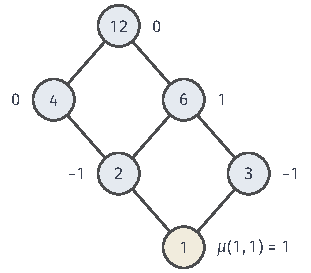
\includegraphics[width=52.613mm]{figures/01-basic-mathematics/04-graphs/tikz/c4-mobius-divisor-poset/figure.pdf}
  \caption{$12$的正因数在整除关系下的偏序，连线连接直接相邻的两个因数，下方整除上方。节点旁的数是$\mu(1,x)$，由$\mu(1,1)=1$（黄色节点）自下而上递推得到。链$1\mid2\mid4$上$\mu(1,4)=0$，与子集格同形的区间$\{1,2,3,6\}$上$\mu(1,6)=1$。}
  \label{fig:graph-setfn-mobius-divisors}
\end{figure}

% 第4章第4节：基数约束下的子集选择（基数约束与选择目标；边际增益贪心算法；贪心保证与适用范围）。

\section{基数约束下的子集选择}
\label{sec:graph-cardinality-selection}

回到传感器。预算只允许安装$k$个传感器时，应当选哪几个？本节先把目标、可行集合和函数的给定方式写清楚，再介绍逐轮加入边际增益最大元素的贪心算法，最后证明目标单调且次模时这种算法的近似保证，并用反例说明撤去条件后保证怎样失效。

\subsection{基数约束与选择目标}
\label{sec:graph-setfn-cardinality-problem}

设$V$是$n$元底集，$F$是$V$上的集合函数，整数$k$满足$0\leq k\leq n$。要求的是
\begin{equation}
  \max_{S\subseteq V,\ |S|\leq k}F(S).
  \label{eq:graph-setfn-cardinality-problem}
\end{equation}
“至多选$k$个”称为\term{基数约束}（cardinality constraint）。函数$F$通过求值规则给出：算法可以对任意子集询问$F$的值，每次询问计一次求值。

对单调函数，“至多$k$个”与“恰好$k$个”给出同样的最优值。若某个最优集合不足$k$个元素，任意补入元素使它恰有$k$个，由单调性函数值不会下降，补足后的集合仍是最优的。非单调函数不能这样处理：补入的元素可能降低目标值，所以“至多”与“恰好”是两个不同的问题。

\paragraph{枚举作为基准}
小底集可以枚举全部可行子集。在传感器实例中取$k=2$，可行子集有$\binom40+\binom41+\binom42=11$个。逐个计算覆盖量，最优值是$16$，最优集合唯一，为$\{b,c\}$；单元素中最好的是$\{a\}$，覆盖$10$格。一般地，最优值是唯一的，最优集合却可能有多个并列；$k=3$时，$\{b,c\}$、$\{a,b,c\}$、$\{b,c,d\}$都覆盖全部$16$个格子，按“至多$3$个”的约束三者都是最优集合。

枚举在规模稍大时就不可行。即使一次求值很便宜，$n=100$、$k=10$时，仅恰有$10$个元素的子集就有$\binom{100}{10}\approx1.7\times10^{13}$个。我们需要一种只看少量子集、利用边际增益结构逐步构造解的方法。

\subsection{边际增益贪心算法}
\label{sec:graph-setfn-greedy}

最自然的逐步构造是：每一轮在尚未选中的元素里，挑当前增益最大的那个加入。这里的“当前”很关键，增益要相对于已经选好的集合重新计算。

\begin{algorithm}[基数约束下的边际增益贪心]
\label{alg:graph-setfn-greedy}
输入：有限底集$V$（元素已编号），整数$0\leq k\leq|V|$，单调非减集合函数$F$的求值规则。输出：至多含$k$个元素的集合。状态：当前已选集合$S_{t-1}$及其函数值，本轮各候选元素的增益。
\begin{enumerate}
  \item 令$S_0=\varnothing$，记录$F(S_0)$。
  \item 对$t=1,\ldots,k$：对每个$v\in V\setminus S_{t-1}$，求值$F(S_{t-1}\cup\{v\})$，得到$\Delta(v\mid S_{t-1})$；取增益最大的$v_t$，增益相同时取编号最小者；令$S_t=S_{t-1}\cup\{v_t\}$。
  \item 输出$S_k$。
\end{enumerate}
\end{algorithm}

由于假设$F$单调，每一轮的增益都非负，加入元素不会使目标下降，算法总是选满$k$个。平局规则必须事先规定，否则同一输入可能得到不同输出，结果无法复核。

\paragraph{逐轮轨迹}
在传感器实例上取$k=2$，按字母顺序编号。图~\ref{fig:graph-setfn-greedy-rounds}列出每一轮的候选增益。第$1$轮从空集出发，增益就是各传感器单独的覆盖量：$a$为$10$，$b,c$各为$8$，$d$为$1$，选$a$。第$2$轮相对于$\{a\}$重新计算：$b$只补上第$1$列的$2$格，$c$补上第$7$、$8$列的$4$格，$d$补上$1$格，选$c$。贪心结果是$\{a,c\}$，覆盖$14$格；枚举得到的最优集合是$\{b,c\}$，覆盖$16$格。

\begin{figure}[!htb]
  \centering
  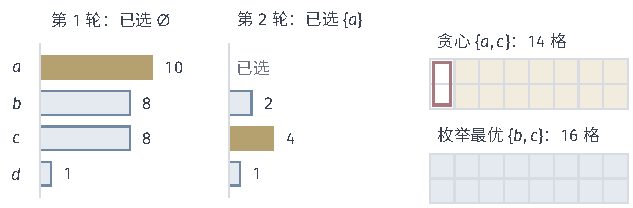
\includegraphics[width=107.177mm]{figures/01-basic-mathematics/04-graphs/tikz/c4-greedy-rounds-vs-optimum/figure.pdf}
  \caption{传感器实例上$k=2$的边际增益贪心。左侧两栏是两轮中各候选元素的当前增益，黄色条为该轮选中的元素；第$2$轮的增益相对于已选的$\{a\}$计算。右侧比较两个覆盖结果：贪心集合$\{a,c\}$（黄色）漏掉第$1$列两格（红框），枚举最优集合$\{b,c\}$（蓝色）覆盖全部$16$格。}
  \label{fig:graph-setfn-greedy-rounds}
\end{figure}

这条轨迹也说明为什么不能只按初始增益排序一次。初始增益的次序是$a$，然后$b,c$并列；按编号取前两个得到$\{a,b\}$，只覆盖$12$格。第$2$轮重新计算后，$b$的增益从$8$降到$2$，$c$的增益从$8$降到$4$，排序已经改变。

\paragraph{求值次数与缓存}
第$t$轮要对$n-t+1$个未选元素各求值一次，总共
\[
  \sum_{t=1}^{k}(n-t+1)\leq nk
\]
次求值，再加上开始时的一次$F(\varnothing)$。传感器实例$n=4$、$k=2$，共$4+3=7$次。若一次求值的代价为$\tau$（例如覆盖量需要合并若干覆盖范围），总代价是$O(nk\tau)$。

对次模函数，可以缓存上一轮算出的增益来减少求值。由式~\eqref{eq:graph-setfn-diminishing-returns}，已选集合变大后，每个元素的增益只会变小，所以旧增益是新增益的上界。每轮把候选元素按缓存值排序，只重新计算排在最前的元素；若它的新增益仍不小于其余元素的缓存值，它就是本轮增益最大者，其余元素不必重算。这种做法的正确性依赖次模性；对一般函数，旧增益不是上界，必须每轮全部重新计算。

\subsection{贪心保证与适用范围}
\label{sec:graph-setfn-greedy-guarantee}

贪心在传感器实例上没有找到最优解，但$14$与$16$相差不多。下面的定理说明这不是巧合：对归一化、单调、次模的目标，贪心值总能达到最优值的一个固定比例。

\begin{theorem}[贪心的近似保证]
\label{thm:graph-setfn-greedy-guarantee}
设$F$是有限底集$V$上的集合函数，满足$F(\varnothing)=0$、单调非减且次模；整数$1\leq k\leq|V|$。记$\mathrm{OPT}$为问题~\eqref{eq:graph-setfn-cardinality-problem}的最优值，$S_\ell$为算法~\ref{alg:graph-setfn-greedy}执行$\ell$轮后的集合（$0\leq\ell\leq k$）。则
\[
  F(S_\ell)\geq\Bigl(1-\bigl(1-\tfrac1k\bigr)^{\ell}\Bigr)\mathrm{OPT}.
\]
特别地，$F(S_k)\geq\bigl(1-(1-1/k)^k\bigr)\mathrm{OPT}\geq(1-e^{-1})\mathrm{OPT}$。
\end{theorem}

\begin{proof}
固定一个最优集合$O$，$|O|\leq k$，$F(O)=\mathrm{OPT}$。考察第$t$轮开始时的集合$S_{t-1}$（$1\leq t\leq k$），先用次模性把它与最优值的差距上界为若干个边际增益之和。把$O\setminus S_{t-1}$中的元素排成$o_1,\ldots,o_r$，由单调性和式~\eqref{eq:graph-setfn-telescoping}，
\[
  \mathrm{OPT}=F(O)\leq F(O\cup S_{t-1})
  =F(S_{t-1})+\sum_{j=1}^{r}\Delta\bigl(o_j\mid S_{t-1}\cup\{o_1,\ldots,o_{j-1}\}\bigr).
\]
每个$o_j$都不在$S_{t-1}\cup\{o_1,\ldots,o_{j-1}\}$中，由式~\eqref{eq:graph-setfn-diminishing-returns}，第$j$项不超过$\Delta(o_j\mid S_{t-1})$。而贪心在第$t$轮选的是增益最大的元素，所以$\Delta(o_j\mid S_{t-1})\leq\Delta(v_t\mid S_{t-1})=F(S_t)-F(S_{t-1})$。又$r\leq|O|\leq k$，且每一项增益非负，于是
\[
  \mathrm{OPT}-F(S_{t-1})\leq k\bigl(F(S_t)-F(S_{t-1})\bigr).
\]
这一步说的是：最优集合至多$k$个元素，它们合起来能补上的差距，至少有$1/k$能被当前最好的单个元素补上。

记差距$\delta_t=\mathrm{OPT}-F(S_t)$。上式可写成$\delta_{t-1}\leq k(\delta_{t-1}-\delta_t)$，即
\[
  \delta_t\leq\Bigl(1-\frac1k\Bigr)\delta_{t-1},\qquad t=1,\ldots,k.
\]
由$F(\varnothing)=0$得$\delta_0=\mathrm{OPT}$，连续使用$\ell$次得$\delta_\ell\leq(1-1/k)^\ell\,\mathrm{OPT}$，移项即为所求。

最后比较$(1-1/k)^k$与$e^{-1}$。函数$\psi(x)=e^{-x}-(1-x)$满足$\psi(0)=0$，导数$\psi'(x)=1-e^{-x}$在$x>0$时为正，所以$\psi$在$[0,+\infty)$上单调递增（第~\ref{sec:ru-monotonicity-convexity}节），从而$0\leq1-x\leq e^{-x}$对$0\leq x\leq1$成立。取$x=1/k$再求$k$次幂，得到$(1-1/k)^k\leq e^{-1}$。
\end{proof}

几个条件各有作用。归一化保证差距从$\mathrm{OPT}$开始；若$F(\varnothing)\neq0$，比例式会因为一个常数而失去意义。单调性用在$F(O)\leq F(O\cup S_{t-1})$和增益非负两处，次模性用在把$O$中元素的增益统一换成相对于$S_{t-1}$的增益。$k=1$时界为$1$，贪心选出的就是最好的单元素；$k=2$时界为$3/4$，传感器实例中$14\geq\frac34\times16=12$，与定理一致。$1-e^{-1}\approx0.632$是对一切$k$都成立的下界。

\paragraph{撤去次模性}
图~\ref{fig:graph-setfn-property-counterexamples}(a)的函数$F(S)=\max\{3\,\mathbb I\{\{1,2\}\subseteq S\},\mathbb I\{3\in S\}\}$单调、归一化，但不是次模的。取$k=2$：第$1$轮三个增益依次为$0,0,1$，选$3$；第$2$轮相对于$\{3\}$，加入$1$或$2$的增益都是$0$，按编号选$1$，得到$F(\{1,3\})=1$。最优集合是$\{1,2\}$，$\mathrm{OPT}=3$。元素$1,2$只有同时选中才有价值，每一轮单独看它们的增益都是零，贪心永远看不到这个互补组合。把$3$换成任意大的$M$，比例$1/M$可以任意小，所以没有次模性就没有固定比例的保证。

\paragraph{撤去单调性}
图~\ref{fig:graph-setfn-property-counterexamples}(b)的单边割权是次模的，但不单调。取$k=2$并按算法~\ref{alg:graph-setfn-greedy}强制选满：第$1$轮选$1$（增益$1$），第$2$轮只剩$2$，增益为$-1$，仍须加入，结果$\operatorname{cut}(\{1,2\})=0$，而至多选两个时的最优值是$1$。在增益为负时停止可以避免这个例子中的损失，但对一般的非单调次模函数，这样修改后的贪心仍没有定理~\ref{thm:graph-setfn-greedy-guarantee}那样的保证，需要另外的算法与分析，本节不展开。

因此，定理~\ref{thm:graph-setfn-greedy-guarantee}只适用于本节规定的问题：在基数约束下最大化归一化、单调、次模的集合函数。它给出的是近似比例，不是精确最优性；目标、约束或函数性质改变时，都需要重新论证。

% 第4章第5节：预算约束下的子集选择（预算约束选择问题；单位成本边际收益法；方法的局限与结果检查）。

\section{预算约束下的子集选择}
\label{sec:graph-budget-selection}

基数约束让每个元素占用一个名额。实际中不同传感器的价格不同，限制的往往是总花费而不是个数。本节说明换成预算约束后，可行集合、选择依据和性能分析各自怎样改变。主线是一种简单可算的逐轮规则，重点放在它的执行过程与失效边界，而不是把上一节的保证直接搬过来。

\subsection{预算约束选择问题}
\label{sec:graph-setfn-budget-problem}

给每个元素$v\in V$指定成本$c_v$，再给定总预算$B\geq0$。要求的是
\begin{equation}
  \max_{S\subseteq V}\ F(S)\qquad\text{满足}\quad\sum_{v\in S}c_v\leq B.
  \label{eq:graph-setfn-budget-problem}
\end{equation}
满足成本条件的子集称为预算可行的，这一条件称为\term{预算约束}（budget constraint）。目标函数$F$与上一节相同，改变的只是允许的子集。所有成本都取$1$、预算取$k$时，预算约束就是基数约束，所以本节的问题是上一节的推广。

成本可能为零的元素需要先单独处理。零成本元素不占预算，若$F$单调，把它们全部加入不会降低目标，可以在开始时一次放进集合；若$F$不单调，它们是否值得加入要看增益的正负。以下设所有成本为正。另外，成本超过$B$的元素不可能出现在任何可行集合中，可以预先删去。

\paragraph{两种约束下的可行集合}
在传感器实例中取成本$c_a=4$、$c_b=3$、$c_c=4$、$c_d=1$，预算$B=7$。预算可行的子集共有$10$个：空集、四个单元素集，以及$\{a,b\}$（成本$7$）、$\{a,d\}$（$5$）、$\{b,c\}$（$7$）、$\{b,d\}$（$4$）、$\{c,d\}$（$5$）；三元及以上的子集成本都超过$7$。枚举得最优集合为$\{b,c\}$，覆盖$16$格。与$k=2$的基数约束相比，$\{a,c\}$成本为$8$，现在不可行了；而$\{a,b\}$在两种约束下都可行。选择的个数不再直接决定资源消耗，每次加入元素前都要检查剩余预算。

\subsection{单位成本边际收益法}
\label{sec:graph-setfn-ratio-greedy}

把上一节的贪心原样搬过来，就是每轮在付得起的元素里选增益最大的。这样做会偏爱昂贵的元素：一个元素增益大，可能只是因为它贵。更合理的比较是每单位成本带来多少增益。

\begin{algorithm}[预算约束下的单位成本贪心]
\label{alg:graph-setfn-ratio-greedy}
输入：有限底集$V$（元素已编号），正成本$c_v$，预算$B\geq0$，单调非减集合函数$F$的求值规则。输出：预算可行的集合。状态：已选集合$S$，剩余预算$R=B-\sum_{v\in S}c_v$，本轮候选元素的增益。
\begin{enumerate}
  \item 令$S=\varnothing$，$R=B$。
  \item 记候选集合$Q=\{v\in V\setminus S:c_v\leq R\}$。若$Q$为空，停止。
  \item 对每个$v\in Q$计算$\Delta(v\mid S)$。若这些增益全为零，停止；否则取比值$\Delta(v\mid S)/c_v$最大的$v$，比值相同时取编号最小者。
  \item 令$S\leftarrow S\cup\{v\}$，$R\leftarrow R-c_v$，回到第2步。
\end{enumerate}
\end{algorithm}

每轮至少加入一个元素，所以算法至多执行$n$轮，求值次数不超过$n+(n-1)+\cdots+1=n(n+1)/2$。停止时有两种原因：没有付得起的元素，或者付得起的元素都不再增加覆盖。

\paragraph{两种规则的对照}
图~\ref{fig:graph-setfn-budget-rule-comparison}在$B=7$的实例上比较“总增益最大”与“单位成本增益最大”两种规则。按总增益，第$1$轮选$a$（增益$10$），剩余预算$3$；第$2$轮付得起的有$b$（增益$2$）和$d$（增益$1$），$c$的成本$4$超出剩余预算，选$b$，剩余预算$0$，停止，覆盖$12$格。按单位成本，第$1$轮的比值为$a:10/4=2.5$，$b:8/3\approx2.67$，$c:8/4=2$，$d:1/1=1$，选$b$，剩余预算$4$；第$2$轮相对于$\{b\}$，$a$的增益为$4$（第$5$、$6$列），比值$1$，$c$的增益为$8$，比值$2$，$d$的增益为$0$，选$c$，剩余预算$0$，停止，覆盖$16$格，恰为枚举最优值。

\begin{figure}[!htb]
  \centering
  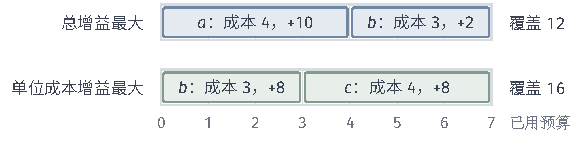
\includegraphics[width=98.538mm]{figures/01-basic-mathematics/04-graphs/tikz/c4-budget-rule-comparison/figure.pdf}
  \caption{预算$B=7$下两种逐轮规则的选择结果（成本$c_a=4$、$c_b=3$、$c_c=4$、$c_d=1$）。每条横条代表$7$个单位的预算，色块的宽度是所选元素的成本，块内写出选择时的增益。按总增益先选昂贵的$a$，剩余预算只够再选增益$2$的$b$，覆盖$12$格；按单位成本先选$b$，再选$c$，覆盖$16$格。}
  \label{fig:graph-setfn-budget-rule-comparison}
\end{figure}

\paragraph{与最佳单元素比较}
单位成本规则也有自己的偏差：它可能先选几个便宜的小元素，把预算切碎，使一个昂贵但价值很高的元素再也放不进去。一种简单的补救是在算法结束后，再计算每个可行单元素的值$F(\{v\})$（$c_v\leq B$），输出$S$与最佳单元素中函数值较大的一个。这只需另外$n$次求值。在$B=7$的实例中，最佳单元素是$\{a\}$，覆盖$10$格，小于$16$，输出仍是$\{b,c\}$。这一检查只是一个具体策略；本节没有给出它的分析，因此不附加一般的近似比例。

\subsection{方法的局限与结果检查}
\label{sec:graph-setfn-budget-limits}

单位成本规则在上面的实例中表现很好，但下面的例子说明它本身没有任何固定比例的保证。

\begin{example}[比值规则的失效]
\label{ex:graph-setfn-ratio-failure}
底集$\{u,w\}$，预算$B=100$。$u$的成本为$1$、价值为$2$，$w$的成本为$100$、价值为$100$，目标取模函数$F(S)=\sum_{v\in S}(\text{价值})$。它单调，也是次模的。

比值规则第$1$轮比较$2/1=2$与$100/100=1$，选$u$；剩余预算$99<100$，$w$付不起，算法停止，得$F(\{u\})=2$。最优选择是$\{w\}$，$F=100$。见图~\ref{fig:graph-setfn-budget-ratio-failure}。把$w$的成本、价值与预算同时换成任意大的$M$，比值规则仍先选$u$，得到$2$而最优值为$M$，比例$2/M$可以任意小。
\end{example}

\begin{figure}[!htb]
  \centering
  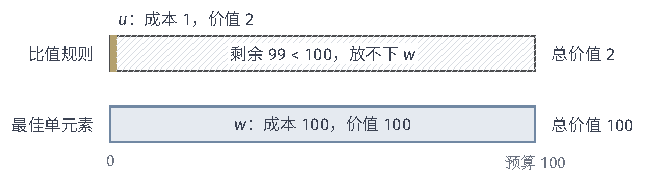
\includegraphics[width=109.146mm]{figures/01-basic-mathematics/04-graphs/tikz/c4-budget-ratio-failure/figure.pdf}
  \caption{比值规则的失效例。横条长度代表预算$100$。上行：比值规则先选单位价值较高的$u$（黄色，成本$1$，为便于观察略加宽），剩余$99$个单位（斜线）放不下成本$100$的$w$，总价值$2$。下行：最佳单元素$w$恰好用满预算，总价值$100$。}
  \label{fig:graph-setfn-budget-ratio-failure}
\end{figure}

这个例子的目标是模函数，从而单调且次模，可见即使目标满足上一节定理的全部函数条件，原始比值规则也不能继承那里的保证：预算约束改变了可行集合的结构，证明中“最优集合至多$k$个元素”这一步不再有对应物。上一小节的最佳单元素比较能修复这个例子，因为它会发现$\{w\}$；但修复一个例子不构成一般保证。具有严格保证的预算选择算法需要另外的枚举或修正机制，并要给出相应的证明，本书不展开，也不应把它们与这里的简单规则混为一谈。

\paragraph{结果检查}
小实例可以直接枚举全部预算可行子集，核对三件事：输出集合的总成本不超过预算，输出的函数值计算无误，以及它与枚举最优值的差距。上面$B=7$的实例只有$10$个可行子集，比值规则的结果$\{b,c\}$与枚举最优一致，总增益规则的结果$\{a,b\}$差$4$格。大实例无法枚举时，至少应报告所用预算与剩余预算、最终目标值、最佳单元素的值，以及总求值次数和每次求值的代价。最佳单元素给出一个必须超过的基准；若逐轮规则的结果不如它，往往就是出现了示例~\ref{ex:graph-setfn-ratio-failure}那样预算被小元素切碎的情形。

% 第4章第6节：成对二值函数的最小化（成对二值最小化问题；次模条件与割表示；最小割求解与解的恢复）。

\section{成对二值函数的最小化}
\label{sec:graph-pairwise-binary-cut}

前两节在约束下最大化一般的集合函数，只能得到近似解。本节换一个方向：目标是最小化，没有基数或预算约束，但函数具有特殊的结构，即由只涉及单个元素的一元项和只涉及两个元素的成对项相加而成。利用子集与二值向量的对应，我们把这样的目标在一定条件下表示为割的容量，再调用第~\ref{sec:graph-max-flow}节的最小割，求出精确的最优解。

\subsection{成对二值最小化问题}
\label{sec:graph-setfn-pairwise-problem}

给底集$V$的每个元素$i$一个二值变量$x_i\in\{0,1\}$，$x_i=1$表示选中$i$，于是配置$\bm x\in\{0,1\}^V$就是第~\ref{sec:graph-setfn-binary-vectors}节的指示向量。元素之间的交互用无向图$\mathcal G=(V,E)$记录：只有$\{i,j\}\in E$的两个元素之间有成对项。目标是
\begin{equation}
  \min_{\bm x\in\{0,1\}^V}J(\bm x),\qquad
  J(\bm x)=\sum_{i\in V}\phi_i(x_i)+\sum_{\{i,j\}\in E}\phi_{i,j}(x_i,x_j).
  \label{eq:graph-setfn-pairwise-objective}
\end{equation}
\term{一元项}$\phi_i$给出元素$i$两种状态各自的成本，只有两个数$\phi_i(0),\phi_i(1)$；\term{成对项}$\phi_{i,j}$给出$i,j$四种联合状态的成本，例如两者取值不同时的不一致代价，或两者同时选中的配合收益（以负成本表示）。为了让$\phi_{i,j}(a,b)$的含义确定，对每条边固定一个次序，约定$a$是$x_i$、$b$是$x_j$的值。本节只考虑有限实值成本。

通过$S=\{i:x_i=1\}$，$J$也是$V$上的集合函数。但并不是每个集合函数都能写成式~\eqref{eq:graph-setfn-pairwise-objective}的形式：例如只在三个元素同时选中时才产生的成本，不能拆成两两之间的成对项。本节的方法只适用于已经具有这种一元加成对结构的目标。

\paragraph{逐点选择为什么不够}
取两个变量，$\phi_1(0)=0$、$\phi_1(1)=1$，$\phi_2(0)=2$、$\phi_2(1)=0$，成对项为
\[
  \phi_{1,2}(0,0)=0,\quad\phi_{1,2}(0,1)=3,\quad\phi_{1,2}(1,0)=5,\quad\phi_{1,2}(1,1)=0.
\]
图~\ref{fig:graph-setfn-pairwise-config-table}列出四种配置的成本。若只看一元项，元素$1$偏好$0$，元素$2$偏好$1$，逐点选择得到$(0,1)$，成本$0+0+3=3$。但成对项惩罚两者取值不同，整体最优是$(1,1)$，成本$1+0+0=1$：让元素$1$放弃自己的偏好只多付$1$，却省下了$3$的不一致代价。

\begin{figure}[!htb]
  \centering
  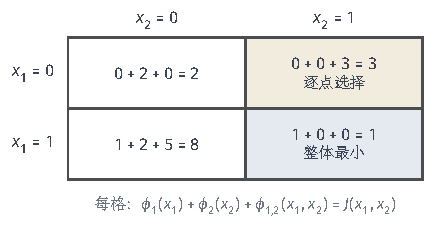
\includegraphics[width=72.383mm]{figures/01-basic-mathematics/04-graphs/tikz/c4-pairwise-config-table/figure.pdf}
  \caption{两变量成对二值函数的四种配置。行是$x_1$，列是$x_2$，每格依次写出$\phi_1(x_1)$、$\phi_2(x_2)$、$\phi_{1,2}(x_1,x_2)$与总成本$J$。逐点按一元项选择得到黄色格$(0,1)$，成本$3$；整体最小是蓝色格$(1,1)$，成本$1$。}
  \label{fig:graph-setfn-pairwise-config-table}
\end{figure}

两个变量可以枚举，$n$个变量则有$2^n$种配置。下面把四种配置的成本同时编码进一个网络的割容量，使枚举变成一次最小割计算。

\subsection{次模条件与割表示}
\label{sec:graph-setfn-cut-representation}

割容量只能累加非负的弧容量，因此能否编码取决于成对项的形状。关键条件是对每条边$\{i,j\}\in E$成立
\begin{equation}
  \phi_{i,j}(0,0)+\phi_{i,j}(1,1)\leq\phi_{i,j}(0,1)+\phi_{i,j}(1,0).
  \label{eq:graph-setfn-pairwise-submodular}
\end{equation}
它正是两元素底集$\{i,j\}$上的次模不等式：把$\phi_{i,j}$看成$\{i,j\}$上的集合函数，在式~\eqref{eq:graph-setfn-submodular-inequality}中取$X=\{i\}$、$Y=\{j\}$，左边$F(X)+F(Y)$对应$\phi_{i,j}(1,0)+\phi_{i,j}(0,1)$，右边$F(X\cup Y)+F(X\cap Y)$对应$\phi_{i,j}(1,1)+\phi_{i,j}(0,0)$。一元项是模函数，若每个成对项都满足式~\eqref{eq:graph-setfn-pairwise-submodular}，则$J$作为集合函数是次模的。上面的例子中$0+0\leq3+5$，条件成立。

\paragraph{成对项的分解}
条件~\eqref{eq:graph-setfn-pairwise-submodular}允许把一个成对项拆成常数、两个一元的线性部分和一个非负的不一致惩罚。

\begin{lemma}[成对项的分解]
\label{lem:graph-setfn-pairwise-decomposition}
设$\phi_{i,j}$满足式~\eqref{eq:graph-setfn-pairwise-submodular}，简记$p_{a,b}=\phi_{i,j}(a,b)$，令
\[
  \begin{gathered}
  w_{i,j}=\frac{p_{0,1}+p_{1,0}-p_{0,0}-p_{1,1}}{2},\\
  \alpha_i=p_{1,0}-p_{0,0}-w_{i,j},\qquad
  \alpha_j=p_{0,1}-p_{0,0}-w_{i,j}.
  \end{gathered}
\]
则$w_{i,j}\geq0$，并且对四种配置都有
\begin{equation}
  \phi_{i,j}(x_i,x_j)=p_{0,0}+\alpha_ix_i+\alpha_jx_j+w_{i,j}\,|x_i-x_j|.
  \label{eq:graph-setfn-pairwise-decomposition}
\end{equation}
\end{lemma}

\begin{proof}
$w_{i,j}\geq0$就是式~\eqref{eq:graph-setfn-pairwise-submodular}移项除以$2$。逐个代入四种配置核对右边：$(0,0)$时为$p_{0,0}$；$(1,0)$时为$p_{0,0}+\alpha_i+w_{i,j}=p_{1,0}$；$(0,1)$时为$p_{0,0}+\alpha_j+w_{i,j}=p_{0,1}$；$(1,1)$时为$p_{0,0}+\alpha_i+\alpha_j=p_{1,0}+p_{0,1}-p_{0,0}-2w_{i,j}=p_{1,1}$，最后一步代入$w_{i,j}$的定义。
\end{proof}

在例子中，$w_{1,2}=(3+5-0-0)/2=4$，$\alpha_1=5-0-4=1$，$\alpha_2=3-0-4=-1$。

\paragraph{一元项的合并与移位}
对每条边作上述分解，把常数$\phi_{i,j}(0,0)$累加起来，把线性部分$\alpha_ix_i$、$\alpha_jx_j$并入相应元素的一元项。记合并后的一元项为$\psi_i$，即$\psi_i(0)=\phi_i(0)$，$\psi_i(1)=\phi_i(1)$加上与$i$关联的各边分解出的$\alpha_i$。$\psi_i$可能取负值，而容量必须非负，所以再令$m_i=\min\{\psi_i(0),\psi_i(1)\}$，$\tilde\psi_i=\psi_i-m_i$，两种状态的成本都减去同一个数，$\tilde\psi_i$的两个值非负且至少一个为零。移出的数另行累计成常数
\[
  K=\sum_{\{i,j\}\in E}\phi_{i,j}(0,0)+\sum_{i\in V}m_i .
\]
于是对每个配置都有
\begin{equation}
  J(\bm x)=K+\sum_{i\in V}\tilde\psi_i(x_i)+\sum_{\{i,j\}\in E}w_{i,j}\,|x_i-x_j|,
  \label{eq:graph-setfn-shifted-objective}
\end{equation}
右边除常数$K$外各项都非负。在例子中，$\psi_1=(0,\,1+1)=(0,2)$，$\psi_2=(2,\,0-1)=(2,-1)$；$m_1=0$，$m_2=-1$，所以$\tilde\psi_1=(0,2)$，$\tilde\psi_2=(3,0)$，$K=0+0+(-1)=-1$。

\paragraph{网络构造}
由式~\eqref{eq:graph-setfn-shifted-objective}构造有向网络：顶点为$V\cup\{s,t\}$；对每个$i\in V$，建弧$s\to i$，容量$\tilde\psi_i(1)$，以及弧$i\to t$，容量$\tilde\psi_i(0)$；对每条边$\{i,j\}\in E$，建方向相反的两条弧$i\to j$与$j\to i$，容量都是$w_{i,j}$。容量为零的弧可以省略。规定源侧的元素取$0$、汇侧的元素取$1$，即配置$\bm x$对应$s$--$t$割$(S_{\bm x},\bar S_{\bm x})$，其中$S_{\bm x}=\{s\}\cup\{i:x_i=0\}$。用最小割求解这类问题的方法常称为\term{图割}（graph cut）。

\begin{theorem}[成对二值函数的割表示]
\label{thm:graph-setfn-cut-representation}
设式~\eqref{eq:graph-setfn-pairwise-objective}中的成本都是有限实数，且每个成对项满足式~\eqref{eq:graph-setfn-pairwise-submodular}。则在上面构造的网络中，配置与$s$--$t$割一一对应，并且每个配置$\bm x$对应的割容量等于$J(\bm x)-K$。因此最小割对应的配置是$J$的最小点。
\end{theorem}

\begin{proof}
任一$s$--$t$割的源侧都含$s$、不含$t$，由$V$中哪些元素在源侧唯一确定，所以割与配置一一对应。割容量只累计从源侧指向汇侧的弧，逐类计算。若$x_i=0$，$i$在源侧，弧$i\to t$跨出，计入$\tilde\psi_i(0)$，弧$s\to i$两端都在源侧，不计入；若$x_i=1$，$i$在汇侧，弧$s\to i$跨出，计入$\tilde\psi_i(1)$，弧$i\to t$两端都在汇侧，不计入。两种情形合起来恰好计入$\tilde\psi_i(x_i)$。对边$\{i,j\}$，若$x_i=x_j$，两条弧都不跨越；若$x_i\neq x_j$，两条反向弧中恰有一条从源侧指向汇侧，计入一次$w_{i,j}$。合起来恰好计入$w_{i,j}|x_i-x_j|$。所以割容量等于式~\eqref{eq:graph-setfn-shifted-objective}右边去掉$K$，即$J(\bm x)-K$。$K$与配置无关，最小化割容量与最小化$J$是同一件事。
\end{proof}

在例子中，网络有弧$s\to1$（容量$2$）、$2\to t$（容量$3$）、$1\to2$与$2\to1$（容量都是$4$），弧$1\to t$与$s\to2$容量为零。表~\ref{tab:graph-setfn-cut-check}逐个核对四种配置：割容量都比$J$大$1$，即$-K$。

\begin{table}[!htb]
  \centering
  \begin{tabular}{cccc}
    \toprule
    配置$\bm x$ & 源侧 & 跨出的正容量弧 & 割容量 / $J(\bm x)$ \\
    \midrule
    $(0,0)$ & $\{s,1,2\}$ & $2\to t$ & $3$ / $2$ \\
    $(0,1)$ & $\{s,1\}$ & $1\to2$ & $4$ / $3$ \\
    $(1,0)$ & $\{s,2\}$ & $s\to1$，$2\to t$，$2\to1$ & $9$ / $8$ \\
    $(1,1)$ & $\{s\}$ & $s\to1$ & $2$ / $1$ \\
    \bottomrule
  \end{tabular}
  \caption{两变量例子中四种配置的割容量与原目标值。源侧元素取$0$、汇侧元素取$1$；每行割容量都等于$J(\bm x)+1$，相差的常数是$-K=1$，所以割容量最小的$(1,1)$也是$J$的最小点。}
  \label{tab:graph-setfn-cut-check}
\end{table}

\paragraph{条件不成立时}
若某个成对项违反式~\eqref{eq:graph-setfn-pairwise-submodular}，引理给出的$w_{i,j}$为负，网络中就会出现负容量的弧。第~\ref{sec:graph-max-flow}节的流值与割容量的关系建立在非负容量之上，负容量时不能直接使用。例如奖励两个变量取值不同的成对项$\phi_{i,j}(0,1)=\phi_{i,j}(1,0)=0$、$\phi_{i,j}(0,0)=\phi_{i,j}(1,1)=1$就违反条件，这时的最小化一般不能化为一次最小割。

\subsection{最小割求解与解的恢复}
\label{sec:graph-setfn-cut-solving}

\paragraph{求解步骤}
构造网络后，用第~\ref{sec:graph-max-flow}节的Edmonds--Karp算法求最大流。算法停止时，残量网络中从$s$可达的顶点集合是一个最小割的源侧；把其中的元素标为$0$，其余元素标为$1$，就得到最优配置$\hat{\bm x}$。结果可以独立核对：直接按式~\eqref{eq:graph-setfn-pairwise-objective}计算$J(\hat{\bm x})$，它应等于最大流值加$K$。由于最大流值等于最小割容量，这个等式同时证明了$\hat{\bm x}$的最优性，而不必相信算法实现本身。

\paragraph{两变量例子的求解}
网络中从$s$到$t$只有一条正容量路径$s\to1\to2\to t$，瓶颈为$\min\{2,4,3\}=2$。沿它增广$2$个单位后，$s\to1$的正向残量为零，$s\to2$本来容量为零，所以残量网络中从$s$出发哪里也到不了，可达集合是$\{s\}$。最小割容量$2$等于流值，两个元素都在汇侧，得到$\hat{\bm x}=(1,1)$。代回原目标，$J(1,1)=1+0+0=1=2+K$，与图~\ref{fig:graph-setfn-pairwise-config-table}中的枚举结果一致。图~\ref{fig:graph-setfn-st-cut-construction}把这个最小割与配置$(0,1)$对应的割并排比较。

\begin{figure}[!htb]
  \centering
  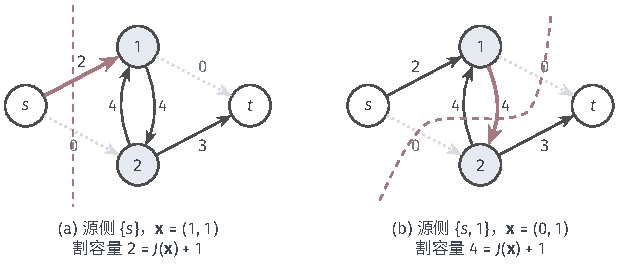
\includegraphics[width=104.687mm]{figures/01-basic-mathematics/04-graphs/tikz/c4-st-cut-construction/figure.pdf}
  \caption{两变量例子的$s$--$t$网络。弧旁数字是容量，灰色点线是容量为零的弧；红色虚线分开源侧与汇侧，红色粗弧是跨出割的正容量弧。源侧元素取$0$、汇侧元素取$1$。(a) 最小割，源侧$\{s\}$，只割断$s\to1$，容量$2$，对应$(1,1)$；(b) 源侧$\{s,1\}$，割断$1\to2$，容量$4$，对应逐点选择得到的$(0,1)$。两种情况的割容量都等于$J(\bm x)+1$。}
  \label{fig:graph-setfn-st-cut-construction}
\end{figure}

\paragraph{开销}
网络有$n+2$个顶点，弧数$a\leq2n+2m$，其中$m=|E|$；计算分解、合并一元项和建弧都只需扫描一遍元素与边，用时$O(n+m)$。主要开销在最大流：按第~\ref{sec:graph-max-flow}节的分析，Edmonds--Karp算法需要$O(na^2)$次算术与比较操作，代入$a=O(n+m)$即$O(n(n+m)^2)$。与枚举$2^n$种配置相比，这是多项式规模的计算。

\paragraph{与前两节的比较}
本节与前两节都在子集上做选择，但条件和结论不同。前两节在基数或预算约束下最大化单调次模函数，得到的是近似解，保证依赖单调性、次模性和约束的形式。本节最小化可以写成一元项加满足式~\eqref{eq:graph-setfn-pairwise-submodular}的成对项的函数，没有额外约束，得到的是精确解，依据是割表示。在本节的问题上再加“恰好选$k$个”这样的数量限制，割与配置的对应就不再保持约束；含三个及以上变量的高阶项、违反条件的成对项，以及每个变量有三种以上取值的问题，也都不能直接套用这个构造。一般次模函数的最小化另有专门的算法，超出本书范围。

% 第4章第7节：本章小结。

\section{本章小结}
\label{sec:graph-set-functions-summary}

本章从传感器覆盖出发，把对整组选择的评价写成有限底集上的集合函数。元素之间若互不影响，每个元素贡献一个固定的数，集合函数就是模函数；覆盖范围的重叠使边际增益随已选集合增大而递减，这就是次模性；部件之间的协同则产生相反方向的超模性。单调、模、次模各自约束不同的东西，覆盖量、割权和净收益说明它们可以以各种方式组合，判断时要回到边际增益或四个函数值的不等式逐项核对。子集累计与Möbius反演完成的是另一项任务：已知全部子集的累计值，按元素个数之差交替加减，恢复每个子集自身的贡献；它只依赖有限求和与包含关系，结果可以为负，计算开销随底集大小指数增长。

选择问题按目标方向与约束分别处理。在基数约束下最大化归一化、单调、次模的函数，逐轮加入当前增益最大的元素，所得值不低于最优值的$1-(1-1/k)^k$倍；撤去次模性，贪心会错过互补组合，撤去单调性，强制选满会降低目标。换成预算约束后，单位成本规则在传感器实例中找到了最优解，但在成本为$(1,2)$与$(100,100)$的例子中可以任意差，最佳单元素比较只修复个别失效。最小化由一元项和满足次模条件的成对项组成的函数时，目标可以表示为$s$--$t$网络的割容量，一次最小割给出精确解，并附带可以独立核对的证书。使用任何一种方法之前，都要同时写明目标方向、约束、单调性、次模性以及函数的表示结构。

第~\ref{sec:graph-pairwise-binary-cut}节的成功依赖两点：每个变量只有两种状态，成对项满足特定的不等式。许多问题两点都不满足，变量可以有更多取值，局部成本可以同时读取三个变量，或者直接禁止某些组合；但整体函数常常仍是许多局部项之和，每一项只读取少数变量。第~\ref{chap:graph-dynamic-programming}章从这里出发，研究怎样借助记录局部项读取关系的依赖图，把对全部配置的枚举化为沿图逐步传递的小规模表格计算。


\chapter{图上的动态规划}
\label{chap:graph-dynamic-programming}

第~\ref{sec:graph-pairwise-binary-cut}节把每个顶点的“选或不选”写成二值变量，并在成对成本满足特定条件时用最小割求出整体最优。许多问题并不满足那里的条件：变量可以有三种以上的取值，局部成本也可以同时读取三个变量，还可能直接禁止某些组合。不过它们常常保留另一种结构：整体成本是许多局部项之和，每一项只读取少数几个变量。本章研究怎样利用这种局部依赖，求出有限状态配置的最小成本和最优配置，并顺带得到可行配置的个数与有限加权总量。

直接枚举全部配置的开销随变量数指数增长，所以关键在于把已经处理过的变量压缩起来。第~\ref{sec:graph-local-functions}节先说明问题由什么组成：变量的有限状态、只读取少数变量的局部函数，以及记录这些读取关系的几种图。第~\ref{sec:graph-tree-dp}节在链和树上建立基本做法：固定已处理部分与其余部分之间的接口变量，把已处理部分的最小成本记成一张接口表，再把接口表逐步传向根，最后沿保存的选择回溯出配置。

一般依赖图上没有天然的“从叶到根”次序。第~\ref{sec:graph-variable-elimination}节把端点汇总推广为逐个消去变量，证明任意次序都给出正确结果，但中间表的大小随次序变化。为了描述消元时需要同时处理哪些变量，第~\ref{sec:graph-tree-decomposition}节引入树分解，把变量组织成一棵由“袋”组成的树，并用树宽刻画袋的大小；第~\ref{sec:graph-tree-decomposition-construction}节说明怎样由消元次序构造树分解，怎样选择次序，以及在弦图上怎样用极大团和第~\ref{sec:graph-minimum-spanning-tree}节的最大权生成树得到团树。第~\ref{sec:graph-bag-dp}节回到数值计算，把树上的接口递推搬到袋组成的树上，并把最小成本换成计数和加权求和。

% 第5章第1节：局部函数与图表示（有限状态与配置、局部函数与作用域、依赖图、因子图、原始关系图与超图）。

\section{局部函数与图表示}
\label{sec:graph-local-functions}

本章的问题都从一组变量的联合取值出发：每个变量从有限个状态中取一个，整组取值按某种规则得到成本，或者被判为不允许。描述这样的问题需要两类信息。一类是数值：每个局部规则对每种取值给出多少成本；另一类是结构：哪些变量出现在同一条规则里。本节先把这两类信息分开，再说明几种图分别保存了哪些结构信息。后面的计算方法都以这里的区分为前提，图记录读取关系，局部函数表记录具体数值，二者不能互相替代。

\subsection{有限状态与配置}

考虑三台相邻的设备，每台可以关（记为$0$）或开（记为$1$）。用$x_1,x_2,x_3$分别表示三台设备的状态，一次联合取值$(x_1,x_2,x_3)$就确定了全部设备的状态。三台设备共有$2^3=8$种联合取值：
\[
(0,0,0),\ (0,0,1),\ (0,1,0),\ (0,1,1),\ (1,0,0),\ (1,0,1),\ (1,1,0),\ (1,1,1).
\]
一般地，设变量的下标集合为$V=\{1,\ldots,n\}$，给每个变量$x_i$指定一个非空有限的\term{状态集合}$\mathcal X_i$。全部变量的一次联合取值$\bm x=(x_1,\ldots,x_n)$称为一个\term{配置}（configuration），全部配置组成笛卡尔积
\[
\mathcal X=\prod_{i\in V}\mathcal X_i .
\]
对下标子集$S\subseteq V$，记$\bm x_S$为配置在$S$上的部分，即只保留$S$中下标的那些分量。

配置的数目是$|\mathcal X|=\prod_{i\in V}|\mathcal X_i|$。若每个变量至多有$q$个状态，配置数可以达到$q^n$。三台设备时只有$8$种，三十个二值变量就已超过十亿种。直接逐个计算每种配置的成本再比较，开销随$n$指数增长；本章各节的目的，就是在成本具有局部结构时避开这种枚举。

这里需要区分两种函数。给每个顶点单独赋一个数的函数，每个值只对应一个位置，第~\ref{chap:graph-spectral}章将研究这类顶点函数；本章关心的是给整组配置赋值的函数$F:\mathcal X\to\mathbb R\cup\{+\infty\}$，它的一次求值要读入全部变量的状态。二值情形下，配置$\bm x\in\{0,1\}^n$与子集$\{i:x_i=1\}$一一对应，所以第~\ref{sec:graph-set-function-basics}节的集合函数也可以看成二值配置的函数。一般有限状态则允许每个变量有多种标签，例如三档取值$\{0,1,2\}$。这种对应只是换了一种表示，并不意味着任意整体函数都容易求最小值；能否高效计算，取决于下面要讨论的局部结构。

\subsection{局部函数与作用域}

回到三台设备。假设相邻两台设备状态不同时会产生$1$个单位的切换成本，状态相同时没有成本。设备$1,2$之间的成本只取决于$x_1,x_2$，设备$2,3$之间的成本只取决于$x_2,x_3$，于是总成本可以写成
\[
F(x_1,x_2,x_3)=\phi_{1,2}(x_1,x_2)+\phi_{2,3}(x_2,x_3),\qquad
\phi_{i,j}(a,b)=\begin{cases}0,&a=b,\\1,&a\neq b.\end{cases}
\]
图~\ref{fig:graph-dp-configuration-scopes}左侧列出了全部$8$种配置及其总成本：$(0,0,0)$和$(1,1,1)$成本为$0$，$(0,1,0)$和$(1,0,1)$成本为$2$，其余为$1$。右侧显示，计算任何一个配置的总成本时，$\phi_{1,2}$从不需要看$x_3$，$\phi_{2,3}$也从不需要看$x_1$。

\begin{figure}[!htb]
  \centering
  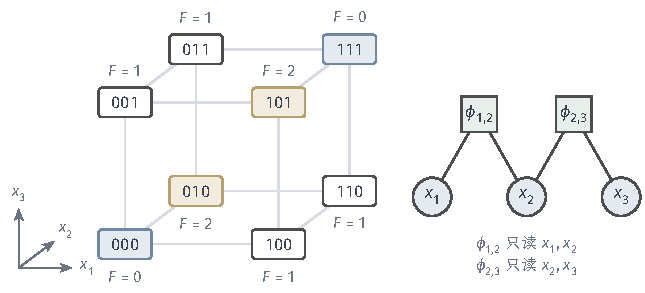
\includegraphics[width=109.269mm]{figures/01-basic-mathematics/04-graphs/tikz/c5-configuration-scopes/figure.pdf}
  \caption{配置空间与局部作用域。左：三个二值变量的$8$种配置排在立方体的顶点上，顶点旁的数是总成本$F=\phi_{1,2}+\phi_{2,3}$，其中相邻变量取值不同时成本为$1$；蓝色顶点成本为$0$，黄色顶点成本为$2$。右：圆点表示变量，方块表示局部函数，连线表示该函数读取的变量。每个局部函数只读取两个变量，但它们的和仍然对全部$8$种配置给出成本。}
  \label{fig:graph-dp-configuration-scopes}
\end{figure}

把这个例子一般化，设有一组局部项，用下标$a\in A$区分。每一项$\phi_a$只读取下标集合$S_a\subseteq V$中的变量，总成本为
\begin{equation}
F(\bm x)=\sum_{a\in A}\phi_a(\bm x_{S_a}),\qquad \bm x\in\mathcal X .
\label{eq:graph-dp-local-sum}
\end{equation}
这里的$\phi_a$称为\term{局部函数}（local function），也常称为\term{因子}（factor）；它读取的下标集合$S_a$称为$\phi_a$的\term{作用域}（scope）。“局部”限定的是读取范围：$\phi_a$精确地给出$\bm x_{S_a}$每种取值的成本，并不是对某个整体函数的近似；作用域也不限于两个变量，三元、四元的局部函数同样允许。一元项$\phi_i(x_i)$是作用域为$\{i\}$的特例。

局部函数的取值允许为$+\infty$，用来表示禁止的组合。例如设备$1,2$不能同时打开时，可以令$\phi_{1,2}(1,1)=+\infty$。约定$+\infty$加任何有限数或$+\infty$仍得$+\infty$，于是只要某一项禁止，整个配置的总成本就是$+\infty$。总成本有限的配置称为\term{可行配置}。这样，同一个式~\eqref{eq:graph-dp-local-sum}既表达偏好，也表达约束；求最小值时还要同时回答是否存在可行配置：最小值为$+\infty$，就说明所有配置都被某项禁止。

式~\eqref{eq:graph-dp-local-sum}是问题给出的分解，不是自动成立的性质。任意函数$F$都可以写成作用域为$V$的单个“局部”函数，但这时局部函数表就有$|\mathcal X|$项，与直接枚举没有区别。本章始终假定分解已经由问题给出，并且各作用域都较小；从一个任意给定的整体函数中寻找小作用域分解，是另一个问题。

\subsection{依赖图与因子图}

只有成对局部项时，可以用一个图记录哪些变量出现在同一项里：以变量为顶点，两个变量出现在同一个成对项中就连一条边。三台设备的例子得到路径$1-2-3$。这样的图记录的是函数的依赖关系，不是变量的取值本身；称“依赖结构是一条链”或“是一棵树”，指的就是这个图是路径或树。

三元及更高阶的局部项无法用一条边表示。这时把变量和局部函数分成两类节点：每个变量一个圆形节点，每个局部函数一个方形节点；变量属于某个局部函数的作用域时，在两者之间连边。这样得到的二部图称为\term{因子图}（factor graph）。因子图保留了每个局部函数的身份：两个不同的局部函数即使作用域相同，也是两个不同的方形节点。图~\ref{fig:graph-dp-configuration-scopes}右侧就是三台设备例子的因子图。

\paragraph{三种表示的对照}
考虑四个二值变量和两个三元局部函数，作用域分别为$S_A=\{1,2,3\}$和$S_B=\{2,3,4\}$。除因子图外，还有两种常用的结构表示。一种不保留函数节点，把每个作用域内的变量两两连边，得到的图称为\term{原始关系图}（primal graph），简称原始图。这里原始图有边$\{1,2\},\allowbreak\{1,3\},\allowbreak\{2,3\},\allowbreak\{2,4\},\allowbreak\{3,4\}$，唯独缺少$\{1,4\}$，因为变量$1$和$4$从不出现在同一个局部函数中。另一种允许一条“边”包含任意多个顶点：每个作用域记为一条\term{超边}（hyperedge），由此得到\term{超图}（hypergraph）。这里超图有两条超边$\{1,2,3\}$和$\{2,3,4\}$。图~\ref{fig:graph-dp-three-representations}并排画出了三种表示。

\begin{figure}[!htb]
  \centering
  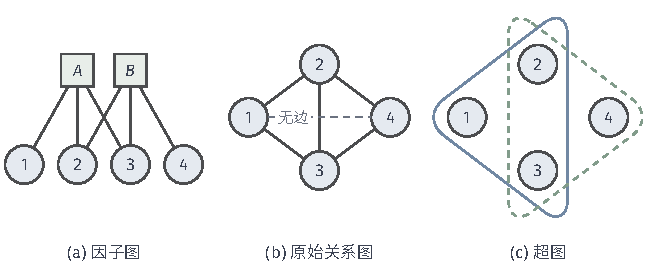
\includegraphics[width=111.936mm]{figures/01-basic-mathematics/04-graphs/tikz/c5-three-representations/figure.pdf}
  \caption{作用域$\{1,2,3\}$与$\{2,3,4\}$的三种结构表示。左：因子图，方块$A$、$B$是两个局部函数，连线表示读取关系。中：原始关系图，把每个作用域内的变量两两相连，只缺边$\{1,4\}$。右：超图，蓝色实线与绿色虚线围出的区域各是一条超边。若把两个三元函数换成五条边上的五个成对函数，原始图完全相同，而因子图和超图都会改变。}
  \label{fig:graph-dp-three-representations}
\end{figure}

原始图丢失了作用域的分组。若把$\phi_A,\phi_B$换成定义在五条边上的五个成对局部函数，原始图不变，因子图和超图却不同。更重要的是，相同的两两连接不能恢复函数表。设$\phi_A(x_1,x_2,x_3)$在$x_1+x_2+x_3$为偶数时取$0$、为奇数时取$+\infty$，$\phi_B$对$x_2+x_3+x_4$作同样的规定。$\phi_A$允许的取值恰为$(0,0,0),(0,1,1),(1,0,1),(1,1,0)$，其中任意两个变量的四种取值组合都出现过。因此，若只保留“每对变量允许哪些取值”的成对规则，这些规则什么也不禁止，$16$种配置都会被放行；而原问题中$x_2,x_3$确定后$x_1,x_4$都被唯一确定，只有$4$种可行配置。

超图保住了作用域的分组，但和原始图一样不保存局部函数的数值；因子图保住了函数身份，但仍需另外存储每个函数的取值表。后面的树分解以原始图为结构依据，因为原始图上的边已经足以说明哪些变量必须同时出现；计算时则始终使用完整的局部函数，不把它们拆成成对规则。

% 第5章第2节：链与树上的动态规划（链上的接口表递推、树上的消息与后序、最优配置的回溯）。

\section{链与树上的动态规划}
\label{sec:graph-tree-dp}

本节只考虑一元项和成对项，并假定成对项组成的依赖图没有环。这时总成本为
\begin{equation}
F(\bm x)=\sum_{i\in V}\phi_i(x_i)+\sum_{\{u,v\}\in E}\phi_{u,v}(x_u,x_v),
\label{eq:graph-dp-pairwise-cost}
\end{equation}
其中$\mathcal G=(V,E)$是依赖图，$\phi_{u,v}(x_u,x_v)$与$\phi_{v,u}(x_v,x_u)$指同一个局部函数。没有一元项的变量可以取$\phi_i\equiv0$。本节从链开始，说明怎样把已经处理过的变量压缩成一张只依赖接口变量的表；再把单个前驱推广为多个子树，得到树上的消息；最后说明怎样从这些表中恢复一个最优配置。依赖图带环、或者局部函数读取三个以上变量的情形，留到下一节。

\subsection{链上的递推}

\paragraph{固定接口变量}
先看三个变量的链$1-2-3$，每个变量取三档$\{0,1,2\}$，总成本$F=\phi_{1,2}(x_1,x_2)+\phi_{2,3}(x_2,x_3)$。两张局部函数表按行列给出：
\[
\bigl[\phi_{1,2}(x_1,x_2)\bigr]=\begin{bmatrix}4&1&3\\2&3&5\\3&4&2\end{bmatrix},\qquad
\bigl[\phi_{2,3}(x_2,x_3)\bigr]=\begin{bmatrix}1&3&2\\4&3&5\\2&2&4\end{bmatrix},
\]
左表的行对应$x_1=0,1,2$、列对应$x_2=0,1,2$，右表的行对应$x_2$、列对应$x_3$。直接枚举要计算$3^3=27$个配置的成本。

注意$x_1$只出现在$\phi_{1,2}$中。若先把$x_2$固定为某个值，$x_1$的选择就不再影响$\phi_{2,3}$，只需在左表的这一列中取最小。对$x_2=0,1,2$分别取列最小值，得到一张只依赖$x_2$的表
\[
m_{1\to2}(x_2)=\min_{x_1}\phi_{1,2}(x_1,x_2)=(2,\,1,\,2),
\]
达到最小值的$x_1$依次为$1,0,2$。这张表概括了链左端的全部信息：无论右侧怎样取值，只要$x_2$给定，左端最好的做法和它的成本都已确定。接下来只需在$x_2,x_3$上求
\[
\min_{x_2,x_3}\bigl[m_{1\to2}(x_2)+\phi_{2,3}(x_2,x_3)\bigr].
\]
对$x_2=0,1,2$，括号内对$x_3$的最小值依次为$2+1=3$、$1+3=4$、$2+2=4$，所以最优成本为$3$，在$x_2=0,x_3=0$时达到，再查表得$x_1=1$。整个过程计算了$9+9=18$个候选值，而不是$27$个配置；更重要的是，链越长，节省越多。

\paragraph{为什么可以这样分步}
这一步依据有限集合上最小值的三条规则。设$y,z$分别在有限集合中取值，$h$、$g$取值于$\mathbb R\cup\{+\infty\}$，$c$与$y$无关，则
\begin{equation}
\min_{y,z}h(y,z)=\min_{z}\min_{y}h(y,z),\qquad
\min_{y}\bigl[g(y)+c\bigr]=\min_{y}g(y)+c,
\label{eq:graph-dp-min-rules}
\end{equation}
并且对取值于互不相交变量组$y_1,\ldots,y_k$的函数，$\min_{y_1,\ldots,y_k}\sum_{r}g_r(y_r)=\sum_r\min_{y_r}g_r(y_r)$。第一条成立，因为两边都是同一个有限数集中的最小元；第二条成立，因为加上同一个$c$不改变比较结果；第三条成立，因为各$y_r$可以分别取到各自的最小点，而任何选择都不会使某一项小于它的最小值。$c$或某项为$+\infty$时，按$+\infty$加任何数仍为$+\infty$的约定，三条规则依然成立。把第一、二条用于三变量链，$\phi_{2,3}$对$x_1$而言是固定加项，于是$\min_{x_1}$可以移到$\phi_{1,2}$上。

\paragraph{一般链的递推}
现在设链为$1-2-\cdots-n$，总成本含一元项$\phi_k(x_k)$和相邻成对项$\phi_{k-1,k}(x_{k-1},x_k)$。记$D_k(x_k)$为前$k$个变量在$x_k$固定时的最小部分成本，即对$x_1,\ldots,x_{k-1}$求最小值后的
\[
\sum_{i=1}^{k}\phi_i(x_i)+\sum_{i=2}^{k}\phi_{i-1,i}(x_{i-1},x_i).
\]
固定$x_k$以后，前$k-1$个变量与$x_k$之间只有$\phi_{k-1,k}$一项联系，按式~\eqref{eq:graph-dp-min-rules}先对$x_1,\ldots,x_{k-2}$求最小值，再对$x_{k-1}$求最小值，得到
\begin{equation}
\begin{gathered}
D_1(x_1)=\phi_1(x_1),\\
D_k(x_k)=\phi_k(x_k)+\min_{x_{k-1}\in\mathcal X_{k-1}}\bigl[D_{k-1}(x_{k-1})+\phi_{k-1,k}(x_{k-1},x_k)\bigr],\quad k=2,\ldots,n,
\end{gathered}
\label{eq:graph-dp-chain-recursion}
\end{equation}
整条链的最小成本为$\min_{x_n}D_n(x_n)$。对$k$归纳即得递推的正确性：$D_{k-1}$已经是前$k-1$个变量的最小部分成本，而$\phi_k(x_k)$与$x_{k-1}$无关，可以移出最小化。这种把问题按顺序拆开、为每个子问题保存最优值表并由前一张表算出后一张表的做法称为\term{动态规划}（dynamic programming）。

\begin{algorithm}[链上的最小成本递推]
\label{alg:graph-dp-chain}
输入：链上各变量的有限状态集合、一元项表和相邻成对项表。输出：最小成本和一个最优配置。
\begin{enumerate}
  \item 令$D_1(x_1)=\phi_1(x_1)$。
  \item 对$k=2,\ldots,n$和每个$x_k$，计算式~\eqref{eq:graph-dp-chain-recursion}方括号中的全部候选值，取最小值记为$D_k(x_k)$，并把达到最小值的$x_{k-1}$（并列时取编号最小者）记为$p_k(x_k)$。
  \item 取使$D_n$最小的$x_n$；再对$k=n,\ldots,2$令$x_{k-1}=p_k(x_k)$。
\end{enumerate}
\end{algorithm}

\paragraph{二值链的逐轮表}
取$n=4$的二值链，一元项为$\phi_1=(0,3)$、$\phi_2=(2,0)$、$\phi_3=(3,0)$、$\phi_4=(1,2)$，括号内依次是取$0$和取$1$的成本；相邻成对项在两端取值相同时为$0$，不同时为$2$。按式~\eqref{eq:graph-dp-chain-recursion}，$D_1=(0,3)$；$D_2(0)=2+\min(0+0,3+2)=2$，$D_2(1)=0+\min(0+2,3+0)=2$，故$D_2=(2,2)$；同理$D_3=(3+\min(2,4),\,0+\min(4,2))=(5,2)$，$D_4=(1+\min(5,4),\,2+\min(7,2))=(5,4)$。图~\ref{fig:graph-dp-chain-recursion}画出了每一轮的表和每个候选中被选中的前驱。最小成本为$\min D_4=4$，在$x_4=1$处达到。

\begin{figure}[!htb]
  \centering
  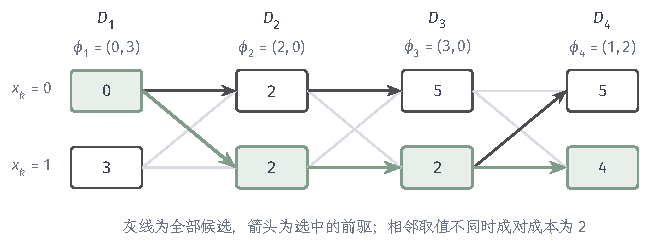
\includegraphics[width=109.587mm]{figures/01-basic-mathematics/04-graphs/tikz/c5-chain-recursion/figure.pdf}
  \caption{四变量二值链上的递推表。每列是一个变量，上下两格分别是$D_k(0)$与$D_k(1)$，列上方的小字为一元项。两列之间的灰色线表示全部候选，箭头从每个状态选中的前驱指向该状态，即回溯表$p_k$记录的选择。末列中$D_4(1)=4$最小，沿绿色箭头逆向读取得到最优配置$(0,1,1,1)$。逐点选取一元项最小的状态会得到$(0,1,1,0)$，成本为$5$。}
  \label{fig:graph-dp-chain-recursion}
\end{figure}

这个例子也说明了成对项的作用。若各变量只看自己的一元项，会选$(0,1,1,0)$：一元项合计为$1$，但两处取值变化要付$4$，总成本为$5$。递推得到的$(0,1,1,1)$在$x_4$上多付了$1$个单位的一元成本，却省掉了最后一处变化。

\paragraph{计算开销}
设每个变量至多有$q$个状态。每一轮要为$x_k$的每个状态比较至多$q$个候选，共至多$q^2$次候选计算，整条链约$nq^2$次。存储方面，每轮的$D_k$与回溯表$p_k$各至多$q$项，共约$2nq$项；若只要最优值而不恢复配置，任一时刻只需保留上一轮的表。与$q^n$次枚举相比，开销从指数降为线性于$n$。

\subsection{树上的递推}

\paragraph{从单个前驱到多个子树}
树没有链那样的天然顺序，但选定一个根$\rho$以后，每个非根顶点都有唯一的父点（第~\ref{sec:graph-trees-forests}节）。链上的$D_{k-1}$概括了$x_k$一侧的全部变量；在树上，一个顶点可能有多个子点，每个子点下面挂着一棵子树，需要分别概括后再合并。

对树的一条边$\{u,v\}$，删去它以后树分成两部分，记含$u$的那部分顶点集为$V_{u|v}$，称为$u$一侧。从$u$发往$v$的\term{消息}（message）是一张以$x_v$为索引的表，定义为
\begin{equation}
\begin{aligned}
m_{u\to v}(x_v)=\min_{x_u\in\mathcal X_u}\Bigl[&\phi_u(x_u)+\phi_{u,v}(x_u,x_v)\\
&+\sum_{r\in N(u)\setminus\{v\}}m_{r\to u}(x_u)\Bigr],
\end{aligned}
\label{eq:graph-dp-tree-message}
\end{equation}
其中$N(u)$是$u$在依赖图中的邻居集合。叶顶点只有一个邻居，求和为空，消息只由它自己的一元项和边上的成对项算出。下面的定理说明，这张表恰好概括了$u$一侧的全部成本。

\begin{theorem}[树上消息的含义]
\label{thm:graph-dp-tree-message}
设依赖图$\mathcal G=(V,E)$是有限树，总成本由式~\eqref{eq:graph-dp-pairwise-cost}给出。对任意边$\{u,v\}$，记$F_{u|v}$为$u$一侧的部分成本：$V_{u|v}$中各顶点的一元项、两端都在$V_{u|v}$中的成对项，再加上边$\{u,v\}$上的$\phi_{u,v}$。则对每个$x_v$，
\[
m_{u\to v}(x_v)=\min_{\bm x_{V_{u|v}}}F_{u|v}(\bm x_{V_{u|v}},x_v).
\]
进一步，对任意根$\rho$，$\min_{\bm x}F(\bm x)=\min_{x_\rho}\bigl[\phi_\rho(x_\rho)+\sum_{r\in N(\rho)}m_{r\to\rho}(x_\rho)\bigr]$。
\end{theorem}

\begin{proof}
对$|V_{u|v}|$归纳。删去$u$以后，$V_{u|v}\setminus\{u\}$按$u$的其他邻居$r\in N(u)\setminus\{v\}$分成互不相交的部分$V_{r|u}$。由树中路径的唯一性，不同部分之间没有边，否则会与$u$形成环。因此$F_{u|v}$可以拆成
\[
F_{u|v}=\phi_u(x_u)+\phi_{u,v}(x_u,x_v)+\sum_{r\in N(u)\setminus\{v\}}F_{r|u},
\]
其中每个$F_{r|u}$只依赖$x_u$与$\bm x_{V_{r|u}}$，并且每个局部项恰好出现在其中一处。固定$x_u$后，各$\bm x_{V_{r|u}}$是互不相交的变量组，由式~\eqref{eq:graph-dp-min-rules}后的第三条规则，对它们求最小值得到$\sum_r\min F_{r|u}$；由归纳假设，这个和等于$\sum_r m_{r\to u}(x_u)$。最后对$x_u$求最小值，就得到式~\eqref{eq:graph-dp-tree-message}。叶顶点是归纳的起点，此时求和为空，结论直接由定义得出。根处的等式用同样的拆分得到：$V\setminus\{\rho\}$按$\rho$的邻居分成互不相交的部分，每部分的最小成本是一条入消息。
\end{proof}

\paragraph{后序计算与分叉树算例}
式~\eqref{eq:graph-dp-tree-message}中，$u$发出消息前需要先收到来自其他邻居的消息。选定根后按后序处理顶点（先处理全部子点，再处理父点），每个顶点在收齐子点的消息后向父点发送一条消息，就满足了这个要求；最后在根处合并。图~\ref{fig:graph-dp-tree-messages}左半给出一个例子：树有边$\{1,3\},\allowbreak\{2,3\},\allowbreak\{3,4\},\allowbreak\{4,5\}$，以$3$为根；二值一元项为$\phi_1=(0,2)$、$\phi_2=(2,0)$、$\phi_3=(1,0)$、$\phi_4=(0,1)$、$\phi_5=(3,0)$；成对项在两端相同时为$0$，不同时分别为$1,1,2,1$（按上面边的顺序）。

后序为$1,2,5,4$。叶消息为$m_{1\to3}=(0,1)$，$m_{2\to3}=(1,0)$，$m_{5\to4}=(1,0)$，其中例如$m_{1\to3}(1)=\min(0+1,\,2+0)=1$。内部顶点$4$收到$m_{5\to4}$后向根发送
\[
\begin{aligned}
m_{4\to3}(x_3)&=\min_{x_4}\bigl[\phi_4(x_4)+\phi_{3,4}(x_3,x_4)+m_{5\to4}(x_4)\bigr]\\
&=\bigl(\min(0+0+1,\,1+2+0),\ \min(0+2+1,\,1+0+0)\bigr)=(1,1).
\end{aligned}
\]
根处合并一元项与三条入消息：$x_3=0$时为$1+0+1+1=3$，$x_3=1$时为$0+1+0+1=2$。因此最小总成本为$2$，根取$x_3=1$。整个计算只算了$4$条消息，每条消息比较$4$个候选，而枚举需要$2^5=32$个配置。

\begin{figure}[!htb]
  \centering
  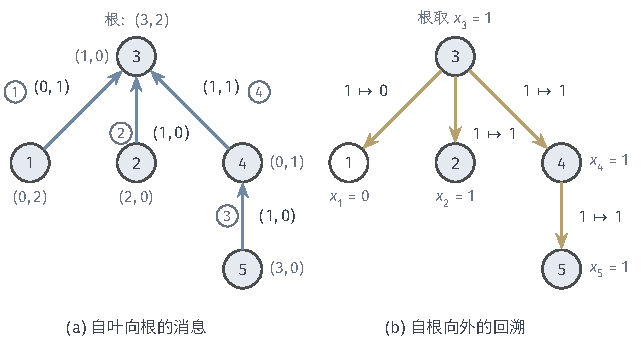
\includegraphics[width=108.514mm]{figures/01-basic-mathematics/04-graphs/tikz/c5-tree-messages/figure.pdf}
  \caption{分叉树上的消息与回溯。左：以$3$为根，按后序$1,2,5,4$发送消息；顶点旁的灰色二元组是一元项，箭头旁的二元组是消息表在接收端取$0$、$1$时的值，小圆圈中的序号是发送顺序；根合并后得到$(3,2)$。右：根取$x_3=1$后沿树向外查回溯表，黄色箭头旁的“$1\mapsto0$”表示父点取$1$时子点的最优选择为$0$；蓝色顶点取$1$，白色顶点取$0$，恢复的配置$(0,1,1,1,1)$成本为$2$。}
  \label{fig:graph-dp-tree-messages}
\end{figure}

\paragraph{每个顶点的最小成本表}
只求整体最优值时，一次自叶向根的计算已经足够。有时还需要知道每个顶点$v$取各个状态时整体能达到的最小成本，即$\min_{\bm x:\,x_v=s}F(\bm x)$。对根，这就是根处的合并结果；对其他顶点，还缺少来自父点一侧的消息。这时再按前序从根向叶发送一遍消息，同样使用式~\eqref{eq:graph-dp-tree-message}，然后在每个顶点合并全部入消息与一元项。仍以上例，从根发往$1$的消息为$m_{3\to1}=(2,1)$，于是$x_1$取$0$、$1$时的最小总成本为$(0+2,\,2+1)=(2,3)$，其最小值与整体最优值$2$一致。两遍计算共发送$2(n-1)$条消息；没有用到的方向不必计算。

\paragraph{计算开销}
每条消息对$x_v$的每个状态比较$x_u$的至多$q$个状态，每个候选要加上$|N(u)|$项，所以发出全部向上消息共需$O\bigl(\sum_u|N(u)|q^2\bigr)=O(nq^2)$次加法和比较，其中用到了树中$\sum_u|N(u)|=2(n-1)$。存储为$n-1$张消息表，每张至多$q$项。

\subsection{最优配置的回溯}

最优值只告诉我们最小成本是多少，并不直接给出达到它的配置。消息表经过了最小化，已经丢掉了“是哪一个$x_u$达到最小”的信息；若只保存最优值，事后只能重新枚举。解决办法是在计算每条消息时，为接收端的每个状态$x_v$同时记录达到最小值的$x_u$，组成一张\term{回溯表}$b_{u\to v}(x_v)$。并列最优时需要事先固定选择规则，本节约定取编号最小的状态。

\paragraph{从根向外读取}
回溯从根开始：取使根处合并值最小的$x_\rho$；然后按前序，对每个已确定取值的顶点$v$及其子点$u$，令$x_u=b_{u\to v}(x_v)$。由于每个子点只由父点的取值决定，这一过程沿树向外恰好给每个变量赋值一次。在图~\ref{fig:graph-dp-tree-messages}右半中，根取$x_3=1$；查表得$b_{1\to3}(1)=0$、$b_{2\to3}(1)=1$、$b_{4\to3}(1)=1$；再由$x_4=1$得$b_{5\to4}(1)=1$。恢复的配置为$(x_1,\ldots,x_5)=(0,1,1,1,1)$。

回溯得到的配置确实达到最优值。对子树大小归纳可知：若$x_v$已经确定，按回溯表给$u$一侧赋值后，$u$一侧的部分成本$F_{u|v}$恰好等于$m_{u\to v}(x_v)$，因为每一步选的$x_u$都达到式~\eqref{eq:graph-dp-tree-message}中的最小值，而子树内部又由归纳假设达到各条入消息的值。在根处合并后，总成本就等于根处的最小合并值。图~\ref{fig:graph-dp-chain-recursion}中的绿色箭头是链上的同一过程。

\paragraph{结果核对与不可行情形}
把恢复的配置代回全部原始局部项，可以独立核对结果。上例中一元项依次为$0,0,0,1,0$，合计$1$；成对项中只有边$\{1,3\}$两端不同，贡献$1$；总成本为$2$，与根处的值一致，而且每个局部项只计了一次。这样的核对不依赖消息计算本身，能发现表格或下标上的错误。

若根处的最小合并值为$+\infty$，说明每个配置都被某个局部项禁止，问题没有可行配置。这时应直接报告不可行，而不是把回溯得到的配置当作最优解输出，因为在全为$+\infty$的表中任何选择都“达到”最小值。另外，回溯表只恢复一个最优配置；若要列出全部并列最优的配置，需要在每个状态记录全部最优选择，而这类配置的数目本身可能随$n$指数增长。

% 第5章第3节：变量消元（消元操作与不变量、中间函数与填充边、消元次序与计算开销）。

\section{变量消元}
\label{sec:graph-variable-elimination}

链和树上的递推每次处理一个端点：把只连着已处理部分的变量汇总掉，留下一张接口表。一般依赖图可能有环，局部函数也可能读取三个以上变量，这时不一定存在只连着一个邻居的变量。本节把“汇总一个变量”写成对局部函数集合的一般操作，说明按任意次序逐个汇总都给出正确的最优值；随后会看到，正确性不依赖次序，中间表的大小却依赖次序。

本节沿用第~\ref{sec:graph-local-functions}节的四变量例子：二值变量$x_1,\ldots,x_4$，两个三元局部函数$\phi_A(x_1,x_2,x_3)$与$\phi_B(x_2,x_3,x_4)$，总成本$F=\phi_A+\phi_B$。两张表由表~\ref{tab:graph-dp-ternary-tables}给出，其中$+\infty$表示禁止的组合。

\begin{table}[!htb]
  \centering
  \caption{四变量例子的两个三元局部函数。第一列的三位二进制串对$\phi_A$表示$(x_1,x_2,x_3)$，对$\phi_B$表示$(x_2,x_3,x_4)$。}
  \label{tab:graph-dp-ternary-tables}
  \begin{tabular}{ccccccccc}
    \toprule
    取值 & $000$ & $001$ & $010$ & $011$ & $100$ & $101$ & $110$ & $111$\\
    \midrule
    $\phi_A(x_1,x_2,x_3)$ & $1$ & $0$ & $2$ & $+\infty$ & $0$ & $2$ & $1$ & $2$\\
    $\phi_B(x_2,x_3,x_4)$ & $2$ & $1$ & $0$ & $+\infty$ & $+\infty$ & $0$ & $1$ & $2$\\
    \bottomrule
  \end{tabular}
\end{table}

\subsection{消元操作}

\paragraph{汇总一个变量}
设当前有一组局部函数$\mathcal F$，总成本是它们的和。要汇总变量$x_i$，先找出所有作用域含$i$的函数，记为$\mathcal F_i$；它们的作用域之并去掉$i$，记为$R_i$。固定$R_i$中变量的取值后，把$\mathcal F_i$中的函数相加，再对$x_i$取最小，得到一个新函数
\begin{equation}
\psi_i(\bm x_{R_i})=\min_{x_i\in\mathcal X_i}\sum_{f\in\mathcal F_i}f .
\label{eq:graph-dp-elimination-step}
\end{equation}
然后从$\mathcal F$中删去$\mathcal F_i$，加入$\psi_i$；不含$i$的函数保持原样。这一操作称为消去$x_i$，逐个消去变量的方法称为\term{变量消元}（variable elimination）。链上的$m_{1\to2}$正是消去$x_1$时得到的新函数。

在四变量例子中消去$x_1$：只有$\phi_A$含$1$，$R_1=\{2,3\}$。对$(x_2,x_3)=(0,0),(0,1),(1,0),(1,1)$，分别比较$x_1=0,1$两行，得到
\[
\psi_1(x_2,x_3)=\bigl(\min(1,0),\ \min(0,2),\ \min(2,1),\ \min(+\infty,2)\bigr)=(0,\,0,\,1,\,2),
\]
达到最小值的$x_1$依次为$1,0,1,1$。消元后的函数集合是$\{\psi_1,\phi_B\}$。可以逐项核对它没有改变剩余变量的最优成本：例如取$(x_2,x_3,x_4)=(1,0,1)$，原问题对$x_1$求最小值为$\min\bigl(\phi_A(0,1,0)+\phi_B(1,0,1),\ \phi_A(1,1,0)+\phi_B(1,0,1)\bigr)=\min(2,1)=1$，新集合给出$\psi_1(1,0)+\phi_B(1,0,1)=1+0=1$，两者相同。

\paragraph{不变量与正确性}
上面的核对对每个剩余配置都成立，这不是巧合。设已经按某个次序消去了下标集合$Z$中的变量，把剩余变量的一个配置记为$\bm y=\bm x_{V\setminus Z}$。消元过程保持下面的不变量：
\begin{equation}
\sum_{f\in\mathcal F}f(\bm y)=\min_{\bm x_Z}F(\bm x_Z,\bm y)\qquad\text{对每个剩余配置}\ \bm y .
\label{eq:graph-dp-elimination-invariant}
\end{equation}

\begin{theorem}[变量消元的正确性]
\label{thm:graph-dp-elimination}
设各变量的状态集合有限，总成本由式~\eqref{eq:graph-dp-local-sum}给出。从$\mathcal F=\{\phi_a:a\in A\}$出发，按任意次序反复执行式~\eqref{eq:graph-dp-elimination-step}的消元操作，则每一步之后不变量~\eqref{eq:graph-dp-elimination-invariant}都成立。特别地，消去全部变量后剩下的常数（无变量的函数之和）等于$\min_{\bm x}F(\bm x)$；只消去$V\setminus Q$中的变量时，剩余函数之和是关于$\bm x_Q$的表，在每个$\bm x_Q$处等于$\min_{\bm x_{V\setminus Q}}F(\bm x)$。
\end{theorem}

\begin{proof}
开始时$Z=\varnothing$，当前函数之和就是$F$，不变量成立。设消去$x_i$之前不变量对$Z$成立。把当前函数分为含$i$的$\mathcal F_i$与其余部分$\mathcal F_{-i}$。固定$Z\cup\{i\}$以外的变量后，$\mathcal F_{-i}$中各函数的值与$x_i$无关，按式~\eqref{eq:graph-dp-min-rules}可以移出对$x_i$的最小化：
\[
\min_{x_i}\Bigl[\sum_{f\in\mathcal F_{-i}}f+\sum_{f\in\mathcal F_i}f\Bigr]
=\sum_{f\in\mathcal F_{-i}}f+\min_{x_i}\sum_{f\in\mathcal F_i}f
=\sum_{f\in\mathcal F_{-i}}f+\psi_i .
\]
右端正是消元后的函数之和。左端由不变量等于$\min_{x_i}\min_{\bm x_Z}F$，再由式~\eqref{eq:graph-dp-min-rules}的第一条等于$\min_{\bm x_{Z\cup\{i\}}}F$。所以不变量对$Z\cup\{i\}$成立。对消元步数归纳即得结论。
\end{proof}

\begin{algorithm}[变量消元求最小成本]
\label{alg:graph-dp-variable-elimination}
输入：有限状态集合、局部函数表、一个消元次序。输出：最小成本，以及（若需要）一个最优配置。
\begin{enumerate}
  \item 按次序取下一个变量$x_i$，找出当前全部含$i$的函数$\mathcal F_i$，确定$R_i$。
  \item 对$\bm x_{R_i}$的每个取值，枚举$x_i$的全部状态，按式~\eqref{eq:graph-dp-elimination-step}求$\psi_i$；同时把达到最小值的$x_i$（并列取编号最小者）记入回溯表$b_i(\bm x_{R_i})$。
  \item 用$\psi_i$替换$\mathcal F_i$，重复直到变量全部消去，剩下的常数即最小成本。
  \item 若最小成本有限，按消元的逆序依次令$x_i=b_i(\bm x_{R_i})$；由于$R_i$中的变量都比$x_i$晚消去，查表时它们已经取定。
\end{enumerate}
\end{algorithm}

逆序回溯的正确性与树上相同：每一步选的$x_i$达到式~\eqref{eq:graph-dp-elimination-step}的最小值，于是按逆序逐步代回不变量，恢复的配置使$F$等于最小成本。若只保存$\psi_i$而不保存回溯表，就无法恢复配置。

\subsection{中间函数与填充边}

消去一个变量时，新函数$\psi_i$的作用域$R_i$由所有含$i$的函数共同决定。在原始图上看，$R_i$恰好是$i$在当前原始图中的邻居集合：两个变量相邻，当且仅当它们同在某个当前函数的作用域中。新函数读取这些邻居的联合取值，所以消元后的原始图中，这些邻居两两相邻。

\paragraph{消去一个连着三个邻居的变量}
在四变量例子中改为先消去$x_2$。$\phi_A$与$\phi_B$都含$2$，$R_2=\{1,3\}\cup\{3,4\}=\{1,3,4\}$，新函数
\[
\psi_2(x_1,x_3,x_4)=\min_{x_2}\bigl[\phi_A(x_1,x_2,x_3)+\phi_B(x_2,x_3,x_4)\bigr]
\]
同时读取$x_1,x_3,x_4$。原始图中原来没有边$\{1,4\}$，消元后必须补上，如图~\ref{fig:graph-dp-elimination-step}所示。这样为记录新函数的联合依赖而补入的边称为\term{填充边}（fill-in edge）。填充边不表示原问题增加了约束：原来$x_1$与$x_4$通过$x_2$间接联系，消去$x_2$以后，这种间接联系只能由新函数直接记录。

\begin{figure}[!htb]
  \centering
  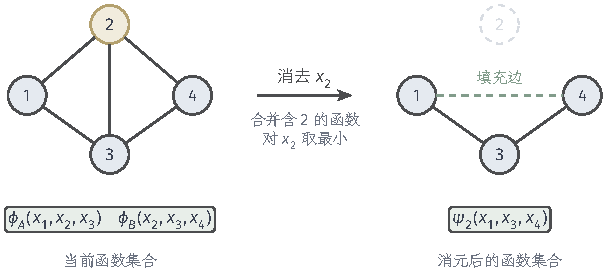
\includegraphics[width=102.687mm]{figures/01-basic-mathematics/04-graphs/tikz/c5-elimination-step/figure.pdf}
  \caption{消去$x_2$时的函数更新与图更新。左：消元前，黄色的$x_2$同时属于$\phi_A$与$\phi_B$的作用域，它的邻居是$1,3,4$。右：消元后，两个函数被新函数$\psi_2(x_1,x_3,x_4)$取代，$x_2$及其关联边被删除，邻居$1,3,4$两两相邻，其中绿色虚线$\{1,4\}$是填充边。}
  \label{fig:graph-dp-elimination-step}
\end{figure}

一般地，消元在原始图上对应一个纯粹的结构操作：把$i$的当前邻居两两连边，然后删去$i$及其关联边。不含$i$的函数提供的边保持不变；含$i$的函数在剩余变量之间提供的边都落在$R_i$内，已被补成的团覆盖。因此，消元后函数集合的原始图恰好是对原始图执行这一操作的结果。

\paragraph{数值计算与结构记账}
图上的操作只预测新函数可能同时读取哪些变量，不计算新函数的取值。对特殊的局部函数，新函数可能仍能进一步分解。例如，若$\phi_A(x_1,x_2,x_3)=g(x_1)+h(x_2,x_3)$，则
\[
\psi_2(x_1,x_3,x_4)=g(x_1)+\min_{x_2}\bigl[h(x_2,x_3)+\phi_B(x_2,x_3,x_4)\bigr],
\]
它是一个$x_1$的函数与一个$(x_3,x_4)$的函数之和，实际上并不需要同时索引$x_1$与$x_4$。图上的填充边不知道这种数值巧合，所以补边图给出的是通用情形下的作用域上界。后面讨论树分解时只使用这种结构记账：它适用于作用域给定、函数值任意的全部问题；具体函数是否还能化简，要回到数值表本身判断。

\subsection{消元次序与计算开销}

定理~\ref{thm:graph-dp-elimination}允许任意消元次序，不同次序给出相同的最优值，但中间函数的大小可以相差很多。下面在四变量例子上比较两个\term{消元次序}（elimination order）：$(1,4,2,3)$与$(2,1,3,4)$。

\paragraph{两种次序的逐步对照}
按$(1,4,2,3)$：消去$x_1$得到上面的$\psi_1(x_2,x_3)=(0,0,1,2)$；消去$x_4$时只有$\phi_B$含$4$，得到$\psi_4(x_2,x_3)=\min_{x_4}\phi_B=(1,0,0,1)$；消去$x_2$时合并$\psi_1,\psi_4$，得到只依赖$x_3$的表（记为$\psi_2'$，以区别于上面先消$x_2$时的$\psi_2$）$\psi_2'(x_3)=\bigl(\min(0+1,1+0),\ \min(0+0,2+1)\bigr)=(1,0)$；最后消去$x_3$得常数$0$。

按$(2,1,3,4)$消元时，第一步就要在$x_1,x_3,x_4$的$8$种取值下各比较$x_2$的两种状态，得到$8$项的$\psi_2$；其后得到的表依次为$(x_3,x_4)$上的$(2,1,0,4)$、$x_4$上的$(0,1)$，最后同样得常数$0$。表~\ref{tab:graph-dp-elimination-orders}列出了每一步的作用域和规模，图~\ref{fig:graph-dp-elimination-orders}画出了对应的图变化。

\begin{table}[!htb]
  \centering
  \caption{四变量例子上两种消元次序的逐步规模。“枚举”指计算新函数时要比较的候选组合数，即$R_i\cup\{i\}$上的配置数；“输出”指新函数表的项数，回溯表的项数与之相同。}
  \label{tab:graph-dp-elimination-orders}
  \begin{tabular}{cccccccc}
    \toprule
    \multicolumn{4}{c}{次序$(1,4,2,3)$} & \multicolumn{4}{c}{次序$(2,1,3,4)$}\\
    \cmidrule(lr){1-4}\cmidrule(lr){5-8}
    消去 & 新作用域 & 枚举 & 输出 & 消去 & 新作用域 & 枚举 & 输出\\
    \midrule
    $x_1$ & $\{2,3\}$ & $8$ & $4$ & $x_2$ & $\{1,3,4\}$ & $16$ & $8$\\
    $x_4$ & $\{2,3\}$ & $8$ & $4$ & $x_1$ & $\{3,4\}$ & $8$ & $4$\\
    $x_2$ & $\{3\}$ & $4$ & $2$ & $x_3$ & $\{4\}$ & $4$ & $2$\\
    $x_3$ & $\varnothing$ & $2$ & $1$ & $x_4$ & $\varnothing$ & $2$ & $1$\\
    \midrule
    合计 & & $22$ & $11$ & 合计 & & $30$ & $15$\\
    \bottomrule
  \end{tabular}
\end{table}

\begin{figure}[!htb]
  \centering
  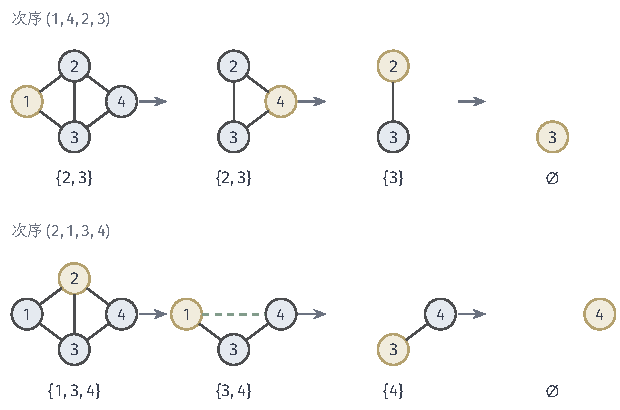
\includegraphics[width=105.004mm]{figures/01-basic-mathematics/04-graphs/tikz/c5-elimination-orders/figure.pdf}
  \caption{两种消元次序下原始图的变化。上行按$(1,4,2,3)$消元，每一步被消去的黄色顶点的邻居都已两两相邻，不产生填充边，新函数至多读取两个变量。下行按$(2,1,3,4)$消元，消去$2$时要补入填充边$\{1,4\}$（第二个图中的绿色虚线），新函数读取三个变量。每个图下方标出消去黄色顶点后新函数的作用域。}
  \label{fig:graph-dp-elimination-orders}
\end{figure}

两种次序都正确，也都恢复出同一个最优配置：$x_1=0$，$x_2=0$，$x_3=1$，$x_4=0$，代回表~\ref{tab:graph-dp-ternary-tables}得$\phi_A(0,0,1)+\phi_B(0,1,0)=0+0=0$。差别在于规模：第一种次序的最大中间表只有$4$项，第二种有$8$项。在这个小例子里差别不大；但若每个变量有$q$个状态，读取$r$个变量的表就有$q^r$项，多读取一个变量意味着表扩大$q$倍。

\paragraph{每一步的开销}
设消去$x_i$时$|R_i|=r_i$，各变量至多$q$个状态。计算$\psi_i$要对$R_i\cup\{i\}$的至多$q^{r_i+1}$种取值，各读取$\mathcal F_i$中每个函数一次，时间约为$|\mathcal F_i|\,q^{r_i+1}$；输出表与回溯表各至多$q^{r_i}$项。整个消元的时间由各步之和给出，主导项来自$r_i$最大的那一步。查找含$i$的函数还需要按变量维护的函数索引，这部分开销与函数个数成正比。

所以变量消元的规模取决于“最多同时处理多少个变量”，即$\max_i(r_i+1)$。这个数由依赖图和消元次序共同决定：有限状态并不保证精确消元总是可行，在某些图上，无论怎样排序，都会有一步需要同时处理很多变量。下一节用树分解描述这些同时处理的变量组，并用树宽给出与次序无关的结构度量。

% 第5章第4节：树分解与树宽（袋与接口、树分解的三个条件、团必被某袋容纳、宽度与树宽）。

\section{树分解与树宽}
\label{sec:graph-tree-decomposition}

上一节看到，变量消元的开销取决于每一步同时处理的变量组。本节把这些变量组单独拿出来，研究它们怎样组织成一棵树，才能让计算沿树进行而不丢失一致性。先从消元过程引出“袋”和“接口”，再给出合法分解的三个条件，最后用袋的大小定义宽度和树宽。本节只讨论结构本身：怎样构造分解放在第~\ref{sec:graph-tree-decomposition-construction}节，怎样在分解上计算放在第~\ref{sec:graph-bag-dp}节。

\subsection{袋与接口}

\paragraph{从消元步骤到袋}
回到四变量例子的次序$(1,4,2,3)$。消去$x_1$时要同时处理$\{1\}\cup R_1=\{1,2,3\}$，消去$x_4$时处理$\{2,3,4\}$，随后依次处理$\{2,3\}$和$\{3\}$。每一步产生的新函数会在后面某一步被用到：$\psi_1$与$\psi_4$都在消去$x_2$时被合并，$\psi_2'$在消去$x_3$时被使用。把每一步同时处理的变量集合看成一个节点，按“新函数交给哪一步使用”连接这些节点，就得到图~\ref{fig:graph-dp-bags-interface}中间的一棵树。

这种准备放进同一张表里同时索引的变量集合称为\term{袋}（bag），袋组成的树称为袋树。袋树的节点是计算单元，袋树的边表示两个计算单元之间传递一张表；它与原始图中连接两个变量的边含义不同。不同的袋可以有公共变量，例如$\{1,2,3\}$与$\{2,3,4\}$都含$2,3$。

\begin{figure}[!htb]
  \centering
  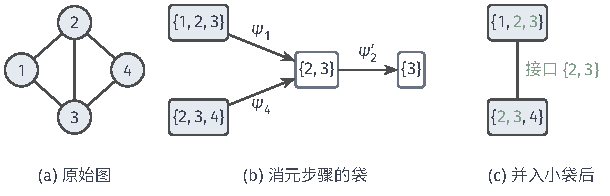
\includegraphics[width=103.283mm]{figures/01-basic-mathematics/04-graphs/tikz/c5-elimination-to-bags/figure.pdf}
  \caption{从消元步骤得到袋。左：四变量例子的原始图。中：按次序$(1,4,2,3)$消元时，每一步同时处理的变量集合构成一个袋，箭头表示新函数交给哪一步使用。右：$\{2,3\}$和$\{3\}$已包含在相邻的大袋中，并入后只剩两个袋，它们的交集$\{2,3\}$（绿色）就是接口。}
  \label{fig:graph-dp-bags-interface}
\end{figure}

袋与原始图中的“团”有关，但不必是团。原始图中两两相邻的顶点集合称为\term{团}（clique）。四变量例子中$\{1,2,3\}$是团，$\{1,2,4\}$不是，因为缺边$\{1,4\}$。按次序$(2,1,3,4)$消元时，第一步要同时处理$\{1,2,3,4\}$，这个袋在原始图中不是团，只在补入填充边后才成为团。所以袋可以重叠，也可以含有原图中不相邻的变量。

\paragraph{接口}
袋$\{2,3\}$和$\{3\}$都已包含在相邻的大袋中，可以并入，最后只剩两个袋$\{1,2,3\}$与$\{2,3,4\}$，如图~\ref{fig:graph-dp-bags-interface}右侧。相邻两袋的交集称为它们的接口（interface），这里是$\{2,3\}$。接口上的变量在两个袋里是同一个变量，不是两个副本：左袋在汇总$x_1$时必须对$(x_2,x_3)$的每种取值分别给出结果，右袋使用这些结果时也必须按同样的$(x_2,x_3)$取值来读。左袋的结果正是$\psi_1(x_2,x_3)$，一张以接口为索引的表。

由此提出一个要求。若某个变量出现在两个不相邻的袋中，而连接它们的袋树路径上有某个袋不含这个变量，那么两侧的计算无法通过接口约定这个变量取同一个值。为了让每个变量的取值在它出现的所有袋之间保持一致，袋的连接方式必须受到限制。下面把这个要求与覆盖要求一起写成定义。

\subsection{树分解的条件}

\paragraph{三个条件}
袋必须能容纳所有局部函数，袋之间的连接又必须保证一致。结构上，前一项要求每个变量和原始图的每条边都被某个袋包含，后一项就是上面提出的连接要求。

\begin{definition}[树分解]
\label{def:graph-dp-tree-decomposition}
设$\mathcal G=(V,E)$是有限无向图。$\mathcal G$的一个\term{树分解}（tree decomposition）由一棵有限树$\mathcal T$（节点集记为$T$）和每个节点$t\in T$上的子集$B_t\subseteq V$组成，满足：
\begin{enumerate}
  \item 顶点覆盖：每个顶点$v\in V$至少属于一个袋；
  \item 边覆盖：对每条边$\{u,v\}\in E$，存在某个袋同时含有$u$与$v$；
  \item 运行交集：对每个顶点$v\in V$，含$v$的节点集合$T_v=\{t\in T:v\in B_t\}$在$\mathcal T$中连通。
\end{enumerate}
第三个条件称为\term{运行交集性质}（running intersection property）。
\end{definition}

运行交集等价于：若$v$同时属于$B_s$和$B_t$，则$\mathcal T$中从$s$到$t$的路径上每个袋都含$v$。因为树中两点之间只有一条路径，$T_v$连通恰好意味着这条路径留在$T_v$中。

\paragraph{只覆盖边还不够}
图~\ref{fig:graph-dp-running-intersection}比较路径$1-2-3-4$上的两种袋连接。两种连接使用同样的三个袋$\{1,2\},\allowbreak\{2,3\},\allowbreak\{3,4\}$，都覆盖了全部顶点和边。上面一种按$\{1,2\}-\{2,3\}-\{3,4\}$连接，含$2$的两个袋相邻，含$3$的两个袋也相邻，是树分解。下面一种按$\{1,2\}-\{3,4\}-\{2,3\}$连接，含$2$的两个袋被不含$2$的袋$\{3,4\}$隔开。若沿这棵树计算，左端的袋可以选$x_2=0$，右端的袋可以选$x_2=1$，中间的袋不记录$x_2$，无从发现矛盾；拼起来的结果不对应任何一个配置。

\begin{figure}[!htb]
  \centering
  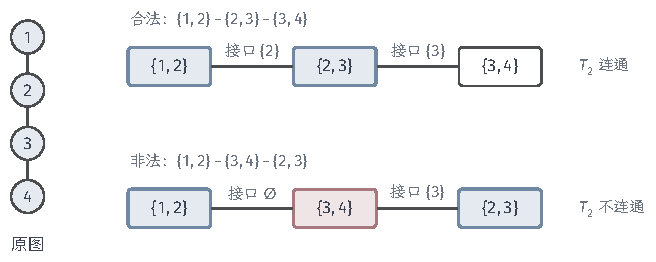
\includegraphics[width=111.016mm]{figures/01-basic-mathematics/04-graphs/tikz/c5-running-intersection/figure.pdf}
  \caption{路径$1-2-3-4$上的合法与非法袋连接。两种连接使用相同的三个袋，都覆盖全部顶点和边。上：含$2$的袋（蓝色）彼此相邻，含$3$的袋也相邻，满足运行交集。下：含$2$的两个袋之间隔着不含$2$的袋$\{3,4\}$（红色），$T_2$不连通，不是树分解。}
  \label{fig:graph-dp-running-intersection}
\end{figure}

\paragraph{完整作用域总能放进某个袋}
计算时每个局部函数要整个放进一个袋，因为袋表需要同时索引它的全部变量。一个作用域$S_a$在原始图上是团：其中任意两个变量同在$\phi_a$中，因而相邻。但树分解的定义只要求每条边被某个袋覆盖，三个变量两两成边时，三条边可能分别落在三个不同的袋中。下面的引理说明这种情况不会发生。

把每个顶点$v$的出现位置$T_v$看成袋树中的一棵连通子树。若$u,v$相邻，边覆盖给出一个同时含$u,v$的袋，于是$T_u$与$T_v$相交。对一个团$C$，各$T_v$（$v\in C$）两两相交；要证明的是它们有一个公共节点。

\begin{lemma}[团被某个袋容纳]
\label{lem:graph-dp-clique-in-bag}
设$(\mathcal T,\{B_t\}_{t\in T})$是$\mathcal G$的树分解，$C\subseteq V$是$\mathcal G$中的非空团，则存在节点$t\in T$使$C\subseteq B_t$。
\end{lemma}

\begin{proof}
任取袋树的一个节点作为根。对每个$v\in C$，$T_v$非空且连通。先说明$T_v$中有唯一一个离根最近的节点，记为$r_v$，并且$T_v$的每个节点都是$r_v$的后代（含$r_v$本身）。若$y\in T_v$不是$r_v$的后代，从$y$到$r_v$的树上路径要先向上经过$y$与$r_v$的最近公共祖先$z$，而$z$比$r_v$更靠近根；由$T_v$连通，这条路径留在$T_v$中，于是$z\in T_v$，与$r_v$的选取矛盾。同样的论证也说明离根最近的节点唯一。

在$C$中取一个顶点$w$，使$r_w$的深度在$\{r_v:v\in C\}$中最大。下面证明$r_w$属于每个$T_u$（$u\in C$）。$u=w$时，$r_w\in T_w$由定义成立。$u\neq w$时，$u,w$相邻，所以$T_u\cap T_w$中有某个节点$x$；$x\in T_w$，因而$x$是$r_w$的后代。考察$T_u$中从$x$到$r_u$的路径，它留在$T_u$中。若$r_u$不是$r_w$的后代，这条路径从$r_w$子树内部走到外部，必须经过$r_w$，于是$r_w\in T_u$。若$r_u$是$r_w$的后代，则$r_u$的深度不小于$r_w$的深度；而按$w$的选取，$r_u$的深度又不大于$r_w$的深度，所以$r_u=r_w$，同样有$r_w\in T_u$。因此$r_w$属于全部$T_u$，袋$B_{r_w}$含有整个$C$。
\end{proof}

图~\ref{fig:graph-dp-clique-in-bag}画出了证明中的几棵子树：每个变量的出现位置向上延伸到自己的最高节点，最高节点最深的那个变量，它的最高节点被其余各子树“经过”，因而就是要找的袋。

\begin{figure}[!htb]
  \centering
  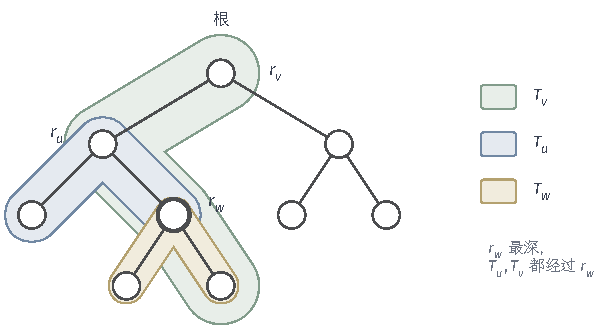
\includegraphics[width=102.648mm]{figures/01-basic-mathematics/04-graphs/tikz/c5-clique-in-bag/figure.pdf}
  \caption{团$\{u,v,w\}$被某个袋容纳的论证。袋树以顶部节点为根，三种颜色的区域分别是$T_u$、$T_v$、$T_w$，标签$r_u,r_v,r_w$标出各自离根最近的节点。$r_w$最深；$T_u$、$T_v$都要与$T_w$相交，而它们的最高节点不比$r_w$深，所以必须经过$r_w$。粗圈节点$r_w$的袋同时含$u,v,w$。}
  \label{fig:graph-dp-clique-in-bag}
\end{figure}

由引理~\ref{lem:graph-dp-clique-in-bag}，原始图的任一树分解中，每个局部函数的完整作用域都被某个袋整体容纳。因此在原始图上构造树分解就足够了，不需要额外记录高阶作用域；第~\ref{sec:graph-local-functions}节所说的“结构以原始图为依据、计算保留完整函数”在这里得到保证。

\subsection{宽度与树宽}

袋越大，袋表越大。为了用一个数概括一次分解的规模，定义树分解的宽度为$\max_{t\in T}|B_t|-1$，即最大袋的大小减一；图$\mathcal G$的\term{树宽}（treewidth）是它的全部树分解宽度的最小值，记为$\operatorname{tw}(\mathcal G)$。减一是一种约定，使得下面的树恰好宽度为一。

\paragraph{三个小例子}
单个顶点的图只需一个袋$\{1\}$，宽度为$0$，任何没有边的图都如此。至少含一条边的树宽度为$1$：任选根$\rho$，为每个非根顶点$u$建袋$\{u,p(u)\}$，其中$p(u)$是父点；若$p(u)$不是根，就把这个袋连到$p(u)$自己的袋上，根的各子点的袋则依次连成一条链。这样，非根顶点$v$出现在自己的袋和各子点的袋中，后者都与前者相邻；根只出现在各子点的袋中，它们连成链，所以运行交集成立。另一方面，一条边要求某个袋含两个顶点，宽度不能小于$1$。

四个顶点的环$1-2-3-4-1$有宽度为$2$的树分解：两个袋$\{1,2,3\}$与$\{1,3,4\}$，以一条边相连，接口为$\{1,3\}$。它没有宽度为$1$的树分解。证明沿用引理~\ref{lem:graph-dp-clique-in-bag}的思路：给任一树分解选根，在环上取$w$使$r_w$最深，$w$在环上的两个邻居$u,v$各自与$w$相邻，于是$T_u$、$T_v$都与$T_w$相交，上面的论证表明$r_w\in T_u\cap T_v$。这个袋含$u,v,w$三个顶点，所以宽度至少为$2$。这一论证对任何环都适用：含环的图树宽至少为$2$，树宽为$1$的图恰好是至少含一条边的森林（森林的各个分量分别按上面的方法分解，再用任意的边把各分量的袋树连成一棵树；不同分量没有公共顶点，这些连接不影响运行交集）。

这几个例子说明，树宽衡量的是图与树的接近程度：一条边需要两个变量同时出现，一个环则迫使某处至少三个变量同时出现。还要注意，某一次构造得到宽度$k$，只说明$\operatorname{tw}(\mathcal G)\leq k$；要断言树宽恰为$k$，还需要像上面那样证明不存在更小宽度的分解。

\paragraph{宽度与表的大小}
若每个变量至多有$q$个状态，宽度为$k$的分解中，每个袋至多有$k+1$个变量，稠密存储的袋表至多$q^{k+1}$项。这是第~\ref{sec:graph-bag-dp}节中主要的枚举规模。实际的总开销还包括袋的个数、接口的大小和每次读取局部函数的成本，宽度只控制其中随状态数指数增长的那一部分。

最后，寻找树宽最小的分解与使用一个已经给定的分解是两项不同的任务。前者在一般图上是困难的组合问题；后者只需检查三个条件并沿树计算。第~\ref{sec:graph-tree-decomposition-construction}节给出的构造方法都只保证得到合法的分解和宽度上界。

% 第5章第5节：树分解的构造（由消元次序构造、最小度与最小填充、弦图与完美消元序、团树与最大权生成树）。

\section{树分解的构造}
\label{sec:graph-tree-decomposition-construction}

上一节给出了树分解的合法性条件，但没有说明怎样得到一个分解。本节先说明，任何一个完整的消元次序都能机械地产生一个树分解，其宽度就是该次序下最大的中间作用域；再讨论没有给定次序时怎样选择次序。最后考虑一类不需要补边的图，即弦图，在其上可以直接用极大团作袋，并用第~\ref{sec:graph-minimum-spanning-tree}节的最大权生成树把它们连成团树。与第~\ref{sec:graph-variable-elimination}节不同，本节只做结构上的操作：输出袋和袋之间的连接，不计算任何成本表。

\subsection{基于消元次序的构造}

\paragraph{逐轮记录袋}
输入非空有限无向图$\mathcal G=(V,E)$和一个包含每个顶点恰好一次的消元次序$\pi$。按$\pi$逐个处理顶点：处理$v$时，读出$v$在当前图中的邻居集合，记为$N^+_\pi(v)$（上标$+$表示这些邻居都在次序中排在$v$之后）；记录袋$B_v=\{v\}\cup N^+_\pi(v)$；把$N^+_\pi(v)$中的顶点两两连边，然后删去$v$及其关联边。这正是第~\ref{sec:graph-variable-elimination}节中消元在原始图上的结构操作，袋$B_v$就是消去$x_v$时同时处理的变量组。

关键在于每一轮都要从更新后的图读取邻居。图~\ref{fig:graph-dp-elimination-to-decomposition}的例子有边$\{1,2\},\allowbreak\{1,4\},\allowbreak\{2,3\},\allowbreak\{3,4\},\allowbreak\{3,5\},\allowbreak\{4,5\}$，次序为$(1,2,5,3,4)$。处理$1$时，邻居$2,4$不相邻，补入填充边$\{2,4\}$，记袋$\{1,2,4\}$。处理$2$时，当前邻居是$\{3,4\}$，其中$4$是刚补入的邻居，记袋$\{2,3,4\}$。若误从原图读取，$2$的剩余邻居只有$3$，袋$\{2,3\}$就漏掉了消去$x_1$后新函数同时读取的$x_2,x_4$。随后依次记袋$\{3,4,5\}$、$\{3,4\}$、$\{4\}$，不再需要补边。

\paragraph{连接父袋}
袋记录完毕后，对每个$N^+_\pi(v)$非空的顶点$v$，令$p(v)$为$N^+_\pi(v)$中在次序里最早的顶点，把$B_v$连到$B_{p(v)}$；$N^+_\pi(v)$为空的袋没有父袋，作为根。原图不连通时会有多个根，可以再用任意边把这些根连成一棵树，这些边的接口为空。在上例中$p(1)=2$、$p(2)=3$、$p(5)=3$、$p(3)=4$，得到以$B_4=\{4\}$为根的袋树，最大袋含$3$个顶点，宽度为$2$。

\begin{figure}[!htb]
  \centering
  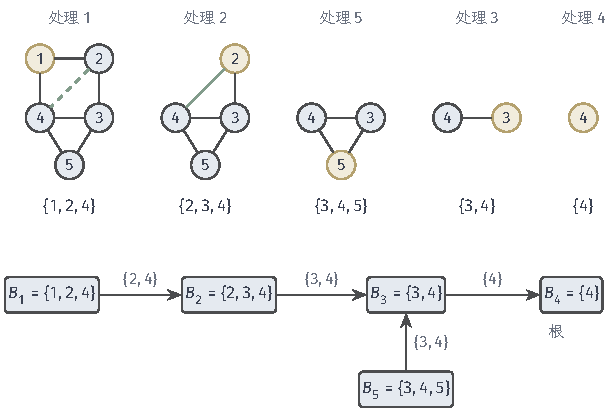
\includegraphics[width=104.369mm]{figures/01-basic-mathematics/04-graphs/tikz/c5-elimination-to-decomposition/figure.pdf}
  \caption{由消元次序$(1,2,5,3,4)$构造树分解。上行：每一轮的当前图，黄色为正在处理的顶点，绿色虚线为本轮补入的填充边，下一轮中它以绿色实线留在当前图里；图下标出记录的袋。下：按“连到最早被处理的后续邻居”连接父袋得到的袋树，箭头指向父袋，边旁标出接口。}
  \label{fig:graph-dp-elimination-to-decomposition}
\end{figure}

下面的定理说明这样得到的结构总是树分解。消元次序$\pi$下的最大后续邻居数$\max_v|N^+_\pi(v)|$称为$\pi$的\term{诱导宽度}（induced width）。

\begin{theorem}[消元次序产生树分解]
\label{thm:graph-dp-elimination-decomposition}
设$\mathcal G$是非空有限无向图，$\pi$是它的完整消元次序。按上面的方法记录袋$B_v=\{v\}\cup N^+_\pi(v)$并连接父袋（多个根之间用空接口边连接），得到的是$\mathcal G$的树分解，其宽度等于$\pi$的诱导宽度。因此$\mathcal G$的树宽不超过任何消元次序的诱导宽度。
\end{theorem}

\begin{proof}
先说明袋树是树。每个非根袋恰有一条通向父袋的边，而父点$p(v)$在次序中排在$v$之后，沿父边前进时次序位置严格增大，所以不会回到出发点，不形成环。每条父链都在有限步后到达一个根，各根之间再用树边连接，整体连通且无环。

顶点覆盖由$v\in B_v$给出。边覆盖：设$\{u,v\}\in E$且$u$先于$v$被处理。在处理$u$之前，图中只删去过已处理的顶点及其关联边，所以边$\{u,v\}$仍在，$v\in N^+_\pi(u)$，于是$B_u$同时含$u,v$。

运行交集：设$z\in B_v$且$v\neq z$，只需证明从$B_v$沿父链向上的每个袋都含$z$，直到到达$B_z$；这样含$z$的每个袋都与$B_z$由一条全部含$z$的路径相连，$T_z$连通。由于$z\in N^+_\pi(v)$，父点$p(v)$要么就是$z$，要么排在$z$之前。若$p(v)\neq z$，处理$v$时$z$与$p(v)$都是$v$的邻居，补团操作使它们相邻；在处理$p(v)$之前$z$没有被删除，这条边仍在，所以$z\in N^+_\pi(p(v))\subseteq B_{p(v)}$。对$p(v)$重复同样的论证，次序位置严格增大，最终到达$B_z$。

宽度为$\max_v|B_v|-1=\max_v|N^+_\pi(v)|$，即诱导宽度。树宽是全部树分解宽度的最小值，所以不超过它。
\end{proof}

证明中的边覆盖论证同样适用于填充边，因此所得袋树也是补边后图的树分解。构造的结构开销可以分开报告：设处理第$t$个顶点时它有$d_t$个当前邻居，补边要检查$\sum_t d_t(d_t-1)/2$对顶点，记录的袋共含$\sum_t(d_t+1)$个顶点；用支持常数时间查边和加边的邻接集合实现时，时间为$O\bigl(n+m+\sum_t d_t^2\bigr)$。这只是结构操作的开销；第~\ref{sec:graph-bag-dp}节在袋上计算成本表时，开销随袋大小指数增长，需要另算。

\subsection{消元次序的选择}

定理~\ref{thm:graph-dp-elimination-decomposition}把找好的树分解归结为找诱导宽度小的消元次序。在一般图上找最优次序是困难的，实践中常用局部规则每轮挑选一个顶点。两条常见规则是：\term{最小度启发式}（min-degree），选当前邻居最少的顶点；\term{最小填充启发式}（min-fill），选消去时需要补边最少的顶点，即当前邻域中缺少的边数最少者。

\begin{algorithm}[贪心选择消元次序]
\label{alg:graph-dp-greedy-order}
输入：非空有限无向图和一条评分规则（当前度数或当前缺边数）。输出：消元次序、各轮的袋和填充边。
\begin{enumerate}
  \item 对当前图中的每个顶点按规则计算评分，取评分最小者，评分相同时取编号最小者，记为$v$。
  \item 记录袋$\{v\}\cup N(v)$，把$N(v)$补成团，删去$v$，并把$v$追加到次序末尾。
  \item 若图非空，回到第1步，并在更新后的图上重新计算评分。
\end{enumerate}
\end{algorithm}

评分必须在每轮更新后的图上重算。若只按初始度数排一次序，或用原图的缺边数代替当前缺边数，得到的就不是这两条规则，因为补边会改变其他顶点的度数和邻域。

\paragraph{同一图上的两种评分}
图~\ref{fig:graph-dp-min-degree-min-fill}的图有六个顶点和边$\{1,3\},\allowbreak\{1,4\},\allowbreak\{1,5\},\allowbreak\{1,6\},\allowbreak\{2,3\},\allowbreak\{2,4\},\allowbreak\{2,6\},\allowbreak\{3,5\},\allowbreak\{4,5\},\allowbreak\{5,6\}$。初始度数依次为$4,3,3,3,4,3$；缺边数依次为$3,3,2,2,3,2$，例如顶点$2$的邻居$3,4,6$两两不相邻，缺$3$条边，而顶点$3$的邻居$1,2,5$中只缺$\{1,2\}$与$\{2,5\}$。最小度规则在度数为$3$的$2,3,4,6$中按编号选$2$，补入$\{3,4\},\allowbreak\{3,6\},\allowbreak\{4,6\}$；此后剩下的五个顶点度数都是$4$，选$1$时袋为$\{1,3,4,5,6\}$，宽度升到$4$。最小填充规则先选缺边最少的$3$，补入两条边，袋为$\{1,2,3,5\}$；其后依次选$4,1,2,5,6$，不再补边，最大袋含$4$个顶点，宽度为$3$。

\begin{figure}[!htb]
  \centering
  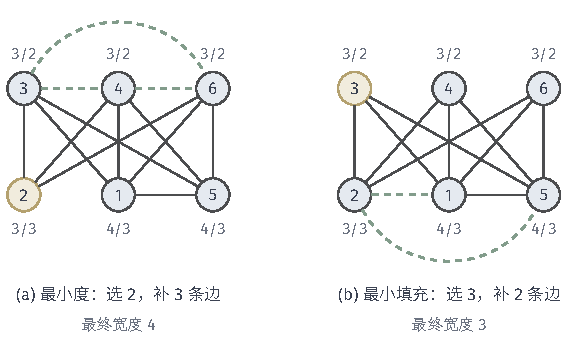
\includegraphics[width=96.778mm]{figures/01-basic-mathematics/04-graphs/tikz/c5-min-degree-min-fill/figure.pdf}
  \caption{最小度规则与最小填充规则的第一步。每个顶点旁的“$d/f$”是当前度数与当前缺边数。左：最小度规则在度数为$3$的顶点中按编号选$2$（黄色），要补三条绿色虚线，最终宽度为$4$。右：最小填充规则选缺边最少的$3$（黄色），只补两条边，最终宽度为$3$。}
  \label{fig:graph-dp-min-degree-min-fill}
\end{figure}

\paragraph{启发式只给出上界}
两种规则都只看一步：度数小不代表补边少，补边少也不保证以后的袋小。上例中最小度规则受平局规则影响，得到的宽度比最小填充多$1$；穷举全部$720$个消元次序可以核对，这个图上任何次序的诱导宽度都不小于$3$，所以最小填充在这里恰好达到了最好的次序。但换一个图，最小填充同样可能不是最优。因此报告结果时应分开写出构造的宽度、填充边数和结构操作次数，并把宽度理解为树宽的上界，而不是树宽本身。按算法~\ref{alg:graph-dp-greedy-order}的直接实现，每轮要为全部剩余顶点重算评分，最小填充一轮的检查量可达$\sum_v|N(v)|^2$；若用缓存只更新受补边影响的顶点，需要说明哪些边的增删会触发重算。

\subsection{弦图上的无填充消元}

\paragraph{单纯顶点与完美消元序}
填充边会使袋变大，最理想的情形是全程不需要补边。处理顶点$v$时不需要补边，当且仅当$v$的当前邻居已经两两相邻。当前邻居构成团的顶点称为\term{单纯顶点}（simplicial vertex）；没有邻居或只有一个邻居的顶点也算单纯顶点。若一个消元次序使每个顶点在被处理时都是当前图中的单纯顶点，就称它为\term{完美消元序}（perfect elimination ordering）。沿完美消元序消元不产生任何填充边，当前图始终是原图在剩余顶点上的诱导子图。

\paragraph{弦与弦图}
不是每个图都有完美消元序。四个顶点的环$1-2-3-4-1$中，每个顶点的两个邻居都不相邻：$1$与$3$的邻居都是$\{2,4\}$，缺边$\{2,4\}$；$2$与$4$的邻居都是$\{1,3\}$，缺边$\{1,3\}$。所以第一步就找不到单纯顶点。补入边$\{1,3\}$后，顶点$2$的邻居$\{1,3\}$相邻，可以先消去；剩下的三角形$1,3,4$中每个顶点都单纯，于是$(2,1,3,4)$是完美消元序。图~\ref{fig:graph-dp-chordal-four-cycle}画出了这一对比。

\begin{figure}[!htb]
  \centering
  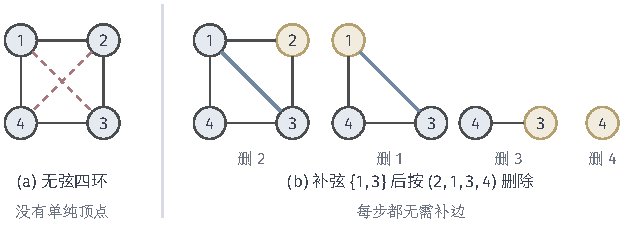
\includegraphics[width=106.306mm]{figures/01-basic-mathematics/04-graphs/tikz/c5-chordal-four-cycle/figure.pdf}
  \caption{无弦四环与补弦后的图。左：四环中每个顶点的两个邻居都不相邻（红色虚线为所缺的边），没有单纯顶点。右：补入弦$\{1,3\}$（蓝色）后，按$(2,1,3,4)$逐个删除，每一步被删除的黄色顶点的剩余邻居都已相邻，全程无填充。}
  \label{fig:graph-dp-chordal-four-cycle}
\end{figure}

四环的问题出在“长度至少为四而没有捷径的环”。在长度至少为$4$的环上，连接两个在环上不相邻的顶点的边称为该环的\term{弦}（chord）。每个长度至少为$4$的环都有弦的有限无向图称为\term{弦图}（chordal graph）。树没有环，是弦图；补入$\{1,3\}$后的四环是弦图；无弦四环不是。给一般图补边使之成为弦图称为\term{弦化}（chordal completion）。任何消元次序补边后的图都是弦图，因为该次序就是补边后图的完美消元序，由下面的定理即知；所以第一小节的构造实际上隐含了一次弦化。

\begin{theorem}[弦图与完美消元序]
\label{thm:graph-dp-chordal-peo}
有限无向图是弦图，当且仅当它有完美消元序。
\end{theorem}

\begin{proof}
先证有完美消元序的图是弦图。设图中有长度至少为$4$且无弦的环，考察环上最先被处理的顶点$v$。$v$在环上的两个邻居$u,w$此时都还在图中，并且与$v$相邻。$v$是单纯顶点，所以$u,w$相邻；而沿完美消元序处理时从不补边，$\{u,w\}$必是原图的边。环长至少为$4$，$u,w$在环上不相邻，于是$\{u,w\}$是这个环的弦，矛盾。

反方向的论证路线如下。第一步是一个引理：每个非空有限弦图都有单纯顶点，若它不是完全图，还有两个不相邻的单纯顶点。这一步需要分析极小分隔集，证明极小分隔集在弦图中都是团，本书不展开。第二步，弦图的诱导子图仍是弦图，因为诱导子图中的无弦环在原图中也无弦。于是可以反复删去一个单纯顶点，余下的图仍是弦图、仍有单纯顶点，直到删完，删除的次序就是完美消元序。
\end{proof}

\paragraph{构造与核验}
定理只说明弦图有完美消元序，并没有给出高效的求法。最直接的构造是逐次寻找单纯顶点：在当前图中按编号检查每个顶点，枚举它的每对邻居看是否相邻，找到第一个单纯顶点就删去它并追加到次序中；若非空的当前图中找不到单纯顶点，就报告输入不是弦图，并返回这个当前图作为证据，而不暗中补边。每轮最多检查$n$个顶点，检查顶点$v$需要$O(|N(v)|^2)$次查边，直接实现的总检查量最坏可达$O(n^4)$。存在线性时间的专门算法，这里不展开。

构造得到的次序应当独立核验。给定原图和一个次序，先确认它恰好包含每个顶点一次，再为每个顶点记下次序位置；对每个$v$取出原图中排在它之后的邻居，检查它们是否两两相邻。全部通过时次序是完美消元序，因为在不补边的前提下，处理$v$时的当前邻居恰好就是这些后续邻居；发现缺边时，就把$v$和那对不相邻的邻居作为失败证据返回。核验的检查量为$O(n+m)$再加$\sum_v|N^+_\pi(v)|^2$次查边。例如把$(2,1,3,4)$用于无弦四环，第一个顶点$2$的后续邻居$\{1,3\}$不相邻，立即被拒绝；用于补弦后的图则通过。

\paragraph{极大团与最大团}
弦图上可以直接用团作袋，这需要区分两种“最大”。不能再加入任何其他顶点而保持两两相邻的团称为\term{极大团}（maximal clique），这是按集合包含判断的；在所有团中顶点数最多的称为\term{最大团}（maximum clique）。例如三角形$1,2,3$外加一条边$\{3,4\}$，极大团是$\{1,2,3\}$和$\{3,4\}$；后者不能再扩大，但只有两个顶点，不是最大团。下面的团树需要全部极大团，而不只是最大的几个。

\subsection{团树的构造}

以弦图的全部极大团为袋、并满足运行交集的树分解称为\term{团树}（junction tree，也称clique tree）。团树中每个袋都是团，没有因填充而多出的变量，相邻两袋的交集就是它们共享的变量。本小节回答两个问题：怎样从完美消元序得到全部极大团；怎样把它们连成满足运行交集的树。

\paragraph{从完美消元序得到极大团}
设$\pi$是已经核验的完美消元序。对每个顶点$v$，候选集合$K_v=\{v\}\cup N^+_\pi(v)$是团，因为$v$被处理时是单纯顶点。反过来，任一团$C$都包含在某个$K_v$中：取$C$中最先被处理的顶点$v$，$C$的其余顶点都在$v$之后且与$v$相邻，所以都属于$N^+_\pi(v)$。因此极大团恰好是候选集合中不被其他候选严格包含的那些。具体做法是：生成全部$K_v$，删去重复的集合，再删去被其他候选严格包含的集合。

图~\ref{fig:graph-dp-clique-tree-mst}的弦图有边$\{1,2\},\allowbreak\{1,3\},\allowbreak\{2,3\},\allowbreak\{2,4\},\allowbreak\{3,4\},\allowbreak\{3,5\},\allowbreak\{4,5\}$，$(1,2,5,3,4)$是它的完美消元序。候选集合为$K_1=\{1,2,3\}$、$K_2=\{2,3,4\}$、$K_5=\{3,4,5\}$、$K_3=\{3,4\}$、$K_4=\{4\}$；删去被包含的$K_3,K_4$，得到三个极大团$A=\{1,2,3\}$、$B=\{2,3,4\}$、$C=\{3,4,5\}$。

\paragraph{用最大权生成树连接}
直觉上，共享变量多的团应该相邻，这样接口才能携带足够的共同变量。在以极大团为顶点的完全图上，给每对团$C,D$赋权$w(C,D)=|C\cap D|$，交集为空的零权边也保留；然后求这个图的最大权生成树，可以把权取负后调用第~\ref{sec:graph-minimum-spanning-tree}节的Kruskal或Prim方法。上例中$w(A,B)=2$、$w(B,C)=2$、$w(A,C)=1$，最大权生成树是$A-B-C$，总权为$4$。若改选$A-B$与$A-C$，总权为$3$，此时含$4$的两个团$B,C$之间隔着不含$4$的$A$，运行交集被破坏，如图~\ref{fig:graph-dp-clique-tree-mst}右侧所示。

\begin{figure}[!htb]
  \centering
  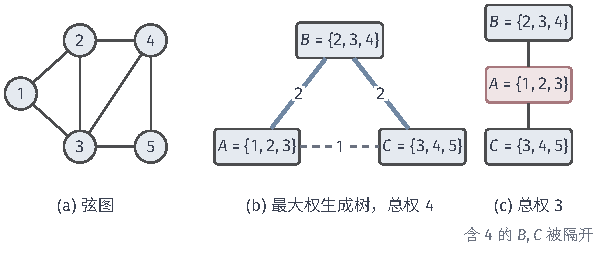
\includegraphics[width=102.306mm]{figures/01-basic-mathematics/04-graphs/tikz/c5-clique-tree-mst/figure.pdf}
  \caption{用交集权重的最大权生成树连接极大团。左：弦图。中：三个极大团组成的候选完全图，边上的数是交集大小，蓝色粗线是总权为$4$的最大权生成树$A-B-C$，虚线是未被选中的候选边。右：总权为$3$的另一棵生成树$B-A-C$，含$4$的团$B,C$被不含$4$的$A$（红色）隔开，不满足运行交集。}
  \label{fig:graph-dp-clique-tree-mst}
\end{figure}

下面的定理说明，这个例子中的对应关系是一般的。

\begin{theorem}[团树与最大权生成树]
\label{thm:graph-dp-clique-tree-mst}
设$\mathcal H$是非空有限弦图，$\mathcal C$是它的全部极大团。在以$\mathcal C$为顶点的完全图上令$w(C,D)=|C\cap D|$。则一棵生成树满足运行交集，当且仅当它的总权最大。
\end{theorem}

\begin{proof}
先给出任意生成树的总权上界。对生成树$\mathcal T'$，把每条边的权按共享变量拆开计数：
\[
\sum_{\{C,D\}\in\mathcal T'}|C\cap D|=\sum_{v}e_v,
\]
其中$e_v$是两端都含$v$的树边条数。设$v$属于$r_v$个极大团，两端都含$v$的树边正是$\mathcal T'$在这$r_v$个节点上的诱导子图的边；树的诱导子图没有环，是$r_v$个节点上的森林，所以$e_v\leq r_v-1$，且等号成立当且仅当这个诱导子图连通，即含$v$的团在$\mathcal T'$中连通。于是总权不超过$\sum_v(r_v-1)$，等号成立当且仅当对每个$v$都满足运行交集。

剩下要证明确实存在满足运行交集的生成树，即团树存在；那时最大总权恰为$\sum_v(r_v-1)$，最大权生成树就是满足运行交集的生成树。取一个完美消元序，按定理~\ref{thm:graph-dp-elimination-decomposition}的方法以$K_v$为袋得到树分解。若某个袋包含于相邻的袋，就把这条袋树边收缩，只保留较大的袋：顶点覆盖和边覆盖不受影响；对运行交集，被收缩的较小袋中的变量都在较大袋中，收缩一条两端都含$v$的边不破坏$T_v$的连通性，而不含$v$的较小袋本来不在$T_v$中，收缩后$T_v$也不变。反复收缩，直到没有相邻两袋有包含关系。这时任何两个袋都没有包含关系：若$B_s\subseteq B_t$而$s,t$不相邻，取路径上与$s$相邻的节点$s'$，由运行交集$B_s$的每个变量都在$B_{s'}$中，与“相邻袋无包含关系”矛盾。各袋都是团且互不包含；每个极大团都被某个袋容纳（引理~\ref{lem:graph-dp-clique-in-bag}），而袋本身是团，所以二者相等；每个袋也都是某个极大团，否则它会被那个极大团所在的另一个袋严格包含。于是剩下的袋恰好是全部极大团，各出现一次，团树存在。
\end{proof}

在上例中，$r_1=1$、$r_2=2$、$r_3=3$、$r_4=2$、$r_5=1$，上界$\sum_v(r_v-1)=4$，正好等于$A-B-C$的总权。不连通的弦图中，不同分量的团之间交集为空，零权边只用于把各分量的团树连成一棵树，不影响上界。

\paragraph{适用范围与结果核对}
定理要求输入是弦图，并且使用全部极大团。对无弦四环，极大团是四条边$\{1,2\},\allowbreak\{2,3\},\allowbreak\{3,4\},\allowbreak\{1,4\}$，每个顶点属于两个团；要让每个顶点的两个团相邻，需要四条树边，而四个节点的树只有三条边，所以任何生成树都不满足运行交集。一般图应先弦化，例如用某个消元次序补边，再在弦化后的图上构造团树；在原图的极大团上任选一棵树并不能保证得到树分解。选哪一种弦化决定了袋的大小，而团树构造只负责连接给定弦图的团，不负责找最好的弦化。

最大权生成树依赖上面的定理才保证运行交集，因此输出后仍应逐个顶点检查含它的团是否连通，作为对输入是否为弦图、团列表是否完整的独立核对。开销方面，设极大团有$p$个，候选完全图有$p(p-1)/2$条边，每条边的权需要一次集合求交；排序与并查集的开销按第~\ref{sec:graph-minimum-spanning-tree}节的分析计算。弦图的极大团数不超过顶点数$n$，因为每个极大团都是某个$K_v$。

% 第5章第6节：树分解上的动态规划（局部函数的分配、接口表与袋消息、配置恢复与开销、计数与加权求和、半环）。

\section{树分解上的动态规划}
\label{sec:graph-bag-dp}

有了一个已经核验的树分解，就可以把第~\ref{sec:graph-tree-dp}节树上的递推搬到袋组成的树上：原来每个顶点是一个变量，现在每个节点是一组变量；原来消息以单个接收变量为索引，现在以相邻两袋的接口为索引。本节先说明局部函数怎样分配到袋中，再给出袋之间的消息递推及其正确性，然后讨论配置恢复和计算开销；最后保持同样的结构，把“相加后取最小”换成其他运算，得到可行配置计数和加权求和。

本节的例子仍是四变量问题：树分解有两个节点$s,t$，袋为$B_s=\{1,2,3\}$与$B_t=\{2,3,4\}$，接口为$\{2,3\}$；局部函数$\phi_A,\phi_B$由表~\ref{tab:graph-dp-ternary-tables}给出。

\subsection{局部函数的分配}

\paragraph{每个函数恰好归入一个袋}
计算前先把每个局部函数$\phi_a$归入一个袋$B_{\alpha(a)}$，要求$S_a\subseteq B_{\alpha(a)}$；由引理~\ref{lem:graph-dp-clique-in-bag}，这样的袋总存在。每个函数只归入一次。节点$t$上全部归入函数之和称为袋成本：
\begin{equation}
\Phi_t(\bm x_{B_t})=\sum_{a:\,\alpha(a)=t}\phi_a(\bm x_{S_a}),
\label{eq:graph-dp-bag-cost}
\end{equation}
没有函数归入的袋取$\Phi_t\equiv0$，但仍保留袋中的变量，因为它们可能需要经过这个袋来保持一致。在例子中，$\phi_A$只能归入$B_s$，$\phi_B$只能归入$B_t$，于是$\Phi_s=\phi_A$、$\Phi_t=\phi_B$。

只归入一次是数值正确性的要求，不是结构上的要求。设问题中另有一个成对项$\phi_{2,3}(x_2,x_3)$，它的作用域同时被$B_s$和$B_t$包含，归入哪个袋都可以；但若两边各计一次，最后得到的就是$F+\phi_{2,3}$的最小值，而不是$F$的最小值。共享变量可以在多个袋中重复出现，同一个成本项却不能在多处重复累计。

\paragraph{分配清单的核对}
计算前可以对照一份分配清单逐项检查：每个局部函数都有归属，没有遗漏；没有函数被归入两个袋；每个函数的作用域确实包含在所归入的袋中。树分解的三个条件只保证有地方容纳每个函数，这份唯一归属则保证每一项成本恰好计算一次。袋之间的交集只说明哪些变量需要协调，它本身不对应任何成本，不能当作额外的局部函数加入。

\subsection{接口表与消息递推}

\paragraph{袋之间的消息}
设节点$s,t$在袋树中相邻，接口为$S_{s,t}=B_s\cap B_t$。从$s$发往$t$的消息是一张以接口变量为索引的表：固定接口取值后，把袋成本与$s$从其他邻居收到的消息相加，再对$B_s$中不属于接口的变量取最小，
\begin{equation}
\mu_{s\to t}(\bm x_{S_{s,t}})=\min_{\bm x_{B_s\setminus S_{s,t}}}\Bigl[\Phi_s(\bm x_{B_s})+\sum_{r\in N(s)\setminus\{t\}}\mu_{r\to s}(\bm x_{S_{r,s}})\Bigr],
\label{eq:graph-dp-bag-message}
\end{equation}
其中$N(s)$是$s$在袋树中的邻居。这与式~\eqref{eq:graph-dp-tree-message}的结构相同，只是被汇总的不再是单个变量，而是袋内的非接口变量。

在例子中，$s$是叶节点，它的非接口变量只有$x_1$，所以
\[
\mu_{s\to t}(x_2,x_3)=\min_{x_1}\phi_A(x_1,x_2,x_3).
\]
图~\ref{fig:graph-dp-bag-message-table}逐行列出了这张四项表：接口取值为$00,01,10,11$时，消息值依次为$0,0,1,2$，达到最小值的$x_1$依次为$1,0,1,1$。它与上一节消去$x_1$得到的$\psi_1$相同。$x_1$已经被汇总，不再出现在表中；$x_2,x_3$作为接口仍然显式保留，右袋读取这张表时要按同样的$(x_2,x_3)$取值对齐。

\begin{figure}[!htb]
  \centering
  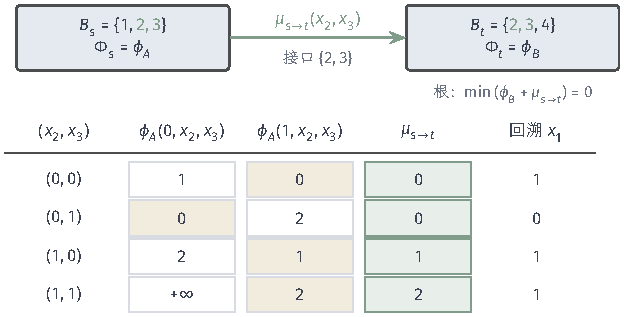
\includegraphics[width=105.650mm]{figures/01-basic-mathematics/04-graphs/tikz/c5-bag-message-table/figure.pdf}
  \caption{两袋之间的消息。左袋$B_s=\{1,2,3\}$只含$\phi_A$，右袋$B_t=\{2,3,4\}$只含$\phi_B$，接口为$\{2,3\}$（绿色）。下方表格对接口的每种取值比较$x_1=0,1$两个候选，取较小者作为消息值，黄色格是被选中的候选；绿色列是消息值，最后一列是回溯表。根袋$B_t$把消息与$\phi_B$相加后对$x_2,x_3,x_4$取最小，得到最优值$0$。}
  \label{fig:graph-dp-bag-message-table}
\end{figure}

选$t$为根，根处合并袋成本与全部入消息，再对根袋的全部变量取最小：
\[
\min_{x_2,x_3,x_4}\bigl[\phi_B(x_2,x_3,x_4)+\mu_{s\to t}(x_2,x_3)\bigr]=0,
\]
在$(x_2,x_3,x_4)=(0,1,0)$处达到，因为$\phi_B(0,1,0)=0$且$\mu_{s\to t}(0,1)=0$，而所有值都非负。一般情形下按后序计算：每个节点收齐子节点的消息后向父节点发送消息，最后在根处合并。

\paragraph{为什么沿袋树计算是正确的}
树上消息的正确性依赖于一件事：删去一条边后，两侧除了接收变量以外没有共同的变量。袋树上，这件事由运行交集保证。删去袋树边$\{s,t\}$后，袋树分成两部分；记$s$一侧全部袋中出现的变量为$V_{s|t}$，$t$一侧为$V_{t|s}$。若某个变量$v$在两侧都出现，从它在$s$侧的某个出现位置到$t$侧的某个出现位置，袋树路径必须经过边$\{s,t\}$，由运行交集，$B_s$与$B_t$都含$v$。所以
\begin{equation}
V_{s|t}\cap V_{t|s}\subseteq S_{s,t},
\label{eq:graph-dp-interface-separation}
\end{equation}
即接口把两侧的变量隔开：固定接口取值后，两侧的其余变量互不重叠，可以分别求最小。

\begin{theorem}[袋消息的含义]
\label{thm:graph-dp-bag-message}
设$(\mathcal T,\{B_t\}_{t\in T})$是原始图的树分解，每个局部函数恰好归入一个包含其作用域的袋。对袋树的边$\{s,t\}$，记$A_{s|t}$为归入$s$一侧各袋的局部函数。则对每个接口取值$\bm x_{S_{s,t}}$，
\[
\mu_{s\to t}(\bm x_{S_{s,t}})=\min_{\bm x_{V_{s|t}\setminus S_{s,t}}}\ \sum_{a\in A_{s|t}}\phi_a(\bm x_{S_a}).
\]
进一步，对任意根节点$\rho$，$\min_{\bm x}F(\bm x)=\min_{\bm x_{B_\rho}}\bigl[\Phi_\rho+\sum_{r\in N(\rho)}\mu_{r\to\rho}\bigr]$。
\end{theorem}

\begin{proof}
对$s$一侧的节点数归纳。设$s$在$t$以外的邻居为$r_1,\ldots,r_k$（叶节点时$k=0$）。删去$s$后，$s$一侧的其余节点分成$r_1,\ldots,r_k$各自的一侧。由式~\eqref{eq:graph-dp-interface-separation}应用于边$\{r_j,s\}$，$V_{r_j|s}$与$B_s$的公共变量都在$S_{r_j,s}$中；不同的$r_j,r_l$两侧若有公共变量，它在袋树上的两个出现位置之间的路径经过$s$，所以也在$B_s$中。因此集合
\[
B_s\setminus S_{s,t},\qquad V_{r_1|s}\setminus B_s,\qquad\ldots,\qquad V_{r_k|s}\setminus B_s
\]
两两不交，它们的并恰为$V_{s|t}\setminus S_{s,t}$。另一方面，$A_{s|t}$按函数归入的节点分为归入$s$的部分和归入各$r_j$一侧的部分$A_{r_j|s}$，每个函数恰在一处；$A_{r_j|s}$中函数的变量都在$V_{r_j|s}$中，其中属于$B_s$的部分又在$S_{r_j,s}$中。

现在固定$\bm x_{B_s}$。各$A_{r_j|s}$中函数之和只依赖$\bm x_{S_{r_j,s}}$与互不相交的变量组$\bm x_{V_{r_j|s}\setminus B_s}$，按式~\eqref{eq:graph-dp-min-rules}后的第三条规则可以分别求最小，由归纳假设，第$j$项的最小值为$\mu_{r_j\to s}(\bm x_{S_{r_j,s}})$。再对$\bm x_{B_s\setminus S_{s,t}}$求最小值，就得到式~\eqref{eq:graph-dp-bag-message}。根处的等式用同样的拆分得到：由顶点覆盖，全部变量是$B_\rho$与各$V_{r|\rho}\setminus B_\rho$的不交并，全部函数分为归入$\rho$的与归入各邻居一侧的。
\end{proof}

证明用到了三项条件：运行交集保证接口隔开两侧；顶点覆盖保证根处的汇总涉及全部变量；每个函数恰好归入一个袋，保证每一项只计一次。少了任何一项，递推得到的数都可能不等于原问题的最小值。

\subsection{配置恢复与计算开销}

\paragraph{沿袋树回溯}
计算$\mu_{s\to t}$时，对每个接口取值同时记录达到最小值的非接口变量取值$\beta_{s\to t}(\bm x_{S_{s,t}})$，即袋上的回溯表。根处取使合并值最小的$\bm x_{B_\rho}$，然后按前序：对已确定全部变量的节点$t$及其子节点$s$，令$\bm x_{B_s\setminus S_{s,t}}=\beta_{s\to t}(\bm x_{S_{s,t}})$。$B_s$中属于接口的变量此前已在$B_t$中取定；不属于接口的变量由运行交集不会出现在$s$一侧以外，因而此前没有被赋值。所以每个变量恰好被赋值一次，在它出现的所有袋中取同一个值。

例子中根取$(x_2,x_3,x_4)=(0,1,0)$，查左袋的回溯表得$\beta_{s\to t}(0,1)=0$，即$x_1=0$。恢复的配置$(0,0,1,0)$代回原始局部函数得$\phi_A(0,0,1)+\phi_B(0,1,0)=0+0=0$，与最优值一致，也与第~\ref{sec:graph-variable-elimination}节两种消元次序的结果相同。若根处的最小值为$+\infty$，则报告没有可行配置。

\paragraph{时间与存储}
设袋树有$N$个节点，宽度为$k$，各变量至多$q$个状态。计算$\mu_{s\to t}$时要枚举$\bm x_{B_s}$的至多$q^{k+1}$种取值，每种取值读取归入$s$的各函数一次、读取$s$的其他入消息各一次，所以全部向上消息的时间约为
\[
\sum_{s}\bigl(|A_s|+|N(s)|\bigr)q^{k+1}=O\bigl((|A|+N)\,q^{k+1}\bigr),
\]
其中$|A_s|$是归入$s$的函数个数，并用到了袋树中$\sum_s|N(s)|=2(N-1)$。每张消息表与回溯表各有$\prod_{i\in S_{s,t}}|\mathcal X_i|\leq q^{k}$项。若还需要每个袋上各取值的最小总成本，就像树上那样再按前序发送一遍反向消息，时间与存储加倍。

这里的计算是精确的，但精确不等于便宜。宽度$k$出现在指数上，$q=10$、$k=10$时一张袋表就有$10^{11}$项；若查询要求保留很多变量的联合最小成本表，输出本身也可能大得不可承受。另外，本节的正确性证明依赖袋树无环和运行交集。若直接在带环的原始图上按式~\eqref{eq:graph-dp-tree-message}反复交换消息，同一部分成本会沿环被重复计入，上面的证明不再适用；这类迭代是否收敛、收敛到什么，需要另外分析，留到后续推断部分。

\subsection{计数与有限加权求和}

\paragraph{换一种组合与汇总}
保持同样的局部结构和袋树，可以回答另外两个问题。第一个问题是：有多少个可行配置？把每个局部函数换成可行性指示$\mathbb I\{\phi_a(\bm x_{S_a})<+\infty\}$，一个配置可行当且仅当这些指示全为$1$，即它们的乘积为$1$；于是可行配置数为$\sum_{\bm x}\prod_a\mathbb I\{\phi_a<+\infty\}$。第二个问题是：给每个局部函数一张非负权重表$w_a(\bm x_{S_a})$，把配置的权重定义为各局部权重之积，求全部配置的权重总和$\sum_{\bm x}\prod_a w_a(\bm x_{S_a})$。两者都把“局部项相加、对变量取最小”换成“局部项相乘、对变量求和”。

推导与最小成本完全平行。式~\eqref{eq:graph-dp-min-rules}中的三条规则换成：有限求和可以分步进行；与求和变量无关的因子可以提到求和号外，即$\sum_y c\,g(y)=c\sum_y g(y)$；互不相交的变量组上，乘积之和等于和之积。于是把式~\eqref{eq:graph-dp-bag-message}中的加号换成乘号、最小化换成求和，消息就变成“$s$一侧的可行配置数”或“$s$一侧的权重总和”，以接口取值为索引。

表~\ref{tab:graph-dp-weights}给出四变量例子的权重表，权重恰在禁止的组合处为$0$。表~\ref{tab:graph-dp-three-aggregations}对接口的每种取值并列三种任务的左袋消息和右袋汇总值，最后一行是根处的结果：最小成本为$0$，可行配置有$10$个，权重总和为$19$。逐一枚举$16$个配置可以核对这三个数。

\begin{table}[!htb]
  \centering
  \caption{四变量例子的非负局部权重。第一列的三位二进制串对$w_A$表示$(x_1,x_2,x_3)$，对$w_B$表示$(x_2,x_3,x_4)$；权重为$0$的位置恰是表~\ref{tab:graph-dp-ternary-tables}中成本为$+\infty$的位置。}
  \label{tab:graph-dp-weights}
  \begin{tabular}{ccccccccc}
    \toprule
    取值 & $000$ & $001$ & $010$ & $011$ & $100$ & $101$ & $110$ & $111$\\
    \midrule
    $w_A$ & $1$ & $2$ & $1$ & $0$ & $2$ & $1$ & $1$ & $1$\\
    $w_B$ & $1$ & $1$ & $2$ & $0$ & $0$ & $2$ & $1$ & $2$\\
    \bottomrule
  \end{tabular}
\end{table}

\begin{table}[!htb]
  \centering
  \caption{三种任务在同一接口上的消息。最小成本使用$\min$与$+$，可行计数与加权总和使用$\sum$与$\times$。“左”列是从$B_s$发出的消息，对$x_1$汇总；“右”列是$B_t$对$x_4$的汇总；根处对每个接口取值组合两列（最小成本相加，其余相乘），再对接口汇总（最小成本取最小，其余求和）。}
  \label{tab:graph-dp-three-aggregations}
  \begin{tabular}{ccccccc}
    \toprule
    & \multicolumn{2}{c}{最小成本} & \multicolumn{2}{c}{可行计数} & \multicolumn{2}{c}{加权总和}\\
    \cmidrule(lr){2-3}\cmidrule(lr){4-5}\cmidrule(lr){6-7}
    $(x_2,x_3)$ & 左 & 右 & 左 & 右 & 左 & 右\\
    \midrule
    $(0,0)$ & $0$ & $1$ & $2$ & $2$ & $3$ & $2$\\
    $(0,1)$ & $0$ & $0$ & $2$ & $1$ & $3$ & $2$\\
    $(1,0)$ & $1$ & $0$ & $2$ & $1$ & $2$ & $2$\\
    $(1,1)$ & $2$ & $1$ & $1$ & $2$ & $1$ & $3$\\
    \midrule
    根处 & \multicolumn{2}{c}{$\min(1,0,1,3)=0$} & \multicolumn{2}{c}{$4+2+2+2=10$} & \multicolumn{2}{c}{$6+6+4+3=19$}\\
    \bottomrule
  \end{tabular}
\end{table}

三种任务的输出含义不同。最小成本是一个配置的值，还可以回溯出达到它的配置；计数和加权总和是对全部配置的汇总，没有“达到它的配置”可言。例如接口取$(1,1)$时，左袋的最小成本消息为$2$，计数消息为$1$，因为$x_1=0$的那一行被禁止，只剩$x_1=1$一个可行选择；加权消息为$0+1=1$。

\paragraph{半环与分配律}
上面三种任务共用同一套递推，是因为它们的运算满足同样的代数规则。设集合$\mathcal S$上有两种运算：$\oplus$用于跨不同取值的汇总，$\otimes$用于在一个配置内组合各局部项。若两种运算都满足结合律和交换律，各有单位元$\bar0$与$\bar1$，满足$\bar0\otimes a=\bar0$，并且$\otimes$对$\oplus$满足分配律
\[
a\otimes(b\oplus c)=(a\otimes b)\oplus(a\otimes c),
\]
就称$(\mathcal S,\allowbreak\oplus,\allowbreak\otimes,\allowbreak\bar0,\allowbreak\bar1)$为交换\term{半环}（semiring）。最小成本对应$(\mathbb R\cup\{+\infty\},\allowbreak\min,\allowbreak+,\allowbreak+\infty,\allowbreak0)$，此时分配律就是$a+\min(b,c)=\min(a+b,a+c)$；计数对应自然数上的$(+,\times,0,1)$；加权求和对应非负实数上的$(+,\times,0,1)$；只判断是否存在可行配置时，还可以用布尔值上的“或”与“且”。把变量消元和袋消息中的$\min$换成$\oplus$、$+$换成$\otimes$，前面的正确性证明逐字成立，因为证明只用到了结合律、交换律和分配律。半环不要求减法或除法。

\paragraph{不能随意交换的汇总}
分配律只保证同一种汇总可以分步、移项。若一个问题对一部分变量取最大值、对另一部分变量求和，两种汇总一般不能交换次序。例如对表$h(x,y)$，$h(0,0)=h(1,1)=4$、$h(0,1)=h(1,0)=0$，有
\[
\max_x\sum_y h(x,y)=4,\qquad \sum_y\max_x h(x,y)=8 .
\]
前者要求所有$y$共用同一个$x$，后者允许$x$随$y$改变。这类混合问题只能按限定的次序消元，所需的中间表可能比单一汇总时大。把非负权重归一化为概率还要求总和为正且有限；这些概率解释、边缘化查询以及带环图上的近似消息方法，都留到后续推断部分。

% 第5章第7节：本章小结。

\section{本章小结}
\label{sec:graph-dp-summary}

本章处理的问题由局部函数组成：每个变量取有限个状态，整体成本是若干局部项之和，每一项只读取少数变量。计算的核心始终是同一个动作：固定一组接口变量，把只在一侧出现的变量汇总掉，留下一张以接口为索引的表。链上，接口是一个变量，表沿链逐个传递；树上，接口仍是一个变量，但一个顶点要合并多棵子树传来的消息；一般依赖图上，变量消元按任意次序逐个汇总变量，正确性不变，中间表的作用域却随次序变化。树分解把这些同时处理的变量组织成袋树，消元次序可以机械地产生树分解，弦图上还能用极大团和最大权生成树得到团树；最后，袋上的消息把树上的递推推广到一般图。

这些步骤中有三种不能互相替代的对象。局部函数表记录数值，决定消息的具体取值；原始图记录哪些变量共同出现，决定消元时的填充边和袋必须容纳的团；袋树记录计算的组织方式，决定消息沿什么路径传递、以什么为索引。原始图不能恢复函数表，袋树的边也不是原始图的边；混淆它们会导致把高阶约束错拆成成对规则，或在袋之间重复累计成本。

精确计算依赖一组明确的条件：局部函数给出完整的作用域；状态集合有限；组合与汇总的运算满足结合律、交换律与分配律，即构成半环；每个局部函数恰好归入一个包含其作用域的袋；袋树满足运行交集，使接口把两侧的变量隔开。计算规模则主要由袋的大小控制，宽度为$k$、每个变量至多$q$个状态时，袋表至多$q^{k+1}$项。树宽小的图上精确计算可行，树宽大的图上同样的方法仍然正确，但可能无法承受。后续的概率模型会把这些表解释为未归一化的概率、把求和解释为边缘化，但归一化条件、查询中不同汇总的次序以及带环图上的近似方法，都需要在那里另外说明，不能由本章的结论直接推出。

本章比较的是有限配置：每个变量取离散的状态，目标是在所有配置中找最小值或求汇总。下一章转向另一类任务：顶点上的数值已经给定，要研究它们沿边怎样变化，怎样通过图上的线性算子对它们进行变换和滤波，并据此划分图。所需的工具也随之改变，从有限比较与递推转向内积、二次型和第三部分的谱分解。


\chapter{图上的谱方法}
\label{chap:graph-spectral}

设想一张传感器网络：每个顶点是一处测点，读数是一个实数，边表示哪些测点相邻并应当相互比较。拿到一组读数后，常会提出三个问题：这组数值沿边变化得剧烈还是平缓？能否压低读数中逐点跳动的成分，保留整体趋势？能否依据连接强弱，把测点分成内部联系紧、彼此联系松的两组？前五章处理的是路径、流、子集和有限配置这类离散对象；本章的对象换成了挂在顶点上的数值，所用工具也随之换成第三部分建立的有限维线性代数：内积、二次型和实对称矩阵的谱分解。

前三节构造需要的图算子。第~\ref{sec:graph-vertex-edge-functions}节区分顶点上的数值与边上的数值，并用关联矩阵计算沿边差分。第~\ref{sec:graph-laplacian}节从“读取邻居并比较”和“取边差、按边权缩放、汇总回顶点”两条路线得到同一个组合拉普拉斯，其二次型累计各边差值的平方，用来衡量沿边变化。第~\ref{sec:graph-normalized-laplacian}节处理各顶点连接总量不等的情形，引入度加权内积，得到对称归一化和随机游走两种归一化拉普拉斯，并说明它们的差别在于坐标与内积。

后四节利用这些算子的谱。第~\ref{sec:graph-spectrum-connectivity}节说明特征向量按沿边变化从小到大排列，零特征值的重数等于正权连通分量的个数，归一化后的谱落在$[0,2]$中。第~\ref{sec:graph-fourier-transform}节把顶点函数展开在特征基上，得到图傅里叶变换；在环图上，这组基正是熟悉的复指数。第~\ref{sec:graph-filtering}节逐个模态调节系数，从而改变函数本身，并比较显式谱分解与只需稀疏乘法的多项式实现。第~\ref{sec:graph-spectral-partition}节把两组划分写成二次型的最小化，放宽取值限制后由第二特征向量得到下界和候选分组。

全章约定图有限、无向、无自环，边权非负且对称。允许零权的结构边存在，但能量、零空间和谱的结论只由正权边决定。真正的有向图和带负权的图不能直接套用本章的对称谱结论。特征值一律按从小到大编号，这与第~\ref{sec:ls-spectral-theory}节按从大到小排列的习惯相反：在图上，小特征值对应平缓的变化，从它们数起更方便。

% 第6章第1节：顶点函数与边函数（顶点函数、边函数、沿边差分）。

\section{顶点函数与边函数}
\label{sec:graph-vertex-edge-functions}

谱方法处理的是挂在图上的数值。动手构造算子之前，先要说清三件事：数值放在哪里（顶点还是边），取什么值，允许做哪些运算。本节先分别建立顶点函数与边函数，再用关联矩阵实现从前者到后者的沿边差分。矩阵在这里只负责实现已经说明的作用，不代替对象本身的解释。

\subsection{顶点函数}
\label{sec:graph-spec-vertex-functions}

回到章首的传感器网络。每个测点给出一个温度读数，相当于给每个顶点指定一个实数，也就是一个映射$f:V\to\mathbb R$，称为\term{顶点函数}（vertex function），也常称为\term{图信号}（graph signal）。固定顶点的一个编号$V=\{1,\ldots,n\}$后，顶点函数可以存成向量$\bm f=(f_1,\ldots,f_n)^{\top}\in\mathbb R^n$，其中$f_i=f(i)$。全体顶点函数于是构成$n$维实向量空间：两个函数可以逐点相加、数乘，即$(\alpha\bm f+\beta\bm g)_i=\alpha f_i+\beta g_i$；也可以使用欧氏内积$\langle\bm f,\bm g\rangle=\sum_if_ig_i$和长度$\lVert\bm f\rVert_2$（第~\ref{sec:ls-inner-product-definition}节）。

编号只决定数值在数组中的位置，不改变数值属于哪个顶点。换一种编号，相当于用置换矩阵$\bm P$重排坐标，得到$\bm P\bm f$；第~\ref{sec:graph-isomorphism}节已经说明，邻接矩阵在重编号下同步变为$\bm P\bm A\bm P^{\top}$。本章后面的每个算子都要检查这一点：重编号后输出也只是随之重排，不能因为编号不同而改变结果。

并非所有挂在顶点上的数字都能这样运算。给顶点按类别标上$1,2,3$时，这些数字首先表示身份，“$1$号类与$3$号类的平均是$2$号类”没有意义，也不能把类别编号当温度求平均。处理类别标记的是第~\ref{sec:graph-wl-refinement}节的标记细化，它只比较相同与否和出现次数；本章只处理确实可以相加、数乘的数值。

一个测点有时同时记录温度、湿度等多个读数，可以把$c$个通道按列排成矩阵$\bm X\in\mathbb R^{n\times c}$。本章的节点算子都是$n\times n$矩阵，左乘$\bm X$时对每一列分别作用，各通道之间互不干扰；若要把不同通道混合，需要右乘一个$c\times c$矩阵，这是另一项操作，不属于图的结构。下文只讨论单个通道。

\subsection{边函数}
\label{sec:graph-spec-edge-functions}

数值也可以挂在边上：管道中的流量、两端读数之差、相邻两点间的作用量，都以边为索引。给每条边指定一个实数的映射$\varphi:E\to\mathbb R$称为\term{边函数}（edge function）；固定边的编号$e_1,\ldots,e_m$后，它存成$\bm\varphi\in\mathbb R^m$。与顶点函数一样，边函数也可以逐边相加、数乘，并带有欧氏内积。

无向边本身没有方向，但许多边上的数值带有符号。说“沿边$\{1,2\}$的流量是$3$”时，必须说明是从$1$流向$2$还是反过来；从$2$流向$1$的流量$3$，等于从$1$流向$2$的流量$-3$。因此记录有符号的边上数值之前，要给每条无向边选一个参考方向。这个方向只是记账约定：把某条边的参考方向反过来，对应的数值改变符号，所描述的物理量不变。这与有向图中弧的方向不同，后者属于图的结构，不能随意翻转。

无向边权是另一种情形。权$w_{i,j}=w_{j,i}\geq0$描述两端应当被比较的强度，不随方向改变符号，可以直接看成无向边上的函数。权与流量、差值的区别还在于计算中的角色：本章的算子把边权当作固定参数，把边差、流量这类量当作待处理的数值。以三点路径$1-2-3$为例，顶点函数是$\mathbb R^3$中的向量，边函数是$\mathbb R^2$中的向量；二者维数不同、索引不同，不能相加。

边权为零的结构边仍然属于边集$E$，第~\ref{chap:graph-traversal}、\ref{chap:graph-optimization}章的遍历与组合优化是否使用它，由那些问题自己的规则决定。本章的算子只受正权边影响，所以把它们单独收集起来：
\[
 E_+=\bigl\{\{i,j\}\in E:w_{i,j}>0\bigr\},
\]
称$(V,E_+)$为\term{正权支撑}图（positive-weight support graph），记$m_+=|E_+|$。按顶点编号把权排成对称矩阵$\bm W=[w_{i,j}]$，没有边的位置记$0$；按边编号把权排成对角矩阵$\bm W_E=\operatorname{diag}(w_{e_1},\ldots,w_{e_m})$。注意$\bm W$中的$0$不区分“无边”与“零权边”，需要区分时另存结构掩码（第~\ref{sec:graph-representations}节）。

\subsection{沿边差分}
\label{sec:graph-spec-edge-differences}

顶点函数最基本的沿边信息是每条边两端的差。第~\ref{sec:graph-representations}节的关联矩阵正好用来计算它：给每条无向边选定参考方向后，$\bm B\in\mathbb R^{n\times m}$的第$e$列在起点处为$1$、终点处为$-1$，其余为零。若边$e$从$i$指向$j$，则
\begin{equation}
 (\bm B^{\top}\bm f)_e=f_i-f_j .
 \label{eq:graph-spec-edge-difference}
\end{equation}
$\bm B^{\top}$把顶点函数映成边函数，记录每条边上“起点减终点”的差。由于$\bm B$的每一列恰有一个$1$和一个$-1$，常量函数$\bm1$的每条边差都为零：$\bm B^{\top}\bm1=\bm0$。

以三点路径为例，取参考方向$e_1:1\to2$、$e_2:2\to3$，顶点值$\bm f=(3,1,2)^{\top}$。此时
\[
 \bm B=\begin{bmatrix}1&0\\-1&1\\0&-1\end{bmatrix},\qquad
 \bm B^{\top}\bm f=\begin{bmatrix}3-1\\1-2\end{bmatrix}=\begin{bmatrix}2\\-1\end{bmatrix}.
\]
逐列核对：第一列表示$e_1$从$1$出发、到$2$结束，所以读出$f_1-f_2$；第二列读出$f_2-f_3$。

反方向的映射$\bm B$把边函数送回顶点：$(\bm B\bm\varphi)_i$等于以$i$为起点的边上数值之和减去以$i$为终点的边上数值之和，即按参考方向计算的净流出量。两个方向由转置联系，$\langle\bm B^{\top}\bm f,\bm\varphi\rangle=\langle\bm f,\bm B\bm\varphi\rangle$。下一节构造拉普拉斯时，先用$\bm B^{\top}$取边差，再用$\bm B$汇总回顶点。

\begin{figure}[!htb]
  \centering
  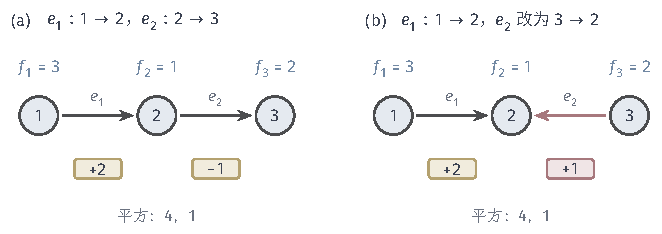
\includegraphics[width=112mm]{figures/01-basic-mathematics/04-graphs/tikz/c6-vertex-edge-functions/figure.pdf}
  \caption{三点路径上的顶点函数与边函数。蓝色数字是顶点值$\bm f=(3,1,2)^{\top}$，方框中是按参考方向计算的边差$(\bm B^{\top}\bm f)_e$（起点减终点）。(a)~$e_1:1\to2$、$e_2:2\to3$，边差为$(2,-1)$；(b)~只把$e_2$改记为$3\to2$（红色），它的边差变为$+1$。单条边差的符号随参考方向改变，平方$4$与$1$不变。}
  \label{fig:graph-spec-vertex-edge-functions}
\end{figure}

单条边差依赖参考方向。把$e_2$改记为$3\to2$，$\bm B$的第二列变号，该边的差从$f_2-f_3=-1$变成$f_3-f_2=1$，而$e_1$的差不受影响，见图~\ref{fig:graph-spec-vertex-edge-functions}。用矩阵表示，一次改记相当于右乘一个对角元为$\pm1$的符号矩阵$\bm R$（改记的边取$-1$），新关联矩阵为$\bm B\bm R$，新边差为$\bm R\bm B^{\top}\bm f$：每个分量至多变号，绝对值与平方都不变。由此得到构造无向图算子的一条要求：结果只能依赖边差的平方或其他不受符号影响的组合，否则它描述的是记账方式，而不是图本身。下一节的拉普拉斯满足这一要求。

% 第6章第2节：图拉普拉斯（邻域汇总、组合拉普拉斯、二次型与沿边变化能量）。

\section{图拉普拉斯}
\label{sec:graph-laplacian}

上一节得到了每条边上的差，但还没有把它们组织成作用于顶点函数的算子。本节沿两条路线构造同一个算子：一条在每个顶点读取邻居并与本点比较，另一条先取边差、再按边权缩放、最后汇总回顶点。两条路线的结果都是组合拉普拉斯，它的二次型累计各边差值的平方，用来衡量函数沿边变化的总量。

\subsection{邻域汇总}
\label{sec:graph-spec-neighborhood-aggregation}

最直接的图上运算是读取邻居。用权矩阵$\bm W$左乘顶点函数，
\[
 (\bm W\bm f)_i=\sum_{j=1}^nw_{i,j}f_j ,
\]
第$i$个输出把各邻居的值按边权加权求和；非邻居的$w_{i,j}=0$，不参与计算。与之相伴的量是顶点$i$的\term{加权度}（weighted degree）
\[
 d_i=\sum_{j=1}^nw_{i,j},\qquad \bm D=\operatorname{diag}(d_1,\ldots,d_n),
\]
它累计与$i$相连的全部边权。第~\ref{sec:graph-adjacency-paths}节的度数的是邻居个数，加权度数的是连接强度，只有每条边权都为$1$时二者才相等。本章后文所说的度一律指加权度。

$\bm W\bm f$是加权和，不是平均。在单位权三点路径上取$\bm f=(3,1,2)^{\top}$，得到$\bm W\bm f=(1,5,1)^{\top}$：中间顶点读到两个邻居之和$5$，比任何一个邻居的值都大。要得到邻居的平均，还须除以加权度，这是第~\ref{sec:graph-normalized-laplacian}节的工作。

\paragraph{同步读取与就地更新}
“作用一次”还有一个容易忽略的约定：所有顶点都从同一份旧向量读取，结果写入另一份新数组。若在原数组上就地按编号逐个更新，后更新的顶点会读到本轮已经改写的值。在上面的例子中按$1,2,3$的次序就地更新：先得$v_1=f_2=1$；更新顶点$2$时读到的是新值$v_1=1$而不是$3$，得$v_2=1+2=3$；再得$v_3=v_2=3$。结果是$(1,3,3)^{\top}$而不是$(1,5,1)^{\top}$。就地更新实现的是另一个与次序有关的映射，不再是$\bm W$。本章所说的算子作用都指同步读取旧值，只涉及一次线性映射，不涉及随时间演化的过程。

\subsection{组合拉普拉斯}
\label{sec:graph-spec-combinatorial-laplacian}

邻域汇总给出了邻居的加权和，衡量变化还需要把本点值与邻居值相比较。对每个邻居取差$f_i-f_j$，再按边权求和，得到
\[
 \sum_{j=1}^nw_{i,j}(f_i-f_j)=d_if_i-(\bm W\bm f)_i .
\]
右端对每个$i$成立，于是这一运算可以写成矩阵$\bm D-\bm W$。

\begin{definition}[组合拉普拉斯]
\label{def:graph-spec-combinatorial-laplacian}
设$\mathcal G=(V,E)$为有限无向图，边权对称非负、无自环，$\bm W$与$\bm D$分别为权矩阵与加权度矩阵。称
\begin{equation}
 \bm L=\bm D-\bm W
 \label{eq:graph-spec-laplacian}
\end{equation}
为$\mathcal G$的\term{组合图拉普拉斯}（combinatorial graph Laplacian），它逐点作用为$(\bm L\bm f)_i=\sum_jw_{i,j}(f_i-f_j)$。
\end{definition}

逐项看，$\bm L$的对角元是加权度$d_i$，非对角元是$-w_{i,j}$；每行之和为$d_i-\sum_jw_{i,j}=0$，所以$\bm L\bm1=\bm0$，常量函数被映成零。这与直觉一致：常量在每条边上都没有差。单位权三点路径的拉普拉斯为
\[
 \bm L=\begin{bmatrix}1&-1&0\\-1&2&-1\\0&-1&1\end{bmatrix},\qquad
 \bm L\begin{bmatrix}3\\1\\2\end{bmatrix}=\begin{bmatrix}2\\-3\\1\end{bmatrix}.
\]
中间顶点的输出$-3$是它与两个邻居之差的和$(1-3)+(1-2)$，负号表示它比邻居低。

\begin{figure}[!htb]
  \centering
  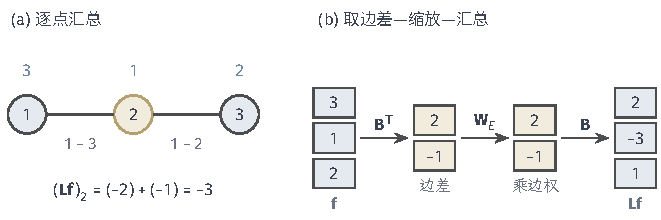
\includegraphics[width=112mm]{figures/01-basic-mathematics/04-graphs/tikz/c6-laplacian-two-routes/figure.pdf}
  \caption{同一个拉普拉斯的两条计算路线，单位权三点路径，$\bm f=(3,1,2)^{\top}$。(a)~在黄色顶点$2$处把本点值与每个邻居值相减再求和，得$(\bm L\bm f)_2=-3$；(b)~先用$\bm B^{\top}$取边差$(2,-1)$，再乘边权（此处均为$1$），最后用$\bm B$按净流出汇总回顶点，得到完整的$\bm L\bm f=(2,-3,1)^{\top}$。两条路线在每个顶点给出相同结果。}
  \label{fig:graph-spec-laplacian-two-routes}
\end{figure}

\paragraph{取边差、缩放、汇总}
第二条路线把上一节的边差接进来：先用$\bm B^{\top}$取边差，再用$\bm W_E$把第$e$条边的差乘以$w_e$，最后用$\bm B$按净流出汇总回顶点。三步合起来是矩阵$\bm B\bm W_E\bm B^{\top}$。为了核对它等于$\bm L$，记$\bm b_e$为$\bm B$的第$e$列，则
\[
 \bm B\bm W_E\bm B^{\top}=\sum_{e\in E}w_e\bm b_e\bm b_e^{\top}.
\]
若$e$连接$i$与$j$，则$\bm b_e=\pm(\bm e_i-\bm e_j)$，$\bm b_e\bm b_e^{\top}$在$(i,i)$、$(j,j)$处为$1$，在$(i,j)$、$(j,i)$处为$-1$，其余为零，而且与参考方向无关。逐边相加，每个对角位置累计出$d_i$，每个非对角位置得到$-w_{i,j}$，因此
\begin{equation}
 \bm L=\bm B\bm W_E\bm B^{\top}.
 \label{eq:graph-spec-laplacian-incidence}
\end{equation}
图~\ref{fig:graph-spec-laplacian-two-routes}在三点路径上并排执行了两条路线。

\paragraph{与参考方向无关}
上一节要求无向图算子不依赖参考方向，式~\eqref{eq:graph-spec-laplacian-incidence}可以整体核对这一点。改记部分边的方向后，关联矩阵变为$\bm B\bm R$，其中$\bm R$是对角元为$\pm1$的符号矩阵。由于对角矩阵相乘可以交换、$\bm R^2=\bm I$，有$\bm R\bm W_E\bm R=\bm W_E$，于是
\[
 (\bm B\bm R)\bm W_E(\bm B\bm R)^{\top}=\bm B\bm R\bm W_E\bm R\bm B^{\top}=\bm B\bm W_E\bm B^{\top}.
\]
边差变号了两次，一次在取差时，一次在汇总时，两次抵消。这一抵消依赖于参考方向只是记账约定；对真正的有向图，弧的方向是数据本身，不能用同样的理由消去，有向图的拉普拉斯一般不对称，不在本章范围内。

\subsection{二次型与沿边变化能量}
\label{sec:graph-spec-dirichlet-energy}

有了算子，再看它的二次型能说明什么。把式~\eqref{eq:graph-spec-laplacian-incidence}代入$\bm f^{\top}\bm L\bm f$，中间恰好是边差的加权平方和：
\begin{equation}
 \begin{aligned}
 \bm f^{\top}\bm L\bm f
 &=(\bm B^{\top}\bm f)^{\top}\bm W_E(\bm B^{\top}\bm f)
 =\sum_{\{i,j\}\in E}w_{i,j}(f_i-f_j)^2\\
 &=\frac12\sum_{i=1}^n\sum_{j=1}^nw_{i,j}(f_i-f_j)^2 .
 \end{aligned}
 \label{eq:graph-spec-dirichlet-energy}
\end{equation}
中间的和对无向边求和，每条边计一次；最右端对有序点对$(i,j)$求和，每条边作为$(i,j)$与$(j,i)$各出现一次，所以要乘$\frac12$。这个量称为沿边变化能量，也称\term{Dirichlet能量}（Dirichlet energy）。它的大小取决于两样东西：相邻值差多少，以及图要求这一对顶点被比较得多强。

\begin{figure}[!htb]
  \centering
  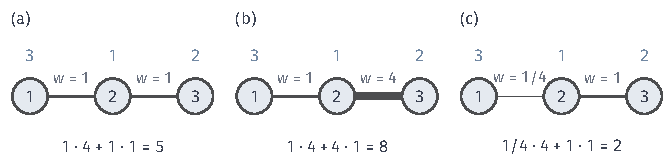
\includegraphics[width=112mm]{figures/01-basic-mathematics/04-graphs/tikz/c6-energy-edge-weights/figure.pdf}
  \caption{同一顶点函数$\bm f=(3,1,2)^{\top}$在三组边权下的沿边变化能量，线宽示意边权大小。两条边的差的平方始终为$4$与$1$，能量是它们的加权和：(a)~权$(1,1)$时为$5$；(b)~加重边$\{2,3\}$后为$8$；(c)~减轻边$\{1,2\}$后为$2$。}
  \label{fig:graph-spec-energy-edge-weights}
\end{figure}

图~\ref{fig:graph-spec-energy-edge-weights}固定$\bm f=(3,1,2)^{\top}$，只改变边权。两条边的差的平方始终是$4$和$1$。单位权时能量为$4+1=5$；把$\{2,3\}$的权加到$4$，较小的差被放大四倍，能量变为$4+4=8$；把$\{1,2\}$的权减到$\frac14$，较大的差几乎不再计入，能量降到$1+1=2$。所以说一个函数“平滑”，总是相对于给定的边权而言的。

\paragraph{半正定与零能量}
式~\eqref{eq:graph-spec-dirichlet-energy}的每一项都是非负权乘平方，所以对任意$\bm f$都有$\bm f^{\top}\bm L\bm f\geq0$。$\bm L$又是对称矩阵，因此它对称半正定（第~\ref{sec:ls-gram-psd}节）。这一结论用到了权非负：若允许负权，对应的项可以为负，半正定性一般不再成立。

能量何时为零？各项非负，总和为零当且仅当每一项为零，即对每条正权边都有$f_i=f_j$；零权边的项本来就是零，不对两端施加任何限制。这是逐边的条件。相等关系怎样沿正权路径传递，零能量的函数究竟有哪些，要用到连通分量，留到第~\ref{sec:graph-spectrum-connectivity}节统一回答。

% 第6章第3节：归一化拉普拉斯（度加权内积、对称归一化拉普拉斯、随机游走拉普拉斯、两种归一化的联系）。

\section{归一化拉普拉斯}
\label{sec:graph-normalized-laplacian}

组合拉普拉斯平等对待每个顶点上的数值。当各顶点的连接总量相差很大时，这种平等会带来偏差：改变连接多的顶点上的值，会同时牵动许多条边。本节先用度给长度加权，再经坐标缩放得到对称归一化拉普拉斯，然后从邻域平均得到随机游走拉普拉斯，最后说明二者的关系。

下面的公式要对加权度取倒数或倒数平方根，只对正度顶点有意义。记$V_+=\{i\in V:d_i>0\}$。度为零的顶点没有任何正权邻边，它在正权支撑图中是孤立点，下文称为支撑孤点；结构上它可能仍连着零权边。每个公式先在正度顶点上建立，再单独约定支撑孤点的处理。

\subsection{度加权内积}
\label{sec:graph-spec-degree-inner-product}

先看连接多少怎样影响能量。图~\ref{fig:graph-spec-degree-weighted-length}是单位权星图，中心连着三片叶，中心的度为$3$，叶的度为$1$。只在中心放一个单位值时，三条边都出现差$1$，能量为$3$；只在一片叶上放同样的单位值，只有一条边有差，能量为$1$。两个函数的欧氏长度都是$1$，能量却相差三倍。原因不在数值本身，而在中心连接更多：同样大小的改动，放在高度顶点上要被更多条边计入。

\begin{figure}[!htb]
  \centering
  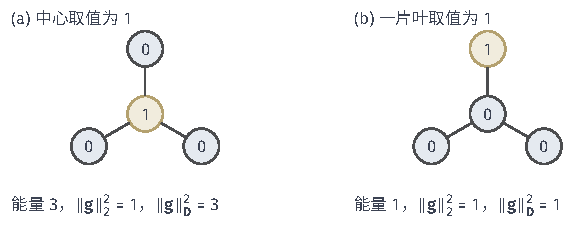
\includegraphics[width=97mm]{figures/01-basic-mathematics/04-graphs/tikz/c6-degree-weighted-length/figure.pdf}
  \caption{单位权星图上的两个单位脉冲，黄色顶点取值$1$，其余为$0$。(a)~中心的度为$3$，能量为$3$；(b)~叶的度为$1$，能量为$1$。两者的欧氏长度平方都是$1$，按度加权的长度平方分别为$3$和$1$，与能量成相同比例。}
  \label{fig:graph-spec-degree-weighted-length}
\end{figure}

如果在衡量函数大小时也把连接量计入，用$\sum_id_ig_i^2$代替$\sum_ig_i^2$，两个脉冲的长度平方就分别是$3$和$1$，能量与长度之比都等于$1$。这提示了一种新的内积：对定义在$V_+$上的函数，令
\begin{equation}
 \langle\bm g,\bm h\rangle_{\bm D}=\bm g^{\top}\bm D\bm h=\sum_{i\in V_+}d_ig_ih_i .
 \label{eq:graph-spec-degree-inner-product}
\end{equation}
在$V_+$上$\bm D$是正对角矩阵，因而对称正定，这正是第~\ref{sec:ls-weighted-inner-products}节的加权内积，称为\term{度加权内积}（degree-weighted inner product）。它与欧氏内积的区别只在于每个顶点的贡献乘以了该点的度。

加权内积可以换回普通内积，办法是缩放坐标。令$\bm f=\bm D^{1/2}\bm g$，即$f_i=\sqrt{d_i}\,g_i$，则
\[
 \lVert\bm f\rVert_2^2=\sum_id_ig_i^2=\bm g^{\top}\bm D\bm g=\lVert\bm g\rVert_{\bm D}^2 .
\]
在新坐标$\bm f$中，度加权长度就是欧氏长度，第三部分关于欧氏内积和对称矩阵的结论可以直接使用。含支撑孤点时，$\bm D$在整个$\mathbb R^n$上是奇异的：取$\bm g$为孤点$v$处的坐标向量$\bm e_v$，有$\bm g^{\top}\bm D\bm g=d_v=0$而$\bm g\neq\bm0$，正定性不成立。所以式~\eqref{eq:graph-spec-degree-inner-product}只在$V_+$上是内积，不能直接称为全空间的内积。

\subsection{对称归一化拉普拉斯}
\label{sec:graph-spec-symmetric-normalized}

先在全体顶点度为正的情形下推导。函数$\bm g$的能量是$\bm g^{\top}\bm L\bm g$，它的度加权长度平方是$\bm g^{\top}\bm D\bm g$。把坐标代换$\bm g=\bm D^{-1/2}\bm f$代入两者，得到
\[
 \frac{\bm g^{\top}\bm L\bm g}{\bm g^{\top}\bm D\bm g}
 =\frac{\bm f^{\top}\bm D^{-1/2}\bm L\bm D^{-1/2}\bm f}{\bm f^{\top}\bm f}.
\]
左端按度衡量的“每单位长度的能量”，在新坐标中变成了一个对称矩阵的普通Rayleigh商（定义~\ref{def:matrix-analysis-rayleigh-quotient}）。这个对称矩阵就是要找的算子。

\begin{definition}[对称归一化拉普拉斯]
\label{def:graph-spec-symmetric-normalized-laplacian}
设全体顶点的加权度为正，称
\begin{equation}
 \bm L_{\mathrm{sym}}=\bm D^{-1/2}\bm L\bm D^{-1/2}=\bm I-\bm D^{-1/2}\bm W\bm D^{-1/2}
 \label{eq:graph-spec-symmetric-normalized-laplacian}
\end{equation}
为\term{对称归一化拉普拉斯}（symmetric normalized Laplacian）。它的对角元为$1$，$(i,j)$位置的非对角元为$-w_{i,j}/\sqrt{d_id_j}$。
\end{definition}

逐边展开它的二次型，可以看出它比较的是什么。$\bm f^{\top}\bm L_{\mathrm{sym}}\bm f$就是$\bm g=\bm D^{-1/2}\bm f$的能量$\bm g^{\top}\bm L\bm g$，把$g_i=f_i/\sqrt{d_i}$代入式~\eqref{eq:graph-spec-dirichlet-energy}，得到
\begin{equation}
 \bm f^{\top}\bm L_{\mathrm{sym}}\bm f=\sum_{\{i,j\}\in E_+}w_{i,j}\left(\frac{f_i}{\sqrt{d_i}}-\frac{f_j}{\sqrt{d_j}}\right)^2\geq0 .
 \label{eq:graph-spec-normalized-energy}
\end{equation}
组合拉普拉斯比较的是相邻顶点的原值，$\bm L_{\mathrm{sym}}$比较的是先除以$\sqrt{d_i}$后的值。求和只经过正权边，而正权边的两个端点度都为正，分母不会出现零。

\paragraph{支撑孤点的约定}
有支撑孤点时，式~\eqref{eq:graph-spec-symmetric-normalized-laplacian}中的$\bm D^{-1/2}$无法按原样定义。约定$\bm D^{-1/2}$是对角矩阵，正度顶点处取$d_i^{-1/2}$，支撑孤点处取$0$，再用$\bm L_{\mathrm{sym}}=\bm D^{-1/2}\bm L\bm D^{-1/2}$定义。支撑孤点$v$在$\bm L$中的行和列本来全为零，在$\bm L_{\mathrm{sym}}$中也全为零，于是对角元$(\bm L_{\mathrm{sym}})_{v,v}=0$。在这一约定下，第二种写法$\bm I-\bm D^{-1/2}\bm W\bm D^{-1/2}$会在孤点处给出$1$，二者不再相同，所以有支撑孤点时只用第一种写法。

以单位权路径$1-2-3$外加孤立顶点$4$为例，度为$(1,2,1,0)$，按约定$\bm D^{-1/2}=\operatorname{diag}(1,\tfrac1{\sqrt2},1,0)$，于是
\[
 \bm L_{\mathrm{sym}}=\begin{bmatrix}1&-\tfrac1{\sqrt2}&0&0\\-\tfrac1{\sqrt2}&1&-\tfrac1{\sqrt2}&0\\0&-\tfrac1{\sqrt2}&1&0\\0&0&0&0\end{bmatrix}.
\]
它的第四行、第四列全为零。二次型~\eqref{eq:graph-spec-normalized-energy}只经过边$\{1,2\}$、$\{2,3\}$，与这个矩阵一致：$f_4$不出现在任何一项中。孤点给$\bm L_{\mathrm{sym}}$带来一个零特征值，它的谱留到第~\ref{sec:graph-spectrum-connectivity}节统一讨论。

\subsection{随机游走拉普拉斯}
\label{sec:graph-spec-random-walk-laplacian}

第~\ref{sec:graph-spec-neighborhood-aggregation}小节指出$\bm W\bm f$是加权和而不是平均。在正度顶点上把第$i$行除以$d_i$，就得到平均：
\[
 \bm P_{\mathrm{rw}}=\bm D^{-1}\bm W,\qquad
 (\bm P_{\mathrm{rw}}\bm f)_i=\sum_j\frac{w_{i,j}}{d_i}f_j .
\]
这里的下标与重编号用的置换矩阵$\bm P$相区别。$\bm P_{\mathrm{rw}}$每行的权非负且和为$1$，所以$(\bm P_{\mathrm{rw}}\bm f)_i$是邻居值的加权平均，介于邻居值的最小值与最大值之间。支撑孤点没有邻居可平均，约定$(\bm P_{\mathrm{rw}})_{v,v}=1$、该行其余元素为$0$，使孤点保持原值。在单位权三点路径上，$\bm P_{\mathrm{rw}}(3,1,2)^{\top}=(1,\tfrac52,1)^{\top}$：中间顶点得到两个邻居的平均$\tfrac52$，不再是和$5$。

本点值减去邻居平均，就得到第三个算子
\begin{equation}
 \bm L_{\mathrm{rw}}=\bm I-\bm P_{\mathrm{rw}} ,
 \label{eq:graph-spec-random-walk-laplacian}
\end{equation}
称为\term{随机游走拉普拉斯}（random-walk Laplacian）。在正度顶点的行上，$\bm L_{\mathrm{rw}}=\bm D^{-1}\bm L$，即$(\bm L_{\mathrm{rw}}\bm f)_i=(\bm L\bm f)_i/d_i$；支撑孤点的行全为零。上例中$\bm L_{\mathrm{rw}}(3,1,2)^{\top}=(2,-\tfrac32,1)^{\top}$，中间顶点的输出是$1-\tfrac52$。

名称中的“随机游走”来自对$w_{i,j}/d_i$的一种解释：把它看成从$i$出发下一步走到$j$的概率。完整的随机游走还需要随机序列和转移规则，它的稳态与收敛属于后续概率部分。本节只使用有限个非负权的加权平均，不涉及任何随机性或收敛结论。

\subsection{两种归一化的联系}
\label{sec:graph-spec-normalization-relations}

$\bm L_{\mathrm{sym}}$由坐标缩放得到，$\bm L_{\mathrm{rw}}$由邻域平均得到，两者其实是同一个作用的两种写法。在正度顶点上，
\[
 \bm D^{-1/2}\bm L_{\mathrm{sym}}\bm D^{1/2}=\bm D^{-1/2}\bm D^{-1/2}\bm L\bm D^{-1/2}\bm D^{1/2}=\bm D^{-1}\bm L=\bm L_{\mathrm{rw}} .
\]
所以二者相似（第~\ref{sec:ls-similarity}节），特征值相同，特征向量要经坐标转换：若$\bm L_{\mathrm{sym}}\bm x=\lambda\bm x$，则$\bm L_{\mathrm{rw}}(\bm D^{-1/2}\bm x)=\lambda\bm D^{-1/2}\bm x$。读法是：$\bm L_{\mathrm{rw}}$作用于原坐标$\bm g$，等于先换到$\bm f=\bm D^{1/2}\bm g$，用$\bm L_{\mathrm{sym}}$作用，再换回原坐标。

$\bm L_{\mathrm{rw}}$一般不对称。单位权三点路径上，它的$(1,2)$元是$-1$，$(2,1)$元是$-\tfrac12$。但它在度加权内积下自伴（第~\ref{sec:ls-adjoints}节）：由$\bm D\bm L_{\mathrm{rw}}=\bm L=\bm L^{\top}$，
\[
 \langle\bm L_{\mathrm{rw}}\bm g,\bm h\rangle_{\bm D}=\bm g^{\top}\bm L_{\mathrm{rw}}^{\top}\bm D\bm h=\bm g^{\top}\bm L\bm h=\langle\bm g,\bm L_{\mathrm{rw}}\bm h\rangle_{\bm D} .
\]
有支撑孤点时，这些关系都限制在正度顶点上成立。

\begin{figure}[!htb]
  \centering
  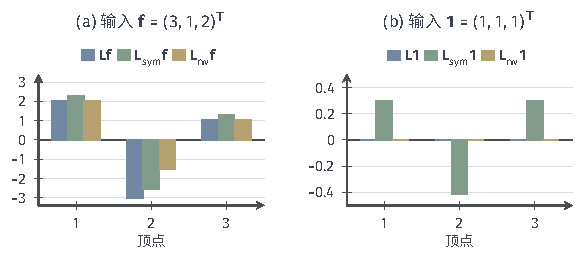
\includegraphics[width=98mm]{figures/01-basic-mathematics/04-graphs/tikz/c6-three-laplacians/figure.pdf}
  \caption{单位权三点路径（度为$1,2,1$）上三种拉普拉斯作用于同一向量。(a)~输入$(3,1,2)^{\top}$：$\bm L_{\mathrm{rw}}$把$\bm L$的输出逐点除以度，中间顶点从$-3$变为$-\tfrac32$；$\bm L_{\mathrm{sym}}$的输出约为$(2.29,-2.54,1.29)$。(b)~输入常量$\bm1$：$\bm L$与$\bm L_{\mathrm{rw}}$都给出零，$\bm L_{\mathrm{sym}}$不给出零。}
  \label{fig:graph-spec-three-laplacians}
\end{figure}

用一个度不相等的例子对照三个算子。单位权三点路径的度为$(1,2,1)$，图~\ref{fig:graph-spec-three-laplacians}(a)把它们作用于$\bm f=(3,1,2)^{\top}$：
\[
 \bm L\bm f=\begin{bmatrix}2\\-3\\1\end{bmatrix},\quad
 \bm L_{\mathrm{rw}}\bm f=\begin{bmatrix}2\\-\tfrac32\\1\end{bmatrix},\quad
 \bm L_{\mathrm{sym}}\bm f=\begin{bmatrix}3-\tfrac1{\sqrt2}\\1-\tfrac5{\sqrt2}\\2-\tfrac1{\sqrt2}\end{bmatrix}\approx\begin{bmatrix}2.29\\-2.54\\1.29\end{bmatrix}.
\]
$\bm L_{\mathrm{rw}}$只是把$\bm L$的输出逐点除以度，度为$1$的端点不变；$\bm L_{\mathrm{sym}}$则先把输入缩放成$\bm D^{-1/2}\bm f=(3,\tfrac1{\sqrt2},2)^{\top}$，再作用、再缩放，每个分量都变了。图~(b)换成常量输入$\bm1$：$\bm L\bm1=\bm L_{\mathrm{rw}}\bm1=\bm0$，而$\bm L_{\mathrm{sym}}\bm1=(1-\tfrac1{\sqrt2},1-\sqrt2,1-\tfrac1{\sqrt2})^{\top}\neq\bm0$。$\bm L_{\mathrm{sym}}$消去的是度缩放后的常量$\bm D^{1/2}\bm1=(1,\sqrt2,1)^{\top}$，因为$\bm L_{\mathrm{sym}}\bm D^{1/2}\bm1=\bm D^{-1/2}\bm L\bm1=\bm0$。

这个例子区分了三件不同的事。从$\bm L$到$\bm L_{\mathrm{rw}}$是改变算子：输出被逐点除以度，零向量不变，但输出的尺度变了。从$\bm L_{\mathrm{rw}}$到$\bm L_{\mathrm{sym}}$是改变坐标：同一个作用在$\bm g$坐标与$\bm f=\bm D^{1/2}\bm g$坐标中分别写成这两个矩阵。把欧氏内积换成度加权内积则是改变内积：$\bm L_{\mathrm{rw}}$在欧氏内积下不对称，在度加权内积下自伴。后面选取谱基、作谱划分时，都要先说明用的是哪个算子、哪种坐标。

% 第6章第4节：图谱与连通性（特征向量与变化尺度、零空间与连通分量、归一化谱界）。

\section{图谱与连通性}
\label{sec:graph-spectrum-connectivity}

前两节建立的$\bm L$与$\bm L_{\mathrm{sym}}$都是实对称矩阵，可以直接使用第三部分的谱定理。本节回答三个问题：特征向量表示怎样的变化模式，零特征值反映了图的什么结构，归一化后的特征值落在什么范围。所选图算子的特征值合起来称为\term{图谱}（graph spectrum）。它由算子和边权决定，不由顶点编号决定，也不是事先给定的物理频率。

\subsection{特征向量与变化尺度}
\label{sec:graph-spec-eigenvectors-scales}

由谱定理（定理~\ref{thm:ls-real-symmetric-spectral}），存在正交矩阵$\bm U=[\bm u_1,\ldots,\bm u_n]$与实对角矩阵$\bm\Lambda$，使
\begin{equation}
 \bm L=\bm U\bm\Lambda\bm U^{\top},\qquad
 \bm\Lambda=\operatorname{diag}(\lambda_1,\ldots,\lambda_n),\qquad
 \lambda_1\leq\lambda_2\leq\cdots\leq\lambda_n .
 \label{eq:graph-spec-laplacian-eigendecomposition}
\end{equation}
按本章约定，特征值从小到大编号。$\bm L$半正定，所以全部$\lambda_k\geq0$；又$\bm L\bm1=\bm0$，所以$\lambda_1=0$。

特征值有一个直接的含义。对单位特征向量$\bm u_k$，
\[
 \bm u_k^{\top}\bm L\bm u_k=\lambda_k\bm u_k^{\top}\bm u_k=\lambda_k ,
\]
即$\lambda_k$就是$\bm u_k$的沿边变化能量。由于长度已经固定为$1$，小特征值对应沿边起伏小的方向，大特征值对应相邻顶点取值差异大的方向。因此常把$\lambda_k$称为\term{图频率}（graph frequency）：把特征值看作频率，特征向量看作该频率的振荡模式，低频平缓、高频剧烈。

\begin{figure}[!htb]
  \centering
  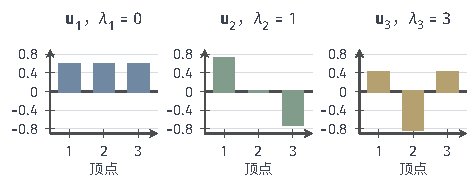
\includegraphics[width=80mm]{figures/01-basic-mathematics/04-graphs/tikz/c6-path-modes/figure.pdf}
  \caption{单位权三点路径的三个标准正交特征向量，条高为各顶点上的取值。$\bm u_1$为常量，能量$0$；$\bm u_2$两端反号、中间为零，变号一次，能量$1$；$\bm u_3$中间与两端反号，变号两次，能量$3$。}
  \label{fig:graph-spec-path-modes}
\end{figure}

单位权三点路径的拉普拉斯可以逐个核对。取
\[
 \bm u_1=\tfrac1{\sqrt3}(1,1,1)^{\top},\qquad
 \bm u_2=\tfrac1{\sqrt2}(1,0,-1)^{\top},\qquad
 \bm u_3=\tfrac1{\sqrt6}(1,-2,1)^{\top}.
\]
直接相乘得$\bm L(1,0,-1)^{\top}=(1,0,-1)^{\top}$、$\bm L(1,-2,1)^{\top}=(3,-6,3)^{\top}$，所以对应特征值为$0,1,3$。用能量逐边核对：$\bm u_2$在两条边上的差都是$\tfrac1{\sqrt2}$，能量$\tfrac12+\tfrac12=1$；$\bm u_3$在两条边上的差都是$\tfrac3{\sqrt6}$，能量$\tfrac96+\tfrac96=3$。图~\ref{fig:graph-spec-path-modes}显示，从常量到左右反向、再到中间与两端反向，变号次数增加，能量随之增大。

图频率依赖边权。把边$\{2,3\}$的权从$1$改为$4$，拉普拉斯变为
\[
 \begin{bmatrix}1&-1&0\\-1&5&-4\\0&-4&4\end{bmatrix},
\]
除零之外的两个特征值满足$\lambda^2-10\lambda+12=0$，即$5\pm\sqrt{13}\approx1.39,\,8.61$。连接关系和顶点次序都没变，谱却变了。所以不能把图频率看成只由无权连接或数组次序决定的固定量。

\paragraph{重编号下的谱}
第~\ref{sec:graph-isomorphism}节用置换矩阵$\bm P$表示顶点重编号，邻接矩阵变为$\bm P\bm A\bm P^{\top}$。度矩阵与权矩阵同步重排，所以拉普拉斯变为$\bm L'=\bm P\bm L\bm P^{\top}$。若$\bm L\bm u=\lambda\bm u$，由$\bm P^{\top}\bm P=\bm I$，
\[
 \bm L'(\bm P\bm u)=\bm P\bm L\bm P^{\top}\bm P\bm u=\bm P\bm L\bm u=\lambda\,\bm P\bm u .
\]
特征值不变，特征向量的分量随顶点一起重排。这区分了三个层次：记录顺序是任意选择的；特征向量在某个记录顺序下的坐标随顺序改变；图谱本身则不依赖记录顺序，是同构图共有的量。

\subsection{零空间与连通分量}
\label{sec:graph-spec-null-space-components}

第~\ref{sec:graph-spec-dirichlet-energy}小节得到了逐边条件：能量为零当且仅当每条正权边两端相等。把这个条件沿路径传递，就能确定全部零特征向量。下面的$\bm1_C$表示顶点集$C$的指示向量，在$C$上取$1$、其余为$0$；连通分量的概念见第~\ref{sec:graph-connectivity-separation}节。

\begin{theorem}[零空间与正权支撑分量]
\label{thm:graph-spec-null-space}
设$\mathcal G$为有限无向图，边权非负对称，正权支撑图$(V,E_+)$的连通分量为$C_1,\ldots,C_c$，则
\[
 \ker\bm L=\operatorname{span}\{\bm1_{C_1},\ldots,\bm1_{C_c}\},
\]
且$\bm L$的零特征值的重数等于$c$。
\end{theorem}

\begin{proof}
第一步，零空间由能量刻画。若$\bm L\bm f=\bm0$，则$\bm f^{\top}\bm L\bm f=\bm f^{\top}\bm0=0$。反过来，把$\bm f=\sum_kc_k\bm u_k$代入，$\bm f^{\top}\bm L\bm f=\sum_k\lambda_kc_k^2$，各项非负，和为零迫使$\lambda_k>0$时$c_k=0$，于是$\bm L\bm f=\sum_k\lambda_kc_k\bm u_k=\bm0$。所以$\bm L\bm f=\bm0$当且仅当$\bm f^{\top}\bm L\bm f=0$，又当且仅当每条正权边两端相等。

第二步，相等关系沿路径传递。若$i$与$j$在同一分量$C$中，则存在一条只经过正权边的路径$i=v_0,v_1,\ldots,v_\ell=j$，逐边得$f_{v_0}=f_{v_1}=\cdots=f_{v_\ell}$。所以零能量的函数在每个分量上取常数。反之，正权边的两个端点总在同一分量中，在各分量上分别取常数的函数，在每条正权边上的差都为零。于是$\ker\bm L$恰为“在每个分量上取常数”的函数全体，每个这样的函数都可写成$\sum_ta_t\bm1_{C_t}$。

第三步，数维数。各分量互不相交，指示向量的支撑互不重叠，两两正交，因而线性无关，$\dim\ker\bm L=c$。在谱分解~\eqref{eq:graph-spec-laplacian-eigendecomposition}中，$\ker\bm L$由$\lambda_k=0$的那些$\bm u_k$张成，所以零特征值恰好出现$c$次。
\end{proof}

这一结论特别给出：$\lambda_2>0$当且仅当正权支撑图连通。图~\ref{fig:graph-spec-component-null-modes}中的图有三个正权支撑分量：路径$\{1,2,3\}$、边$\{4,5\}$和孤点$6$，所以零特征值的重数为$3$（直接计算可得$\bm L$的谱为$0,0,0,1,2,3$）。连接$3$与$4$的零权边结构上存在，但它的能量项恒为零，不迫使两端相等，所以不能把两个分量合并：$\bm1_{C_1}$与$\bm1_{C_2}$可以分别取不同的常数。

\begin{figure}[!htb]
  \centering
  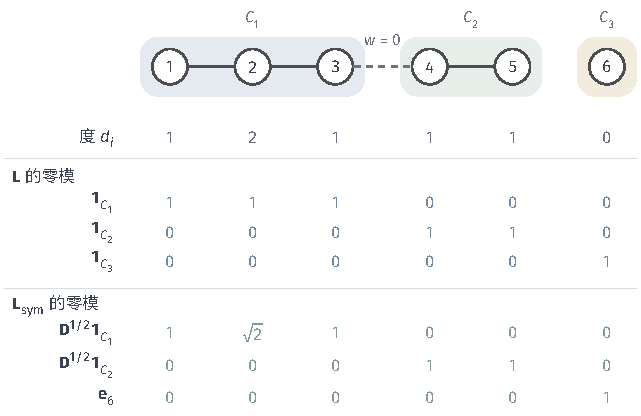
\includegraphics[width=108mm]{figures/01-basic-mathematics/04-graphs/tikz/c6-component-null-modes/figure.pdf}
  \caption{正权支撑分量与零特征向量。实线为单位权边，虚线$\{3,4\}$为零权结构边，顶点$6$为支撑孤点；三块底色标出分量$C_1,C_2,C_3$。上半部分为$\bm L$零空间的一组基，即各分量的指示向量；下半部分为$\bm L_{\mathrm{sym}}$零空间的一组基：正度分量上是度缩放的指示向量$\bm D^{1/2}\bm1_C$，孤点处是坐标方向$\bm e_6$。两组基的个数相同，向量不同。}
  \label{fig:graph-spec-component-null-modes}
\end{figure}

\paragraph{归一化算子的零空间}
同样的论证可以搬到$\bm L_{\mathrm{sym}}$。在正度顶点上，由式~\eqref{eq:graph-spec-normalized-energy}，能量为零当且仅当每条正权边上$f_i/\sqrt{d_i}=f_j/\sqrt{d_j}$，即$\bm D^{-1/2}\bm f$在每个分量上取常数。所以每个含正权边的分量$C$贡献零特征向量$\bm D^{1/2}\bm1_C$。支撑孤点$v$的行与列全为零，坐标方向$\bm e_v$也是零特征向量。合起来，$\bm L_{\mathrm{sym}}$的零特征值重数仍等于正权支撑分量数（孤点自成一个分量），但基向量换成了度缩放的版本。图~\ref{fig:graph-spec-component-null-modes}的下半部分列出了它们，例如$\bm D^{1/2}\bm1_{C_1}=(1,\sqrt2,1,0,0,0)^{\top}$。

普通常量与度缩放常量不能互换。图~\ref{fig:graph-spec-three-laplacians}(b)已经显示$\bm L_{\mathrm{sym}}\bm1\neq\bm0$；只有在一个分量内各点度相同时，二者才成比例。至于$\bm L_{\mathrm{rw}}$，它在正度行上等于$\bm D^{-1}\bm L$，在孤点行上为零，所以$\bm L_{\mathrm{rw}}\bm g=\bm0$当且仅当$\bm L\bm g=\bm0$，零空间仍由普通的分量指示向量张成。

\subsection{归一化谱界}
\label{sec:graph-spec-normalized-bound}

组合拉普拉斯的特征值随边权整体放缩：所有边权乘以$c>0$，$\bm L$乘以$c$，谱也乘以$c$。$\bm L_{\mathrm{sym}}$则不受这种放缩影响，因为$\bm D^{-1/2}$同时乘以$c^{-1/2}$，两侧抵消。下面证明它的特征值总在一个固定区间内。

\begin{theorem}[归一化谱界]
\label{thm:graph-spec-normalized-bound}
对有限无向非负权图，按本节约定定义的$\bm L_{\mathrm{sym}}$满足$0\leq\bm f^{\top}\bm L_{\mathrm{sym}}\bm f\leq2\lVert\bm f\rVert_2^2$，因此它的全部特征值落在$[0,2]$中。
\end{theorem}

\begin{proof}
下界即式~\eqref{eq:graph-spec-normalized-energy}的非负性。对上界，对任意实数$a,b$有$(a-b)^2\leq2(a^2+b^2)$，因为两边之差为$(a+b)^2\geq0$。令$a_i=f_i/\sqrt{d_i}$（$i\in V_+$），逐边使用这一不等式：
\[
 \begin{aligned}
 \sum_{\{i,j\}\in E_+}w_{i,j}(a_i-a_j)^2
 &\leq2\sum_{\{i,j\}\in E_+}w_{i,j}\bigl(a_i^2+a_j^2\bigr)
 =2\sum_{i\in V_+}a_i^2\sum_jw_{i,j}\\
 &=2\sum_{i\in V_+}\frac{f_i^2}{d_i}\,d_i\leq2\lVert\bm f\rVert_2^2 .
 \end{aligned}
\]
中间的等号把每条边上的两项分别归到两个端点，每个顶点$i$收集到的权之和恰为$d_i$；最后一步只是丢掉了支撑孤点上的非负项$f_v^2$。设$\bm x_k$是$\bm L_{\mathrm{sym}}$的单位特征向量，特征值为$\mu_k$，取$\bm f=\bm x_k$即得$0\leq\mu_k=\bm x_k^{\top}\bm L_{\mathrm{sym}}\bm x_k\leq2$；也可以由Rayleigh--Ritz定理（定理~\ref{thm:matrix-analysis-rayleigh-ritz}）读出。
\end{proof}

上界可以取到。单位权三点路径的$\bm L_{\mathrm{sym}}$特征值为$0,1,2$，取到$2$的特征向量是$(1,-\sqrt2,1)^{\top}$，换回原坐标$\bm D^{-1/2}\bm f=(1,-1,1)^{\top}$，相邻顶点正负交替，每条边都达到证明中不等式的等号$a_i=-a_j$。组合拉普拉斯没有同样的统一上界：这条路径的$\bm L$已有特征值$3>2$。同样的论证只给出$\bm f^{\top}\bm L\bm f\leq2\sum_id_if_i^2\leq2d_{\max}\lVert\bm f\rVert_2^2$，上界随最大度和边权的尺度变化。

谱界告诉我们特征值可能出现在哪个区间。第~\ref{sec:graph-filtering}节设计滤波响应、用多项式逼近响应时，只需在这个区间上考虑。谱界本身不是任何迭代算法的收敛保证，那需要另行分析。

% 第6章第5节：图傅里叶变换（谱坐标与重构、环图上的傅里叶基）。

\section{图傅里叶变换}
\label{sec:graph-fourier-transform}
\label{sec:signal-analysis-graph-state-kernels}

上一节的特征向量按变化尺度排成一组标准正交基。本节把顶点函数展开在这组基上：先建立投影系数、重构公式和两种能量的分解，再在规则的环图上说明熟悉的复指数为什么恰好是特征向量。所用的只是有限维正交分解与复数运算，离散傅里叶变换和快速算法留给后续信号部分。

\subsection{谱坐标与重构}
\label{sec:graph-spec-spectral-coordinates}

给定$\bm L$的一组标准正交特征向量$\bm u_1,\ldots,\bm u_n$，按特征值从小到大排成正交矩阵$\bm U$。任意顶点函数都可以在这组基下写出坐标，坐标就是它与各基向量的内积（第~\ref{sec:ls-orthonormal-bases}节）。

\begin{definition}[图傅里叶变换]
\label{def:graph-spec-graph-fourier-transform}
设$\bm L=\bm U\bm\Lambda\bm U^{\top}$为式~\eqref{eq:graph-spec-laplacian-eigendecomposition}的谱分解。顶点函数$\bm f$的\term{图傅里叶变换}（graph Fourier transform）及其逆变换为
\begin{equation}
 \widehat{\bm f}=\bm U^{\top}\bm f,\qquad \bm f=\bm U\widehat{\bm f}=\sum_{k=1}^n\widehat f_k\bm u_k ,
 \label{eq:graph-spec-graph-fourier-transform}
\end{equation}
其中$\widehat f_k=\bm u_k^{\top}\bm f$称为$\bm f$的第$k$个\term{谱坐标}（spectral coordinate）。
\end{definition}

正变换逐个读出$\bm f$在各模态方向上的分量，逆变换再把这些分量乘回对应的基向量相加。因为$\bm U^{\top}\bm U=\bm U\bm U^{\top}=\bm I$，两步互为逆运算，完整换坐标不丢失任何信息。

\begin{figure}[!htb]
  \centering
  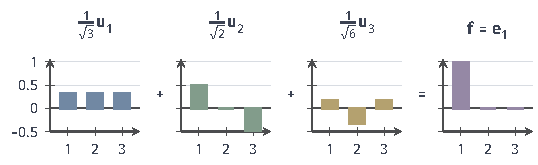
\includegraphics[width=91mm]{figures/01-basic-mathematics/04-graphs/tikz/c6-spectral-projection/figure.pdf}
  \caption{三点路径上单位脉冲的谱展开。前三幅是各模态乘以对应谱坐标后的贡献$\widehat f_k\bm u_k$，分别为$(\tfrac13,\tfrac13,\tfrac13)$、$(\tfrac12,0,-\tfrac12)$与$(\tfrac16,-\tfrac13,\tfrac16)$；逐点相加恰好恢复第四幅的$\bm e_1=(1,0,0)^{\top}$。}
  \label{fig:graph-spec-spectral-projection}
\end{figure}

在单位权三点路径上用第~\ref{sec:graph-spec-eigenvectors-scales}小节的三个模态展开单位脉冲$\bm f=\bm e_1$。三个谱坐标是$\bm u_k$的第一个分量：
\[
 \widehat{\bm f}=\Bigl(\tfrac1{\sqrt3},\tfrac1{\sqrt2},\tfrac1{\sqrt6}\Bigr)^{\top}.
\]
重构时，三个贡献分别是$\tfrac1{\sqrt3}\bm u_1=\tfrac13(1,1,1)^{\top}$、$\tfrac1{\sqrt2}\bm u_2=\tfrac12(1,0,-1)^{\top}$、$\tfrac1{\sqrt6}\bm u_3=\tfrac16(1,-2,1)^{\top}$。第一个分量相加为$\tfrac13+\tfrac12+\tfrac16=1$，第二个为$\tfrac13+0-\tfrac13=0$，第三个为$\tfrac13-\tfrac12+\tfrac16=0$，恰好回到$\bm e_1$，见图~\ref{fig:graph-spec-spectral-projection}。一个集中在一点的函数，需要全部三个模态共同表示。

\paragraph{两种能量的分解}
谱坐标把两种不同的“大小”都拆成逐模态的和。由$\bm U$正交，$\lVert\bm f\rVert_2^2=\lVert\bm U^{\top}\bm f\rVert_2^2$；把$\bm f=\bm U\widehat{\bm f}$代入二次型，交叉项消失（式~\eqref{eq:matrix-analysis-quadratic-spectral-form}）。于是
\begin{equation}
 \lVert\bm f\rVert_2^2=\sum_{k=1}^n\widehat f_k^{\,2},\qquad
 \bm f^{\top}\bm L\bm f=\sum_{k=1}^n\lambda_k\widehat f_k^{\,2}.
 \label{eq:graph-spec-parseval}
\end{equation}
前者是总幅值的平方，各模态平等计入；后者是沿边变化能量，每个模态按自己的特征值加权。对上面的脉冲，$\tfrac13+\tfrac12+\tfrac16=1$，能量为$0\cdot\tfrac13+1\cdot\tfrac12+3\cdot\tfrac16=1$，与直接计算一致：只有边$\{1,2\}$上有差$1$。再取$\bm f=(3,1,2)^{\top}$，谱坐标为$(2\sqrt3,\tfrac1{\sqrt2},\tfrac{\sqrt6}2)^{\top}$，平方和$12+\tfrac12+\tfrac32=14=3^2+1^2+2^2$，能量$0+\tfrac12+3\cdot\tfrac32=5$，与第~\ref{sec:graph-spec-dirichlet-energy}小节的结果相同。这个函数的幅值主要在常量模态上，能量却主要来自高频模态$\bm u_3$。

只保留前$r$个模态，得到$\bm f_r=\sum_{k\leq r}\widehat f_k\bm u_k$。它是$\bm f$在$\operatorname{span}\{\bm u_1,\ldots,\bm u_r\}$上的正交投影（第~\ref{sec:ls-projection-matrices}节），误差平方为$\lVert\bm f-\bm f_r\rVert_2^2=\sum_{k>r}\widehat f_k^{\,2}$。例如$\bm f=(3,1,2)^{\top}$保留前两个模态得$(2,2,2)^{\top}+\tfrac12(1,0,-1)^{\top}=(\tfrac52,2,\tfrac32)^{\top}$，误差平方为$\tfrac32$。截断后丢掉的分量无法恢复，所以这是投影近似，不再是完整的可逆变换。

\paragraph{基的选择自由}
谱坐标依赖所选的基。每个特征向量都可以换成它的相反数，相应的谱坐标随之变号。特征值有重复时自由更大：对应特征空间中的任意一组标准正交基都可以使用，单个谱坐标随基的选取改变。不随基改变的是到每个特征空间的投影，以及同一特征值的谱坐标平方和。所以比较两次计算的谱坐标时，应比较特征子空间上的投影，或者记录所用的基，不能只比较“第$k$个数”。下文的四点环有一对重复特征值，就属于这种情形。

\paragraph{计算代价}
取得谱基本身有代价。对稠密的$n\times n$对称矩阵作完整特征分解，通常需要$O(n^3)$次运算，存储$\bm U$需要$O(n^2)$空间；有了$\bm U$之后，每次正变换或逆变换是一次稠密矩阵乘向量，需要$O(n^2)$次运算。核算时要把两部分分开，不能把预先给定的谱基当作没有成本。大图上常常只求少数几个特征向量，那时得到的是截断投影，不是完整的变换。

\subsection{环图上的傅里叶基}
\label{sec:graph-spec-cycle-fourier-basis}

一般图的特征向量需要数值计算，但规则的环图可以直接写出来。取$N\geq3$个顶点的单位权简单环，顶点按环上次序编号为$r=0,1,\ldots,N-1$，下标按模$N$理解，即顶点$r$与$r\pm1$相邻。每个顶点的度为$2$，拉普拉斯逐点作用为
\[
 (\bm L\bm f)[r]=2f[r]-f[r-1]-f[r+1].
\]
环上每个顶点看到的局部结构都一样，这提示尝试沿环匀速旋转的复指数。对$k=0,1,\ldots,N-1$，令
\begin{equation}
 u_k[r]=\frac1{\sqrt N}\,\mathrm e^{2\pi\mathrm ikr/N}.
 \label{eq:graph-spec-cycle-eigenvector}
\end{equation}
代入并提出公因子$u_k[r]$，再用Euler公式（定理~\ref{thm:ru-euler-formula}）得$\mathrm e^{\mathrm i\theta}+\mathrm e^{-\mathrm i\theta}=2\cos\theta$，于是
\[
 (\bm L\bm u_k)[r]=u_k[r]\bigl(2-\mathrm e^{-2\pi\mathrm ik/N}-\mathrm e^{2\pi\mathrm ik/N}\bigr)
 =\Bigl(2-2\cos\frac{2\pi k}N\Bigr)u_k[r].
\]
所以$\bm u_k$是特征向量，特征值为$\lambda_k=2-2\cos(2\pi k/N)$。环的循环下标保证了$r=0$与$r=N-1$处的计算与其他位置相同，因为$\mathrm e^{2\pi\mathrm ikN/N}=1$。

这些向量是复向量，正交性要用复内积$\langle\bm x,\bm y\rangle=\bm x^*\bm y$来检验，其中$^*$表示共轭转置（第~\ref{sec:ls-inner-product-definition}节）。对$0\leq k,l\leq N-1$，
\[
 \langle\bm u_k,\bm u_l\rangle=\frac1N\sum_{r=0}^{N-1}\mathrm e^{2\pi\mathrm i(l-k)r/N}.
\]
$l=k$时每项为$1$，和为$1$。$l\neq k$时令$\rho=\mathrm e^{2\pi\mathrm i(l-k)/N}$，由$0<|l-k|<N$知$\rho\neq1$，而$\rho^N=1$；有限几何和公式（式~\eqref{eq:prelim-finite-geometric-sum}）的推导只用到乘法与减法，对复数公比同样成立，于是和为$(1-\rho^N)/(1-\rho)=0$。所以$\bm u_0,\ldots,\bm u_{N-1}$是$\mathbb C^N$的标准正交基，排成的矩阵$\bm U$满足$\bm U^*\bm U=\bm I$，是酉矩阵（第~\ref{sec:ls-adjoints}节）。相应地，正变换必须使用共轭转置：
\[
 \widehat{\bm f}=\bm U^*\bm f,\qquad \bm f=\bm U\widehat{\bm f},\qquad \lVert\bm f\rVert_2^2=\sum_k|\widehat f_k|^2 .
\]
$\bm L$是实对称矩阵，也有实的特征向量，例如$\bm u_k$与$\bm u_{N-k}$的实部和虚部；用复指数只是因为它对所有$k$给出统一的公式。

\begin{figure}[!htb]
  \centering
  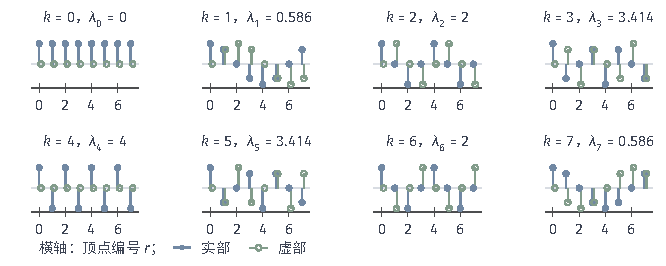
\includegraphics[width=112mm]{figures/01-basic-mathematics/04-graphs/tikz/c6-cycle-fourier-basis/figure.pdf}
  \caption{八点单位权环的复指数特征向量$u_k[r]=\mathrm e^{2\pi\mathrm ikr/8}/\sqrt8$。蓝色实心为实部，绿色空心为虚部，横轴为顶点编号$r$，标题给出特征值$\lambda_k=2-2\cos(2\pi k/8)$。$k$与$8-k$的实部相同、虚部相反，特征值相等；按$k$排列时特征值先增后减，$k=4$的振荡最快。}
  \label{fig:graph-spec-cycle-fourier-basis}
\end{figure}

图~\ref{fig:graph-spec-cycle-fourier-basis}画出$N=8$时的全部八个特征向量。编号$k$是复振荡沿环转动的圈数，不是特征值的次序：特征值随$k$先增后减，$k$与$N-k$给出相同的特征值。原因是$\bm u_{N-k}=\overline{\bm u_k}$，二者沿相反方向转动，相邻顶点间的差异一样大。

\paragraph{四点环上的单位脉冲}
取$N=4$，此时$u_k[r]=\tfrac12\mathrm i^{kr}$，特征值依次为$\lambda_0=0$、$\lambda_1=2$、$\lambda_2=4$、$\lambda_3=2$，其中$\lambda_1=\lambda_3$是一对重复特征值。对顶点$0$上的单位脉冲$\bm f=\bm e_0$，
\[
 \widehat f_k=\sum_r\overline{u_k[r]}f[r]=\overline{u_k[0]}=\tfrac12,\qquad k=0,1,2,3 ,
\]
四个谱坐标都是$\tfrac12$。重构时，$f[r]=\sum_k\tfrac12\cdot\tfrac12\mathrm i^{kr}=\tfrac14\sum_{k=0}^3\mathrm i^{kr}$：$r=0$时为$1$；$r=1,2,3$时公比$\mathrm i^r\neq1$且$(\mathrm i^r)^4=1$，几何和为零。于是恢复了$\bm e_0$。若把脉冲移到顶点$1$，谱坐标变为$\overline{u_k[1]}=\tfrac12\mathrm i^{-k}$，即$\tfrac12,-\tfrac{\mathrm i}2,-\tfrac12,\tfrac{\mathrm i}2$：模都不变，只是辐角随$k$转动。沿环平移只改变各谱坐标的相位，这正是复指数基在环上的方便之处。

这组复指数与信号处理中离散傅里叶变换使用的振荡是同一组，只差归一化常数$\sqrt N$。完整的离散傅里叶变换及其快速算法由后续信号部分展开。环的特殊之处在于存在把每个顶点移到下一个顶点的平移，复指数正是在平移下只改变相位的函数；一般图没有这样的平移，按顶点编号对数组做快速傅里叶变换，得不到该图拉普拉斯的谱坐标。

% 第6章第6节：图滤波（滤波问题与谱响应、基于谱分解的滤波、多项式滤波与局部计算、方法比较与结果检验）。

\section{图滤波}
\label{sec:graph-filtering}

图傅里叶变换只换坐标，不改变函数。本节转向改变函数：规定每个模态保留多少、衰减多少，得到新的顶点函数。先定义滤波的目标，再比较两种实现：一种先求谱基再逐模态缩放，另一种只用拉普拉斯的稀疏乘法。若目标响应在图谱上恰好可以由所用多项式表示，两种实现给出同一个输出；若只是用多项式近似，就需要控制输出误差。

\subsection{滤波问题与谱响应}
\label{sec:graph-spec-filtering-problem}

传感器读数常混有逐点跳动的噪声，而真实的温度场在相邻测点间变化平缓。上一节的分解~\eqref{eq:graph-spec-parseval}说明，逐点跳动主要落在大特征值的模态上。于是“去噪”可以表述为：保留小特征值的模态，压低大特征值的模态。把每个模态保留的比例写成特征值的函数，就得到下面的定义。

\begin{definition}[谱滤波]
\label{def:graph-spec-spectral-filter}
给定图算子$\bm L=\bm U\bm\Lambda\bm U^{\top}$、输入$\bm f$和定义在全部特征值上的实函数$g$，称
\begin{equation}
 \bm y=g(\bm L)\bm f=\bm U\,g(\bm\Lambda)\,\bm U^{\top}\bm f,\qquad
 g(\bm\Lambda)=\operatorname{diag}\bigl(g(\lambda_1),\ldots,g(\lambda_n)\bigr)
 \label{eq:graph-spec-spectral-filter}
\end{equation}
为$\bm f$经\term{谱响应}（spectral response）$g$的\term{图滤波}（graph filtering）输出。按谱坐标写，$\widehat y_k=g(\lambda_k)\widehat f_k$。
\end{definition}

$g(\bm L)$正是第~\ref{sec:ls-matrix-functions}节沿特征方向定义的矩阵函数。几种典型响应各有含义：$g\equiv1$时$\bm y=\bm f$，原样输出；$g(0)=1$保证零模不变，在正权支撑连通时就是保持各点的平均值；$g$随$\lambda$递减到接近零，则高频模态被压低，输出比输入平缓，这样的响应称为低通。这里规定的是要得到什么输出，下面两小节讨论怎样算出它。

\paragraph{定义的合理性}
$\bm U$不唯一，需要确认输出不依赖它的选取。式~\eqref{eq:graph-spec-spectral-filter}对同一特征值的各个模态使用同一个数$g(\lambda)$，所以$g(\bm L)=\sum_\lambda g(\lambda)\bm P_\lambda$，其中$\bm P_\lambda$是到特征空间的正交投影，只由$\bm L$决定（第~\ref{sec:ls-matrix-functions}节）。重编号也不改变结果：$\bm P\bm L\bm P^{\top}$的特征向量是$\bm P\bm u_k$，特征值不变，于是$g(\bm P\bm L\bm P^{\top})=\bm Pg(\bm L)\bm P^{\top}$，对重排后的输入$\bm P\bm f$输出$\bm P\bm y$，即输出随顶点一起重排。

\paragraph{放大界}
滤波可能把函数放大，放大多少由响应的最大幅度控制。由式~\eqref{eq:graph-spec-parseval}，
\begin{equation}
 \begin{gathered}
 \lVert\bm y\rVert_2^2=\sum_kg(\lambda_k)^2\widehat f_k^{\,2}\leq\Bigl(\max_k|g(\lambda_k)|\Bigr)^2\lVert\bm f\rVert_2^2,\\
 \bm y^{\top}\bm L\bm y=\sum_k\lambda_kg(\lambda_k)^2\widehat f_k^{\,2}\leq\Bigl(\max_k|g(\lambda_k)|\Bigr)^2\bm f^{\top}\bm L\bm f .
 \end{gathered}
 \label{eq:graph-spec-filter-bound}
\end{equation}
所以只要在全部特征值上$|g(\lambda_k)|\leq1$，输出的幅值和沿边变化能量都不会超过输入。没有这个条件，就不能断言滤波不增加幅值或能量；例如$g(\lambda)=1+\lambda$会放大高频模态。

\subsection{基于谱分解的滤波}
\label{sec:graph-spec-eigendecomposition-filter}

最直接的实现照搬定义：先求谱基，再在谱坐标中逐个缩放。

\begin{algorithm}[基于谱分解的图滤波]
\label{alg:graph-spec-eigendecomposition-filter}
输入：$n\times n$实对称图算子$\bm L$，顶点函数$\bm f$，谱响应$g$。输出：$\bm y=g(\bm L)\bm f$。
\begin{enumerate}
 \item 求谱分解$\bm L=\bm U\bm\Lambda\bm U^{\top}$（同一个$\bm L$只需做一次）。
 \item 投影：$\widehat{\bm f}=\bm U^{\top}\bm f$。
 \item 逐模态缩放：$\widehat y_k=g(\lambda_k)\widehat f_k$，$k=1,\ldots,n$。
 \item 重构：$\bm y=\bm U\widehat{\bm y}$。
\end{enumerate}
\end{algorithm}

三步合起来是$\bm U g(\bm\Lambda)\bm U^{\top}\bm f$，正确性直接来自定义。开销要分开计：第1步对稠密矩阵通常需要$O(n^3)$次运算，存储$\bm U$需要$O(n^2)$空间；第2、4步各是一次稠密矩阵乘向量，第3步计算$n$个响应值，合计每个输入$O(n^2)$。图算子固定、要处理许多个输入时，第1步的结果可以反复使用，摊到每个输入上的代价随之下降。若为节省开销只求前若干个模态、把其余模态的响应当作零，就改变了目标响应，实际计算的是另一种截断滤波，需要另行说明误差，不能仍称为原响应的精确实现。

\paragraph{三点路径上的低通滤波}
在单位权三点路径上取$\bm f=(3,1,2)^{\top}$与响应$g(\lambda)=1/(1+\lambda)$。上一节已求出谱坐标$\widehat{\bm f}=(2\sqrt3,\tfrac1{\sqrt2},\tfrac{\sqrt6}2)^{\top}$，三个特征值$0,1,3$的响应为$1,\tfrac12,\tfrac14$，所以
\[
 \bm y=2\sqrt3\,\bm u_1+\tfrac12\cdot\tfrac1{\sqrt2}\,\bm u_2+\tfrac14\cdot\tfrac{\sqrt6}2\,\bm u_3
 =\begin{bmatrix}2\\2\\2\end{bmatrix}+\frac14\begin{bmatrix}1\\0\\-1\end{bmatrix}+\frac18\begin{bmatrix}1\\-2\\1\end{bmatrix}
 =\begin{bmatrix}19/8\\7/4\\15/8\end{bmatrix}.
\]
常量成分$(2,2,2)^{\top}$原样保留，所以输出各分量之和仍为$6$；两个变化成分分别缩小为原来的$\tfrac12$和$\tfrac14$。输出的能量为$(\tfrac58)^2+(\tfrac18)^2=\tfrac{13}{32}\approx0.41$，远小于输入的$5$。这个响应恰好对应求解线性方程组：$g(\bm L)=(\bm I+\bm L)^{-1}$，可以直接核对$(\bm I+\bm L)\bm y=\bm f$。

\subsection{多项式滤波与局部计算}
\label{sec:graph-spec-polynomial-filter}

谱分解的代价主要花在求$\bm U$上。若响应是多项式，可以完全绕开特征向量。设$g(\lambda)=\sum_{r=0}^K\alpha_r\lambda^r$，由$\bm L^r=\bm U\bm\Lambda^r\bm U^{\top}$，
\begin{equation}
 g(\bm L)\bm f=\sum_{r=0}^K\alpha_r\bm L^r\bm f ,
 \label{eq:graph-spec-polynomial-filter}
\end{equation}
右端只需要反复用$\bm L$乘向量。按这种方式计算谱滤波称为\term{多项式图滤波}（polynomial graph filtering）。

\begin{algorithm}[多项式图滤波]
\label{alg:graph-spec-polynomial-filter}
输入：以正权边邻接表存储的$\bm L$，顶点函数$\bm f$，系数$\alpha_0,\ldots,\alpha_K$。输出：$\bm y=\sum_r\alpha_r\bm L^r\bm f$。状态：当前幂次向量$\bm v^{(r)}=\bm L^r\bm f$与累加向量$\bm y$。
\begin{enumerate}
 \item 置$\bm v^{(0)}=\bm f$，$\bm y=\alpha_0\bm f$。
 \item 对$r=1,\ldots,K$：从完整的旧向量$\bm v^{(r-1)}$读取，按$(\bm L\bm v)_i=d_iv_i-\sum_jw_{i,j}v_j$把结果写入另一个缓冲区，得到$\bm v^{(r)}$；再令$\bm y\leftarrow\bm y+\alpha_r\bm v^{(r)}$。
\end{enumerate}
\end{algorithm}

第2步必须同步读取旧向量，理由与第~\ref{sec:graph-spec-neighborhood-aggregation}小节相同：就地改写会让后面的顶点读到本轮的新值，算出的就不再是$\bm L\bm v$。按归纳，每轮结束时$\bm v^{(r)}=\bm L^r\bm f$，$\bm y$累加了前$r$项，所以算法输出式~\eqref{eq:graph-spec-polynomial-filter}。

\paragraph{依赖范围}
多项式滤波的输出只依赖附近的顶点。一次乘法中，$(\bm L\bm v)_i$只读取$v_i$与正权邻居的值。归纳可得，$(\bm L^r\bm v)_i$只依赖在正权支撑图中与$i$相距至多$r$步的顶点：第$r$轮读取的邻居值本身只依赖再远$r-1$步以内的顶点。所以$K$次多项式滤波在顶点$i$的输出，只依赖$i$的$K$跳邻域。

这是范围的上界，不是说范围内的每个顶点都一定产生非零贡献。单位权三点路径上，$(\bm L^2-3\bm L)\bm e_1=(2,-3,1)^{\top}-3(1,-1,0)^{\top}=(-1,0,1)^{\top}$：顶点$2$与顶点$1$只隔一条边，但两项贡献恰好相消，输出为零。

\begin{figure}[!htb]
  \centering
  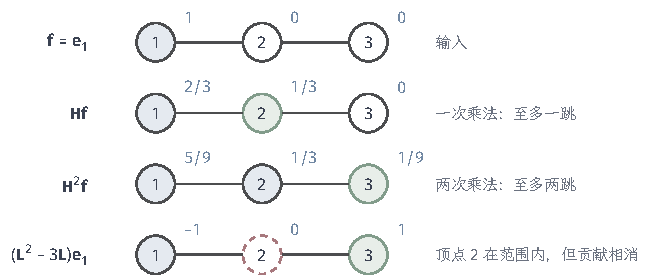
\includegraphics[width=110mm]{figures/01-basic-mathematics/04-graphs/tikz/c6-polynomial-locality/figure.pdf}
  \caption{单位权三点路径上多项式滤波的依赖范围，$\bm H=\bm I-\bm L/3$，蓝色数字为各顶点的输出。从$\bm f=\bm e_1$出发，一次作用只到达一跳邻居（绿色），两次作用才到达两跳外的顶点$3$。最后一行$(\bm L^2-3\bm L)\bm e_1$中，顶点$2$位于范围内，但贡献相消为零（红色虚线）。}
  \label{fig:graph-spec-polynomial-locality}
\end{figure}

图~\ref{fig:graph-spec-polynomial-locality}用一次多项式$\bm H=\bm I-\bm L/3$展示范围怎样扩大。从$\bm e_1$出发，
\[
 \bm H\bm e_1=\bm e_1-\tfrac13(1,-1,0)^{\top}=\bigl(\tfrac23,\tfrac13,0\bigr)^{\top},\qquad
 \bm H^2\bm e_1=\bigl(\tfrac59,\tfrac13,\tfrac19\bigr)^{\top}.
\]
第一轮只有顶点$1$、$2$非零，第二轮才到达顶点$3$。从谱的角度看，$\bm H$的响应$1-\lambda/3$在特征值$0,1,3$上取$1,\tfrac23,0$：常量模态保留，最高频模态被完全消去。

\paragraph{开销与近似误差}
以邻接表存储正权边，一次$\bm L$乘向量要访问每个顶点和每条正权边常数次，需要$O(n+m_+)$次运算；$K$轮共$O(K(n+m_+))$。除了图本身，只需保存旧向量、新向量和累加向量，额外空间为$O(n)$。整个过程不求任何特征向量。

多项式能表示的响应有限，一般的响应$g$只能近似。设多项式$p$在一个包含全部特征值的区间上满足$|g(\lambda)-p(\lambda)|\leq\varepsilon$。对差$g-p$使用放大界~\eqref{eq:graph-spec-filter-bound}，得
\[
 \lVert g(\bm L)\bm f-p(\bm L)\bm f\rVert_2\leq\varepsilon\lVert\bm f\rVert_2 .
\]
所以只要知道谱落在哪个区间，就能把标量函数的逼近误差转成输出误差。对$\bm L_{\mathrm{sym}}$，定理~\ref{thm:graph-spec-normalized-bound}给出区间$[0,2]$；对$\bm L$可用$[0,2d_{\max}]$。图~\ref{fig:graph-spec-filter-responses}(b)在$[0,2]$上逼近低通响应$1/(1+3\lambda)$：用Chebyshev节点插值，$K=2$时最大误差约$0.18$，$K=4$时约$0.038$。

\begin{figure}[!htb]
  \centering
  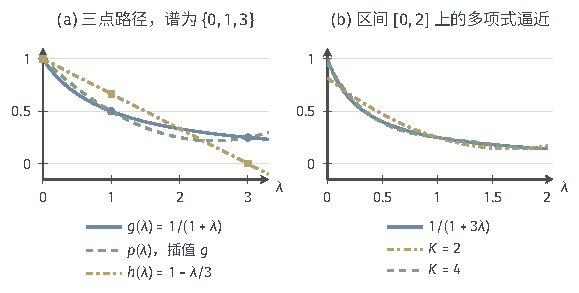
\includegraphics[width=98mm]{figures/01-basic-mathematics/04-graphs/tikz/c6-filter-responses/figure.pdf}
  \caption{谱响应与多项式。(a)~三点路径的谱为$\{0,1,3\}$：蓝色为目标$g(\lambda)=1/(1+\lambda)$，绿色虚线为在三个特征值上与$g$相等的二次多项式$p(\lambda)=1-\tfrac58\lambda+\tfrac18\lambda^2$，二者只在圆点处重合；黄色点划线为$h(\lambda)=1-\lambda/3$，方点是它在特征值上的取值。(b)~区间$[0,2]$上目标$1/(1+3\lambda)$及其$K=2$、$K=4$次Chebyshev节点插值，最大误差约为$0.18$和$0.038$。}
  \label{fig:graph-spec-filter-responses}
\end{figure}

另一种情形是已知全部互不相同的特征值。一个有限集合上的任意函数都可以用插值多项式精确匹配，$s$个不同的特征值需要至多$s-1$次。三点路径的谱为$\{0,1,3\}$，取$p(\lambda)=1-\tfrac58\lambda+\tfrac18\lambda^2$，直接代入得$p(0)=1$、$p(1)=\tfrac12$、$p(3)=\tfrac14$，与$g(\lambda)=1/(1+\lambda)$在三个特征值上相同。于是$p(\bm L)=g(\bm L)$，尽管$p$与$g$作为函数并不相同，见图~\ref{fig:graph-spec-filter-responses}(a)。这种精确匹配要求事先知道特征值，在大图上通常做不到。

\subsection{方法比较与结果检验}
\label{sec:graph-spec-filter-comparison}

比较两种实现时，要固定同一个图算子、同一个输入和同一个目标响应，只比较计算方式。表~\ref{tab:graph-spec-filter-comparison}列出主要差别。

\begin{table}[!htb]
  \centering\small
  \begin{tabularx}{\linewidth}{@{}lXX@{}}
    \toprule
    & 基于谱分解（算法~\ref{alg:graph-spec-eigendecomposition-filter}） & 多项式滤波（算法~\ref{alg:graph-spec-polynomial-filter}）\\
    \midrule
    预处理 & 稠密特征分解，$O(n^3)$ & 无；逼近一般响应时需要谱区间 \\
    单个输入 & $O(n^2)$ & $O(K(n+m_+))$ \\
    额外存储 & $\bm U$，$O(n^2)$ & 三个向量，$O(n)$ \\
    适用响应 & 任意$g$，精确 & 多项式精确；一般$g$有误差$\varepsilon\lVert\bm f\rVert_2$ \\
    \bottomrule
  \end{tabularx}
  \caption{同一图算子、输入和目标响应下两种滤波实现的比较。$n$为顶点数，$m_+$为正权边数，$K$为多项式次数。}
  \label{tab:graph-spec-filter-comparison}
\end{table}

多项式响应可以用两种方法实现同一个算子，结果相同；用多项式逼近一般响应，则在实现方式之外又改变了目标，多出一项近似误差。这两种差别要分开说明，不能把“实现方式不同”和“目标响应不同”混为一谈。

\paragraph{交叉核对}
在小图上，可以用两种实现互相核对。仍取三点路径、$\bm f=(3,1,2)^{\top}$，用插值多项式$p$按算法~\ref{alg:graph-spec-polynomial-filter}计算：$\bm L\bm f=(2,-3,1)^{\top}$，$\bm L^2\bm f=(5,-9,4)^{\top}$，
\[
 p(\bm L)\bm f=\bm f-\tfrac58\bm L\bm f+\tfrac18\bm L^2\bm f
 =\Bigl(3-\tfrac{10}8+\tfrac58,\ 1+\tfrac{15}8-\tfrac98,\ 2-\tfrac58+\tfrac48\Bigr)^{\top}
 =\Bigl(\tfrac{19}8,\tfrac74,\tfrac{15}8\Bigr)^{\top},
\]
与谱分解的结果完全一致，而这次计算没有用到任何特征向量。还可以检查几项必然成立的性质：$\max_k|g(\lambda_k)|=1$，按放大界应有$\lVert\bm y\rVert_2^2\leq\lVert\bm f\rVert_2^2$，实际为$\tfrac{782}{64}\approx12.2\leq14$；$g(0)=1$且图连通，各分量之和应保持为$6$；把顶点重编号后重算，输出应随之重排。

本节的滤波只依赖有限维谱分解，没有引入时间。连续的热扩散及其时间离散会给出特定的响应族，它们在后续过程与信号部分建立。

% 第6章第7节：谱划分（图划分问题与割的表示、RatioCut谱方法、NCut谱方法）。

\section{谱划分}
\label{sec:graph-spectral-partition}

最后回到章首的第三个问题：按连接强弱把顶点分成两组。本节固定$n\geq2$，要求两组都非空。先用指示向量把跨组边权写成拉普拉斯的二次型，说明只最小化跨组边权为什么会得到失衡的划分；再分别按顶点数和连接体积引入平衡，把离散问题写成Rayleigh商，放宽取值限制后用谱展开求解。连续解给出下界和候选分组，但它本身不是分组，二者要始终分开。

\subsection{图划分问题与割的表示}
\label{sec:graph-spec-partition-problem}

把顶点集分成$S$与$\bar S=V\setminus S$两组，跨组的连接强度用
\[
 \operatorname{cut}(S,\bar S)=\sum_{i\in S}\sum_{j\in\bar S}w_{i,j}
\]
衡量。这沿用了第~\ref{sec:graph-max-flow}节割的想法：把顶点分到两侧，累计跨过两侧的边上的数值。区别在于这里的图是无向的，没有源和汇，两个方向不加区分。

割权可以写成二次型。令$\bm s$为$S$的指示向量，$s_i=1$（$i\in S$）或$0$（$i\in\bar S$）。代入能量式~\eqref{eq:graph-spec-dirichlet-energy}，两端在同一组的边$(s_i-s_j)^2=0$，跨组的边$(s_i-s_j)^2=1$，所以
\begin{equation}
 \bm s^{\top}\bm L\bm s=\sum_{\{i,j\}\in E}w_{i,j}(s_i-s_j)^2=\operatorname{cut}(S,\bar S).
 \label{eq:graph-spec-cut-quadratic}
\end{equation}
于是划分问题变成在取值为$0$或$1$的向量上最小化$\bm L$的二次型。

只最小化割权并不够。若允许空组，$S=\varnothing$的割权为零，问题平凡；这正是要求两组非空的原因。即使要求非空，最小割也常常只切下一个连接很弱的顶点。图~\ref{fig:graph-spec-cut-indicator}中两个单位权三角形由一条单位权边相连，顶点$7$以权$0.6$挂在顶点$2$上。直观的分法是沿中间的桥切开，割权为$1$；但只切下顶点$7$的割权是$0.6$，枚举全部$63$种非空二分可知它就是最小割。单纯的割权不关心两组各有多大。

\begin{figure}[!htb]
  \centering
  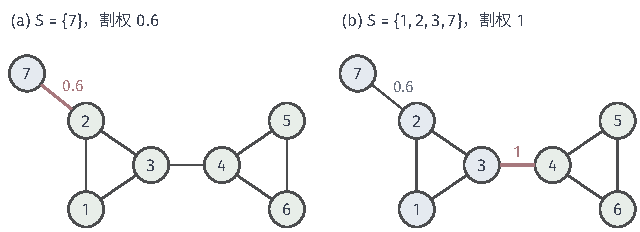
\includegraphics[width=108mm]{figures/01-basic-mathematics/04-graphs/tikz/c6-cut-indicator/figure.pdf}
  \caption{割与指示向量。两个单位权三角形由桥$\{3,4\}$相连，顶点$7$以权$0.6$连到顶点$2$。蓝色顶点属于$S$（指示向量取$1$），绿色顶点属于$\bar S$（取$0$），红色边跨组，$\bm s^{\top}\bm L\bm s$等于红色边权之和。(a)~$S=\{7\}$，割权$0.6$，是全部非空二分中的最小割；(b)~$S=\{1,2,3,7\}$，割权$1$，两组大小相近。}
  \label{fig:graph-spec-cut-indicator}
\end{figure}

\paragraph{松弛给出的上下界}
下面两小节都采用同一种论证，这里先把逻辑说清。设离散问题在有限可行集$\mathcal F$上最小化目标$J$，最优值为$J^\star$。若把可行集扩大为$\mathcal C\supseteq\mathcal F$，并把$J$延拓到$\mathcal C$上，可选的对象只多不少，最小值只能下降：$L=\min_{\mathcal C}J\leq J^\star$。这种做法称为\term{连续松弛}（continuous relaxation），它给出下界。另一方面，从连续解出发构造任意一个合法分组并计算原目标值$U$，则$U\geq J^\star$，它给出上界。于是
\[
 0\leq U-J^\star\leq U-L ,
\]
差$U-L$限制了所得分组可能的次优程度。它只是次优程度的上界，只有下界恰好取到$J^\star$时才等于真实的差距。

\subsection{RatioCut谱方法}
\label{sec:graph-spec-ratio-cut}

为了不让一组过小，把割权按两组的顶点数放大。设$a=|S|>0$，$b=|\bar S|>0$，定义\term{比率割}（RatioCut）
\begin{equation}
 \operatorname{RatioCut}(S,\bar S)=\operatorname{cut}(S,\bar S)\Bigl(\frac1a+\frac1b\Bigr).
 \label{eq:graph-spec-ratio-cut}
\end{equation}
一组越小，$\frac1a$越大，切下它的代价就越高。在图~\ref{fig:graph-spec-cut-indicator}中，只切下顶点$7$的RatioCut为$0.6\cdot(1+\tfrac16)=0.7$，沿桥切开的RatioCut为$1\cdot(\tfrac14+\tfrac13)=\tfrac7{12}\approx0.58$；枚举可知后者是全部非空二分中的最小值。

\paragraph{两水平向量}
接下来把RatioCut写成Rayleigh商。对给定分组构造在两组上分别取常数的向量
\begin{equation}
 f_i=\sqrt{b/a}\quad(i\in S),\qquad f_i=-\sqrt{a/b}\quad(i\in\bar S).
 \label{eq:graph-spec-ratio-cut-vector}
\end{equation}
逐项计算：$\bm1^{\top}\bm f=a\sqrt{b/a}-b\sqrt{a/b}=\sqrt{ab}-\sqrt{ab}=0$；$\bm f^{\top}\bm f=a\cdot\tfrac ba+b\cdot\tfrac ab=n$；跨组边上的差都是$\sqrt{b/a}+\sqrt{a/b}=n/\sqrt{ab}$，同组边上的差为零，所以
\[
 \bm f^{\top}\bm L\bm f=\operatorname{cut}(S,\bar S)\frac{n^2}{ab}=n\operatorname{cut}(S,\bar S)\Bigl(\frac1a+\frac1b\Bigr)=n\operatorname{RatioCut}(S,\bar S).
\]
因此$\operatorname{RatioCut}(S,\bar S)=\bm f^{\top}\bm L\bm f/\bm f^{\top}\bm f$。最小化RatioCut，等价于在“与$\bm1$正交、只取两个由分组决定的值”的向量中最小化$\bm L$的Rayleigh商。去掉“只取两个值”的限制，只保留$\bm f\neq\bm0$与$\bm f\perp\bm1$，可行集从有限个向量扩大为一个$n-1$维子空间去掉原点，这就是连续松弛。

\begin{theorem}[RatioCut的谱下界]
\label{thm:graph-spec-ratio-cut-bound}
设$\bm L$的特征值为$0=\lambda_1\leq\lambda_2\leq\cdots\leq\lambda_n$，则
\[
 \min_{\bm f\neq\bm0,\ \bm f\perp\bm1}\frac{\bm f^{\top}\bm L\bm f}{\bm f^{\top}\bm f}=\lambda_2 ,
\]
最小值在第二特征向量$\bm u_2$处取到。因此对每个非空二分都有$\operatorname{RatioCut}(S,\bar S)\geq\lambda_2$。
\end{theorem}

\begin{proof}
$\bm1$在$\bm L$的零空间中，所以可以取标准正交特征基使$\bm u_1=\bm1/\sqrt n$。$\bm f\perp\bm1$意味着$\bm f$在$\bm u_1$上的坐标为零，$\bm f=\sum_{k\geq2}c_k\bm u_k$。由式~\eqref{eq:graph-spec-parseval}，
\[
 \frac{\bm f^{\top}\bm L\bm f}{\bm f^{\top}\bm f}=\frac{\sum_{k\geq2}\lambda_kc_k^2}{\sum_{k\geq2}c_k^2},
\]
它是$\lambda_2,\ldots,\lambda_n$以$c_k^2$为权的加权平均，不小于$\lambda_2$；取$\bm f=\bm u_2$时等于$\lambda_2$。每个两水平向量~\eqref{eq:graph-spec-ratio-cut-vector}都在可行集中，所以RatioCut不小于这个最小值。
\end{proof}

证明只用到已有的谱分解，不需要拉格朗日乘子或一般的约束优化理论。第二特征向量常称为Fiedler向量；正权支撑图连通时，由定理~\ref{thm:graph-spec-null-space}知$\lambda_2>0$。

\paragraph{从谱方向恢复分组}
连续最优解$\bm u_2$一般不是两水平向量，需要把它变回分组。既然两水平向量在$S$上取正值、在$\bar S$上取负值，自然的做法是按$\bm u_2$的坐标排序，在某个位置切开。

\begin{algorithm}[谱划分的阈值扫描]
\label{alg:graph-spec-sweep}
输入：图与谱方向$\bm v$（RatioCut用$\bm u_2$）。输出：一个非空二分及其原目标值$U$。
\begin{enumerate}
 \item 按$\bm v$的坐标从大到小排列顶点；坐标相同的顶点视为一个整体。
 \item 在相邻两个不同坐标值之间依次设阈值，坐标大于阈值的顶点组成$S$，其余组成$\bar S$，两组都非空。
 \item 对每个候选分组，用原目标（RatioCut或NCut）计算其值，保留最小者作为$U$。
\end{enumerate}
\end{algorithm}

这种逐个阈值试探的做法称为\term{阈值扫描}（threshold sweep）。扫描时不必每次重算割权：把顶点$i$从$\bar S$移入$S$时，它连向$S$的边不再跨组，连向$\bar S$的边开始跨组，所以割权增加$\sum_{j\in\bar S}w_{i,j}-\sum_{j\in S}w_{i,j}$，只需访问$i$的邻边。组大小或体积同样可以逐步更新。

\begin{figure}[!htb]
  \centering
  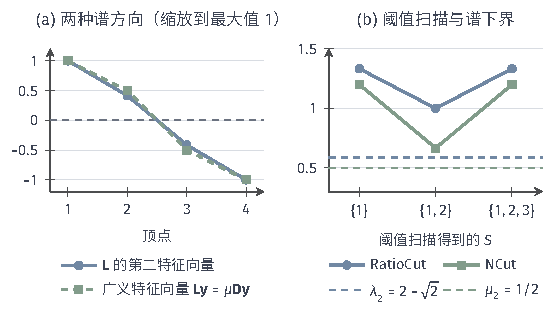
\includegraphics[width=94mm]{figures/01-basic-mathematics/04-graphs/tikz/c6-four-path-sweep/figure.pdf}
  \caption{单位权四点路径$1-2-3-4$上的两种谱划分。(a)~$\bm L$的第二特征向量（蓝）与广义特征问题$\bm L\bm y=\mu\bm D\bm y$的第二特征向量（绿），均按最大绝对值缩放到$1$；二者在零点两侧给出同样的分组，但中间两点的相对幅度不同。(b)~按坐标排序扫描三个阈值得到的原目标值，实线为RatioCut与NCut，虚线为相应谱下界$\lambda_2=2-\sqrt2$与$\mu_2=\tfrac12$；两种目标都在$S=\{1,2\}$处最小，且严格高于下界。}
  \label{fig:graph-spec-four-path-sweep}
\end{figure}

\paragraph{四点路径算例}
取单位权四点路径$1-2-3-4$。它的拉普拉斯的特征值为$0$、$2-\sqrt2$、$2$、$2+\sqrt2$，第二特征向量正比于$(1+\sqrt2,1,-1,-1-\sqrt2)^{\top}$；可以直接核对$\bm L\bm v=(2-\sqrt2)\bm v$。按坐标扫描得到三个候选分组，RatioCut依次为
\[
 S=\{1\}:\ 1\cdot\bigl(1+\tfrac13\bigr)=\tfrac43,\qquad
 S=\{1,2\}:\ 1\cdot\bigl(\tfrac12+\tfrac12\bigr)=1,\qquad
 S=\{1,2,3\}:\ \tfrac43 ,
\]
所以$U=1$。枚举全部七种非空二分，离散最优值也是$1$，在$\{1,2\}|\{3,4\}$处取到。谱下界为$\lambda_2=2-\sqrt2\approx0.586$，严格小于$1$，见图~\ref{fig:graph-spec-four-path-sweep}。这说明松弛通常不紧：这里恢复的分组恰好最优，但只凭$U-L\approx0.414$并不能确认这一点。

\paragraph{开销}
整个方法的开销分三部分。求$\bm u_2$：稠密完整特征分解需要$O(n^3)$时间、$O(n^2)$空间；大型稀疏图常用只求少数特征向量的迭代方法，其代价取决于求解器、所需精度和$\lambda_2$与$\lambda_3$的间隔，不能只因为$\bm L$稀疏就断言是线性时间。排序需要$O(n\log n)$。扫描时每个顶点移动一次，每条正权边被访问常数次，需要$O(n+m_+)$。

\subsection{NCut谱方法}
\label{sec:graph-spec-normalized-cut}

RatioCut用顶点个数衡量组的大小。另一种选择是用组内的连接总量：一组顶点的加权度之和
\[
 \operatorname{vol}(S)=\sum_{i\in S}d_i
\]
称为它的\term{体积}（volume）。设$p=\operatorname{vol}(S)>0$，$q=\operatorname{vol}(\bar S)>0$，定义\term{归一化割}（normalized cut，NCut）
\begin{equation}
 \operatorname{NCut}(S,\bar S)=\operatorname{cut}(S,\bar S)\Bigl(\frac1p+\frac1q\Bigr).
 \label{eq:graph-spec-normalized-cut}
\end{equation}
它要求两组的体积都为正。在图~\ref{fig:graph-spec-cut-indicator}中，顶点$7$的体积只有$0.6$，只切下它的NCut约为$1.04$；沿桥切开时两侧体积为$8.2$与$7$，NCut为$\tfrac1{8.2}+\tfrac17\approx0.26$，是全部非空二分中的最小值。

\paragraph{度加权的两水平向量}
与RatioCut平行，构造$y_i=\sqrt{q/p}$（$i\in S$）、$y_i=-\sqrt{p/q}$（$i\in\bar S$）。这次用度加权核对：
\[
 \bm y^{\top}\bm D\bm1=p\sqrt{q/p}-q\sqrt{p/q}=0,\qquad
 \bm y^{\top}\bm D\bm y=p\cdot\tfrac qp+q\cdot\tfrac pq=\operatorname{vol}(V),
\]
跨组边上的差为$\sqrt{q/p}+\sqrt{p/q}=(p+q)/\sqrt{pq}$，所以$\bm y^{\top}\bm L\bm y=\operatorname{cut}(S,\bar S)(p+q)^2/(pq)=\operatorname{vol}(V)\operatorname{NCut}(S,\bar S)$。于是
\[
 \operatorname{NCut}(S,\bar S)=\frac{\bm y^{\top}\bm L\bm y}{\bm y^{\top}\bm D\bm y},\qquad \bm y^{\top}\bm D\bm1=0 .
\]
与RatioCut相比，正交条件和长度都换成了度加权的版本，这正是第~\ref{sec:graph-spec-degree-inner-product}小节的度加权内积。两种方法采用了不同的平衡尺度。

\paragraph{化为对称归一化拉普拉斯}
先把谱计算限制在正度顶点$V_+$上。支撑孤点的体积为零，会让$\bm D$奇异，还会给$\bm L_{\mathrm{sym}}$带来额外的零特征向量$\bm e_v$，它们对应的并不是合法的正体积分组；孤点的处理放在下面单独说明。在$V_+$上$\bm D$正定，作坐标代换$\bm x=\bm D^{1/2}\bm y$，则
\[
 \frac{\bm y^{\top}\bm L\bm y}{\bm y^{\top}\bm D\bm y}=\frac{\bm x^{\top}\bm L_{\mathrm{sym}}\bm x}{\bm x^{\top}\bm x},\qquad
 \bm y^{\top}\bm D\bm1=\bm x^{\top}\bm D^{1/2}\bm1=0 .
\]
约束变成$\bm x\perp\bm D^{1/2}\bm1$，而$\bm D^{1/2}\bm1$正是$\bm L_{\mathrm{sym}}$的零特征向量（第~\ref{sec:graph-spec-null-space-components}小节）。取$\bm L_{\mathrm{sym}}$的标准正交特征基，使第一个向量为$\bm D^{1/2}\bm1/\lVert\bm D^{1/2}\bm1\rVert_2$，重复定理~\ref{thm:graph-spec-ratio-cut-bound}的证明，可知松弛问题的最小值是$\bm L_{\mathrm{sym}}$的第二小特征值$\mu_2$，在相应特征向量$\bm x_2$处取到，并且每个合法分组都有$\operatorname{NCut}\geq\mu_2$。

换回原坐标$\bm y_2=\bm D^{-1/2}\bm x_2$，由$\bm L_{\mathrm{sym}}\bm x_2=\mu_2\bm x_2$左乘$\bm D^{1/2}$得
\[
 \bm L\bm y_2=\mu_2\bm D\bm y_2 ,
\]
这是一个广义特征问题（定义~\ref{def:matrix-analysis-generalized-eigenvalue}），也可写成$\bm L_{\mathrm{rw}}\bm y_2=\mu_2\bm y_2$。阈值扫描应当使用$\bm y_2$的坐标。一般的非正则图上，不能用组合拉普拉斯的第二特征向量代替它：只有每个顶点度都等于同一个$d$时，$\bm L_{\mathrm{sym}}=\bm L/d$，两种方向才相同，特征值相差因子$d$。

\paragraph{分量、孤点与合法性}
若正度顶点组成多个正权支撑分量，每个分量的体积都为正，把其中一部分分量放进$S$、其余放进$\bar S$，割权为零，NCut为零，已经最优。此时$\mu_2=0$，零特征空间是多维的，其中任意一个向量都是“第二特征向量”，应直接按分量分组，分量可以由第~\ref{sec:graph-connectivity-computation}节的遍历求出。支撑孤点不影响割权，也不影响体积，求出正度部分的分组后可以把它们放进任一组。若$E_+$为空，所有顶点的体积都是零，当前NCut问题没有合法的二分；只要有一条正权边，把它的两个端点分到两侧就得到两个正体积组。所以恢复时要检查两组非空且体积为正，再重新计算原NCut。

\paragraph{四点路径上的对照}
回到单位权四点路径，$\bm D=\operatorname{diag}(1,2,2,1)$。广义特征问题的第二特征值为$\mu_2=\tfrac12$，特征向量正比于$\bm y_2=(1,\tfrac12,-\tfrac12,-1)^{\top}$；直接核对$\bm L\bm y_2=(\tfrac12,\tfrac12,-\tfrac12,-\tfrac12)^{\top}=\tfrac12\bm D\bm y_2$。扫描得到的NCut依次为$\tfrac65$、$\tfrac23$、$\tfrac65$，枚举全部七种二分可知离散最优值为$\tfrac23$，同样在$\{1,2\}|\{3,4\}$处取到，严格高于下界$\tfrac12$。与RatioCut比较，图~\ref{fig:graph-spec-four-path-sweep}显示两种谱方向在中间两点的相对幅度不同（$\tfrac1{1+\sqrt2}\approx0.41$对$\tfrac12$），目标函数和下界也不同，只是在这个小例子中恰好给出同一个分组。

最后提醒一点。若第二特征值是重特征值，对应特征空间中的任何单位向量都可能被数值程序返回，单个向量坐标的变化不代表图的结构发生了变化；这时应考察整个特征子空间，或者在其中比较多个候选方向的扫描结果。

% 第6章第8节：本章小结。

\section{本章小结}
\label{sec:graph-spectral-summary}

本章沿“顶点值—边差—加权汇总—谱坐标—滤波或划分”一路推进。关联矩阵的转置把顶点函数变成边差，按边权缩放后再汇总回顶点，就得到组合拉普拉斯$\bm L=\bm B\bm W_E\bm B^{\top}=\bm D-\bm W$，其二次型是沿边变化能量。连接总量不均时，度加权内积与坐标缩放给出$\bm L_{\mathrm{sym}}$，邻域平均给出$\bm L_{\mathrm{rw}}$，表~\ref{tab:graph-spec-laplacian-comparison}汇总了三者的差别。谱定理把这些算子的特征向量排成从平缓到剧烈的模态：零特征值的重数等于正权支撑分量数，$\bm L_{\mathrm{sym}}$的谱落在$[0,2]$中。在此基础上要分清三组区别：沿边变化能量按特征值加权，幅值平方不加权；图傅里叶变换只换坐标，滤波才改变函数；谱松弛给出下界和候选方向，离散分组必须经阈值扫描恢复，并用原目标重新计算。

\begin{table}[!htb]
  \centering\small
  \begin{tabularx}{\linewidth}{@{}lXXX@{}}
    \toprule
    & $\bm L$ & $\bm L_{\mathrm{sym}}$ & $\bm L_{\mathrm{rw}}$\\
    \midrule
    正度部分的定义 & $\bm D-\bm W$ & $\bm D^{-1/2}\bm L\bm D^{-1/2}$ & $\bm I-\bm D^{-1}\bm W$\\
    比较的量 & 相邻顶点的原值之差 & 除以$\sqrt{d_i}$后的值之差 & 本点值与邻居平均之差\\
    对称性 & 欧氏内积下对称 & 欧氏内积下对称 & 度加权内积下自伴\\
    每个分量的零模 & 指示向量$\bm1_C$ & $\bm D^{1/2}\bm1_C$；孤点为$\bm e_v$ & 指示向量$\bm1_C$\\
    谱的范围 & $[0,2d_{\max}]$，随边权尺度变化 & $[0,2]$ & 与$\bm L_{\mathrm{sym}}$相同\\
    支撑孤点 & 行列为零 & 约定$\bm D^{-1/2}$该处为$0$，行列为零 & 约定$(\bm P_{\mathrm{rw}})_{v,v}=1$，该行为零\\
    \bottomrule
  \end{tabularx}
  \caption{同一非负权图上三种拉普拉斯的对照。“分量”指正权支撑图的连通分量。$\bm L_{\mathrm{sym}}$与$\bm L_{\mathrm{rw}}$在正度顶点上相似，特征值相同，特征向量相差因子$\bm D^{1/2}$；三者的特征向量不能直接互换。}
  \label{tab:graph-spec-laplacian-comparison}
\end{table}

回看整个部分：第~\ref{chap:graph-objects}章建立了图、路径、连通与矩阵表示；第~\ref{chap:graph-traversal}章用遍历提取连通结构、拓扑次序和结构标记；第~\ref{chap:graph-optimization}章在路径、生成树、流和匹配上求最优；第~\ref{chap:graph-set-functions}章把评价对象扩展到子集；第~\ref{chap:graph-dynamic-programming}章利用局部依赖结构计算有限配置。前五章的对象都是离散的，本章转向挂在顶点上的数值，增加的是图算子与特征坐标这两样工具。它们并不取代前面的算法：判断连通仍可以直接遍历，最小割仍有精确的流算法，谱方法只在自己的条件下给出能量、坐标、滤波和松弛下界。随机游走的概率解释、连续扩散的演化和完整的傅里叶计算留到后续部分接续；本章所用的谱理论始终停留在有限维线性代数的范围内。


